\documentclass[11pt]{book}

\tolerance=600

% for \begin{center}, etc.
\usepackage[margin=1.0in]{geometry}

\usepackage{seqsplit}

% all kinds of math macros
\usepackage{amsmath}
\usepackage{amssymb}

% eps figures
\usepackage{epsfig}

% chapter title styles
\usepackage[Sonny]{fncychap}
\ChNameVar{\LARGE}
\ChTitleVar{\LARGE\sl}

% index
\usepackage{makeidx}
\makeindex


% part page style see
% http://tex.stackexchange.com/questions/6609/problems-with-part-labels-using-titlesec
\usepackage{titlesec}

\titleformat{\part}[display]
   {\Huge\filcenter}
   {{\partname{}} \thepart}
   {0em}
   {\hrule}



% hyperlinks -- load after fncychap
\usepackage{hyperref}

% color package
\usepackage[usenames]{color}

% longtable package used to split tables across pages
\usepackage{longtable}

% PDF-aware landscape package, used for rotating tables (including the
% longtable)
\usepackage{pdflscape}

% table coloring
\usepackage{colortbl}
\definecolor{tableShade}{rgb}{0.945,0.961,0.980}


% make the MarginPars look pretty
\setlength{\marginparwidth}{0.75in}
\newcommand{\MarginPar}[1]{\marginpar{\vskip-\baselineskip\raggedright\tiny\sffamily
\hrule\smallskip{\color{red}#1}\par\smallskip\hrule}}

% to increase the likelihood that floats will occur "here" when you
% want them to
\renewcommand{\floatpagefraction}{1.0}
\renewcommand{\topfraction}{1.0}
\renewcommand{\bottomfraction}{1.0}
\renewcommand{\textfraction}{0.0}

% number subsubsections and put them in the TOC
\setcounter{tocdepth}{3}
\setcounter{secnumdepth}{3}

% custom hrule for title page
\newcommand{\HRule}{\rule{\linewidth}{0.125mm}}

% control sequences in verbatim
\usepackage{fancyvrb}

% short table of contents
\usepackage{shorttoc}

% spacing in the table of contents
\usepackage[titles]{tocloft}

\setlength{\cftbeforechapskip}{2ex}
\setlength{\cftbeforesecskip}{0.25ex}

% For splitting up lists into multitple columns
\usepackage{multicol}

% don't put a header on blank pages, see
% http://www.latex-community.org/forum/viewtopic.php?f=4&p=51559
% change ``plain'' to ``empty'' to eliminate the page number
\makeatletter
\renewcommand*\cleardoublepage{\clearpage\if@twoside
\ifodd\c@page\else
\hbox{}
\thispagestyle{empty}
\newpage
\if@twocolumn\hbox{}\newpage\fi\fi\fi}
\makeatother


% don't make the chapter/section headings uppercase.  See the fancyhdr
% documentation (section 9)
\usepackage{fancyhdr}
\renewcommand{\chaptermark}[1]{%
 \markboth{\chaptername
\ \thechapter.\ #1}{}}

\renewcommand{\sectionmark}[1]{\markright{\thesection---#1}}

\graphicspath{{Verification/}{Software/}{ConvertCheckpoint/}{Scaling/}{Visualization/}{Particles/}{Rotation/}}

% skip a bit of space between paragraphs, to enhance readability
\usepackage{parskip}



% special fraction
\newcommand{\sfrac}[2]{\mathchoice
  {\kern0em\raise.5ex\hbox{\the\scriptfont0 #1}\kern-.15em/
   \kern-.15em\lower.25ex\hbox{\the\scriptfont0 #2}}
  {\kern0em\raise.5ex\hbox{\the\scriptfont0 #1}\kern-.15em/
   \kern-.15em\lower.25ex\hbox{\the\scriptfont0 #2}}
  {\kern0em\raise.5ex\hbox{\the\scriptscriptfont0 #1}\kern-.2em/
   \kern-.15em\lower.25ex\hbox{\the\scriptscriptfont0 #2}}
  {#1\!/#2}}

\def\Ab {{\bf A}}
\def\eb {{\bf e}}
\def\Fb {{\bf F}}
\def\gb {{\bf g}}
\def\Hb {{\bf H}}
\def\ib {{\bf i}}
\def\Ib {{\bf I}}
\def\Kb {{\bf K}}
\def\lb {{\bf l}}
\def\Lb {{\bf L}}
\def\nb {{\bf n}}
\def\Pb {{\bf P}}
\def\Qb {{\bf Q}}
\def\rb {{\bf r}}
\def\Rb {{\bf R}}
\def\Sb {{\bf S}}
\def\ub {{\bf u}}
\def\Ub {{\bf U}}
\def\xb {{\bf x}}

\def\dt       {\Delta t}
\def\omegadot {\dot\omega}

\def\inp  {{\rm in}}
\def\outp {{\rm out}}
\def\sync {{\rm sync}}

\def\half   {\frac{1}{2}}
\def\myhalf {\sfrac{1}{2}}
\def\nph    {{n+\myhalf}}


% Radiation
%\newcommand{\kpp}{\ensuremath{\kappa_{\mathrm{P}}}}
%\newcommand{\kpr}{\ensuremath{\kappa_{\mathrm{R}}}}
%\newcommand{\kpf}{\ensuremath{\kappa_{\mathrm{F}}}}

% Rotation
\newcommand{\vb}{\boldsymbol{v}}
\newcommand{\vbt}{\widetilde{\vb}}
\newcommand{\rbt}{\widetilde{\rb}}
\newcommand{\ob}{\boldsymbol{\omega}}
\newcommand{\nablab}{\boldsymbol{\nabla}}

% codes
\newcommand{\castro}{{\sf Castro}}
\newcommand{\maestro}{{\sf Maestro}}
\newcommand{\boxlib}{{\sf BoxLib}}
\newcommand{\microphysics}{{\sf Microphysics}}
\newcommand{\yt}{{\sf yt}}
\newcommand{\amrvis}{{\sf Amrvis}}
\newcommand{\visit}{{\sf VisIt}}

\newcommand{\cpp}{C\nolinebreak\hspace{-.05em}\raisebox{.4ex}{\tiny\bf +}\nolinebreak\hspace{-.10em}\raisebox{.4ex}{\tiny\bf +}}

\newcommand{\multifab}{{\tt MultiFab}}
\newcommand{\statedata}{{\tt StateData}}


\usepackage{listings}

\definecolor{gray}{rgb}       {0.8,0.8,0.8}
\definecolor{light-blue}{rgb} {0.8,0.8,1.0}
\definecolor{light-green}{rgb}{0.8,1.0,0.8}
\definecolor{light-red}{rgb}  {1.0,0.9,0.9}

\lstset{
  basicstyle=\small\ttfamily,%
  frame=single,%
  rulesepcolor=\color{gray},%
  backgroundcolor=\color{white}%
}
\lstset{belowskip=-0.25em}


% Macros for indexing
\newcommand\nott[1]{\bgroup\let\tt\relax#1\egroup}

\newcommand{\runparam}[1]{\index{Runtime parameters!{\tt #1}}{\tt #1}}

% this variant doesn't write the name of the namespace in the latex
% but does use it in the index
\newcommand{\runparamNS}[2]{\index{Runtime parameters!{\tt #2.#1}}{\tt #1}}
\newcommand{\runparamidx}[1]{\index{Runtime parameters!{\tt #1}}}

\newcommand{\code}[1]{\index{Code reference!#1@{\tt #1}}{\tt #1}}
\newcommand{\codeidx}[1]{\index{Code reference!#1@{\tt #1}}}

\newcommand{\ifdef}[1]{\index{Preprocessor!{\tt #1}}{\textcolor{blue}{\tt #1}}}
\newcommand{\problem}[1]{\index{Problem setups!{\tt #1}}{\tt #1}}
\newcommand{\makevar}[1]{\index{Makefiles!{\tt #1}}{\tt #1}}
\newcommand{\variable}[1]{\index{Variables!{\tt #1}}{\tt #1}}

\newcommand{\otherindex}[2]{\index{#1!#2}}



%------------------------------------------------------------------------------
\begin{document}

\frontmatter

\begin{titlepage}
\begin{center}
\ \\[3in]
{\sf \Huge CASTRO}

\begin{minipage}{5.5in}
\HRule\\[2mm]
\centering
{\Large \em An adaptive, parallel, radiation hydrodynamics code\\ for self-gravitating astrophysical flows}

\HRule
\end{minipage}

\ \\[1 in]
{\sf \huge User's Guide}

\vfill

{\large \today}
\end{center}

\end{titlepage}


\shorttoc{Chapter Listing}{0}

\setcounter{tocdepth}{2}
\tableofcontents

\clearpage

\listoffigures
\addcontentsline{toc}{chapter}{list of figures}

\clearpage

\listoftables
\addcontentsline{toc}{chapter}{list of tables}

\clearpage

\chapter*{Preface}
\chaptermark{Preface}
\addcontentsline{toc}{chapter}{preface}


Welcome to the \castro\ User's Guide!

In this User's Guide we describe how to download and run \castro, a
massively parallel code that solves the multicomponent compressible
hydrodynamic equations for astrophysical flows including self-gravity,
nuclear reactions and radiation.  \castro\ uses an Eulerian grid and
incorporates adaptive mesh refinement (AMR).  Our approach to AMR uses
a nested hierarchy of logically-rectangular grids with simultaneous
refinement in both space and time, utilizing the
\amrex\ library\footnote{earlier versions of \castro\ used the
  \boxlib\ library}.

The core algorithms in \castro\ are described in a series of papers:
\begin{itemize}
\item {\it CASTRO: A New Compressible Astrophysical Solver. I. Hydrodynamics and Self-gravity},
  A.~S.~Almgren, V.~E.~Beckner, J.~B.~Bell, M.~S.~Day, L.~H.~Howell, C.~C.~Joggerst, M.~J.~Lijewski,
  A.~Nonaka, M.~Singer, \& M.~Zingale, 2010, ApJ, 715, 1221\newline
  \url{http://dx.doi.org/10.1088/0004-637X/715/2/1221}

\item {\it CASTRO: A New Compressible Astrophysical Solver. II. Gray Radiation Hydrodynamics},
  W.~Zhang, L.~Howell, A.~Almgren, A.~Burrows, \& J.~Bell, 2011, ApJS, 196, 20\newline
  \url{http://dx.doi.org/10.1088/0067-0049/196/2/20}

\item {\it CASTRO: A New Compressible Astrophysical Solver. III. Multigroup Radiation Hydrodynamics},
  W.~Zhang, L.~Howell, A.~Almgren, A.~Burrows, J.~Dolence, \& J.~Bell, 2013, ApJS, 204, 7\newline
  \url{http://dx.doi.org/10.1088/0067-0049/204/1/7}

\end{itemize}

Improvements to the gravity solver and rotation were described in:
\begin{itemize}
\item {\it Double White Dwarf Mergers on Adaptive Meshes I. Methodology
       and Code Verification, }
  M.~P.~Katz, M.~Zingale, A.~C.~Calder, F.~D.~Swesty, A.~S.~Almgren, W.~Zhang
  2016, ApJ, 819, 94.\newline
  \url{http://dx.doi.org/10.3847/0004-637X/819/2/94}
\end{itemize}

The development of \amrex\ library is led by the
Center for Computational Sciences and Engineering / Lawrence Berkeley
National Laboratory.  \castro\ development is done collaboratively,
including the CCSE and Stony Brook University.

\castro\ {\em core developers} are those who have made substantial
contributions to the code.  The process for becoming a core developer
is described in the {\tt README.md} in the \castro\ root directory.
Current \castro\ core developers are:

% git shortlog -sn
\begin{quote}
Ann Almgren\newline
Maria G.\ Barrios Sazo\newline
John Bell\newline
Vince Beckner\newline
Marc Day\newline
Max Katz\newline
Mike Lijewski\newline
Chris Malone\newline
Andy Nonaka\newline
Weiqun Zhang\newline
Michael Zingale
\end{quote}

All \castro\ development takes place on the project's github
page\\[0.5em] \url{https://github.com/AMReX-Astro/Castro}\\[0.5em]
External contributions are welcomed.  Fork the \castro\ repo, modify
your local copy, and issue a pull-request to the {\tt
  AMReX-Astro/Castro} project.  Further guidelines are given in the
{\tt README.md} file.

To get help, subscribe to the {\em castro-help} google group mailing list:
\url{https://groups.google.com/forum/#!forum/castro-help}


\section*{Acknowledging and Citing \castro}

If you use \castro\ in your research, we would appreciate it if you
cited the relevant code papers describing its design, features, and
testing.  A list of these can be found in the
\href{https://github.com/AMReX-Astro/Castro/blob/master/CITATION}{\tt
  CITATION} file in the root {\tt Castro/} directory.

The development \castro\ is supported by the science application
interests of the contributors.  There is a lot of effort behind the
scenes: testing, optimization, development of new features, bug
fixing, $\ldots$, that is often done under the radar.  Nevertheless,
we are happy to volunteer our time to help new users come up to speed
with \castro.  When significant new development / debugging for you
application is provided by a member of the \castro\ development
community, we would appreciate consideration of inviting the
developer(s) for co-authorship on any science paper that results.


\clearpage

\mainmatter

\chapter{Introduction}
\section{Introduction to \castro}

\castro\ is a adaptive mesh, radiation hydrodynamics code that is
designed to model astrophysical reacting flows on massively parallel
computers.

The major capabilities:
\begin{itemize}
\item 1-, 2-, and 3-dimensional unsplit, 2nd-order hydrodynamics
\item multigroup flux-limited diffusion radiation hydrodynamics
\item adaptive mesh refinement with subcycling; jumps of 2x and 4x between levels
\item arbitrary equation of state (gamma-law and stellar EOSes are bundled)
\item general nuclear reaction networks
\item explicit thermal diffusion
\item full Poisson gravity (with isolated boundary conditions)
\item rotation (in the co-rotating frame) in 2-d axisymmetric and 3-d.
\item parallelization via MPI + OpenMP
\end{itemize}



\section{Units and Conventions}

\castro\ works in CGS units unless otherwise specified.
Table~\ref{table:units} shows some of the common symbols / names used
throughout the code documentation and papers.

\begin{table}[t]
\renewcommand{\arraystretch}{1.2}
\centering
\begin{tabular}{lll}
name & units & description \\
\hline
$t$    & s       & time \\
$\rho$ & $\gcc$  & mass density \\
$\ub$  & $\cms$  & velocity vector \\
$p$    & $\presunit$ & pressure \\
$\gb$  & $\accelunit$ & gravitational acceleration \\
$\Sb$  & varies       & source term \\
$E$    & $\ergg$      & specific total energy \\
$e$    & $\ergg$      & specific internal energy \\
$T$    & $K$          & temperature \\
$\kth$ & $\mathrm{erg~cm^{-1}~s^{-1}~K~{-1}}$ & thermal conductivity \\
$X_k$  & --           & mass fraction of species $k$ \\
$\omegadot_k$ & $\mathrm{s^{-1}}$  & species creation rate (from reactions) \\
\hline
\end{tabular}
\caption{\label{table:units} Common quantities and units.}
\renewcommand{\arraystretch}{1.0}
\end{table}

Physical constants, again using the CGS system are available 
in {\tt Castro/constants/constants\_cgs.f90}



\chapter{Getting Started}

\section{Downloading the Code}

\castro\ is built on top of the \amrex\ framework.  In order to run
\castro\, you must download two separate git modules.

\vspace{.1in}

\noindent First, make sure that {\tt git} is installed on your machine---we recommend version 1.7.x or higher.

\vspace{.1in}

\begin{enumerate}

\item Clone/fork the \amrex\ repository from the {\tt AMReX-Codes} {\sf
  github} page (\url{https://github.com/AMReX-Codes/amrex/}).  To
  clone via the command line, simply type:
\begin{verbatim}
git clone https://github.com/AMReX-Codes/amrex.git
\end{verbatim}
Alternately, if you have a {\sf github} account with your
machine's SSH-keys registered, you can do:
\begin{verbatim}
git clone ssh://git@github.com/AMReX-Codes/amrex.git
\end{verbatim}

This will create a directory called {\tt amrex/} on your machine.

You will want to periodically update \amrex\ by typing
\begin{verbatim}
git pull
\end{verbatim}
in the {\tt amrex/} directory.  

Note: actively development is done on the {\tt development} branch
in each repo, and merged into the {\tt master} branch periodically.
If you wish to use the \castro\ {\tt development} branch, then you
should also switch to the {\tt development} branch for \amrex.

\item Set the environment variable, {\tt AMREX\_HOME}, on your
  machine to point to the path name where you have put \amrex.
  You can add this to your {\tt .bashrc} as:
\begin{Verbatim}[commandchars=\\\{\}]
export AMREX_HOME={\em /path/to/amrex/}
\end{Verbatim}
where you replace \texttt{\em /path/to/amrex/} will the full path to the
{\tt amrex/} directory.

\item Clone/fork the \castro\ repository from the same {\sf
  github} organization as above, using either HTTP access:
\begin{verbatim}
git clone https://github.com/AMReX-Astro/Castro.git
\end{verbatim}
or SSH access if you have it enabled:
\begin{verbatim}
git clone ssh://git@github.com:/AMReX-Astro/Castro.git
\end{verbatim}
Or, as above, you can download a ZIP file of the code from
\href{https://github.com/AMReX-Astro}{our main {\sf github} page},
by clicking on the \castro\ link.

As with \amrex, development on \castro\ is done in the
{\tt development} branch, so you should work there if you want
the latest source.

\item We recommend setting the {\tt CASTRO\_HOME} environment
  variable to point to the path name where you have put \castro.
  Add the following to your {\tt .bashrc}:
\begin{verbatim}
export CASTRO_HOME="/path/to/Castro/"
\end{verbatim}


\item (optional) An additional repository, {\tt Microphysics.git} is
  available at the {\tt starkiller-astro} github page.  This add
  additional reaction networks and EOSes and can be cloned following
  the same procedure as above\footnote{Note: previously the radiation
    solver was distributed separately as {\tt CastroRadiation.git},
    but this has been merged into the main \castro\ respository}:
\begin{verbatim}
git clone https//github.com/starkiler-astro/Microphysics.git
\end{verbatim}
or via SSH as
\begin{verbatim}
git clone ssh://git@github.com:/starkiler-astro/Microphysics.git
\end{verbatim}

To access the \microphysics\ routines, set the {\tt MICROPHYSICS\_HOME}
environment variable to point to the {\tt Microphysics/} directory.

\end{enumerate}

%\clearpage

\section{Building the Code}

In \castro\ each different problem setup is stored in its own
sub-directory under {\tt Castro/Exec/}.  You build the
\castro\ executable in the problem sub-directory.  Here we'll
build the {\tt Sedov} problem:

\begin{enumerate}

\item From the directory in which you checked out the Castro git repo,
  type
\begin{verbatim}
cd Castro/Exec/hydro_tests/Sedov
\end{verbatim}
This will put you into a directory in which you can run the Sedov
problem in 1-d, 2-d or 3-d.

\item In {\tt Sedov/}, edit the {\tt GNUmakefile}, and set
  \begin{itemize}
    \item \makevar{DIM} {\tt = 2} 

      This is the dimensionality---here we pick 2-d.

    \item \makevar{COMP} {\tt = gnu}

      This is the set of compilers.  {\tt gnu} are a good default
      choice (this will use {\tt g++} and {\tt gfortran}.  You can
      also choose {\tt pgi} and {\tt intel} for example.

      If you want to try other compilers than the GNU suite and they
      don't work, please let us know.

    \item \makevar{DEBUG} {\tt = FALSE}

      This disabled debugging checks and results in a more
      optimized executable.

    \item \makevar{USE\_MPI} {\tt = FALSE}

      This turns off parallelization via MPI.  Set it to {\tt TRUE} to
      build with MPI---this requires that you have the MPI library
      installed on your machine.  In this case, the build system will
      need to know about your MPI installation.  This can be done by
      editing the makefiles in the \amrex\ tree, but the default
      fallback is to look for the standard MPI wrappers (e.g.\ {\tt
        mpic++} and {\tt mpif90}) to do the build.

  \end{itemize}

\item Now type {\tt make}.

  The resulting executable will look something like {\tt
    Castro2d.Linux.gnu.ex}, which means this is a 2-d version
  of the code, made on a Linux machine, with {\tt COMP = gnu}.

\end{enumerate}

\section{Running the Code}

\begin{enumerate}

\item \castro\ takes an input file that overrides the runtime parameter defaults.
  The code is run as:
\begin{verbatim}
Castro2d.Linux.gcc.gfortran.ex inputs.2d.cyl_in_cartcoords
\end{verbatim}

This will run the 2-d cylindrical Sedov problem in Cartesian ($x$-$y$
coordinates).  You can see other possible options, which should be
clear by the names of the inputs files.

\item You will notice that running the code generates directories that
  look like {\tt plt00000/}, {\tt plt00020/}, etc, and {\tt chk00000/},
  {\tt chk00020/}, etc. These are ``plotfiles'' and ``checkpoint''
  files. The plotfiles are used for visualization, the checkpoint
  files are used for restarting the code.

\end{enumerate}

\section{Visualization of the Results}
\index{visualization}

There are several options for visualizing the data.  The popular
\visit\ package supports the \amrex\ file format natively, as does the
\yt\ python package\footnote{Each of these will recognize it as the
  \boxlib\ format.}.  The standard tool used within the
\boxlib-community is \amrvis, which we demonstrate here.

\begin{enumerate}

\item Get \amrvis:

\begin{verbatim}
git clone https://ccse.lbl.gov/pub/Downloads/Amrvis.git
\end{verbatim}

Then cd into {\tt Amrvis/}, edit the {\tt GNUmakefile} there
to set {\tt DIM = 2}, and again set {\tt COMP} to compilers that
you have. Leave {\tt DEBUG = FALSE}.

Type {\tt make} to build, resulting in an executable that
looks like {\tt amrvis2d...ex}.

If you want to build amrvis with {\tt DIM = 3}, you must first
download and build {\tt volpack}:
\begin{verbatim}
git clone https://ccse.lbl.gov/pub/Downloads/volpack.git
\end{verbatim}

Then cd into {\tt volpack/} and type {\tt make}.

Note: \amrvis\ requires the OSF/Motif libraries and headers. If you don't have these 
you will need to install the development version of motif through your package manager. 
On most Linux distributions, the motif library is provided by the
{\tt openmotif} package, and its header files (like {\tt Xm.h}) are provided
by {\tt openmotif-devel}.  If those packages are not installed, then use the
package management tool to install them, which varies from
distribution to distribution, but is straightforward. 
{\tt lesstif} gives some functionality and will allow you to build the amrvis executable, 
but \amrvis\ may not run properly.

You may then want to create an alias to {\tt amrvis2d}, for example
\begin{verbatim}
alias amrvis2d /tmp/Amrvis/amrvis2d...ex
\end{verbatim}
where {\tt /tmp/Amrvis/amrvis2d...ex} is the full path and name of the \amrvis\ executable.

\item Configure \amrvis:  

  Copy the {\tt amrvis.defaults} file to your home directory (you can
  rename it to {\tt .amrvis.defaults} if you wish).  Then edit the
  file, and change the {\tt palette} line to point to the full
  path/filename of the {\tt Palette} file that comes with \amrvis.

\item Visualize:

  Return to the {\tt Castro/Exec/hydro\_tests/Sedov} directory.  You should
  have a number of output files, including some in the form {\tt *pltXXXXX},
  where {\tt XXXXX} is a number corresponding to the timestep the file
  was output.  {\tt
    amrvis2d {\em filename}} to see a single plotfile, or {\tt amrvis2d -a
  *plt*}, which will animate the sequence of plotfiles.

  Try playing
  around with this---you can change which variable you are
  looking at, select a region and click ``Dataset'' (under View)
  in order to look at the actual numbers, etc. You can also export the
  pictures in several different formats under "File/Export".

Some users have found that \amrvis\ does not work properly under X
with the proprietary Nvidia graphics driver.  A fix for this is
provided in the FAQ (\S~\ref{ch:faq:vis})---this is due to the default
behavior of the DAC in mappuing colors.  

Note: \yt\ is a great alternative to using \amrvis\ for visualization,
and understands \castro\ plotfiles well.

Please know that we do have a number of conversion routines to other
formats (such as matlab), but it is hard to describe them all. If you
would like to display the data in another format, please let us know
(again, {\tt asalmgren@lbl.gov}) and we will point you to whatever we have
that can help.

\end{enumerate}

You have now completed a brief introduction to \castro. 


\section{Other Distributed Problem Setups}

There are a number of standard problem setups that come with \castro.
These can be used as a starting point toward writing your own setup.
We organize these into subdirectories by broad type (radiation, hydro,
gravity, etc.): The standard categories and {\em some} of the included
problems are:
\begin{itemize}
\item {\tt gravity\_tests}:

  \begin{itemize}
  \item {\tt DustCollapse}:

    A pressureless cloud collapse that is a standard test problem for
    gravity.  An analytic solution that describes the radius of the
    sphere as a function of time is found in Colgate and
    White~\cite{colgwhite}.  This problem is also found in the FLASH
    User's Guide.
    
  \item {\tt hydrostatic\_adjust}:

    Model a 1-d stellar atmosphere (plane-parallel or
    spherical/self-gravitating) and dump energy in via an analytic
    heat source and watch the atmosphere's hydrostatic state adjust in
    response.  This is the counterpart to the \maestro\ {\tt
      test\_basestate} unit test.

  \end{itemize}


\item {\tt hydro\_tests}:

  \begin{itemize}
  \item {\tt double\_bubble}:

    Initialize 1 or 2 bubbles in a stratified atmosphere (isothermal
    or isentropic) and allow for the bubbles to have the same or a
    different $\gamma$ from one another / the background atmosphere.
    This uses the {\tt multigamma} EOS.

    An analogous problem is implemented in \maestro.
    
  \item {\tt HCBubble}:
  
  \item {\tt KH}:

    A Kelvin-Helmholtz shear instability problem.
  
  \item {\tt oddeven}:

    A grid-aligned shock hitting a very small density perturbation.
    This demonstrates the odd-even decoupling problem discussed in
    \cite{quirk1997}.  This setup serves to test the {\tt
      castro.hybrid\_riemann} option to hydrodynamics.
  
  \item {\tt reacting\_bubble}:

    A reacting bubble in a stratified white dwarf atmosphere.  This
    problem was featured in the \maestro\ reaction
    paper~\cite{maestro:III}.

  \item {\tt RT}:

    A single-model Rayleigh-Taylor instability problem.
  
  \item {\tt RT\_particles}:

  \item {\tt Sedov}:

    The standard Sedov-Taylor blast wave problem.  This setup was used
    in the first \castro\ paper~\cite{castro_I}.
    
  \item {\tt Sod}:
  
    A one-dimensional shock tube setup, including the classic Sod
    problem.  This setup was used in the original \castro\ paper.
  
  \item {\tt Sod\_stellar}:

    A version of the Sod shock tube for the general stellar equation
    of state.  This setup and the included inputs files was used
    in~\cite{zingalekatz}.

  \item {\tt toy\_convect}:

    A simple nova-like convection problem with an external heating
    source.  This problem shows how to use the model parser to
    initialize a 1-d atmosphere on the Castro grid, incorporate a
    custom tagging routine, sponge the fluid above the atmosphere, and
    write a custom diagnostics routine.

    A \maestro\ version of this problem setup also exists.
  \end{itemize}
    

\item{\tt radiation\_tests}:

\item{\tt science}:

\item{\tt unit\_tests}:


  
  
  
\end{itemize}


\chapter{Inputs Files}
The \castro\ executable uses two inputs files at runtime to set and alter the
behavior of the algorithm and initial conditions.

The main inputs file, typically named {\tt inputs}\index{{\tt inputs}}
is used to set \boxlib\ parameters and the control flow in the
\cpp\ portions of the \castro\ code.  Each parameter here has a
namespace (like {\tt amr.{\em optionname}} or {\tt castro.{\em
    optionname}}).  Parameters set here are read using the
\boxlib\ {\tt ParmParse} class infrastructure.

The second inputs file, typically named {\tt probin}\index{{\tt
    probin}} is used by the Fortran code that initializes the problem
setup.  It is read at problem initialization (via a Fortran {\tt
  namelist}) and the problem-specific quantities are stored in a
Fortran module \code{probdata\_module} defined in the problem's {\tt
  probdata.f90} file.

Only the {\tt inputs} file is specified on the commandline.  The
associated {\tt probin} file is specified in the {\tt inputs} file
using the {\tt amr.probin\_file} parameter, e.g.,
\begin{lstlisting}
amr.probin_file = my_special_probin
\end{lstlisting}
for example, has the Fortran code read a file called {\tt my\_special\_probin}.

\section{Working with {\tt probin} Files}

There are three different Fortran {\tt namelist}s that can be defined in the
{\tt probin} file:
\begin{itemize}
\item {\tt \&fortin} is the main {\tt namelist} read by the problem's {\tt probinit}
subroutine in the {\tt Prob\_?d.f90} file.

\item {\tt \&extern} is used to set different microphysics options

\item {\tt \&tagging} is used to get the parameters (defined in \code{tagging\_module})
that affect how we tag for refinement.
\end{itemize}

\section{Common {\tt inputs} Options}

{\bf Important}: because the {\tt inputs} file is handled by the \cpp\ portion of
the code, any quantities you specify in scientific notation, must take the
form {\tt 1.e5} and not {\tt 1.d5}---the `{\tt d}' specifier is not recognized.

Additionally, note that in \castro, all quantities are in CGS units.

\subsection{Problem Geometry}

The {\tt geometry} namespace is used by \boxlib\ to define the
computational domain.  The main parameters here are:
\begin{itemize}
\item \runparam{geometry.prob\_lo}: physical location of low corner of the
domain (type: {\tt Real}; must be set)

  Note: a number is needed for each dimension in the problem
  
\item \runparam{geometry.prob\_hi}: physical location of high corner of the
domain (type: {\tt Real}; must be set)

  Note: a number is needed for each dimension in the problem
  
\item \runparam{geometry.coord\_sys}: coordinate system, 0 = Cartesian,
1 = $r$-$z$ (2-d only), 2 = spherical (1-d only) (must be set)

\item \runparam{geometry.is\_periodic}: is the domain periodic in this direction?
  {\tt 0} if false, {\tt 1} if true  (default: {\tt 0 0 0}) 

  Note: an integer is needed for each dimension in the problem

\item {\tt castro.center}: physical location of problem center on the
  domain (type: {\tt Real}; default: {\tt 0.0 0.0 0.0}).  The problem
  center is used for gravity, rotation, and some other quantities.
  This is not necessarily the geometric center of the domain---often
  you should choose it to coincide with the center of mass of your
  system.  See \S~\ref{soft:prob_params} for more details.

  Note: a number is needed for each dimension in the problem

\end{itemize}

As an example, the following:
\begin{lstlisting}
geometry.prob_lo = 0 0 0
geometry.prob_hi = 1.e8 2.e8 2.e8 
geometry.coord_sys = 0 
geometry.is_periodic = 0 1 0 
castro.center = 5.e7 1.e8 1.e8
\end{lstlisting}

This defines the domain to run from $(0,0,0)$ at the lower left to
$(10^8,\, 2\times 10^8,\, 2\times 10^8)$ at the upper right in physical
space, specifies a Cartesian geometry, and makes the domain periodic
in the $y$-direction only. The problem center is set to be halfway in
between the lower left and upper right corners.


\subsection{Domain Boundary Conditions}

Boundary conditions are specified using integer keys that are interpreted
by \boxlib.  The runtime parameters that we use are:
\begin{itemize}
\item {\tt castro.lo\_bc}: boundary type of each low face  (must be set)
\item {\tt castro.hi\_bc}: boundary type of each high face (must be set)
\end{itemize}

The valid boundary types are:
\begin{table*}[h]
\begin{center}
\begin{tabular}{llll} 
{\tt 0} --  Interior / Periodic \hspace{1.in} & {\tt 3}  --  Symmetry     \hspace{1.in} & \\
{\tt 1} --  Inflow              \hspace{1.in} & {\tt 4}  --  Slip Wall    \hspace{1.in}& \\
{\tt 2} --  Outflow             \hspace{1.in} & {\tt 5}  --  No Slip Wall \hspace{1.in}& \\
\end{tabular}
\end{center}
\end{table*}

\noindent Note: {\tt castro.lo\_bc} and {\tt castro.hi\_bc} must be
consistent with {\tt geometry.is\_periodic}---if the domain is
periodic in a particular direction then the low and high bc's must be
set to {\tt 0} for that direction.

As an example, the following:
\begin{lstlisting}
castro.lo_bc = 1 4 0 
castro.hi_bc = 2 4 0 

geometry.is_periodic = 0 0 1
\end{lstlisting}

This defines a problem with inflow ({\tt 1}) in the low-$x$ direction,
outflow ({\tt 2}) in the high-$x$ direction, slip wall ({\tt 4}) on
the low and high $y$-faces, and periodic in the $z$-direction.
See \S~\ref{soft:phys_bcs} for more information.

\subsection{Resolution}

The grid resolution is specified by defining the resolution at the
coarsest level (level 0) and the number of refinement levels and
factor of refinement between levels.  The relevant parameters are:
\begin{itemize}
\item \runparam{amr.n\_cell}: number of cells in each direction at the
  coarsest level (Integer $> 0$; must be set)

\item \runparam{amr.max\_level}: number of levels of refinement above the
  coarsest level (Integer $\geq 0$; must be set)

\item \runparam{amr.ref\_ratio}: ratio of coarse to fine grid spacing
  between subsequent levels (2 or 4; must be set)

\item \runparam{amr.regrid\_int}: how often (in terms of number of steps)
  to regrid (Integer; must be set)

\item \runparam{amr.regrid\_on\_restart}: should we regrid immediately
  after restarting? (0 or 1; default: 0)
\end{itemize}

Note: if {\tt amr.max\_level = 0} then you do not need to set {\tt
  amr.ref\_ratio} or {\tt amr.regrid\_int}.

Some examples:
\begin{lstlisting}
amr.n_cell = 32 64 64
\end{lstlisting}
would define the domain to have 32 cells in the $x$-direction, 64 cells
in the $y$-direction, and 64 cells in the $z$-direction {\em{at the
coarsest level}}.  (If this line appears in a 2D inputs file then the
final number will be ignored.)\newline

\begin{lstlisting}
amr.max_level = 2 
\end{lstlisting}
would allow a maximum of 2 refined levels in addition to the coarse
level.  Note that these additional levels will only be created only if
the tagging criteria are such that cells are flagged as needing
refinement.  The number of refined levels in a calculation must be
$\leq$ {\tt amr.max\_level}, but can change in time and need not
always be equal to {\tt amr.max\_level}.  \newline
 
\begin{lstlisting}
amr.ref_ratio = 2 4 
\end{lstlisting}
would set factor of 2 refinement between levels 0 and 1, and factor of 4
refinement between levels 1 and 2.  Note that you must have at least
{\tt amr.max\_level} values of {\tt amr.ref\_ratio} (Additional values
may appear in that line and they will be ignored). \newline

\begin{lstlisting}
amr.regrid_int = 2 2
\end{lstlisting}
tells the code to regrid every 2 steps.  Thus in this example, new
level 1 grids will be created every 2 level-0 time steps, and new
level 2 grids will be created every 2 level-1 time steps. If {\tt
amr.regrid\_int} $<$ 0 for any level, then regridding starting at that
level will be disabled. If {\tt amr.regrid\_int = -1} only, then we
never regrid for any level. Note that this is not compatible with {\tt
amr.regrid\_on\_restart = 1}.


\subsection{Regridding}

The details of the regridding strategy are described in
\S~\ref{sec:tagging}; here we cover how the input parameters can
control the gridding.

As described later, the user defines Fortran subroutines which tag
individual cells at a given level if they need refinement.  This list
of tagged cells is sent to a grid generation routine, which uses the
Berger-Rigoutsos algorithm~\cite{br-refine} to create rectangular
grids that contain the tagged cells.

The relevant runtime parameters are:
\begin{itemize}
\item \runparam{amr.regrid\_file}: name of file from which to read the
  grids (text; default: no file)

  If set to a filename, e.g.\ {\tt fixed\_girds}, then list of grids
  at each fine level are read in from this file during the gridding
  procedure. These grids must not violate the {\tt
  amr.max\_grid\_size} criterion.  The rest of the gridding procedure
  described below will not occur if {\tt amr.regrid\_file} is set.

\item \runparam{amr.n\_error\_buf}: radius of additional tagging
  around already tagged cells (Integer $\geq 0$; default: 1)

\item \runparam{amr.max\_grid\_size}: maximum size of a grid in any
  direction (Integer $> 0$; default: 128 (2-d), 32 (3-d))

   Note: {\tt amr.max\_grid\_size} must be even, and a multiple of
   {\tt amr.blocking\_factor} at every level.
   
\item \runparam{amr.blocking\_factor}: grid size must be a multiple of this
  (Integer $> 0$; default: 2)

   Note: {\tt amr.blocking\_factor} at every level must be a power of
   2 and the domain size must be a multiple of {\tt
     amr.blocking\_factor} at level 0.
   
   This can be very important for elliptic problems with
   multigrid\index{multigrid}.  A higher blocking factor allows the
   multigrid algorithm to coarsen more at the lowest level, reducing
   the amount of work required by the bottom solver.

\item \runparam{amr.grid\_eff}: grid efficiency (Real $>0$ and $<1$;
  default: 0.7)  

  When creating a refined grid, do we make boxes that only include
  the coarse cells that were explicitly tagged for refinement? or 
  do we allow ourselves to encompass nearby, untagged cells in order
  to make larger and more regular boxes?  This is the grid efficiency.

  When {\tt blocking\_factor} = 1, {\em grid efficiency} is exactly the
  fraction of refined cells in the fine \boxarray\ which correspond to
  coarse cells which were tagged.  For other blocking factors,
  we actually apply {\tt grid\_eff} at the level which has been coarsened
  by {\tt blocking\_factor}, so it is no longer strictly this fraction,
  but the idea is still the same.

\item \runparam{amr.refine\_grid\_layout}: refine grids more if \# of
  processors $>$ \# of grids (0 if false, 1 if true; default: 1) \\
\end{itemize}

Note also that {\tt amr.n\_error\_buf}, {\tt amr.max\_grid\_size} and
{\tt amr.blocking\_factor} can be read in as a single value which is
assigned to every level, or as multiple values, one for each level.

As an example, consider:
\begin{lstlisting}
amr.grid_eff = 0.9
amr.max_grid_size = 64 
amr.blocking_factor} = 32
\end{lstlisting}

The grid efficiency, {\tt amr.grid\_eff}, means that during the grid
creation process, at least 90\% of the cells in each grid at the level
at which the grid creation occurs must be tagged cells.  A higher
grid efficiency means fewer cells at higher levels, but may result
in the production of lots of small grids, which have inefficient cache
and OpenMP performance and higher communication costs.

The {\tt amr.max\_grid\_size} parameter means that the final grids
will be no longer than 64 cells on a side at every level.
Alternately, we could specify a value for each level of refinement as:
{\tt amr.max\_grid\_size = 64 32 16}, in which case our final grids
will be no longer than 64 cells on a side at level 0, 32 cells on a
side at level 1, and 16 cells on a side at level 2.  The {\tt amr.blocking\_factor}
means that all of the final grids will be multiples of 32 at all levels.
Again, this can be specified on a level-by-level basis, like
{\tt amr.blocking\_factor = 32 16 8}, in which case the 
dimensions of all the final grids will be multiples of 32
at level 0, multiples of 16 at level 1, and multiples of 8 at level 2.

\subsubsection{Getting good performance}

These parameters can have a large impact on the performance
of \castro, so taking the time to experiment with is worth the effort.
Having grids that are large enough to coarsen multiple levels in a
V-cycle is essential for good multigrid performance in simulations
that use self-gravity.

{\color{red} Need more experience here}

\subsubsection{How grids are created}

The gridding algorithm proceeds in this order:
\begin{enumerate}
\item Grids are created using the Berger-Rigoutsos clustering algorithm 
modified to ensure that all new fine grids are divisible by {\tt
amr.blocking\_factor}.

\item Next, the grid list is chopped up if any grids are larger than {\tt max\_grid\_size}.
Note that because {\tt amr.max\_grid\_size} is a multiple of {\tt
amr.blocking\_factor} the {\tt amr.blocking\_factor} criterion is
still satisfied.

\item Next, if {\tt amr.refine\_grid\_layout = 1} and there are more processors than grids, and
if {\tt amr.max\_grid\_size} / 2 is a multiple of {\tt amr.blocking\_factor},
then the grids will be redefined, at each level independently, so that
the maximum length of a grid at level $\ell$, in any dimension, is
{\tt amr.max\_grid\_size}[$\ell$] / 2.

\item Finally, if {\tt amr.refine\_grid\_layout = 1},  and there are still more processors
than grids, and if {\tt amr.max\_grid\_size} / 4 is a multiple of {\tt
amr.blocking\_factor}, then the grids will be redefined, at each level
independently, so that the maximum length of a grid at level $\ell$,
in any dimension, is {\tt amr.max\_grid\_size}[$\ell$] / 4.
\end{enumerate}


\subsection{Simulation Time}

There are two paramters that can define when a simulation ends:
\begin{itemize}
\item \runparam{max\_step}: maximum number of level 0 time steps (Integer
  $\geq 0$; default: -1)
\item \runparam{stop\_time}: final simulation time (Real $\geq 0$; default:
  -1.0)
\end{itemize}
To control the number of time steps, you can limit by the maximum
number of level 0 time steps ({\tt max\_step}) or by the final
simulation time ({\tt stop\_time}), or both. The code will stop at
whichever criterion comes first.

Note that if the code reaches {\tt stop\_time} then the final time
step will be shortened so as to end exactly at {\tt stop\_time}, not
past it.

As an example: 
\begin{lstlisting}
max_step  = 1000
stop_time  = 1.0
\end{lstlisting}
will end the calculation when either the simulation time reaches 1.0 or 
the number of level 0 steps taken equals 1000, whichever comes first.


\subsection{Time Step}
If {\tt castro.do\_hydro = 1}, then typically 
the code chooses a time step based on the CFL number:
\begin{equation}
dt = \mathtt{cfl} \frac{\Delta x}{\max_{i,j,k}\{|u|_{i,j,k}+c_{i,j,k}\}}
\label{eq:cfl}
\end{equation}

The following parameters affect the timestep choice:
\begin{itemize}
\item \runparam{castro.cfl}: CFL number (Real $> 0$ and $\leq 1$;
  default: 0.8)

\item \runparam{castro.init\_shrink}: factor by which to shrink the initial
   time step (Real $> 0$ and $\leq 1$; default: 1.0)

\item \runparam{castro.change\_max}: factor by which the time step can
  grow in subsequent steps (Real $\geq 1$; default: 1.1)

\item \runparam{castro.fixed\_dt}: level 0 time step regardless of cfl
  or other settings (Real $> 0$; unused if not set)

\item \runparam{castro.initial\_dt}: initial level 0 time
   step regardless of other settings (Real $> 0$;  unused if not set)

\item \runparam{castro.dt\_cutoff}: time step below which calculation
  will abort (Real $> 0$; default: 0.0)

\item \runparam{castro.hard\_cfl\_limit}: whether or not to abort the
  simulation if the hydrodynamics update creates velocities that
  violate the CFL criterion (Integer; default: 1)
\end{itemize}

As an example, consider:
\begin{lstlisting}
castro.cfl = 0.9 
castro.init_shrink = 0.01 
castro.change_max = 1.1
castro.dt_cutoff = 1.e-20
\end{lstlisting}
This defines the $\mathtt{cfl}$ parameter in Eq.~\ref{eq:cfl} to be
0.9, but sets (via {\tt init\_shrink}) the first timestep we take to
be 1\% of what it would be otherwise.  This allows us to ramp up to
the hydrodynamic timestep at the start of a simulation.  The {\tt
  change\_max} parameter restricts the timestep from increasing by
more than 10\% over a coarse timestep.  Note that the time step can
shrink by any factor; this only controls the extent to which it can
grow.  The {\tt dt\_cutoff} parameter will force the code to abort if
the timestep ever drops below $10^{-20}$.  This is a safety
feature---if the code hits such a small value, then something likely
went wrong in the simulation, and by aborting, you won't burn through
your entire allocation before noticing that there is an issue.

If we know what we are doing, then we can force a particular timestep:
\begin{lstlisting}
castro.fixed_dt = 1.e-4
\end{lstlisting}
This sets the level 0 time step to be 1.e-4 for the entire simulation,
ignoring the other timestep controls.  Note that if {\tt
  castro.init\_shrink} $\neq 1$ then the first time step will in fact
be {\tt castro.init\_shrink} $\cdot$ {\tt castro.fixed\_dt}. \newline

\begin{lstlisting}
castro.initial_dt = 1.e-4
\end{lstlisting}
sets the {\it initial} level 0 time step to be $10^{-4}$ regardless of 
{\tt castro.cfl} or {\tt castro.fixed\_dt}.  The time step can
grow in subsequent steps by a factor of {\tt castro.change\_max} each step.


\subsection{Subcycling}
Castro supports a number of different modes for subcycling in time,
set via \runparam{amr.subcycling\_mode}.

\begin{itemize}
\item {\tt amr.subcycling\_mode = Auto} (default): the code will run
  with equal refinement in space and time. In other words, if level
  $n+1$ is a factor of 2 refinement above level $n$, then $n+1$ will
  take 2 steps of half the duration for every level $n$ step.

\item If {\tt amr.subcycling\_mode = None}: the code will not refine
  in time. All levels will advance together with a timestep dictated
  by the level with the strictest $dt$. Note that this is identical to
  the deprecated command {\tt amr.nosub = 1}.

\item If {\tt amr.subcycling\_mode = Manual}: the code will subcycle
  according to the values supplied by \runparam{amr.subcycling\_iterations}.

\end{itemize}

In the case of {\tt amr.subcycling\_mode = Manual}, we subcycle in
manual mode with largest allowable timestep.  The number of iterations
at each level is then specified as:
\begin{lstlisting}
amr.subcycling_iterations = 1 2 1 2
\end{lstlisting}
Here, we take 1 level-0 timestep at a time (required). Take 2 level-1
timesteps for each level-0 step, 1 timestep at level-2 for each
level-1 step, and take 2 timesteps at level-3 for each level-2 step.

Alternately, we could do:
\begin{lstlisting}
amr.subcycling_iterations = 2
\end{lstlisting}
which will subcycle twice at every level (except level 0).


\subsection{Restart Capability}

\castro\ has a standard sort of checkpointing and restarting capability. 
In the inputs file, the following options control the generation of
checkpoint files (which are really directories):
\begin{itemize}
\item \runparam{amr.check\_file}: prefix for restart files (text;
  default: {\tt chk})

\item \runparam{amr.check\_int}: how often (by level 0 time steps) to
  write restart files (Integer $> 0$; default: -1)

\item \runparam{amr.check\_per}: how often (by simulation time) to
  write restart files (Real $> 0$; default: -1.0)

  Note that {\tt amr.check\_per} will write a checkpoint at the first
  timestep whose ending time is past an integer multiple of this interval.
  In particular, the timestep is not modified to match this interval, so
  you won't get a checkpoint at exactly the time you requested.

\item \runparam{amr.restart}: name of the file (directory) from
  which to restart (Text; not used if not set)

\item \runparam{amr.checkpoint\_files\_output}: should we write
  checkpoint files? (0 or 1; default: 1)

  If you are doing a scaling study then set {\tt
    amr.checkpoint\_files\_output = 0} so you can test scaling of the
  algorithm without I/O.

\item \runparam{amr.check\_nfiles}: how parallel is the writing of
  the checkpoint files?  (Integer $\geq 1$; default: 64)

  See the \S~\ref{software:io} for more details on parallel I/O and the 
  {\tt amr.check\_nfiles} parameter.

\item \runparam{amr.checkpoint\_on\_restart}: should we write a
  checkpoint immediately after restarting?  (0 or 1; default: 0)

\item \runparam{castro.grown\_factor}: factor by which domain has been
  grown (Integer $\geq 1$; default: 1)
\end{itemize}


Note:
\begin{itemize}

\item You can specify both {\tt amr.check\_int} or {\tt amr.check\_per},
  if you so desire; the code will print a warning in case you did this
  unintentionally. It will work as you would expect -- you will get checkpoints
  at integer multiples of {\tt amr.check\_int} timesteps and at integer
  multiples of {\tt amr.check\_per} simulation time intervals.

\item {\tt amr.plotfile\_on\_restart} and {\tt
  amr.checkpoint\_on\_restart} require {\tt amr.regrid\_on\_restart}
  to be in effect.
\end{itemize}

As an example,
\begin{lstlisting}
amr.check_file = chk_run
amr.check_int = 10
\end{lstlisting}
means that restart files (really directories) starting with the prefix
``{\tt chk\_run}'' will be generated every 10 level-0 time steps.  The
directory names will be {\tt chk\_run00000}, {\tt chk\_run00010}, {\tt
chk\_run00020}, etc.

If instead you specify
\begin{lstlisting}
amr.check_file = chk_run
amr.check_per = 0.5
\end{lstlisting}
then restart files (really directories) starting with the prefix
``{\tt chk\_run}'' will be generated every {\tt 0.1} units of
simulation time.  The directory names will be {\tt chk\_run00000},
{\tt chk\_run00043}, {\tt chk\_run00061}, etc, where $t = 0.1$ after
43 level-0 steps, $t = 0.2$ after 61 level-0 steps, etc.


To restart from {\tt chk\_run00061}, for example, then set 
\begin{lstlisting}
amr.restart = chk_run00061
\end{lstlisting}


\subsection{Controlling Plotfile Generation}
\label{sec:PlotFiles}
The main output from \castro\ is in the form of plotfiles (which are
really directories).  The following options in the inputs file control
the generation of plotfiles:
\begin{itemize}
\item \runparam{amr.plot\_file}: prefix for plotfiles (text; default:
  ``{\tt plt}'')

\item \runparam{amr.plot\_int}: how often (by level-0 time steps) to
  write plot files (Integer $> 0$; default: -1)

\item \runparam{amr.plot\_per}: how often (by simulation time) to write
  plot files (Real $> 0$; default: -1.0)

  Note that {\tt amr.plot\_per} will write a plotfile at the first
  timestep whose ending time is past an integer multiple of this interval.
  In particular, the timestep is not modified to match this interval, so
  you won't get a checkpoint at exactly the time you requested.

\item \runparam{amr.plot\_vars}: name of state variables to include in
  plotfiles (valid options: {\tt ALL}, {\tt NONE} or a list; default:
  {\tt ALL})

\item \runparam{amr.derive\_plot\_vars}: name of derived variables to
  include in plotfiles (valid options: {\tt ALL}, {\tt NONE} or a
  list; default: {\tt NONE}

\item \runparam{amr.plot\_files\_output}: should we write plot files?
  (0 or 1; default: 1)

  If you are doing a scaling study then set {\tt
    amr.plot\_files\_output = 0} so you can test scaling of the
  algorithm without I/O.

\item \runparam{amr.plotfile\_on\_restart}: should we write a plotfile
  immediately after restarting?  (0 or 1; default: 0)
  
\item \runparam{amr.plot\_nfiles}: how parallel is the writing of the
  plotfiles?  (Integer $\geq 1$; default: 64)

  See the Software Section for more details on parallel I/O and the
  {\tt amr.plot\_nfiles} parameter.

\item \runparam{castro.plot\_X}: include all the species mass
  fractions in the plotfile (0 or 1; default: 0)

\end{itemize}

All the options for {\tt amr.derive\_plot\_vars} are kept in
\texttt{derive\_lst} in {\tt Castro\_setup.cpp}.  Feel free to look at
it and see what's there.


Some notes:
\begin{itemize}

\item You can specify both {\tt amr.plot\_int} or {\tt amr.plot\_per},
  if you so desire; the code will print a warning in case you did this
  unintentionally. It will work as you would expect -- you will get plotfiles
  at integer multiples of {\tt amr.plot\_int} timesteps and at integer
  multiples of {\tt amr.plot\_per} simulation time intervals.

\end{itemize}


As an example:
\begin{lstlisting}
amr.plot_file = plt_run
amr.plot_int = 10
\end{lstlisting}
means that plot files (really directories) starting with the prefix
``{\tt plt\_run}'' will be generated every 10 level-0 time steps.  The
directory names will be {\tt plt\_run00000}, {\tt plt\_run00010}, {\tt
  plt\_run00020}, etc.


If instead you specify
\begin{lstlisting}
amr.plot_file = plt_run
amr.plot_per = 0.5
\end{lstlisting}
then restart files (really directories) starting with the prefix
``{\tt plt\_run}'' will be generated every 0.1 units of simulation time.  The
directory names will be {\tt plt\_run00000}, {\tt plt\_run00043}, {\tt
  plt\_run00061}, etc, where $t = 0.1$ after 43 level-0 steps, $t =
0.2$ after 61 level-0 steps, etc.



\subsection{Screen Output}

There are several options that set how much output is written to the
screen as \castro\ runs:
\begin{itemize}
\item \runparam{amr.v}: verbosity of {\tt Amr.cpp} (0 or 1; default: 0)

\item \runparam{castro.v}: verbosity of {\tt Castro.cpp} (0 or 1; default: 0)

\item \runparam{gravity.v}: verbosity of {\tt Gravity.cpp} (0 or 1; default: 0)
  
\item \runparam{diffusion.v}: verbosity of {\tt Diffusion.cpp} (0 or 1;
  default: 0)
  
\item \runparam{mg.v}: verbosity of multigrid solver (for gravity) (allow
  values: 0,1,2,3,4; default: 0)
  
\item \runparam{amr.grid\_log}: name of the file to which the grids are
  written (text; not used if not set)
  
\item \runparam{amr.run\_log}: name of the file to which certain output is
  written (text; not used if not set)
  
\item \runparam{amr.run\_log\_terse}: name of the file to which certain
  (terser) output is written (text; not used if not set)
  
\item \runparam{amr.sum\_interval}: if $> 0$, how often (in level-0 time
  steps) to compute and print integral quantities (Integer; default: -1)

  The integral quantities include total mass, momentum and energy in
  the domain every {\tt castro.sum\_interval} level-0 steps.
  The print statements have the form
  \begin{verbatim}
    TIME= 1.91717746 MASS= 1.792410279e+34
  \end{verbatim}
  for example.  If this line is commented out then
  it will not compute and print these quanitities.

  
\item \runparam{castro.do\_special\_tagging}: allows the user to set a
  special flag based on user-specified criteria (0 or 1; default: 1)

  {\tt castro.do\_special\_tagging = 1} can be used, for example, to
  calculate the bounce time in a core collapse simulation; the bounce
  time is defined as the first time at which the maximum density in
  the domain exceeds a user-specified value.  This time can then be
  printed into a special file as a useful diagnostic.
\end{itemize}

As an example:
\begin{lstlisting}
amr.grid_log = grdlog
amr.run_log = runlog 
\end{lstlisting}  
Every time the code regrids it prints a list of grids at all relevant
levels.  Here the code will write these grids lists into the file {\tt
  grdlog}.  Additionally, every time step the code prints certain
statements to the screen (if {\tt amr.v} = 1), such as:
\begin{verbatim}
STEP = 1 TIME = 1.91717746 DT = 1.91717746 
PLOTFILE: file = plt00001 
\end{verbatim}
The {\tt run\_log} option will output these statements into {\em
  runlog} as well.

Terser output can be obtained via:
\begin{lstlisting}
amr.run_log_terse} = runlogterse
\end{lstlisting}
This file, {\tt runlogterse} differs from {\tt runlog}, in that it
only contains lines of the form
\begin{verbatim}
10  0.2  0.005
\end{verbatim}
in which ``10'' is the number of steps taken, ``0.2'' is the
simulation time, and ``0.005'' is the level-0 time step.  This file
can be plotted very easily to monitor the time step.



\subsection{Other parameters}

There are a large number of solver-specific runtime parameters.  We describe these
together with the discussion of the physics solvers in later chapters.



% \section{Radiation}

% \begin{table*}[h]
% \begin{scriptsize}
% \begin{center}
% \begin{tabular}{|l|l|l|l|} \hline
% Parameter & Definition & Acceptable Values &Default\\
% \hline
% {\bf radiation.do\_timing} & & & \\
% {\bf radiation.do\_clouds} & & & \\
% {\bf radiation.do\_shadow} & & & \\
% {\bf radiation.do\_thermal\_wave} & & & \\
% {\bf radiation.do\_crooked\_pipe} & & & \\
% {\bf radiation.do\_linearMGD\_tp} & & & \\
% {\bf radiation.do\_neutrino\_test} & & & \\
% {\bf radiation.do\_rad\_sphere} & & & \\
% {\bf radiation.do\_light\_front} & & & \\
% {\bf radiation.do\_multigroup} & & & \\
% {\bf radiation.ngroups} & & & \\
% {\bf radiation.nNeutrinoSpecies} & & & \\
% {\bf radiation.nNeutrinoGroups} & & & \\
% {\bf radiation.plot\_neutrino\_group\_energies\_total} & & & \\
% \hline
% \end{tabular}
% \label{Table:Radiation}
% \end{center}
% \end{scriptsize}
% \end{table*}

% \begin{itemize}
% \item You must have USE\_RAD  = TRUE in the GNUmakefile for {\bf castro.do\_radiation} to be relevant.
% \end{itemize}



\chapter{Software Framework}
\section{Code structure}

\castro\ is built upon the \boxlib\ C++ framework.  This provides
high-level classes for managing an adaptive mesh refinement simulation,
including the core data structures we will deal with.

The code structure in the {\tt Castro/} directory is as follows:
\begin{itemize}
\item {\tt constants/}: contains a file of useful constants in CGS units

\item {\tt Docs/}: you're reading this now!

\item {\tt Exec/}: various problem implementations, including:
  \begin{itemize}
  \item {\tt Sedov/}: run directory for the Sedov problem
  \item {\tt Sod/}: run directory for the Sod problem
  \item {\tt KH/}: run directory for the Kelvin-Helmholz problem
  \item $\ldots$
  \end{itemize}

\item {\tt Microphysics/}: contains directories for different default microphysics
  \begin{itemize}
  \item {\tt conductivity/}: the thermal conductivity
  \item {\tt EOS/}: the equation of state
  \item {\tt networks/}: the nuclear reaction networks
  \end{itemize}

\item {\tt Source/}: source code

\item {\tt Util/}: a catch-all for additional things you may need
  \begin{itemize}
  \item {\tt ConvertCheckpoint/}: a tool to convert a checkpoint file to
     a larger domain
  \item $\ldots$
  \end{itemize}


\end{itemize}


\section{Major data structures}

The following data structures are the most commonly encountered when
working in the \cpp\ portions of \castro.  This are all
\boxlib\ data-structures / classes.

\subsection{{\tt Amr}}

This is the main class that drives the whole simulation.  This is 
the highest level in \castro.


\subsection{{\tt AmrLevel} and {\tt Castro} classes}

An {\tt AmrLevel} is a virtual base class provided by \boxlib\ that
stores all the state data on a single level in the AMR hierarchy and
understands how to advance that data in time.

The most important data managed by the {\tt AmrLevel} is an array of
{\tt StateData}, which holds the fluid quantities, etc., in the boxes
that together make up the level.

The {\tt Castro} class is derived from the {\tt AmrLevel}.  It provides
the \castro-specific routines to evolve our system of equations.  Like
the {\tt AmrLevel}, there is one {\tt Castro} object for each level in the
AMR hierarchry.

A lot of the member data in the {\tt Castro} class are static member
variables---this means that they are shared across all instances of
the class.  So, in this case, every level will have the same data.
This is done, in particular, for the values of the runtime parameters,
but also for the {\tt Gravity}, {\tt Diffusion}, and {\tt Radiation}
objects.  This means that those objects cover all levels and are the
same object in each instantiation of the {\tt Castro} class.


\subsection{\multifab}

A \multifab\ is a collection of the data in boxes (usually called {\tt
  FArrayBoxes} or {\em FAB}s\footnote{where FAB stands for Fortran
  Array Box---this is at the heart of \boxlib.  The data management is
  done in \cpp, but the data in a box in a \multifab\ can easily be
  passed to Fortran where it appears as a 3+1 dimensional array (3
  space + 1 component)}) that together make up a single level of data
in the AMR hierarchy.  A \multifab\ can have multiple components (like
density, temperature, ...) as well as a perimeter of ghost cells to
exchange data with neighbors or implement boundary conditions.  

Parallelization in \boxlib\ is done by distributing the FABs across
processors.  Each processor knows which FABs are local to it.  To loop
over all the boxes local to a processor, an {\tt MFIter} is used (more
on this below).

High-level operations exist on \multifab s to add, subtract, multiply,
etc., them together or with scalars, so you don't need to write out
loops over the data directly.

In \boxlib, an AMR level has a global index space, with (0,0,0) being
the lower left corner of the domain at that level, and $(N_x-1, N_y-1,
N_z-1)$ being the upper right corner of the domain (for a domain of
$N_x \times N_y \times N_z$ zones).  The location of any box at a
level can be uniquely specified with respect to this global index
space by giving the index of its lower-left and upper-right corners.
Figure~\ref{fig:soft:indexspace} shows an example of three boxes at
the same level of refinement.

\begin{figure}[t]
\centering
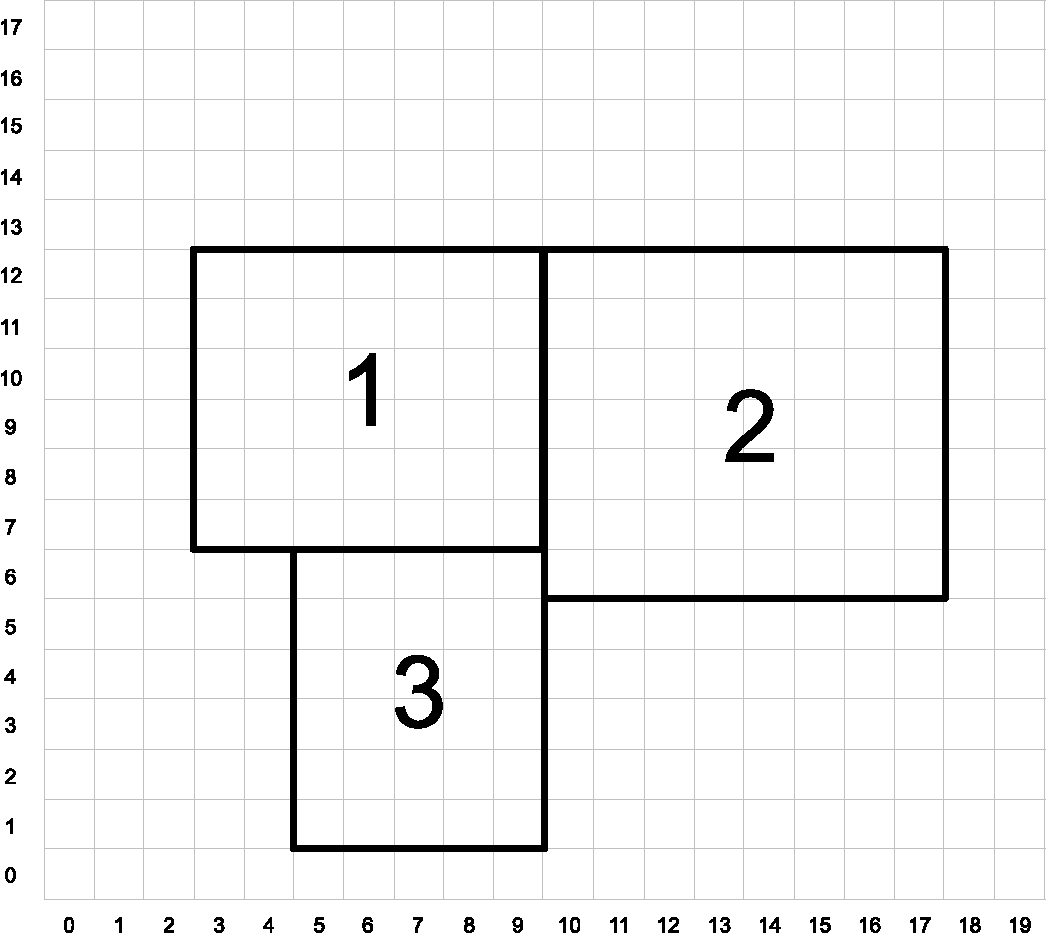
\includegraphics[width=4.0in]{index_grid2}
\caption[Single-level grid structure]
{\label{fig:soft:indexspace} Three boxes that comprise a single level.  At this
  resolution, the domain is 20$\times$18 zones.  Note that the
  indexing in BoxLib starts with $0$.}
\end{figure}




\subsection{\statedata}

\statedata\ is a class that essentially holds a pair of \multifab s: one
at the old time and one at the new time.  \boxlib\ knows how to
interpolate in time between these states to get data at any
intermediate point in time.  The main data that we care about in
\castro\ (the fluid state, gravitational potential, etc.) will be
stored as \statedata.  Essentially, data is made \statedata\ in
\castro\ if we need it to be stored in checkpoints / plotfiles, and/or
we want it to be automatically interpolated when we refine.

An {\tt AmrLevel} stores an array of \statedata.  We index this array
using integer keys (defined via an {\tt enum} in {\tt Castro.H}).  
The state data is registered with \boxlib\ in \code{Castro\_setup.cpp}.
The current \statedata\ that \castro\ carries is:
\begin{itemize}
\item {\tt State\_Type} :
\item {\tt Rad\_Type} :
\item {\tt PhiGrav\_Type} :
\item {\tt Gravity\_Type} :
\item {\tt PhiRot\_Type} :
\item {\tt Rotation\_Type} :
\item {\tt Source\_Type} :
\item {\tt LS\_State\_Type} :
\item {\tt Reactions\_Type} :
\item {\tt SDC\_Source\_Type} :
\item {\tt SDC\_React\_Type} :
\end{itemize}

We access the multifabs that carry the data of interest by interacting
with the \statedata\ using one of these keys.  For instance:
\begin{lstlisting}
MultiFab& S_new = get_new_data(State_Type);
\end{lstlisting}
gets a pointer to the multifab containing the hydrodynamics state data
at the new time.




\subsection{MFIter}

We iterate over the multifabs using an iterator {\tt MFIter}.  This
iterator knows about the locality of the data---only the boxes on the
processor will be looped over.  An example loop (for the
initialization, from {\tt Castro\_setup.cpp} would be):
\begin{lstlisting}
for (MFIter mfi(S_new); mfi.isValid(); ++mfi)
  {
     const Box& bx      = mfi.validbox();
     const int* lo      = bx.loVect();
     const int* hi      = bx.hiVect();

     if (! orig_domain.contains(bx)) {
        BL_FORT_PROC_CALL(CA_INITDATA,ca_initdata)
          (level, cur_time, lo, hi, ns,
           BL_TO_FORTRAN(S_new[mfi]), dx,
           gridloc.lo(), gridloc.hi());
     }
  }
\end{lstlisting}
Here {\tt BL\_TO\_FORTRAN} is a special \boxlib\ macro that converts the
C++ multifab into a Fortran array, and {\tt BL\_FORT\_PROC\_CALL}
is a BoxLib macro that is used to interface with Fortran routines.
{\tt ++mfi} iterates to the next FArrayBox owned by the MultiFab,
and {\tt mfi.isValid()} returns {\tt false} after we've reached
the last box contained in the MultiFab, terminating the loop.

The corresponding Fortran function will look like:
{\color{red} Need to write the Fortran version here}



\subsection{Boundaries: FillPatch and FillPatchIterator}

FillBoundary -- fills interior ghost cells for an arbitrary multifab

FillPatch works in the case that I have statedata that was defined
with ghost cells already.

FillPatchIterator works on statedata 


\subsection{Boundaries Between Grids}
Boundaries between grids are of two types. The first we call
``fine-fine'', which is two grids at the same level.  Filling ghost
cells at the same level is also part of the fillpatch operation---it's
just a straight copy from ``valid regions'' to ghost cells. The second
type is "coarse-fine", which needs interpolation from the coarse grid
to fill the fine grid ghost cells.  This also happens as part of the
FillPatch operation, which is why arrays aren't just arrays, they're
``State Data'', which means that the data knows how to interpolate
itself (in an anthropomorphical sense).  The type of interpolation to
use is defined in {\tt Castro\_setup.cpp} as well---search for
{\tt cell\_cons\_interp}, for example---that's ``cell conservative
interpolation'', i.e., the data is cell-based (as opposed to node-based
or edge-based) and the interpolation is such that the average of the
fine values created is equal to the coarse value from which they came.
(This wouldn't be the case with straight linear interpolation, for
example.)

A {\tt FillPatchIterator} is used to loop over the grids and fill
ghostcells.  One should never assume that ghostcells are valid.  A key
thing to keep in mind about the {\tt FillPatchIterator} is that you
operate on a copy of the data---the data is disconnected from the
original source.  If you want to update the data in the source,
you need to explicitly copy it back.  Also note: {\tt FillPatchIterator}
takes a multifab, but this is not filled---this is only used to
get the grid layout.  \MarginPar{did I say that right?}

{\color{red}simple example}

Basically, boundary conditions are imposed on ``state variables'' every
time that they're ``fillpatched'', as part of the fillpatch operation.

For example, the loop that calls {\tt CA\_UMDRV} (all the integration stuff) starts with
\begin{lstlisting}
   for (FillPatchIterator fpi(*this, S_new, NUM_GROW,
                              time, State_Type, strtComp, NUM_STATE);
         fpi.isValid(); ++fpi)
   {
     FArrayBox &state = fpi();

     // work on the state FAB
   }
\end{lstlisting}
Here the {\tt FillPatchIterator} is the thing that distributes the
grids over processors and makes parallel ``just work''. This fills the
single patch ``{\tt fpi}'' , which has {\tt NUM\_GROW} ghost cells,
with data of type ``{\tt State\_Type}'' at time ``{\tt time}'',
starting with component {\tt strtComp} and including a total of {\tt
  NUM\_STATE} components.

The way that you tell the code what kind of physical boundary
condition to use is given in {\tt Castro\_setup.cpp}. At the top we
define arrays such as ``{\tt scalar\_bc}'', ``{\tt norm\_vel\_bc}'',
etc, which say which kind of bc to use on which kind of physical
boundary.  Boundary conditions are set in functions like ``{\tt
  set\_scalar\_bc}'', which uses the {\tt scalar\_bc} pre-defined
arrays.

If you want to specify a value at a function (like at an inflow
boundary), there are routines in {\tt Prob\_1d.f90}, for example, which do
that. Which routine is called for which variable is again defined in
{\tt Castro\_setup.cpp}.


\subsection{pArray}



\subsection{Geometry class}

\subsection{ParmParse class}

\subsection{Derived Variables}

\subsection{Error Estimators}


\subsection{Gravity class}


\subsection{Fortran Helper Modules}

There are a number of modules that make data available to the Fortran
side of \castro\ or perform other useful tasks.

\begin{itemize}
\item {\tt prob\_params\_module}:

  This module makes the physical domain lower left and upper right
  coordinates ({\tt problo()} and {\tt probhi}) and problem center
  ({\tt center}) available.

  Here {\tt center} is the center to
  be used for the multipole expansion in gravity, certain diagnostics,
  construction of the radial velocity, etc.  It is not necessarily
  the center of the domain (e.g., for a problem modeling an octant
  of a star, it would be the origin).  This is either set by
  {\tt castro.center} or in the problem's {\tt probinit()}
  subroutine.

  This module also provides the type of physical boundary
  condition in force at each domain edge (and the integer
  keys needed to interpret them).

\item {\tt meth\_params\_module}:

  This module provides the integer keys used to access the state
  arrays for both the conserved variables ({\tt URHO}, {\tt UMX}, $\ldots$)
  and primitive variables ({\tt QRHO}, {\tt QU}, $\ldots$), as well
  as the number of scalar variables.

  It also provides the values of most of the {\tt castro.{\em xxxx}}
  runtime parameters.

\item {\tt model\_parser\_module}:

  This module is built if {\tt USE\_MODELPARSER = TRUE} is set in the
  problem's {\tt GNUmakefile}.  It then provides storage for the an
  initial model and routines to read it in and interpolate onto the
  \castro\ grid.

\item {\tt fundamental\_constants\_module}:

  This provides the CGS values of many physical constants.

\end{itemize}



\section{Setting Up Your Own Problem}

To define a new problem, we create a new directory under {\tt Exec/},
and place in it a {\tt Prob\_2d.f90} file (or {\tt 1d}/{\tt 3d},
depending on the dimensionality of the problem), a {\tt probdata.f90}
file, the {\tt inputs} and {\tt probin} files, and a {\tt
  Make.package} file that tells the build system what problem-specific
routines exist.  Finally, if you need custom boundary conditions, a
{\tt bc\_fill\_2d.f90} (or {\tt 1d}/{\tt 3d}) file is needed.  The
simplest way to get started is to copy these files from an existing
problem.  Here we describe how to customize your problem.

The purpose of these files is:
\begin{itemize}
\item \code{probdata.f90}: this holds the {\tt probdata\_module} Fortran module
  that allocates storage for all the problem-specific runtime parameters that
  are used by the problem (including those that are read from the {\tt probin}
  file.

\item \code{Prob\_?d.f90}: this holds the main routines to
  initialize the problem and grid and perform problem-specific boundary
  conditions:

  \begin{itemize}
  \item {\tt probinit()}:

    This routine is primarily responsible for reading in the {\tt
      probin} file (by defining the {\tt \&fortin} namelist and
    reading in an initial model (usually through the {\tt
      model\_parser\_module}---see the {\tt toy\_convect} problem
    setup for an example).  The parameters that are initialized
    here are those stored in the {\tt probdata\_module}.

  \item \code{ca\_initdata()}:

    This routine will initialize the state data for a single grid.
    The inputs to this routine are:
    \begin{itemize}
    \item {\tt level}: the level of refinement of the grid we are filling

    \item {\tt time}: the simulation time

    \item {\tt lo()}, {\tt hi()}: the integer indices of the box's {\em
      valid data region} lower left and upper right corners.  These
      integers refer to a global index space for the level and
      identify where in the computational domain the box lives.

    \item {\tt nscal}: the number of scalar quantities---this is not typically
      used in \castro.

    \item {\tt state\_l1}, {\tt state\_l2}, ({\tt state\_l3}): the
      integer indices of the lower left corner of the box in each
      coordinate direction.  These are for the box as allocated in memory,
      so they include any ghost cells as well as the valid data regions.

    \item {\tt state\_h1}, {\tt state\_h2}, ({\tt state\_h3}): the
      integer indices of the upper right corner of the box in each
      coordinate direction.  These are for the box as allocated in memory,
      so they include any ghost cells as well as the valid data regions.

    \item {\tt state()}: the main state array.  This is dimensioned as:
\begin{verbatim}
double precision state(state_l1:state_h1,state_l2:state_h2,NVAR)
\end{verbatim}
    (in 2-d), where {\tt NVAR} comes from the {\tt meth\_params\_module}.

    When accessing this array, we use the index keys provided by
    {\tt meth\_params\_module} (e.g., {\tt URHO}) to refer to specific
    quantities

    \item {\tt delta()}: this is an array containing the zone width ($\Delta x$)
      in each coordinate direction: $\mathtt{delta(1)} = \Delta x$,
      $\mathtt{delta(2)} = \Delta y$, $\ldots$.

    \item {\tt xlo()}, {\tt xhi()}: these are the physical coordinates of the
      lower left and upper right corners of the {\em valid region}
      of the box.  These can be used to compute the coordinates of the
      cell-centers of a zone as:
\begin{lstlisting}
  do j = lo(2), hi(2)
     y = xlo(2) + delta(2)*(dble(j-lo(2)) + 0.5d0)
     ...
\end{lstlisting}
     (Note: this method works fine for the problem initialization
     stuff, but for routines that implement tiling, as discussed below,
     {\tt lo} and {\tt xlo} may not refer to the same corner, and instead
     coordinates should be computed using {\tt problo()} from the {\tt
     prob\_params\_module}.)

    \end{itemize}
  \end{itemize}

\item \code{bc\_fill\_?d.f90}:

  These routines handle how \castro\ fills ghostcells {\em
  at physical boundaries} for specific data.  Most problem
  setups won't need to do anything special here, and inclusion
  of this file is optional -- only use it if you need to set
  specific boundary conditions.

  These routines are registered in {\tt Castro\_setup.cpp}, and
  called as needed.  By default, they just
  pass the arguments through to {\tt filcc}, which handles all of
  the generic boundary conditions (like reflecting, extrapolation,
  etc.).  The specific `{\tt fill}' routines can then supply the
  problem-specific boundary conditions, which are typically just
  Dirichlet boundary conditions (usually this means looking to see
  if the {\tt bc()} flag at a boundary is {\tt EXT\_DIR}.  The
  problem-specific code implementing these specific conditions
  should {\em follow} the {\tt filcc} call.

  \begin{itemize}
  \item {\tt ca\_hypfill}:
    This handles the boundary filling for the hyperbolic system.

  \item {\tt ca\_denfill}: At times, we need to fill just the density
    (always assumed to be the first element in the hyperbolic state)
    instead of the entire state.  When the fill patch routine is called
    with {\tt first\_comp = Density} and {\tt num\_comp = 1}, then we
    use {\tt ca\_denfill} instead of {\tt ca\_hypfill}.

    (Note: it seems that this may be used for more than just
    density, but it is only used for tagging and the plotfile)

  \item {\tt ca\_grav?fill}: These routines fill will the ghostcells
    of the gravitational acceleration grids with the gravitational
    acceleration.

    Note: for constant gravity, these routines will never be called.
    For one of the Poisson-type gravities, you only need to do
    something special here if you are implementing an {\tt Interior}
    boundary type (which you can test for by comparing {\tt
    bc(:,:,:)} to {\tt EXT\_DIR}.

    For the other standard physical boundary types, the ghost cell
    filling will be handled automatically by the default {\tt filcc}
    call in these routines.

    The gravitational acceleration in the ghost cells is used during
    the hydrodynamics portion of the code in predicting the
    interface states.

  \item {\tt ca\_reactfill}: This handles boundary filling for
    any {\tt Reactions\_Type} MultiFABs, which are sometimes used to interface
    with the nuclear burning module. It stores the normal state data
    in addition to components for the energy release and species change.

  \end{itemize}

  These routines take the following arguments:
  \begin{itemize}
  \item {\tt adv\_l1}, {\tt adv\_l2}, ({\tt adv\_l3}): the indicies of
    the lower left corner of the box holding the data we are working on.
    These indices refer to the entire box, including ghost cells.

  \item {\tt adv\_h1}, {\tt adv\_h2}, ({\tt adv\_h3}): the indicies of
    the upper right corner of the box holding the data we are working on.
    These indices refer to the entire box, including ghost cells.

  \item {\tt adv()}: the array of data whose ghost cells we are filling.
    Depending on the routine, this may have an additional index refering
    to the variable.

    This is dimensioned as:
\begin{verbatim}
  double precision adv(adv_l1:adv_h1,adv_l2:adv_h2)
\end{verbatim}

  \item {\tt domlo()}, {\tt domhi()}: the integer indices of the lower
    left and upper right corners of the valid region of the {\em entire
    domain}.  These are used to test against to see if we are filling
    physical boundary ghost cells.

    This changes according to refinement level: level-0 will
    range from {\tt 0} to {\tt castro.max\_grid\_size},
    and level-n will range from {\tt 0} to
    $\mathtt{castro.max\_grid\_size} \cdot \prod_n \mathtt{castro.ref\_ratio(n)}$.

  \item {\tt delta()}: is the zone width in each coordinate direction,
    as in {\tt initdata()} above.

  \item {\tt xlo()}: this is the physical coordinate of the lower
    left corner of the box we are filling---including the ghost cells.

    Note: this is different than how {\tt xlo()} was defined in
    {\tt initdata()} above.

  \item {\tt time}: the simulation time

  \item {\tt bc()}: an array that holds the type of boundary conditions
    to enforce at the physical boundaries for {\tt adv}.

    Sometimes it appears of the form {\tt bc(:,:)} and sometimes
    {\tt bc(:,:,:)}---the last index of the latter holds the variable
    index, i.e., density, pressure, species, etc.

    The first index is the coordinate direction and the second index
    is the domain face ({\tt 1} is low, {\tt 2} is hi), so {\tt
    bc(1,1)} is the lower $x$ boundary type, {\tt bc(1,2)} is
    the upper $x$ boundary type, {\tt bc(2,1)} is the lower
    $y$ boundary type, etc.

    To interpret the array values, we test against the quantities
    defined in {\tt bc\_types.fi} included in each subroutine,
    for example, {\tt EXT\_DIR}, {\tt FOEXTRAP}, $\ldots$.  The
    meaning of these are explained below.

  \end{itemize}

\end{itemize}


\section{Boundaries}

\subsection{Physical Boundaries}

The following boundary conditions have already been implemented in
\castro\ See {\tt BoxLib/Src/C\_AMRLib/amrlib/BC\_TYPES.H} for some
more details.
\begin{itemize}
\item {\it Outflow}:
  \begin{itemize}
    \item velocity: {\tt FOEXTRAP}
    \item temperature: {\tt FOEXTRAP}
    \item scalars: {\tt FOEXTRAP}
  \end{itemize}

\item {\it No Slip Wall with Adiabatic Temp}:
  \begin{itemize}
  \item velocity: {\tt EXT\_DIR}, $u=v=0$
  \item temperature: {\tt REFLECT\_EVEN}, $dT/dt=0$
  \item scalars: {\tt HOEXTRAP}
  \end{itemize}

\item {\it No Slip Wall with Fixed Temp}:
  \begin{itemize}
  \item velocity: {\tt EXT\_DIR}, $u=v=0$
  \item temperature: {\tt EXT\_DIR}
  \item scalars: {\tt HOEXTRAP}
  \end{itemize}

\item {\it Slip Wall with Adiabatic Temp}:
  \begin{itemize}
  \item velocity: {\tt EXT\_DIR}, $u_n=0$; {\tt HOEXTRAP}, $u_t$
  \item temperature: {\tt REFLECT\_EVEN}, $dT/dn=0$
  \item scalars: {\tt HOEXTRAP}
  \end{itemize}

\item {\it Slip Wall with Fixed Temp}:
  \begin{itemize}
  \item velocity: {\tt EXT\_DIR}, $u_n=0$
  \item temperature: {\tt EXT\_DIR}
  \item scalars: {\tt HOEXTRAP}
  \end{itemize}

\end{itemize}

Here's definitions of some of the funny-sounding ``all-caps''
words from above:
\begin{itemize}
\item {\tt INT\_DIR}: data taken from other grids or interpolated

\item {\tt EXT\_DIR}: data specified on EDGE (FACE) of bndry

\item {\tt HOEXTRAP}: higher order extrapolation to EDGE of bndry

\item {\tt FOEXTRAP}: first order extrapolation from last cell in interior

\item {\tt REFLECT\_EVEN}: $F(-n) = F(n)$ true reflection from interior cells

\item {\tt REFLECT\_ODD}: $F(-n) = -F(n)$ true reflection from interior cells
\end{itemize}


\subsection{Filling the boundaries}


\section{Parallel I/O}

Both checkpoint files and plotfiles are really directories containing
subdirectories: one subdirectory for each level of the AMR hierarchy.
The fundamental data structure we read/write to disk is a MultiFab,
which is made up of multiple FAB's, one FAB per grid.  Multiple
MultiFabs may be written to each directory in a checkpoint file.
MultiFabs of course are shared across CPUs; a single MultiFab may be
shared across thousands of CPUs.  Each CPU writes the part of the
MultiFab that it owns to disk, but they don't each write to their own
distinct file.  Instead each MultiFab is written to a runtime
configurable number of files N (N can be set in the inputs file as the
parameter \runparam{amr.checkpoint\_nfiles} and \runparam{amr.plot\_nfiles}; the
default is 64).  That is to say, each MultiFab is written to disk
across at most N files, plus a small amount of data that gets written
to a header file describing how the file is laid out in those N files.

What happens is $N$ CPUs each opens a unique one of the $N$ files into
which the MultiFab is being written, seeks to the end, and writes
their data.  The other CPUs are waiting at a barrier for those $N$
writing CPUs to finish.  This repeats for another $N$ CPUs until all the
data in the MultiFab is written to disk.  All CPUs then pass some data
to CPU {\tt 0} which writes a header file describing how the MultiFab is
laid out on disk.

We also read MultiFabs from disk in a ``chunky'' manner, opening only $N$
files for reading at a time.  The number $N$, when the MultiFabs were
written, does not have to match the number $N$ when the MultiFabs are
being read from disk.  Nor does the number of CPUs running while
reading in the MultiFab need to match the number of CPUs running when
the MultiFab was written to disk.

Think of the number $N$ as the number of independent I/O pathways in
your underlying parallel filesystem.  Of course a ``real'' parallel
filesytem should be able to handle any reasonable value of $N$.  The
value {\tt -1} forces $N$ to the number of CPUs on which you're
running, which means that each CPU writes to a unique file, which can
create a very large number of files, which can lead to inode issues.


\chapter{Single-Level Flow Chart}

\section{Overview of a single step (no SDC)}
\label{flow:sec:nosdc}

The main evolution for a single step is contained in
\code{Castro\_advance.cpp}, as \code{Castro::advance()}.  This does
the following advancement.  Note, some parts of this are only done
depending on which preprocessor directives are defined at
compile-time---the relevant directive is noted in the [\ ] at the start
of each step.

\begin{enumerate}
\item {\em Initialization} 

  This sets up the current level for advancement.  If we are at the
  start of a coarse level timestep, or we are in the middle of
  subcycling on a finer level (\code{amr\_iteration} {\tt > 1}), then
  we swap the \statedata\ from the new to old (e.g., this ensures that
  the next evolution starts with the result from the previous step).

  This also syncs up the level information to the Fortran-side of
  \castro, does any radiation initialization, and initializes all of
  the intermediate storage arrays (like those that hold source terms,
  etc.).

\item {\em Advancement} 

  This is calls \code{do\_advance} to take a single step,
  incorporating hydrodynamics, reactions, and source terms.  For
  radiation-hydrodynamics, this step does the advective (hyperbolic)
  portion of the radiation update only.

  Source terms, including gravity, rotation, and diffusion are
  included in this step, and are time-centered to achieve second-order
  accuracy.

  If \runparam{castro.use\_retry} is set, then we subcycle the current
  step if we violated any stability criteria to reach the desired
  $\Delta t$.  The idea is the following: if the timestep that you
  took had a timestep that was not sufficient to enforce the stability
  criteria that you would like to achieve, such as the CFL criterion
  for hydrodynamics or the burning stability criterion for reactions,
  you can retry the timestep by setting {\tt castro.use\_retry = 1} in
  your inputs file. This will save the current state data at the
  beginning of the level advance, and then if the criteria are not
  satisfied, will reject that advance and start over from the old
  data, with a series of subcycled timesteps that should be small
  enough to satisfy the criteria.  Note that this will effectively
  double the memory footprint on each level if you choose to use it.


\item {[\ifdef{AUX\_UPDATE}]} {\em Auxillary quantitiy evolution} 

  Auxillary variables in Castro are those that obey a continuity
  equation (with optional sources) that are passed into the EOS, but
  not subjected to the constraint on mass fractions (summing to one).

  The advection and source terms are already dealt with in the 
  main hydrodynamics advance (above step).  A user-supplied routine
  \code{ca\_auxupdate} can be provided here to further update these
  quantities.
  
\item {\em Radial data and {\rm[\ifdef{POINTMASS}]} point mass} 

  If \runparam{castro.spherical\_star} is set, then we average the state data
  over angles here to create a radial profile.  This is then used in the 
  boundary filling routines to properly set Dirichlet BCs when our domain
  is smaller than the star, so the profile on the boundaries will not 
  be uniform.

  If \runparam{castro.point\_mass\_fix\_solution} is set, then we
  change the mass of the point mass that optionally contributes to the
  gravitational potential by taking mass from the surrounding zones
  (keeping the density in those zones constant).

\item {[\ifdef{RADIATION}]} {\em Radiation implicit update} 

  The {\tt do\_advance()} routine only handled the hyperbolic
  portion of the radiation update.  This step does the implicit solve
  (either gray or multigroup) to advance the radiation energies to the 
  new time level.  Note that at the moment, this is backward-difference
  implicit (first-order in time) for stability.

  This is handled by \code{final\_radiation\_call()}.

\item {[\ifdef{PARTICLES}]} {\em Particles} 

  If we are including passively-advected particles, they are
  advanced in this step.

\item {\em Finalize}

  This cleans up the memory used during the step.  

  If \runparam{castro.track\_grid\_losses} is set, then we also add up
  the mass that left through the boundary over this
  step.\footnote{Note: this functionality assumes that only the
    coarse grid touches the physical boundary.  It does not use any
    use masks to prevent double counting if multiple levels touch
    the boundary.}

\end{enumerate}

\subsection{Main Hydro, Reaction, and Gravity Advancement (Strang-splitting)}

The explicit portion of the system advancement (reactions,
hydrodynamics, and gravity) is done by \code{do\_advance()}.  Consider
our system of equations as:
\begin{equation}
\frac{\partial\Ub}{\partial t} = \nabla\cdot\Fb + \Rb(\Ub) + \Sb,
\end{equation}
where $\Fb$ is the flux vector, $\Rb$ are the reaction
source terms, and $\Sb$ are the non-reaction source terms, which
includes any user-defined external sources, $\Sb_{\rm ext}$.  We use
Strang splitting to discretize the advection-reaction equations.  In
summary, for each time step, we update the conservative variables,
$\Ub$, by reacting for half a time step, advecting for a full time
step (ignoring the reaction terms), and reacting for half a time step.
The treatment of source terms complicates this a little.  The actual
update, in sequence, looks like:
\begin{align}
\Ub^\star &= \Ub^n + \frac{\dt}{2}\Rb(\Ub^n) \\
\Ub^{n+1,(a)} &= \Ub^\star + \dt\, \Sb(\Ub^\star) \\
\Ub^{n+1,(b)} &= \Ub^{n+1,(a)} - \dt\, {\bf A}(\Ub^\star) \\
\Ub^{n+1,(c)} &= \Ub^{n+1,(b)} + \frac{\dt}{2}\, [\Sb(\Ub^{n+1,(b)}) - \Sb(\Ub^\star)] \label{eq:source_correct}\\
\Ub^{n+1}     &= \Ub^{n+1,(c)} + \frac{\dt}{2} \Rb(\Ub^{n+1,(c)})
\end{align}
Note that in the first step, we add a full $\Delta t$ of the old-time
source to the state.  This prediction ensures consistency when it
comes time to predicting the new-time source at the end of the update.
The construction of the advective terms, ${\bf A(\Ub)}$ is purely
explicit, and based on an unsplit second-order Godunov method.  We
predict the standard primitive variables, as well as $\rho e$, at
time-centered edges and use an approximate Riemann solver construct
fluxes.

At the beginning of the time step, we assume that $\Ub$ and $\phi$ are
defined consistently, i.e., $\rho^n$ and $\phi^n$ satisfy equation
(\ref{eq:Self Gravity}).  Also note that in
Eq.~\ref{eq:source_correct}, we actually can do the new time-level
source updates in sequence (this is the default, and is controlled by
\runparam{castro.update\_state\_between\_sources}.  Additionally, some
terms, like rotation, can be treated implicitly.  Together, this can
make the update more akin to:
\begin{equation}
\Ub^{n+1,(c)} = \Ub^{n+1,(b)} + \frac{\dt}{2} [\Sb(\Ub^{n+1,(c)}) - \Sb(\Ub^n)]
\end{equation}

\castro\ also supports radiation.  This part of the update algorithm
only deals with the advective / hyperbolic terms in the radiation update.

Here is the single-level algorithm.  In the code, the objective is to
evolve the state from the old time, {\tt S\_old}, to the new time,
{\tt S\_new}.  \MarginPar{Sborder?}

\begin{enumerate}
\item \label{strang:init} {\em Initialize} [\code{initialize\_do\_advance()}]

  This resets the flux registers and initializes a lot of intermediate
  storage arrays (like source term) to zero.

  We also check for NaNs in the initial state, {\tt S\_old}.

\item {\em React $\Delta t/2$.} [\code{strang\_react\_first\_half()}]

  Update the solution due to the effect of reactions over half a time
  step.  The integration method and system of equations used here is
  determined by a host of runtime parameters that are part of the
  \microphysics\ package.  But the basic idea is to evolve the energy
  release from the reactions, the species mass fractions, and
  temperature through $\Delta t/2$.

  Using the notation above, we begin with the time-level $n$ state,
  $\Ub^n$, and produce a state that has evolved only due to reactions,
  $\Ub^\star$.

  \begin{align}
    (\rho e)^\star &= (\rho e)^\star - \frac{\dt}{2} \rho H_\mathrm{nuc} \\
    (\rho E)^\star &= (\rho E)^\star - \frac{\dt}{2} \rho H_\mathrm{nuc} \\
    (\rho X_k)^\star &= (\rho X_k)^\star + \frac{\dt}{2}(\rho\omegadot_k)^n.
  \end{align}
  Here, $H_\mathrm{nuc}$ is the energy release (erg/g/s) over the
  burn, and $\omegadot_k$ is the creation rate for species $k$.

  After exiting the burner, we call the EOS with $\rho^\star$,
  $e^\star$, and $X_k^\star$ to get the new temperature, $T^\star$.

  Note that the density, $\rho$, does not change via reactions in the
  Strang-split formulation.

  The reaction data needs to be valid in the ghost cells.  The logic
  in this routine (accomplished throuh the use of a mask) will burn
  only in the valid interior cells or in any ghost cells that are on a
  coarse-fine interface or physical boundary\MarginPar{physical
    boundary too?}  This allows us to just use a level {\tt
    FillBoundary} call to fill all of the ghost cells on the same
  level with valid data.

  An experimental option (enabled via
  \runparam{use\_custom\_knapsack\_weights}) will create a custom
  distribution map based on the work needed in burning a zone and
  redistribute the boxes across processors before burning, to better
  load balance..  \MarginPar{need to explain the logic here,
    especially what the parallel copies are doing}


\item \label{strang:oldsource} {\em Construct time-level $n$ sources and apply} 
  [\code{construct\_old\_gravity()}, \code{do\_old\_sources()}]

  The time level $n$ sources are computed, stored in the appropriate
  \multifab\ in \variable{old\_sources}, and applied to the state
  after the burn, $\Ub^\star$ with a full $\Delta t$ weighting (this
  will be corrected later).  This produces the intermediate state,
  $\Ub^{n+1,(a)}$.

  The sources that we deal with here are:
  \begin{enumerate}
  \item sponge : the sponge\index{sponge} is a damping term added to
    the momentum equation that is designed to drive the velocities to
    zero over some timescale.  Our implementation of the sponge
    follows that of \maestro~\cite{maestro:III}

  \item external sources : users can define problem-specific sources
    in the \code{ext\_src\_?d.f90} file.  Sources for the different
    equations in the conservative state vector, $\Ub$, are indexed
    using the integer keys defined in {\tt meth\_params\_module}
    (e.g., {\tt URHO}).

    This is most commonly used for external heat sources (see the
    \problem{toy\_convect} problem setup) for an example.  But most
    problems will not use this.

  \item {[\ifdef{DIFFUSION}]} diffusion : thermal diffusion can be
    added in an explicit formulation.  Second-order accuracy is
    achieved by averaging the time-level $n$ and $n+1$ terms, using
    the same predictor-corrector strategy described here.

    Note: thermal diffusion is distinct from radiation hydrodynamics.

    Also note that incorporating diffusion brings in an additional
    timestep constraint, since the treatment is explicit.  See
    Chapter~\ref{ch:diffusion} for more details. 

  \item {[\ifdef{HYBRID\_MOMENTUM}]} angular momentum 

    \MarginPar{need to write this up}

  \item {[\ifdef{GRAVITY}]} gravity:

    For full Poisson gravity, we solve for for gravity using:
    \begin{equation}
      \gb^n = -\nabla\phi^n, \qquad
      \Delta\phi^n = 4\pi G\rho^n,
    \end{equation}

    The construction of the form of the gravity source for the
    momentum and energy equation is dependent on the parameter
    \runparam{castro.grav\_source\_type}.  Full details of the gravity
    solver are given in Chapter~\ref{ch:gravity}.

    \MarginPar{we should add a description of whether we do a level solve or a composite solve}

    \MarginPar{what do we store? phi and g? source?}

  \item {[\ifdef{ROTATION}]} rotation

    We compute the rotational potential (for use in the energy update)
    and the rotational acceleration (for use in the momentum
    equation).  This includes the Coriolis and centrifugal terms in a
    constant-angular-velocity co-rotating frame.  The form of the
    rotational source that is constructed then depends on the
    parameter \runparam{castro.rot\_source\_type}.  More details are
    given in Chapter~\ref{ch:rotation}.
    
  \end{enumerate}

  The source terms here are evaluated using the post-burn state,
  $\Ub^\star$, and later corrected by using the new state just before
  the burn, $\Ub^{n+1,(b)}$.  This is compatible with
  Strang-splitting, since the hydro and sources takes place completely
  inside of the surrounding burn operations.

\item \label{strang:hydro} {\em Construct the hydro update} [\code{construct\_hydro\_source()}]

  The goal is to advance our system considering only the advective
  terms (which in Cartesian coordinates can be written as the
  divergence of a flux).

  We do the hydro update in two parts---first we construct the
  advective update and store it in the \variable{hydro\_source}
  \multifab, then we do the conservative update in a separate step.  This
  separation allows us to use the advective update separately in more
  complex time-integration schemes.

  In the Strang-split formulation, we start the reconstruction using
  the state after burning, $\Ub^\star$, and predict to the half-time
  ($n+1/2$) to get a second-order accurate method.  The advection step
  is complicated, and more detail is given in Section
  \ref{Sec:Advection Step}.  Here is the summarized version:
  \begin{enumerate}
  \item Compute primitive variables.
  \item Convert the source terms to those acting on primitive variables
  \item Predict primitive variables to time-centered edges.
  \item Solve the Riemann problem.
  \item Compute fluxes and update.
  \end{enumerate}

  To start the hydrodynamics, we need to know the hydrodynamics source
  terms at time-level $n$, since this enters into the prediction to
  the interface states.  This is essentially the same vector that was
  computed in the previous step, with a few modifications.  The most
  important is that if we set
  \runparam{castro.source\_term\_predictor}, then we extrapolate the
  source terms from $n$ to $n+1/2$, using the change from the previous
  step.

  Note: we neglect the reaction source terms, since those are already
  accounted for in the state directly, due to the Strang-splitting
  nature of this method.


\item \label{strang:radial} {\em Update radial data and center of mass for monopole gravity}
 \MarginPar{is that right?}


\item \label{strang:clean} {\em Clean State} [\code{clean\_state()}]

  There are many ways that the hydrodynamics state may become
  unphysical in the evolution.  The \code{clean\_state()} routine
  enforces some checks on the state.  In particular, it
  \begin{enumerate}
  \item enforces that the density is above \runparam{castro.small\_dens}
  \item normalizes the species so that the mass fractions sum to 1
  \item resets the internal energy and temperature to 
    make them consistent with the total energy
  \end{enumerate}

  After these checks, we check the state for NaNs.


\item \label{strang:newsource} {\em Correct the source terms with the $n+1$ contribution}
  [\code{construct\_new\_gravity()}, \code{do\_new\_sources}]

  Previously we added $\Delta t\, \Sb(\Ub^\star)$ to the state, when
  we really want a time-centered approach, $(\Delta t/2)[\Sb(\Ub^\star
    + \Sb(\Ub^{n+1,(b)})]$.  We fix that here.

  We start by computing the source term vector $\Sb(\Ub^{n+1,(b)})$
  using the updated state, $\Ub^{n+1,(b)}$.  We then compute the
  correction, $(\Delta t/2)[\Sb(\Ub^{n+1,(b)}) - \Sb(\Ub^\star)]$ to
  add to $\Ub^{n+1,(b)}$ to give us the properly time-centered source,
  and the fully updated state, $\Ub^{n+1,(c)}$.  This correction is stored
  in the \variable{new\_sources} \multifab\footnote{The correction for gravity is slightly different since we directly compute the time-centered gravitational source term using the hydrodynamic fluxes.}.

  We have a choice of how to do this correction.  We can first compute
  all the corrections using the same initial state, $U^{n+1,(b)}$,
  and then apply them all.  Or we can compute them one-by-one applying
  them as we go.  This behavior is controlled by the parameter
  \runparam{castro.update\_state\_between\_sources}.

  In the process of updating the sources, we update the temperature to
  make it consistent with the new state.

%% We need to correct the solution by effectively time-centering the
%% source terms.  These corrections are to be performed sequentially
%% since new source term evaluations may depend on previous corrections.

%% First, we correct the solution with the updated gravity:
%% \begin{eqnarray}
%% (\rho\ub)^{n+1} &=& (\rho\ub)^{n+1} + \frac{\dt}{2}\left[(\rho\gb)^{n+1} - (\rho\gb)^n\right], \\
%% (\rho E)^{n+1} &=& (\rho E)^{n+1} + \frac{\dt}{2}\left[\left(\rho\ub\cdot\gb\right)^{n+1} - \left(\rho\ub\cdot\gb\right)^n\right].
%% \end{eqnarray}

%% Next, we correct $\Ub$ with updated external sources.  For example,
%% for the momentum, we correct using
%% \begin{equation}
%% (\rho\ub)^{n+1} = (\rho\ub)^{n+1} + \frac{\dt}{2}\left(\Sb_{{\rm ext},\rho\ub}^{n+1} - \Sb_{{\rm ext},\rho\ub}^n\right).
%% \end{equation}
%% We correct $\rho E, \rho A_k, \rho X_k$, and $\rho Y_k$ in an
%% analogous manner.

%% Finally, we correct the solution with updated thermal diffusion using
%% \begin{equation}
%% (\rho E)^{n+1} = (\rho E)^{n+1} + \frac{\dt}{2}\left(\nabla\cdot\kappa\nabla T^{n+1} - \nabla\cdot\kappa\nabla T^n\right).
%% \end{equation}


\item {\em React $\Delta t/2$.} [\code{strang\_react\_second\_half()}]

  We do the final $\dt/2$ reacting on the state, begining with $\Ub^{n+1,(c)}$ to
  give us the final state on this level, $\Ub^{n+1}$.

  This is largely the same as \code{strang\_react\_first\_half()}, but
  it does not currently fill the reactions in the ghost cells. \MarginPar{confirm this}

\item \label{strang:finalize} {\em Finalize} [\code{finalize\_do\_advance()}]

  Finalize does the following:
  \begin{enumerate}
  \item for the momentum sources, we compute $d\Sb/dt$, to use in the
    source term prediction/extrapolation for the hydrodynamic
    interface states during the next step.

  \item If we are doing the hybrid momentum algorithm, then we sync up
    the hybrid and linear momenta
  \end{enumerate}

\end{enumerate}


\section{Overview of a single step (with SDC)}

We express our system as:
\begin{equation}
\Ub_t = \mathcal{A}(\Ub) + \Rb(\Ub)
\end{equation}
here $\mathcal{A}$ is the advective source, which includes both the 
flux divergence and the hydrodynamic source terms (e.g.\ gravity):
\begin{equation}
\mathcal{A}(\Ub) = -\nabla \cdot \Fb(\Ub) + \Sb
\end{equation}

The SDC version of the main advance loop looks similar to the no-SDC
version, but includes an iteration loop over the hydro, gravity, and
reaction update.  So the only difference happens in step 2 of the
flowchart outlined in \S~\ref{flow:sec:nosdc}.  In particular this
step now proceeds as:

\begin{enumerate}
\setcounter{enumi}{1}

\item {\em Advancement}

  Loop $k$ from 0 to {\tt sdc\_iters}, doing:

  \begin{enumerate}
    \item {\em Hydrodynamics advance}: This is done through {\tt
      do\_advance}---in SDC mode, this only updates the hydrodynamics,
      including the non-reacting sources.  However, in predicting the
      interface states, we use an iteratively-lagged approximation to the 
      reaction source on the primitive variables, $\mathcal{I}_q^{k-1}$.  \MarginPar{first time through is this source 0?}

      The result of this is an approximation to $\mathcal{A}(\Ub)$,
      stored in \variable{hydro\_sources} (the flux divergence)
      and \variable{old\_sources} and \variable{new\_sources}.

    \item {\em React}: Reactions are integrated with the advective
      update as a source---this way the reactions see the
      time-evolution due to advection as we integrate:
      \begin{equation}
        \frac{d\Ub}{dt} = \left [ \mathcal{A}(\Ub) \right ]^{n+1/2} + \Rb(\Ub)
      \end{equation}
     The advective source includes both the divergence of the fluxes
      as well as the time-centered source terms.  This is computed by
      \code{sum\_of\_sources()} by summing over all source components
      \variable{hydro\_source}, \variable{old\_sources}, and
      \variable{new\_sources}.  

    \item {\em Clean state}: This ensures that the thermodynamic state is
      valid and consistent.

    \item {\em Construct reaction source terms}: Construct the change
      in the primitive variables due only to reactions over the
      timestep, $\mathcal{I}_q^{k}$.  This will be used in the next
      iteration.
  \end{enumerate}


\end{enumerate}


Note that is it likely that some of the other updates (like any
non-advective auxillary quantity updates) should be inside the SDC
loop, but presently they are only done at the end.  Also note that the
radiation implicit update is not done as part of the SDC iterations.


\subsection{Main Hydro and Gravity Advancement (SDC)}

The evolution in {\tt do\_advance} is substantially different than the
Strang case.  In particular, reactions are not evolved.  Here we
summarize those differences.

\begin{enumerate}
\item {\em Initialize} [\code{initialize\_do\_advance()}]

This is unchanged from step \ref{strang:init} in the Strang algorithm.


\item {\em Construct time-level $n$ sources and apply} 
  [\code{construct\_old\_gravity()}, \code{do\_old\_sources()}]

This corresponds to step \ref{strang:oldsource} in the Strang
algorithm.  There are not differences compared to the Strang
algorithm, although we note, this only needs to be done for the first
SDC iteration in the advancement, since the old state does not change.\MarginPar{we need to fix the code to only do this once}

\item {\em Construct the hydro update} [\code{construct\_hydro\_source()}]

This corresponds to step~\ref{strang:hydro} in the Strang
algorithm.  There are a few major differences with the Strang case:
\begin{itemize}
\item There is no need to extrapolate source terms to the half-time
  for the prediction (the \runparam{castro.source\_term\_predictor}
  parameter), since SDC provides a natural way to approximate the
  time-centered source---we simply use the iteratively-lagged new-time
  source.

\item The primitive variable source terms that are used for the
  prediction include the contribution due to reactions (from the last
  SDC iteration).  This addition is done in
  \code{construct\_hydro\_source()} after the source terms are
  converted to primitive variables.
\end{itemize}

\item {\em Update radial data and center of mass for monopole gravity}
  
  This is the same as the Strang step~\ref{strang:radial}


\item {\em Clean State} [\code{clean\_state()}]

  This is the same as the Strang step~\ref{strang:clean}

\item \label{strang:newsource} {\em Correct the source terms with the $n+1$ contribution}
  [\code{construct\_new\_gravity()}, \code{do\_new\_sources}]

  This is the same as the Strang step~\ref{strang:newsource}

\item {\em Finalize} [\code{finalize\_do\_advance()}]

  This differs from Strang step~\ref{strang:finalize} in that we do not
  construct $d\Sb/dt$, but instead store the total hydrodynamical source
  term at the new time.  As discussed above, this will be used in the 
  next iteration to approximate the time-centered source term.

\end{enumerate}






\chapter{Runtime Parameters}
\label{chapter:parameters}

\section{Introduction to Runtime Parameters}

The behavior of the network and EOS are controlled by many runtime
parameters.  These parameters are defined in plain-text files {\tt
  \_parameters} located in the different directories that hold the
microphysics code.  At compile time, a script in the \boxlib\ bulid
system, {\tt findparams.py}, locates all of the {\tt \_parameters}
files that are needed for the given choice of network, integrator, and
EOS, and assembles all of the runtime parameters into a module named
{\tt extern\_probin\_module} (using the {\tt write\_probin.py}
script).  

Note: depending on the application code, the filename of the source 
file that contains the {\tt extern\_probin\_module} may differ
(in \castro\ it is {\tt extern.f90}, and uses the {\tt \&extern} namelist;
in \maestro\ it is in the main {\tt probin.f90} and uses the same namelist
as general \maestro\ runtime parameters).

Parameter definitions take the form of:
\begin{verbatim}
# comment describing the parameter
name              data-type       default-value      priority
\end{verbatim}
Here, the {\tt priority} is simply an integer.  When two directories
define the same parameter, but with different defaults, the version of
the parameter with the highest priority takes precedence.  This allows
specific implementations to override the general parameter defaults.

The documentation below is automatically generated, using the comments
in the {\tt \_parameters} files.



\section{Removed Runtime Parameters}

The following runtime parameters have been removed for \castro.
\begin{itemize}
\item {\tt castro.ppm\_flatten\_before\_integrals} : this parameter
  controlled whether we applied the flattening of the parabolic
  profiles before we integrated under their profiles or afterwards.
  The default was switched to flattening before the integration,
  which is more consistent with the original PPM methodology.  This
  parameter was removed since the variation enabled by this parameter
  was not that great.
\end{itemize}


\section{ {\tt castro } Namespace}

\label{ch:parameters}


%%%%%%%%%%%%%%%%
% symbol table
%%%%%%%%%%%%%%%%

\begin{landscape}


{\small

\renewcommand{\arraystretch}{1.5}
%
\begin{center}
\begin{longtable}{|l|p{5.25in}|l|}
\caption[castro :  AMR
 parameters]{castro :  AMR
 parameters} \label{table: castro :  AMR
 parameters runtime} \\
%
\hline \multicolumn{1}{|c|}{\textbf{parameter}} & 
       \multicolumn{1}{ c|}{\textbf{description}} & 
       \multicolumn{1}{ c|}{\textbf{default value}} \\ \hline 
\endfirsthead

\multicolumn{3}{c}%
{{\tablename\ \thetable{}---continued}} \\
\hline \multicolumn{1}{|c|}{\textbf{parameter}} & 
       \multicolumn{1}{ c|}{\textbf{description}} & 
       \multicolumn{1}{ c|}{\textbf{default value}} \\ \hline 
\endhead

\multicolumn{3}{|r|}{{\em continued on next page}} \\ \hline
\endfoot

\hline 
\endlastfoot


\rowcolor{tableShade}
\runparamNS{do\_reflux}{castro} &  do we do the hyperbolic reflux at coarse-fine interfaces? & 1 \\
\runparamNS{lin\_limit\_state\_interp}{castro} &  how to do limiting of the state data when interpolating 0: only prevent new extrema 1: preserve linear combinations of state variables & 0 \\
\rowcolor{tableShade}
\runparamNS{state\_interp\_order}{castro} &  highest order used in interpolation & 1 \\
\runparamNS{state\_nghost}{castro} &  Number of ghost zones for state data to have. Note that if you are using radiation, choosing this to be zero will be overridden since radiation needs at least one ghost zone. & 0 \\
\rowcolor{tableShade}
\runparamNS{update\_sources\_after\_reflux}{castro} &  whether to re-compute new-time source terms after a reflux & 1 \\
\runparamNS{use\_custom\_knapsack\_weights}{castro} &  should we have state data for custom load-balancing weighting? & 0 \\


\end{longtable}
\end{center}

} % ends \small


{\small

\renewcommand{\arraystretch}{1.5}
%
\begin{center}
\begin{longtable}{|l|p{5.25in}|l|}
\caption[castro :  diagnostics, I/O
 parameters]{castro :  diagnostics, I/O
 parameters} \label{table: castro :  diagnostics, I/O
 parameters runtime} \\
%
\hline \multicolumn{1}{|c|}{\textbf{parameter}} & 
       \multicolumn{1}{ c|}{\textbf{description}} & 
       \multicolumn{1}{ c|}{\textbf{default value}} \\ \hline 
\endfirsthead

\multicolumn{3}{c}%
{{\tablename\ \thetable{}---continued}} \\
\hline \multicolumn{1}{|c|}{\textbf{parameter}} & 
       \multicolumn{1}{ c|}{\textbf{description}} & 
       \multicolumn{1}{ c|}{\textbf{default value}} \\ \hline 
\endhead

\multicolumn{3}{|r|}{{\em continued on next page}} \\ \hline
\endfoot

\hline 
\endlastfoot


\rowcolor{tableShade}
\runparamNS{hard\_cfl\_limit}{castro} &  abort if we exceed CFL = 1 over the cource of a timestep & 1 \\
\runparamNS{job\_name}{castro} &  a string describing the simulation that will be copied into the plotfile's {\tt job\_info} file & "" \\
\rowcolor{tableShade}
\runparamNS{output\_at\_completion}{castro} &  write a final plotfile and checkpoint upon completion & 1 \\
\runparamNS{print\_fortran\_warnings}{castro} &  display warnings in Fortran90 routines & (0, 1) \\
\rowcolor{tableShade}
\runparamNS{print\_update\_diagnostics}{castro} &  display information about updates to the state (how much mass, momentum, energy added) & (0, 1) \\
\runparamNS{reset\_checkpoint\_step}{castro} &  Do we want to reset the number of steps in the checkpoint? This ONLY takes effect if amr.regrid\_on\_restart = 1 and amr.checkpoint\_on\_restart = 1, (which require that max\_step and stop\_time be less than the value in the checkpoint) and you set it to value greater than this default value. & -1 \\
\rowcolor{tableShade}
\runparamNS{reset\_checkpoint\_time}{castro} &  Do we want to reset the time in the checkpoint? This ONLY takes effect if amr.regrid\_on\_restart = 1 and amr.checkpoint\_on\_restart = 1, (which require that max\_step and stop\_time be less than the value in the checkpoint) and you set it to value greater than this default value. & -1.e200 \\
\runparamNS{show\_center\_of\_mass}{castro} &  display center of mass diagnostics & 0 \\
\rowcolor{tableShade}
\runparamNS{sum\_interval}{castro} &  how often (number of coarse timesteps) to compute integral sums (for runtime diagnostics) & -1 \\
\runparamNS{sum\_per}{castro} &  how often (simulation time) to compute integral sums (for runtime diagnostics) & -1.0e0 \\
\rowcolor{tableShade}
\runparamNS{track\_grid\_losses}{castro} &  calculate losses of material through physical grid boundaries & 0 \\


\end{longtable}
\end{center}

} % ends \small


{\small

\renewcommand{\arraystretch}{1.5}
%
\begin{center}
\begin{longtable}{|l|p{5.25in}|l|}
\caption[castro :  diffusion
 parameters]{castro :  diffusion
 parameters} \label{table: castro :  diffusion
 parameters runtime} \\
%
\hline \multicolumn{1}{|c|}{\textbf{parameter}} & 
       \multicolumn{1}{ c|}{\textbf{description}} & 
       \multicolumn{1}{ c|}{\textbf{default value}} \\ \hline 
\endfirsthead

\multicolumn{3}{c}%
{{\tablename\ \thetable{}---continued}} \\
\hline \multicolumn{1}{|c|}{\textbf{parameter}} & 
       \multicolumn{1}{ c|}{\textbf{description}} & 
       \multicolumn{1}{ c|}{\textbf{default value}} \\ \hline 
\endhead

\multicolumn{3}{|r|}{{\em continued on next page}} \\ \hline
\endfoot

\hline 
\endlastfoot


\rowcolor{tableShade}
\runparamNS{diffuse\_cond\_scale\_fac}{castro} &  scaling factor for conductivity & 1.0 \\
\runparamNS{diffuse\_cutoff\_density}{castro} &  set a cutoff density for diffusion -- we zero the term out below this density & -1.e200 \\
\rowcolor{tableShade}
\runparamNS{diffuse\_enth}{castro} &  enable enthalpy diffusion & 0 \\
\runparamNS{diffuse\_spec}{castro} &  enable species diffusion & 0 \\
\rowcolor{tableShade}
\runparamNS{diffuse\_temp}{castro} &  enable thermal diffusion & 0 \\
\runparamNS{diffuse\_vel}{castro} &  enable velocity diffusion & 0 \\


\end{longtable}
\end{center}

} % ends \small


{\small

\renewcommand{\arraystretch}{1.5}
%
\begin{center}
\begin{longtable}{|l|p{5.25in}|l|}
\caption[castro :  embiggening
 parameters]{castro :  embiggening
 parameters} \label{table: castro :  embiggening
 parameters runtime} \\
%
\hline \multicolumn{1}{|c|}{\textbf{parameter}} & 
       \multicolumn{1}{ c|}{\textbf{description}} & 
       \multicolumn{1}{ c|}{\textbf{default value}} \\ \hline 
\endfirsthead

\multicolumn{3}{c}%
{{\tablename\ \thetable{}---continued}} \\
\hline \multicolumn{1}{|c|}{\textbf{parameter}} & 
       \multicolumn{1}{ c|}{\textbf{description}} & 
       \multicolumn{1}{ c|}{\textbf{default value}} \\ \hline 
\endhead

\multicolumn{3}{|r|}{{\em continued on next page}} \\ \hline
\endfoot

\hline 
\endlastfoot


\rowcolor{tableShade}
\runparamNS{grown\_factor}{castro} &  the factor by which to extend the domain upon restart for embiggening & 1 \\
\runparamNS{star\_at\_center}{castro} &  used with the embiggening routines to determine how to extend the domain & -1 \\


\end{longtable}
\end{center}

} % ends \small


{\small

\renewcommand{\arraystretch}{1.5}
%
\begin{center}
\begin{longtable}{|l|p{5.25in}|l|}
\caption[castro :  gravity and rotation
 parameters]{castro :  gravity and rotation
 parameters} \label{table: castro :  gravity and rotation
 parameters runtime} \\
%
\hline \multicolumn{1}{|c|}{\textbf{parameter}} & 
       \multicolumn{1}{ c|}{\textbf{description}} & 
       \multicolumn{1}{ c|}{\textbf{default value}} \\ \hline 
\endfirsthead

\multicolumn{3}{c}%
{{\tablename\ \thetable{}---continued}} \\
\hline \multicolumn{1}{|c|}{\textbf{parameter}} & 
       \multicolumn{1}{ c|}{\textbf{description}} & 
       \multicolumn{1}{ c|}{\textbf{default value}} \\ \hline 
\endhead

\multicolumn{3}{|r|}{{\em continued on next page}} \\ \hline
\endfoot

\hline 
\endlastfoot


\rowcolor{tableShade}
\runparamNS{do\_grav}{castro} &  permits gravity calculation to be turned on and off & -1 \\
\runparamNS{do\_rotation}{castro} &  permits rotation calculation to be turned on and off & -1 \\
\rowcolor{tableShade}
\runparamNS{grav\_source\_type}{castro} &  determines how the gravitational source term is added to the momentum and energy state variables. & 4 \\
\runparamNS{implicit\_rotation\_update}{castro} &  we can do a implicit solution of the rotation update to allow for better coupling of the Coriolis terms & 1 \\
\rowcolor{tableShade}
\runparamNS{moving\_center}{castro} &  to we recompute the center used for the multipole gravity solve each step? & 0 \\
\runparamNS{point\_mass}{castro} &  mass of the point mass & 0.0 \\
\rowcolor{tableShade}
\runparamNS{point\_mass\_fix\_solution}{castro} &  if we have a central point mass, we can prevent mass from building up in the zones adjacent to it by keeping their density constant and adding their mass to the point mass object & 0 \\
\runparamNS{rot\_axis}{castro} &  the coordinate axis ($x=1$, $y=2$, $z=3$) for the rotation vector & 3 \\
\rowcolor{tableShade}
\runparamNS{rot\_source\_type}{castro} &  determines how the rotation source terms are added to the momentum and energy equations & 4 \\
\runparamNS{rotation\_include\_centrifugal}{castro} &  permits the centrifugal terms in the rotation to be turned on and off & 1 \\
\rowcolor{tableShade}
\runparamNS{rotation\_include\_coriolis}{castro} &  permits the Coriolis terms in the rotation to be turned on and off & 1 \\
\runparamNS{rotation\_include\_domegadt}{castro} &  permits the d(omega)/dt terms in the rotation to be turned on and off & 1 \\
\rowcolor{tableShade}
\runparamNS{rotational\_dPdt}{castro} &  the rotation periods time evolution---this allows the rotation rate to change durning the simulation time & 0.0 \\
\runparamNS{rotational\_period}{castro} &  the rotation period for the corotating frame & -1.e200 \\
\rowcolor{tableShade}
\runparamNS{state\_in\_rotating\_frame}{castro} &  Which reference frame to measure the state variables with respect to. The standard in the literature when using a rotating reference frame is to measure the state variables with respect to an observer fixed in that rotating frame. If this option is disabled by setting it to 0, the state variables will be measured with respect to an observer fixed in the inertial frame (but the frame will still rotate). & 1 \\
\runparamNS{use\_point\_mass}{castro} &  include a central point mass & 1 \\


\end{longtable}
\end{center}

} % ends \small


{\small

\renewcommand{\arraystretch}{1.5}
%
\begin{center}
\begin{longtable}{|l|p{5.25in}|l|}
\caption[castro :  hydrodynamics
 parameters]{castro :  hydrodynamics
 parameters} \label{table: castro :  hydrodynamics
 parameters runtime} \\
%
\hline \multicolumn{1}{|c|}{\textbf{parameter}} & 
       \multicolumn{1}{ c|}{\textbf{description}} & 
       \multicolumn{1}{ c|}{\textbf{default value}} \\ \hline 
\endfirsthead

\multicolumn{3}{c}%
{{\tablename\ \thetable{}---continued}} \\
\hline \multicolumn{1}{|c|}{\textbf{parameter}} & 
       \multicolumn{1}{ c|}{\textbf{description}} & 
       \multicolumn{1}{ c|}{\textbf{default value}} \\ \hline 
\endhead

\multicolumn{3}{|r|}{{\em continued on next page}} \\ \hline
\endfoot

\hline 
\endlastfoot


\rowcolor{tableShade}
\runparamNS{add\_ext\_src}{castro} &  if true, define an additional source term & 0 \\
\runparamNS{allow\_negative\_energy}{castro} &  Whether or not to allow internal energy to be less than zero & 0 \\
\rowcolor{tableShade}
\runparamNS{allow\_small\_energy}{castro} &  Whether or not to allow the internal energy to be less than the internal energy corresponding to small\_temp & 1 \\
\runparamNS{cg\_blend}{castro} &  for the Colella \& Glaz Riemann solver, what to do if we do not converge to a solution for the star state. 0 = do nothing; print iterations and exit 1 = revert to the original guess for p-star 2 = do a bisection search for another 2 * cg\_maxiter iterations. & 2 \\
\rowcolor{tableShade}
\runparamNS{cg\_maxiter}{castro} &  for the Colella \& Glaz Riemann solver, the maximum number of iterations to take when solving for the star state & 12 \\
\runparamNS{cg\_tol}{castro} &  for the Colella \& Glaz Riemann solver, the tolerance to demand in finding the star state & 1.0e-5 \\
\rowcolor{tableShade}
\runparamNS{density\_reset\_method}{castro} &  Which method to use when resetting a negative/small density 1 = Reset to characteristics of adjacent zone with largest density 2 = Use average of all adjacent zones for all state variables 3 = Reset to the original zone state before the hydro update & 1 \\
\runparamNS{difmag}{castro} &  the coefficient of the artificial viscosity & 0.1 \\
\rowcolor{tableShade}
\runparamNS{do\_ctu}{castro} &  do we do the CTU unsplit method or a method-of-lines approach? & 1 \\
\runparamNS{do\_hydro}{castro} &  permits hydro to be turned on and off for running pure rad problems & -1 \\
\rowcolor{tableShade}
\runparamNS{do\_sponge}{castro} &  permits sponge to be turned on and off & 0 \\
\runparamNS{dual\_energy\_eta1}{castro} &  Threshold value of (E - K) / E such that above eta1, the hydrodynamic pressure is derived from E - K; otherwise, we use the internal energy variable UEINT. & 1.0e0 \\
\rowcolor{tableShade}
\runparamNS{dual\_energy\_eta2}{castro} &  Threshold value of (E - K) / E such that above eta2, we update the internal energy variable UEINT to match E - K. Below this, UEINT remains unchanged. & 1.0e-4 \\
\runparamNS{dual\_energy\_eta3}{castro} &  Threshold value of (E - K) / E such that above eta3, the temperature used in the burning module is derived from E-K; otherwise, we use UEINT. & 1.0e0 \\
\rowcolor{tableShade}
\runparamNS{dual\_energy\_update\_E\_from\_e}{castro} &  Allow internal energy resets and temperature flooring to change the total energy variable UEDEN in addition to the internal energy variable UEINT. & 1 \\
\runparamNS{first\_order\_hydro}{castro} &  set the flattening parameter to zero to force the reconstructed profiles to be flat, resulting in a first-order method & 0 \\
\rowcolor{tableShade}
\runparamNS{fix\_mass\_flux}{castro} &  & 0 \\
\runparamNS{fourth\_order}{castro} &  do we do fourth-order accurate MOL hydro? & 0 \\
\rowcolor{tableShade}
\runparamNS{hse\_interp\_temp}{castro} &  if we are doing HSE boundary conditions, should we get the temperature via interpolation (using model\_parser) or hold it constant? & 0 \\
\runparamNS{hse\_reflect\_vels}{castro} &  if we are doing HSE boundary conditions, how do we treat the velocity? reflect? or outflow? & 0 \\
\rowcolor{tableShade}
\runparamNS{hse\_zero\_vels}{castro} &  if we are doing HSE boundary conditions, do we zero the velocity? & 0 \\
\runparamNS{hybrid\_hydro}{castro} &  whether to use the hybrid advection scheme that updates z-angular momentum, cylindrical momentum, and azimuthal momentum (3D only) & 0 \\
\rowcolor{tableShade}
\runparamNS{hybrid\_riemann}{castro} &  do we drop from our regular Riemann solver to HLL when we are in shocks to avoid the odd-even decoupling instability? & 0 \\
\runparamNS{limit\_fluxes\_on\_small\_dens}{castro} &  Should we limit the density fluxes so that we do not create small densities? & 0 \\
\rowcolor{tableShade}
\runparamNS{mol\_order}{castro} &  integration order for MOL integration 1 = first order, 2 = second order TVD, 3 = 3rd order TVD, 4 = 4th order RK & 2 \\
\runparamNS{plm\_iorder}{castro} &  for piecewise linear, reconstruction order to use & 2 \\
\rowcolor{tableShade}
\runparamNS{ppm\_predict\_gammae}{castro} &  do we construct $\gamma_e = p/(\rho e) + 1$ and bring it to the interfaces for additional thermodynamic information (this is the Colella \& Glaz technique) or do we use $(\rho e)$ (the classic \castro\ behavior).  Note this also uses $\tau = 1/\rho$ instead of $\rho$. & 0 \\
\runparamNS{ppm\_reference\_eigenvectors}{castro} &  do we use the reference state in evaluating the eigenvectors? & 0 \\
\rowcolor{tableShade}
\runparamNS{ppm\_temp\_fix}{castro} &  various methods of giving temperature a larger role in the reconstruction---see Zingale \& Katz 2015 & 0 \\
\runparamNS{ppm\_type}{castro} &  reconstruction type: 0: piecewise linear; 1: classic Colella \& Woodward ppm; 2: extrema-preserving ppm & 1 \\
\rowcolor{tableShade}
\runparamNS{riemann\_solver}{castro} &  which Riemann solver do we use: 0: Colella, Glaz, \& Ferguson (a two-shock solver); 1: Colella \& Glaz (a two-shock solver) 2: HLLC & 0 \\
\runparamNS{small\_dens}{castro} &  the small density cutoff.  Densities below this value will be reset & -1.e200 \\
\rowcolor{tableShade}
\runparamNS{small\_ener}{castro} &  the small specific internal energy cutoff.  Internal energies below this value will be reset & -1.e200 \\
\runparamNS{small\_pres}{castro} &  the small pressure cutoff.  Pressures below this value will be reset & -1.e200 \\
\rowcolor{tableShade}
\runparamNS{small\_temp}{castro} &  the small temperature cutoff.  Temperatures below this value will be reset & -1.e200 \\
\runparamNS{source\_term\_predictor}{castro} &  extrapolate the source terms (gravity and rotation) to $n+1/2$ timelevel for use in the interface state prediction & 0 \\
\rowcolor{tableShade}
\runparamNS{sponge\_implicit}{castro} &  if we are using the sponge, whether to use the implicit solve for it & 1 \\
\runparamNS{transverse\_reset\_density}{castro} &  if the transverse interface state correction, if the new density is negative, then replace all of the interface quantities with their values without the transverse correction. & 1 \\
\rowcolor{tableShade}
\runparamNS{transverse\_reset\_rhoe}{castro} &  if the interface state for $(\rho e)$ is negative after we add the transverse terms, then replace the interface value of $(\rho e)$ with a value constructed from the $(\rho e)$ evolution equation & 0 \\
\runparamNS{transverse\_use\_eos}{castro} &  after we add the transverse correction to the interface states, replace the predicted pressure with an EOS call (using $e$ and $\rho$). & 0 \\
\rowcolor{tableShade}
\runparamNS{use\_eos\_in\_riemann}{castro} &  should we use the EOS in the Riemann solver to ensure thermodynamic consistency? & 0 \\
\runparamNS{use\_flattening}{castro} &  flatten the reconstructed profiles around shocks to prevent them from becoming too thin & 1 \\
\rowcolor{tableShade}
\runparamNS{use\_pslope}{castro} &  for the piecewise linear reconstruction, do we subtract off $(\rho g)$ from the pressure before limiting? & 1 \\
\runparamNS{xl\_ext\_bc\_type}{castro} &  if we are doing an external -x boundary condition, who do we interpret it? & "" \\
\rowcolor{tableShade}
\runparamNS{xr\_ext\_bc\_type}{castro} &  if we are doing an external +x boundary condition, who do we interpret it? & "" \\
\runparamNS{yl\_ext\_bc\_type}{castro} &  if we are doing an external -y boundary condition, who do we interpret it? & "" \\
\rowcolor{tableShade}
\runparamNS{yr\_ext\_bc\_type}{castro} &  if we are doing an external +y boundary condition, who do we interpret it? & "" \\
\runparamNS{zl\_ext\_bc\_type}{castro} &  if we are doing an external -z boundary condition, who do we interpret it? & "" \\
\rowcolor{tableShade}
\runparamNS{zr\_ext\_bc\_type}{castro} &  if we are doing an external +z boundary condition, who do we interpret it? & "" \\


\end{longtable}
\end{center}

} % ends \small


{\small

\renewcommand{\arraystretch}{1.5}
%
\begin{center}
\begin{longtable}{|l|p{5.25in}|l|}
\caption[castro :  parallelization
 parameters]{castro :  parallelization
 parameters} \label{table: castro :  parallelization
 parameters runtime} \\
%
\hline \multicolumn{1}{|c|}{\textbf{parameter}} & 
       \multicolumn{1}{ c|}{\textbf{description}} & 
       \multicolumn{1}{ c|}{\textbf{default value}} \\ \hline 
\endfirsthead

\multicolumn{3}{c}%
{{\tablename\ \thetable{}---continued}} \\
\hline \multicolumn{1}{|c|}{\textbf{parameter}} & 
       \multicolumn{1}{ c|}{\textbf{description}} & 
       \multicolumn{1}{ c|}{\textbf{default value}} \\ \hline 
\endhead

\multicolumn{3}{|r|}{{\em continued on next page}} \\ \hline
\endfoot

\hline 
\endlastfoot


\rowcolor{tableShade}
\runparamNS{bndry\_func\_thread\_safe}{castro} &  & 1 \\
\runparamNS{do\_acc}{castro} &  determines whether we use accelerators for specific loops & -1 \\


\end{longtable}
\end{center}

} % ends \small


{\small

\renewcommand{\arraystretch}{1.5}
%
\begin{center}
\begin{longtable}{|l|p{5.25in}|l|}
\caption[castro :  particles
 parameters]{castro :  particles
 parameters} \label{table: castro :  particles
 parameters runtime} \\
%
\hline \multicolumn{1}{|c|}{\textbf{parameter}} & 
       \multicolumn{1}{ c|}{\textbf{description}} & 
       \multicolumn{1}{ c|}{\textbf{default value}} \\ \hline 
\endfirsthead

\multicolumn{3}{c}%
{{\tablename\ \thetable{}---continued}} \\
\hline \multicolumn{1}{|c|}{\textbf{parameter}} & 
       \multicolumn{1}{ c|}{\textbf{description}} & 
       \multicolumn{1}{ c|}{\textbf{default value}} \\ \hline 
\endhead

\multicolumn{3}{|r|}{{\em continued on next page}} \\ \hline
\endfoot

\hline 
\endlastfoot


\rowcolor{tableShade}
\runparamNS{do\_tracer\_particles}{castro} &  permits tracer particle calculation to be turned on and off & 0 \\


\end{longtable}
\end{center}

} % ends \small


{\small

\renewcommand{\arraystretch}{1.5}
%
\begin{center}
\begin{longtable}{|l|p{5.25in}|l|}
\caption[castro :  reactions
 parameters]{castro :  reactions
 parameters} \label{table: castro :  reactions
 parameters runtime} \\
%
\hline \multicolumn{1}{|c|}{\textbf{parameter}} & 
       \multicolumn{1}{ c|}{\textbf{description}} & 
       \multicolumn{1}{ c|}{\textbf{default value}} \\ \hline 
\endfirsthead

\multicolumn{3}{c}%
{{\tablename\ \thetable{}---continued}} \\
\hline \multicolumn{1}{|c|}{\textbf{parameter}} & 
       \multicolumn{1}{ c|}{\textbf{description}} & 
       \multicolumn{1}{ c|}{\textbf{default value}} \\ \hline 
\endhead

\multicolumn{3}{|r|}{{\em continued on next page}} \\ \hline
\endfoot

\hline 
\endlastfoot


\rowcolor{tableShade}
\runparamNS{disable\_shock\_burning}{castro} &  disable burning inside hydrodynamic shock regions & 0 \\
\runparamNS{do\_react}{castro} &  permits reactions to be turned on and off -- mostly for efficiency's sake & -1 \\
\rowcolor{tableShade}
\runparamNS{dtnuc\_X}{castro} &  Limit the timestep based on how much the burning can change the species mass fractions of a zone. The timestep is equal to {\tt dtnuc}  $\cdot\,(X / \dot{X})$. & 1.e200 \\
\runparamNS{dtnuc\_X\_threshold}{castro} &  If we are using the timestep limiter based on changes in $X$, set a threshold on the species abundance below which the limiter is not applied. This helps prevent the timestep from becoming very small due to changes in trace species. & 1.e-3 \\
\rowcolor{tableShade}
\runparamNS{dtnuc\_e}{castro} &  Limit the timestep based on how much the burning can change the internal energy of a zone. The timestep is equal to {\tt dtnuc}  $\cdot\,(e / \dot{e})$. & 1.e200 \\
\runparamNS{dxnuc}{castro} &  limit the zone size based on how much the burning can change the internal energy of a zone. The zone size on the finest level must be smaller than {\tt dxnuc} $\cdot\, c_s\cdot (e / \dot{e})$, where $c_s$ is the sound speed. This ensures that the sound-crossing time is smaller than the nuclear energy injection timescale. & 1.e200 \\
\rowcolor{tableShade}
\runparamNS{dxnuc\_max}{castro} &  Disable limiting based on dxnuc above this threshold. This allows zones that have already ignited or are about to ignite to be de-refined. & 1.e200 \\
\runparamNS{react\_T\_max}{castro} &  maximum temperature for allowing reactions to occur in a zone & 1.e200 \\
\rowcolor{tableShade}
\runparamNS{react\_T\_min}{castro} &  minimum temperature for allowing reactions to occur in a zone & 0.0 \\
\runparamNS{react\_rho\_max}{castro} &  maximum density for allowing reactions to occur in a zone & 1.e200 \\
\rowcolor{tableShade}
\runparamNS{react\_rho\_min}{castro} &  minimum density for allowing reactions to occur in a zone & 0.0 \\


\end{longtable}
\end{center}

} % ends \small


{\small

\renewcommand{\arraystretch}{1.5}
%
\begin{center}
\begin{longtable}{|l|p{5.25in}|l|}
\caption[castro :  refinement
 parameters]{castro :  refinement
 parameters} \label{table: castro :  refinement
 parameters runtime} \\
%
\hline \multicolumn{1}{|c|}{\textbf{parameter}} & 
       \multicolumn{1}{ c|}{\textbf{description}} & 
       \multicolumn{1}{ c|}{\textbf{default value}} \\ \hline 
\endfirsthead

\multicolumn{3}{c}%
{{\tablename\ \thetable{}---continued}} \\
\hline \multicolumn{1}{|c|}{\textbf{parameter}} & 
       \multicolumn{1}{ c|}{\textbf{description}} & 
       \multicolumn{1}{ c|}{\textbf{default value}} \\ \hline 
\endhead

\multicolumn{3}{|r|}{{\em continued on next page}} \\ \hline
\endfoot

\hline 
\endlastfoot


\rowcolor{tableShade}
\runparamNS{do\_special\_tagging}{castro} &  & 0 \\
\runparamNS{spherical\_star}{castro} &  & 0 \\


\end{longtable}
\end{center}

} % ends \small


{\small

\renewcommand{\arraystretch}{1.5}
%
\begin{center}
\begin{longtable}{|l|p{5.25in}|l|}
\caption[castro :  timestep control
 parameters]{castro :  timestep control
 parameters} \label{table: castro :  timestep control
 parameters runtime} \\
%
\hline \multicolumn{1}{|c|}{\textbf{parameter}} & 
       \multicolumn{1}{ c|}{\textbf{description}} & 
       \multicolumn{1}{ c|}{\textbf{default value}} \\ \hline 
\endfirsthead

\multicolumn{3}{c}%
{{\tablename\ \thetable{}---continued}} \\
\hline \multicolumn{1}{|c|}{\textbf{parameter}} & 
       \multicolumn{1}{ c|}{\textbf{description}} & 
       \multicolumn{1}{ c|}{\textbf{default value}} \\ \hline 
\endhead

\multicolumn{3}{|r|}{{\em continued on next page}} \\ \hline
\endfoot

\hline 
\endlastfoot


\rowcolor{tableShade}
\runparamNS{cfl}{castro} &  the effective Courant number to use---we will not allow the hydrodynamic waves to cross more than this fraction of a zone over a single timestep & 0.8 \\
\runparamNS{change\_max}{castro} &  the maximum factor by which the timestep can increase from one step to the next. & 1.1 \\
\rowcolor{tableShade}
\runparamNS{clamp\_subcycles}{castro} &  If we do request more than the maximum number of subcycles, should we fail, or should we clamp to that maximum number and perform that many? & 1 \\
\runparamNS{dt\_cutoff}{castro} &  the smallest valid timestep---if we go below this, we abort & 0.0 \\
\rowcolor{tableShade}
\runparamNS{fixed\_dt}{castro} &  a fixed timestep to use for all steps (negative turns it off) & -1.0 \\
\runparamNS{init\_shrink}{castro} &  a factor by which to reduce the first timestep from that requested by the timestep estimators & 1.0 \\
\rowcolor{tableShade}
\runparamNS{initial\_dt}{castro} &  the initial timestep (negative uses the step returned from the timestep constraints) & -1.0 \\
\runparamNS{max\_dt}{castro} &  the largest valid timestep---limit all timesteps to be no larger than this & 1.e200 \\
\rowcolor{tableShade}
\runparamNS{max\_subcycles}{castro} &  Do not permit more subcycled timesteps than this parameter. Set to a negative value to disable this criterion. & 10 \\
\runparamNS{plot\_per\_is\_exact}{castro} &  enforce that the AMR plot interval must be hit exactly & 0 \\
\rowcolor{tableShade}
\runparamNS{retry\_neg\_dens\_factor}{castro} &  If we're doing retries, set the target threshold for changes in density if a retry is triggered by a negative density. If this is set to a negative number then it will disable retries using this criterion. & 1.e-1 \\
\runparamNS{retry\_tolerance}{castro} &  Tolerance to use when evaluating whether to do a retry. The timestep suggested by the retry will be multiplied by (1 + this factor) before comparing the actual timestep to it. If set to some number slightly larger than zero, then this prevents retries that are caused by small numerical differences. & 0.02 \\
\rowcolor{tableShade}
\runparamNS{sdc\_iters}{castro} &  Number of iterations for the SDC advance. & 2 \\
\runparamNS{small\_plot\_per\_is\_exact}{castro} &  enforce that the AMR small plot interval must be hit exactly & 0 \\
\rowcolor{tableShade}
\runparamNS{use\_post\_step\_regrid}{castro} &  Check for a possible post-timestep regrid if certain stability criteria were violated. & 0 \\
\runparamNS{use\_retry}{castro} &  Retry a timestep if it violated the timestep-limiting criteria over the course of an advance. The criteria will suggest a new timestep that satisfies the criteria, and we will do subcycled timesteps on the same level until we reach the original target time. & 0 \\


\end{longtable}
\end{center}

} % ends \small


\end{landscape}

%


\section{ {\tt diffusion } Namespace}

\label{ch:parameters}


%%%%%%%%%%%%%%%%
% symbol table
%%%%%%%%%%%%%%%%

\begin{landscape}


{\small

\renewcommand{\arraystretch}{1.5}
%
\begin{center}
\begin{longtable}{|l|p{5.25in}|l|}
\caption[diffusion parameters]{diffusion parameters} \label{table: diffusion parameters runtime} \\
%
\hline \multicolumn{1}{|c|}{\textbf{parameter}} & 
       \multicolumn{1}{ c|}{\textbf{description}} & 
       \multicolumn{1}{ c|}{\textbf{default value}} \\ \hline 
\endfirsthead

\multicolumn{3}{c}%
{{\tablename\ \thetable{}---continued}} \\
\hline \multicolumn{1}{|c|}{\textbf{parameter}} & 
       \multicolumn{1}{ c|}{\textbf{description}} & 
       \multicolumn{1}{ c|}{\textbf{default value}} \\ \hline 
\endhead

\multicolumn{3}{|r|}{{\em continued on next page}} \\ \hline
\endfoot

\hline 
\endlastfoot


\rowcolor{tableShade}
\runparamNS{mlmg\_maxorder}{diffusion} &  & 4 \\
\runparamNS{use\_mlmg\_solver}{diffusion} &  Use MLMG as the operator & 0 \\
\rowcolor{tableShade}
\runparamNS{v}{diffusion} &  the level of verbosity for the diffusion solve (higher number means more output) & 0 \\


\end{longtable}
\end{center}

} % ends \small


\end{landscape}

%


\section{ {\tt gravity } Namespace}

\label{ch:parameters}


%%%%%%%%%%%%%%%%
% symbol table
%%%%%%%%%%%%%%%%

\begin{landscape}


{\small

\renewcommand{\arraystretch}{1.5}
%
\begin{center}
\begin{longtable}{|l|p{5.25in}|l|}
\caption[gravity parameters]{gravity parameters} \label{table: gravity parameters runtime} \\
%
\hline \multicolumn{1}{|c|}{\textbf{parameter}} & 
       \multicolumn{1}{ c|}{\textbf{description}} & 
       \multicolumn{1}{ c|}{\textbf{default value}} \\ \hline 
\endfirsthead

\multicolumn{3}{c}%
{{\tablename\ \thetable{}---continued}} \\
\hline \multicolumn{1}{|c|}{\textbf{parameter}} & 
       \multicolumn{1}{ c|}{\textbf{description}} & 
       \multicolumn{1}{ c|}{\textbf{default value}} \\ \hline 
\endhead

\multicolumn{3}{|r|}{{\em continued on next page}} \\ \hline
\endfoot

\hline 
\endlastfoot


\rowcolor{tableShade}
\runparamNS{const\_grav}{gravity} &  if doing constant gravity, what is the acceleration & 0.0 \\
\runparamNS{direct\_sum\_bcs}{gravity} &  Check if the user wants to compute the boundary conditions using the brute force method.  Default is false, since this method is slow. & 0 \\
\rowcolor{tableShade}
\runparamNS{do\_composite\_phi\_correction}{gravity} &  should we apply a lagged correction to the potential that gets us closer to the composite solution? This makes the resulting fine grid calculation slightly more accurate, at the cost of an additional Poisson solve per timestep. & 1 \\
\runparamNS{drdxfac}{gravity} &  ratio of dr for monopole gravity binning to grid resolution & 1 \\
\rowcolor{tableShade}
\runparamNS{get\_g\_from\_phi}{gravity} &  For non-Poisson gravity, do we want to construct the gravitational acceleration by taking the gradient of the potential, rather than constructing it directly? & 0 \\
\runparamNS{gravity\_type}{gravity} &  what type & "fillme" \\
\rowcolor{tableShade}
\runparamNS{max\_multipole\_order}{gravity} &  the maximum mulitpole order to use for multipole BCs when doing Poisson gravity & 0 \\
\runparamNS{mlmg\_agglomeration}{gravity} &  Do agglomeration? & 1 \\
\rowcolor{tableShade}
\runparamNS{mlmg\_consolidation}{gravity} &  & 1 \\
\runparamNS{mlmg\_max\_fmg\_iter}{gravity} &  how many FMG cycles? & 0 \\
\rowcolor{tableShade}
\runparamNS{mlmg\_nsolve}{gravity} &  Do N-Solve? & 0 \\
\runparamNS{no\_composite}{gravity} &  do we do a composite solve? & 0 \\
\rowcolor{tableShade}
\runparamNS{no\_sync}{gravity} &  do we perform the synchronization at coarse-fine interfaces? & 0 \\
\runparamNS{use\_mlmg\_solver}{gravity} &  Use C++ MLMG linear solver for self gravity & 0 \\
\rowcolor{tableShade}
\runparamNS{v}{gravity} &  the level of verbosity for the gravity solve (higher number means more output on the status of the solve / multigrid & 0 \\


\end{longtable}
\end{center}

} % ends \small


\end{landscape}

%


\section{ {\tt particles } Namespace}

\label{ch:parameters}


%%%%%%%%%%%%%%%%
% symbol table
%%%%%%%%%%%%%%%%

\begin{landscape}


{\small

\renewcommand{\arraystretch}{1.5}
%
\begin{center}
\begin{longtable}{|l|p{5.25in}|l|}
\caption[particles parameters]{particles parameters} \label{table: particles parameters runtime} \\
%
\hline \multicolumn{1}{|c|}{\textbf{parameter}} & 
       \multicolumn{1}{ c|}{\textbf{description}} & 
       \multicolumn{1}{ c|}{\textbf{default value}} \\ \hline 
\endfirsthead

\multicolumn{3}{c}%
{{\tablename\ \thetable{}---continued}} \\
\hline \multicolumn{1}{|c|}{\textbf{parameter}} & 
       \multicolumn{1}{ c|}{\textbf{description}} & 
       \multicolumn{1}{ c|}{\textbf{default value}} \\ \hline 
\endhead

\multicolumn{3}{|r|}{{\em continued on next page}} \\ \hline
\endfoot

\hline 
\endlastfoot


\rowcolor{tableShade}
\runparamNS{particle\_init\_file}{particles} &  the name of an input file containing the total particle number and the initial position of each particle. & "" \\
\runparamNS{particle\_output\_file}{particles} &  the name of timestamp files. & "" \\
\rowcolor{tableShade}
\runparamNS{particle\_restart\_file}{particles} &  the name of a file with new particles at restart & "" \\
\runparamNS{restart\_from\_nonparticle\_chkfile}{particles} &  to restart from a checkpoint that was written with {\tt USE\_PARTICLES}=FALSE & 0 \\
\rowcolor{tableShade}
\runparamNS{timestamp\_density}{particles} &  whether the local densities at given positions of particles are stored in output files & 1 \\
\runparamNS{timestamp\_dir}{particles} &  the name of a directory in which timestamp files are stored. & "" \\
\rowcolor{tableShade}
\runparamNS{timestamp\_temperature}{particles} &  whether the local temperatures at given positions of particles are stored in output files & 0 \\
\runparamNS{v}{particles} &  the level of verbosity for the tracer particle (0 or 1) & 0 \\


\end{longtable}
\end{center}

} % ends \small


\end{landscape}

%




\chapter{Compilers, Managing Jobs, and Scaling}
\section{Automatic Restarting and Archiving of Data}

The submission script {\tt jaguar.run} and shell script
{\tt process.jaguar} in {\tt Exec/job\_scripts/}
are designed to allow you to run CASTRO with minimal interaction,
while being assured that the data is archived to HPSS on the NCCS
machines.

To use the scripts, first create a directory in HPSS that has the same
name as the directory on lustre you are running in (just the directory
name, not the full path).  E.g.\ if you are running in a directory
called {\tt Castro\_run}, then do:
\begin{verbatim}
hsi
mkdir Castro_run
\end{verbatim}

The script {\tt process.jaguar} is called from {\tt jaguar.run} and
will run in the background and continually wait until checkpoint or
plotfiles are created (actually, it always leaves the most recent one
alone, since data may still be written to it, so it waits until there
are more than one in the directory).

Then the script will use {\tt htar} to archive the plotfiles and checkpoints
to HPSS.  If the {\tt htar} command was successful, then the plotfiles are
copied into a {\tt plotfile/} subdirectory.  This is actually important,
since you don't want to try archiving the data a second time and
overwriting the stored copy, especially if a purge took place.

Additionally, if you have the path to the {\tt ftime} executable set in the
script ({\tt ftime.f90} lives in {\tt fParallel/data\_processing/}), then the
script will create a file called {\tt ftime.out} that lists the name of the
plotfile and the corresponding simulation time.

Finally, right when the job is submitted, the script will tar up all
of the diagnostic files created by {\tt diag.f90} and archive them on HPSS.
The {\tt .tar} file is given a name that contains the date-string to allow
multiple archives to co-exist.

This really allows you to run the job and have all of the data stored
long term automatically.  This way you don't need to worry about
filesystem purges.  It seems to work well.

Also, the {\tt jaguar.run} submission script has code in it that will look
at the most recently generated checkpoint files, make sure that they
were written out correctly (it looks to see if there is a Header file,
since that is the last thing written), and automatically set the
{\tt --restart} flag on the run line to restart from the most recent
checkpoint file.

This allows you to job-chain a bunch of submission and have them wait
until the previous job finished and then automatically queue up:
\begin{verbatim}
qsub -W depend=afterany:<JOB-ID>  <QSUB SCRIPT>
\end{verbatim}
where {\tt <JOB-ID>} is the id number of the job that must complete
before the new submission runs and {\tt QSUB SCRIPT} is the submission
script (e.g.\ {\tt jaguar.run}).
This way you can queue up a bunch of runs and literally leave things
alone and it will restart from the right place automatically and store
the data as it is generated.

When {\tt process.jaguar} is running, it creates a lockfile (called
{\tt process.pid}) that ensures that only one instance of the script
is running at any one time.  Sometimes if the machine crashes, the
{\tt process.pid} file will be left behind, in which case, the script
aborts.  Just delete that if you know the script is not running.

Analogous scripts exist for running on Atlas, with the same general
procedure.  The command to chain a job on atlas is:
\begin{verbatim}
msub -l depend=<JOB-ID> <MSUB SCRIPT>
\end{verbatim}
where, again, {\tt <JOB-ID>} is the id number of the job that must
complete before the current submission runs and {\tt <MSUB SCRIPT>}
is the job submission script (e.g.\ {\tt atlas.run}).


\chapter{Frequently Asked Questions}
\section{Compiling}

\begin{enumerate}

\item {\em Compiling fails giving me a cryptic message about a module not
  being found, usually {\tt bl\_types} or {\tt bl\_error\_module}, like:
\begin{verbatim}
mpif90 -fno-range-check -fno-second-underscore
 -Jo/3d.Linux.gcc.gfortran.MPI.EXE -I o/3d.Linux.gcc.gfortran.MPI.EXE
 -ffixed-line-length-0 -g -O3
 -I. -I/home/zingale/development/Microphysics/util
 -I../../Microphysics/EOS -I../../Microphysics/EOS/gamma_law
 -I../../Microphysics/networks
 -I../../Microphysics/networks/general_null
 -I. -I/home/zingale/development/BoxLib//Src/C_BaseLib
 -I/home/zingale/development/BoxLib//Src/C_AMRLib
 -I/home/zingale/development/BoxLib//Src/C_BoundaryLib -I../../Source
 -I../../Source/Src_3d -I../../Source/Src_nd -I../../constants
 -I/home/zingale/development/BoxLib//Src/F_BaseLib
 -I/home/zingale/development/BoxLib//Tools/C_scripts -c
 ../../Microphysics/EOS/eos.f90 -o
 o/3d.Linux.gcc.gfortran.MPI.EXE/eos.o
../../Microphysics/EOS/eos.f90:3:6:

   use bl_types
      1
Fatal Error: Can't open module file ‘bl_types.mod’ for reading at (1):
 No such file or directory compilation terminated.

/home/zingale/development/BoxLib//Tools/C_mk/Make.rules:122: recipe
 for target 'o/3d.Linux.gcc.gfortran.MPI.EXE/eos.o' failed
\end{verbatim}
}

This usually indicates that the build system cannot find a source file
(note: the problem above is not {\tt bl\_types}, that just seems to be
the way the error manifests itself).  The source files are specified
in the various {\tt Make.package} files throughout the
\castro\ directory hierarchy.  {\tt make} will look through the
directories in the {\tt VPATH\_LOCATIONS} to find the files.

There are 2 things you can do to check what's happening.  First, inspect
the directories in {\tt VPATH\_LOCATIONS}.  This can be done via:
\begin{verbatim}
make print-VPATH_LOCATIONS
\end{verbatim}

Next, ask {\tt make} to tell you where it is finding each of the source
files.  This is done through a script {\tt find\_files\_vpath.py}
 that is hooked into \castro's build system.  You can run this as:
\begin{verbatim}
make file_locations
\end{verbatim}
At the end of the report, it will list any files it cannot find in
the {\tt vpath}.  Some of these are to be expected (like {\tt extern.f90}
and {\tt buildInfo.cpp}---these are written at compiletime.  But any
other missing files need to be investigated.

\item {\em I'm still having trouble compiling.  How can I find out what
  all of the make variables are set to?}

  Use:
\begin{verbatim}
make help
\end{verbatim}
  This will tell you the value of all the compilers and their options.



\end{enumerate}

\section{Debugging}

\begin{enumerate}

\item {\em \castro\ crashes with a floating point exception---how can
  I get more information?}

  The best thing to do is to recompile the code with {\tt TEST=TRUE}
  set in the {\tt GNUmakefile}.  This will have \boxlib\ catch the
  signals raised in both \cpp\ and Fortran functions.  Behind the
  scenes, this defines the {\tt BL\_TESTING} preprocessor flag, which
  will initialize memory allocated in {\tt fab}s or {\tt multifab}s to
  signaling NaNs (sNaN), and use the {\tt BLBackTrace::handler()}
  function to handle various signals raised in both \cpp\ and Fortran
  functions.  This is a Linux/UNIX capability.  This gives us a chance
  to print out backtrace information.  The signals include seg fault,
  floating point exceptions (NaNs, divided by zero and overflow), and
  interruption by the user and system.  What signals are handed to
  BoxLib are controlled by BoxLib.  (E.g., using interruption by the
  user, this was once used to find an MPI deadlock.)  It also includes
  the {\tt BL\_ASSERTION} statements if {\tt USE\_ASSERTION=TRUE} or
  {\tt DEBUG=TRUE}. 

  The BoxLib parameters that affect the behavior are:
  \begin{itemize}
    \item {\tt boxlib.fpe\_trap\_invalid}
    \item {\tt boxlib.fpe\_trap\_zero}
    \item {\tt boxlib.fpe\_trap\_overflow}
  \end{itemize}

  For further capabilities, defining {\tt BACKTRACE=TRUE} enables you
  to get more information than the backtrace of the call stack info by
  instrumenting the code.  (This is in \cpp\ code only). Here is an
  example.  You know the line ``{\tt Real rho = state(cell,0);}'' is
  causing a segfault.  You could add a print statement before that.
  But it might print out thousands (or even millions) of line before
  it hits the segfault.  With {\tt BACKTRACE}, you could do

\begin{verbatim}
      #ifdef BL_BACKTRACING
         std::ostringstream ss;
         ss << ``state.box() = `` << state.box() << `` cell = `` << cell;
         BL_BACKTRACE_PUSH(ss.str()); // PUSH takes std::string
      #endif

      Real rho = state(cell,0);  // state is a Fab, and cell is an IntVect.
    \end{verbatim}

    The ``print'' prints to a stack of string, not stdout.  When it
    hits the segfault, you will only see the last print out.



\end{enumerate}


\section{Managing Runs}

\begin{enumerate}

\item {\em How can I force the running code to output, even it the plot or
 checkpoint interval parameters don't require it?}

Create a file called \code{dump\_and\_continue}, e.g., as:
\begin{verbatim}
touch dump_and_continue
\end{verbatim}

This will force the code to output a checkpoint file that can be used
to restart.  Other options are \code{plot\_and\_continue} to output
a plotfile, \code{dump\_and\_stop} to output a checkpoint file
and halt the code, and \code{stop\_run} to simply stop the code.
Note that the parameter \runparam{amr.message\_int} controls how often
the existence of these files is checked; by default it is 10, so the
check will be done at the end of every timestep that is a multiple of 10.
Set that to 1 in your inputs file if you'd like it to check every timestep.




\end{enumerate}


\chapter{Hydrodynamics}
\section{Introduction}

The hydrodynamics scheme in \castro\ implements an unsplit
second-order Godunov method.  Characteristic tracing is used to
time-center the input states to the Riemann solver.  The same
hydrodynamics routines are used for pure hydro and radiation
hydrodynamics.

Some general notes:
\begin{itemize}
\item Regardless of the dimensionality, we always carry around all 3
  components of velocity/momentum---this allows for rotation sources easily.

\item When radiation is enabled (via \ifdef{RADIATION}), we discuss
  the gas and radiation quantities separately.  This generally applies
  to the temperature, pressure, internal energy, various adiabatic
  indices, and sound speed.  When we refer to the ``total'' value of
  one of these, it means that both gas and radiation contributions
  are included.  When we refer to the ``gas'' quantity, this is what
  the equation of state would return.

  For continuity, we continue to use the ``gas'' qualifier even if we
  are not solving the radiation hydrodynamics equations.  In this
  case, it still means that it comes through the equation of state,
  but note some of our equations of state (like the helmeos) include a
  radiation pressure contribution when we are running without
  radiation hydrodynamics enabled.  In this case, we still refer to
  this as the ``gas''.

\end{itemize}

\section{Hydrodynamics Data Structures}

Within the Fortran routines that implement the hydrodynamics, there are
several main data structures that hold the state.  

\begin{itemize}
\item conserved state: these arrays generally begin with {\tt u},
  e.g., \variable{uin}, \variable{uout}.  The \variable{NVAR}
  components for the state data in the array are accessed using
  integer keys defined in \ref{table:consints}.

  \begin{table}[t]
    \centering
    \begin{tabular}{llp{3.5in}}
      {\bf variable} & {\bf quantity} & {\bf note} \\
      \hline
          {\tt URHO} & $\rho$ \\
          {\tt UMX} & $\rho u$ \\
          {\tt UMY} & $\rho v$ \\
          {\tt UMZ} & $\rho w$ \\
          {\tt UEDEN} & $\rho E$ \\
          {\tt UEINT} & $\rho e$ & this is computed from the other quantities using
          $\rho e = \rho E - \rho \ub \cdot \ub / 2$ \\
          {\tt UTEMP} & $T$  & this is computed from the other quantities using the EOS \\
          {\tt UFA} & $\rho A_1$ & the first advected quantity \\
          {\tt UFS} & $\rho X_1$ & the first species \\
          {\tt UFX} & $\rho Y_1$ & the first auxiliary variable \\
          {\tt USHK}& a shock flag & (used for shock detection) \\
          {\tt UMR} & radial momentum & (if \ifdef{HYBRID\_MOMENTUM} is defined) \\
          {\tt UML} & angular momentum & (if \ifdef{HYBRID\_MOMENTUM} is defined) \\
          {\tt UMP} & vertical momentum & (if \ifdef{HYBRID\_MOMENTUM} is defined) \\
      \hline
    \end{tabular}
    \caption{\label{table:consints} The integer variables to index the conservative state array}
  \end{table}

\item primitive variable state: these arrays generally simply called
  {\tt q}, and has \variable{NQ} components.  Note: if
  \ifdef{RADIATION} is defined, then there are \variable{QVAR}
  components that are pure hydro out of the total {\tt NQ} components,
  and the pure hydro components always come first in the state array.

  Table~\ref{table:primlist} gives the names of the primitive variable integer
  keys for accessing these arrays.

  \begin{table}[t]
    \centering
    \begin{tabular}{llp{3.5in}}
      {\bf variable} & {\bf quantity} & {\bf note} \\
      \hline
          {\tt  QRHO} & $\rho$ \\
          {\tt  QU} & $u$ \\
          {\tt  QV} & $v$ \\
          {\tt  QW} & $w$ \\
          {\tt  QPRES} & $p$ \\
          {\tt  QREINT} & $\rho e$ \\
          {\tt  QTEMP} & $T$ \\
          {\tt  QGAME} & $p/(\rho e) + 1$ \\
          {\tt  QFA} & $A_1$ & the first advected quantity \\
          {\tt  QFS} & $X_1$ & the first species \\
          {\tt  QFX} & $Y_1$ & the first auxiliary variable \\
          {\tt QPTOT} & $p_\mathrm{tot}$ & the total pressure, gas + radiation \\
          {\tt QREITOT} & $e_\mathrm{tot}$ & the total specific internal energy, gas + radiation  \\
          {\tt QRAD} & $E_r$ & the radiation energy (there are \variable{ngroups} of these) \\
      \hline
    \end{tabular}
    \caption{\label{table:primlist} The integer variable keys for
      accessing the primitive state vector.  Note, unless otherwise
      specified the quantities without a subscript are ``gas'' only
      and those with the ``tot'' subscript are ``gas + radiation''.}
  \end{table}

\item auxillary primitive variables: these arrays are generally called
  \variable{qaux}.  The main difference between these and the regular
  primitive variables is that we do not attempt to do any
  reconstruction on their profiles.  There are \variable{NQAUX} quantities, indexed
  by the integer keys listed in table~\ref{table:qauxlist}.

  \begin{table}[t]
    \centering
    \begin{tabular}{llp{3.5in}}
      {\bf variable} & {\bf quantity} & {\bf note} \\
      \hline
          {\tt  QGAMC} & $\gamma_1$ & the first adiabatic exponent, as returned from the EOS \\
          {\tt  QC} & $c_s$ & the sound speed, as returned from the EOS \\
          {\tt  QCSML} & & a small sound speed used for cutoffs \\
          {\tt  QDPDR} & $\partial p/\partial \rho |_e$ & computed via the EOS \\
          {\tt  QDPDE} & $\partial p/\partial e|_\rho$ & computed via the EOS \\
          {\tt  QGAMCG} & ${\Gamma_1}_\mathrm{tot}$ & includes radiation components (defined only if \ifdef{RADIATION} is defined) \\
          {\tt  QCG} & ${c_s}_\mathrm{tot}$ & total sound speed including radiation (defined only if \ifdef{RADIATION} is defined) \\
          {\tt  QLAMS} & $\lambda_f$ & the \variable{ngroups} flux limiters (defined only if \ifdef{RADIATION} is defined) \\
      \hline
    \end{tabular}
    \caption{\label{table:qauxlist} The integer variable keys for
      accessing the auxillary primitive state vector, {\tt quax}.
      Note, unless otherwise specified the quantities without a
      subscript are ``gas'' only and those with the ``tot'' subscript
      are ``gas + radiation''.}
  \end{table}

\item interface variable: these are the time-centered interface states
  returned by the Riemann solver.  They are used to discretize some
  non-conservative terms in the equations.  These arrays are generally
  called {\tt qx}, {\tt qy}, and {\tt qz} for the x, y, and z
  interfaces respectively (in some places the numbers 1, 2, and 3 are
  used instead).  There are \variable{NGDNV} components accessed with
  the integer keys defined in table~\ref{table:gdlist}

  \begin{table}[t]
    \centering
    \begin{tabular}{llp{3.5in}}
      {\bf variable} & {\bf quantity} & {\bf note} \\
      \hline
          {\tt  QGDRHO} & $\rho$ \\
          {\tt  QDU} & $u$ \\
          {\tt  QDV} & $v$ \\
          {\tt  QDW} & $w$ \\ 
          {\tt  QDPRES} & $p$ & regardless of whether \ifdef{RADIATION} is defined, this is always just the gas pressure \\
          {\tt  QDGAME} & $\gamma_e = p/(\rho e) + 1$ & regardless of whether \ifdef{RADIATION} is defined, this is always just the gas contribution \\
          {\tt  QDLAMS} & ${\lambda_f}$ & the starting index for the flux limiter---there are \variable{ngroups} components (defined only if \ifdef{RADIATION} is defined) \\
          {\tt  QDERADS} & $E_r$ & the starting index for the radiation energy---there are \variable{ngroups} components (defined only if \ifdef{RADIATION} is defined) \\
      \hline
    \end{tabular}
    \caption{\label{table:gdlist} The integer variable keys for
      accessing the Godunov interface state vectors.
      Note, unless otherwise specified the quantities without a
      subscript are ``gas'' only and those with the ``tot'' subscript
      are ``gas + radiation''.}
  \end{table}

\end{itemize}

\section{Conservation Forms}
We begin with the fully compressible equations for the conserved state vector, 
$\Ub = (\rho, \rho \ub, \rho E, \rho A_k, \rho X_k, \rho Y_k):$
\begin{eqnarray}
\frac{\partial \rho}{\partial t} &=& - \nabla \cdot (\rho \ub) + S_{{\rm ext},\rho}, \\
\frac{\partial (\rho \ub)}{\partial t} &=& - \nabla \cdot (\rho \ub \ub) - \nabla p +\rho \gb + \Sb_{{\rm ext},\rho\ub}, \\
\frac{\partial (\rho E)}{\partial t} &=& - \nabla \cdot (\rho \ub E + p \ub) + \rho \ub \cdot \gb - \sum_k {\rho q_k \dot\omega_k} + \nabla\cdot\kth\nabla T + S_{{\rm ext},\rho E}, \\
\frac{\partial (\rho A_k)}{\partial t} &=& - \nabla \cdot (\rho \ub A_k) + S_{{\rm ext},\rho A_k}, \\
\frac{\partial (\rho X_k)}{\partial t} &=& - \nabla \cdot (\rho \ub X_k) + \rho \dot\omega_k + S_{{\rm ext},\rho X_k}, \\
\frac{\partial (\rho Y_k)}{\partial t} &=& - \nabla \cdot (\rho \ub Y_k) + S_{{\rm ext},\rho Y_k}.\label{eq:compressible-equations}
\end{eqnarray}
Here $\rho, \ub, T, p$, and $\kth$ are the density, velocity,
temperature, pressure, and thermal conductivity, respectively, and $E
= e + \ub \cdot \ub / 2$ is the total energy with $e$ representing the
internal energy.  In addition, $X_k$ is the abundance of the $k^{\rm
  th}$ isotope, with associated production rate, $\dot\omega_k$, and
energy release, $q_k$.  Here $\gb$ is the gravitational vector, and
$S_{{\rm ext},\rho}, \Sb_{{\rm ext}\rho\ub}$, etc., are user-specified
source terms.  $A_k$ is an advected quantity, i.e., a tracer.  We also
carry around auxiliary variables, $Y_k$, which have a user-defined
evolution equation, but by default are treated as advected quantities.

In the code we also carry around $T$ and $\rho e$ in the conservative
state vector even though they are derived from the other conserved
quantities.  The ordering of the elements within $\Ub$ is defined
by integer variables into the array---see
Table~\ref{table:consints}

Some notes:
\begin{itemize}
\item Regardless of the dimensionality of the problem, we always carry
  all 3 components of the velocity.  This allows for, e.g., 2.5-d
  rotation (advecting the component of velocity out of the plane in
  axisymmetric coordinates).  

  You should always initialize all velocity components to zero, and
  always construct the kinetic energy with all three velocity components.

\item There are \variable{NADV} advected quantities, which range from {\tt
  UFA: UFA+nadv-1}.  The advected quantities have no effect at all on
  the rest of the solution but can be useful as tracer quantities.

\item There are \variable{NSPEC} species (defined in the {\tt network}
  directory), which range from {\tt UFS: UFS+nspec-1}.

\item There are \variable{NAUX} auxiliary variables, from {\tt
  UFX:UFX+naux-1} The auxiliary variables are passed into the equation
  of state routines along with the species; An example of an auxiliary
  variable is the electron fraction, $Y_e$, in core collapse simulations.
\end{itemize}

\MarginPar{note about qpass\_map here}

\section{Source Terms}

We now compute explicit source terms for each variable in $\Qb$ and
$\Ub$.  The primitive variable source terms will be used to construct
time-centered fluxes.  The conserved variable source will be used to
advance the solution.  We neglect reaction source terms since they are
accounted for in {\bf Steps 1} and {\bf 6}.  The source terms are:
\begin{equation}
\Sb_{\Qb}^n =
\left(\begin{array}{c}
S_\rho \\
\Sb_{\ub} \\
S_p \\
S_{\rho e} \\
S_{A_k} \\
S_{X_k} \\
S_{Y_k}
\end{array}\right)^n
=
\left(\begin{array}{c}
S_{{\rm ext},\rho} \\
\gb + \frac{1}{\rho}\Sb_{{\rm ext},\rho\ub} \\
\frac{1}{\rho}\frac{\partial p}{\partial e}S_{{\rm ext},\rho E} + \frac{\partial p}{\partial\rho}S_{{\rm ext}\rho} \\
\nabla\cdot\kth\nabla T + S_{{\rm ext},\rho E} \\
\frac{1}{\rho}S_{{\rm ext},\rho A_k} \\
\frac{1}{\rho}S_{{\rm ext},\rho X_k} \\
\frac{1}{\rho}S_{{\rm ext},\rho Y_k}
\end{array}\right)^n,
\end{equation}
\begin{equation}
\Sb_{\Ub}^n =
\left(\begin{array}{c}
\Sb_{\rho\ub} \\
S_{\rho E} \\
S_{\rho A_k} \\
S_{\rho X_k} \\
S_{\rho Y_k}
\end{array}\right)^n
=
\left(\begin{array}{c}
\rho \gb + \Sb_{{\rm ext},\rho\ub} \\
\rho \ub \cdot \gb + \nabla\cdot\kth\nabla T + S_{{\rm ext},\rho E} \\
S_{{\rm ext},\rho A_k} \\
S_{{\rm ext},\rho X_k} \\
S_{{\rm ext},\rho Y_k}
\end{array}\right)^n.
\end{equation}


\section{Primitive Forms}
\castro\ uses the primitive form of the fluid equations, defined in terms of
the state $\Qb = (\rho, \ub, p, \rho e, A_k, X_k, Y_k)$, to construct the
interface states that are input to the Riemann problem.

The primitive variable equations for density, velocity, and pressure are:
\begin{eqnarray}
  \frac{\partial\rho}{\partial t} &=& -\ub\cdot\nabla\rho - \rho\nabla\cdot\ub + S_{{\rm ext},\rho} \\
%
  \frac{\partial\ub}{\partial t} &=& -\ub\cdot\nabla\ub - \frac{1}{\rho}\nabla p + \gb + 
\frac{1}{\rho} (\Sb_{{\rm ext},\rho\ub} - \ub \; S_{{\rm ext},\rho}) \\
\frac{\partial p}{\partial t} &=& -\ub\cdot\nabla p - \rho c^2\nabla\cdot\ub +
\left(\frac{\partial p}{\partial \rho}\right)_{e,X}S_{{\rm ext},\rho}\nonumber\\
&&+\  \frac{1}{\rho}\sum_k\left(\frac{\partial p}{\partial X_k}\right)_{\rho,e,X_j,j\neq k}\left(\rho\dot\omega_k + S_{{\rm ext},\rho X_k} - X_kS_{{\rm ext},\rho}\right)\nonumber\\
&& +\  \frac{1}{\rho}\left(\frac{\partial p}{\partial e}\right)_{\rho,X}\left[-eS_{{\rm ext},\rho} - \sum_k\rho q_k\dot\omega_k + \nabla\cdot\kth\nabla T \right.\nonumber\\
&& \quad\qquad\qquad\qquad+\ S_{{\rm ext},\rho E} - \ub\cdot\left(\Sb_{{\rm ext},\rho\ub} - \frac{\ub}{2}S_{{\rm ext},\rho}\right)\Biggr] 
\end{eqnarray}

The advected quantities appear as:
\begin{eqnarray}
\frac{\partial A_k}{\partial t} &=& -\ub\cdot\nabla A_k + \frac{1}{\rho}
                                     ( S_{{\rm ext},\rho A_k} - A_k S_{{\rm ext},\rho} ), \\
\frac{\partial X_k}{\partial t} &=& -\ub\cdot\nabla X_k + \dot\omega_k + \frac{1}{\rho}
                                     ( S_{{\rm ext},\rho X_k}  - X_k S_{{\rm ext},\rho} ), \\
\frac{\partial Y_k}{\partial t} &=& -\ub\cdot\nabla Y_k + \frac{1}{\rho} 
                                     ( S_{{\rm ext},\rho Y_k}  - Y_k S_{{\rm ext},\rho} ).
\end{eqnarray}

All of the primitive variables are derived from the conservative state
vector, as described in Section \ref{Sec:Compute Primitive Variables}.
When accessing the primitive variable state vector, the integer variable
keys for the different quantities are listed in Table~\ref{table:primlist}.

\subsection{Internal energy and temperature}

We augment the above system with an internal energy equation:
\begin{eqnarray}
\frac{\partial(\rho e)}{\partial t} &=& - \ub\cdot\nabla(\rho e) - (\rho e+p)\nabla\cdot\ub - \sum_k \rho q_k\dot\omega_k 
                                        + \nabla\cdot\kth\nabla T + S_{{\rm ext},\rho E} \nonumber\\
&& -\  \ub\cdot\left(\Sb_{{\rm ext},\rho\ub}-\frac{1}{2}S_{{\rm ext},\rho}\ub\right), 
\end{eqnarray}\MarginPar{Since $(rho e)$ is in the conserved state, I don't think we derive the internal energy source from total and momentum sources anymore}
This has two benefits. First, for a general equation of state,
carrying around an additional thermodynamic quantity allows us to
avoid equation of state calls (in particular, in the Riemann solver,
see e.g.~\cite{colglaz}). Second, it is sometimes the case that the
internal energy calculated as 
\begin{equation}
e_T \equiv E - \frac{1}{2} \mathbf{v}^2
\end{equation}
 is
unreliable.  This has two usual causes: one, for high Mach number
flows, the kinetic energy can dominate the total gas energy, making
the subtraction numerically unreliable; two, if you use gravity or
other source terms, these can indirectly alter the value of the
internal energy if obtained from the total energy. 

To provide a more reasonable internal energy for defining the
thermodynamic state, we have implemented the dual energy formalism
from ENZO \cite{bryan:1995,bryan:2014}, where we switch between $(\rho
e)$ and $(\rho e_T)$ depending on the local state of the fluid. To do
so, we define parameters $\eta_1$, $\eta_2$, and $\eta_3$,
corresponding to the code parameters
\runparam{castro.dual\_energy\_eta1},
\runparam{castro.dual\_energy\_eta2}, and
\runparam{castro.dual\_energy\_eta3}. We then consider the ratio $e_T
/ E$, the ratio of the internal energy (derived from the total energy)
to the total energy.  These parameters are used as follows:
\begin{itemize}
\item $\eta_1$: If $e_T > \eta_1 E$, then we use $e_T$ for the purpose
  of calculating the pressure in the hydrodynamics update. Otherwise,
  we use the $e$ from the internal energy equation in our EOS call to
  get the pressure. 

\item $\eta_2$: At the end of each hydro advance, we examine whether
  $e_T > \eta_2 E$. If so, we reset $e$ to be equal to $e_T$,
  discarding the results of the internal energy equation. Otherwise,
  we keep $e$ as it is. 

  Optionally we can also update $E$ so that it gains the difference of
  the old and and new $e$, by setting
  \runparam{castro.dual\_energy\_update\_E\_from\_e} to 1.

\item $\eta_3$: Similar to $\eta_1$, if $e_T > \eta_3 E$, we use
  $e_T$ for the purposes of our nuclear reactions, otherwise, we use
  $e$.

\end{itemize}

Note that our version of the internal energy equation does not require
an artificial viscosity, as used in some other hydrodynamics
codes. The update for $(\rho e)$ uses information from the Riemann
solve to calculate the fluxes, which contains the information
intrinsic to the shock-capturing part of the scheme.


In the code we also carry around $T$ in the primitive state vector.


\subsection{Primitive Variable System}

The full primitive variable form (without the advected or auxiliary
quantities) is
\begin{equation}
\frac{\partial\Qb}{\partial t} + \sum_d \Ab_d\frac{\partial\Qb}{\partial x_d} = \Sb_{\Qb}.
\end{equation}
For example, in 2D:
\begin{equation}
\left(\begin{array}{c}
\rho \\
u \\
v \\
p \\
\rho e \\
X_k
\end{array}\right)_t
+
\left(\begin{array}{cccccc}
u & \rho & 0 & 0 & 0 & 0 \\
0 & u & 0 & \frac{1}{\rho} & 0 & 0 \\
0 & 0 & u & 0 & 0 & 0 \\
0 & \rho c^2 & 0 & u & 0 & 0 \\
0 & \rho e + p & 0 & 0 & u & 0 \\
0 & 0 & 0 & 0 & 0 & u
\end{array}\right)
\left(\begin{array}{c}
\rho \\
u \\
v \\
p \\
\rho e \\
X_k
\end{array}\right)_x
+
\left(\begin{array}{cccccc}
v & 0 & \rho & 0 & 0 & 0 \\
0 & v & 0 & 0 & 0 & 0 \\
0 & 0 & v & \frac{1}{\rho} & 0 & 0 \\
0 & 0 & \rho c^2 & v & 0 & 0 \\
0 & 0 & \rho e + p & 0 & v & 0 \\
0 & 0 & 0 & 0 & 0 & v
\end{array}\right)
\left(\begin{array}{c}
\rho \\
u \\
v \\
p \\
\rho e \\
X_k
\end{array}\right)_y
=
\Sb_\Qb
\end{equation}
The eigenvalues are:
\begin{equation}
{\bf \Lambda}(\Ab_x) = \{u-c,u,u,u,u,u+c\}, \qquad {\bf \Lambda}(\Ab_y) = \{v-c,v,v,v,v,v+c\} .
\end{equation}
The right column eigenvectors are:
\begin{equation}
\Rb(\Ab_x) =
\left(\begin{array}{cccccc}
1 & 1 & 0 & 0 & 0 & 1 \\
-\frac{c}{\rho} & 0 & 0 & 0 & 0 & \frac{c}{\rho} \\
0 & 0 & 1 & 0 & 0 & 0 \\
c^2 & 0 & 0 & 0 & 0 & c^2 \\
h & 0 & 0 & 1 & 0 & h \\
0 & 0 & 0 & 0 & 1 & 0 \\
\end{array}\right),
\qquad
\Rb(\Ab_y) =
\left(\begin{array}{cccccc}
1 & 1 & 0 & 0 & 0 & 1 \\
0 & 0 & 1 & 0 & 0 & 0 \\
-\frac{c}{\rho} & 0 & 0 & 0 & 0 & \frac{c}{\rho} \\
c^2 & 0 & 0 & 0 & 0 & c^2 \\
h & 0 & 0 & 1 & 0 & h \\
0 & 0 & 0 & 0 & 1 & 0 \\
\end{array}\right).
\end{equation}
The left row eigenvectors, normalized so that $\Rb_d\cdot\Lb_d = \Ib$ are:
\begin{equation}
\Lb_x =
\left(\begin{array}{cccccc}
0 & -\frac{\rho}{2c} & 0 & \frac{1}{2c^2} & 0 & 0 \\
1 & 0 & 0 & -\frac{1}{c^2} & 0 & 0 \\
0 & 0 & 1 & 0 & 0 & 0 \\
0 & 0 & 0 & -\frac{h}{c^2} & 1 & 0 \\
0 & 0 & 0 & 0 & 0 & 1 \\
0 & \frac{\rho}{2c} & 0 & \frac{1}{2c^2} & 0 & 0
\end{array}\right),
\qquad
\Lb_y =
\left(\begin{array}{cccccc}
0 & 0 & -\frac{\rho}{2c} & \frac{1}{2c^2} & 0 & 0 \\
1 & 0 & 0 & -\frac{1}{c^2} & 0 & 0 \\
0 & 1 & 0 & 0 & 0 & 0 \\
0 & 0 & 0 & -\frac{h}{c^2} & 1 & 0 \\
0 & 0 & 0 & 0 & 0 & 1 \\
0 & 0 & \frac{\rho}{2c} & \frac{1}{2c^2} & 0 & 0
\end{array}\right).
\end{equation}

\section{Hydrodynamics Update}

\label{Sec:Advection Step}

There are four major steps in the hydrodynamics update:
\begin{enumerate}
\item Converting to primitive variables
\item Construction the edge states
\item Solving the Riemann problem
\item Doing the conservative update
\end{enumerate}
Each of these steps has a variety of runtime parameters that
affect their behavior.  Additionally, there are some general
runtime parameters for hydrodynamics:
\begin{itemize}
\item \runparam{castro.do\_hydro}: time-advance the fluid dynamical
  equations (0 or 1; must be set)

\item \runparam{castro.add\_ext\_src}: include additional user-specified
  source term (0 or 1; default 0)
  
\item \runparam{castro.do\_sponge}: call the sponge routine
  after the solution update (0 or 1; default: 0)

  The purpose of the sponge is to damp velocities outside of a star, to
  prevent them from dominating the timestep constraint. The sponge parameters
  are set in your probin file, in the {\tt \&sponge} namelist. You can sponge either
  on radius from the center (using \runparam{sponge\_lower\_radius} and
  \runparam{sponge\_upper\_radius}) or on density (using \runparam{sponge\_lower\_density}
  and \runparam{sponge\_upper\_density}). The timescale of the damping is
  set through \runparam{sponge\_timescale}.
  
\item \runparam{castro.normalize\_species}: enforce that $\sum_i X_i = 1$
  (0 or 1; default: 0)
  
\item \runparam{castro.fix\_mass\_flux}: enforce constant mass flux at
  domain boundary (0 or 1; default: 1)
  
\item \runparam{castro.allow\_negative\_energy}: is internal energy allowed to be
  negative? (0 or 1; default: 1)
  
\item \runparam{castro.spherical\_star}: this is used to set the boundary
  conditions by assuming the star is spherically symmetric in
  the outer regions (0 or 1; default: 0)

  When used, \castro\ averages the values at a given radius over the
  cells that are inside the domain to define a radial function.  This
  function is then used to set the values outside the domain in
  implementing the boundary conditions.
  
\item \runparam{castro.show\_center\_of\_mass}: (0 or 1; default: 0)
\end{itemize}

Several floors are imposed on the thermodynamic quantities to prevet unphysical
behavior:
\begin{itemize}
\item \runparam{castro.small\_dens}: (Real; default: -1.e20)
\item \runparam{castro.small\_temp}: (Real; default: -1.e20)
\item \runparam{castro.small\_pres}: (Real; default: -1.e20)
\end{itemize}


\subsection{Compute Primitive Variables}\label{Sec:Compute Primitive Variables}

We compute the primtive variables from the conserved variables.
\begin{itemize}
\item $\rho, \rho e$: directly copy these from the conserved state
  vector
\item $\ub, A_k, X_k, Y_k$: copy these from the conserved state
  vector, dividing by $\rho$
\item $p,T$: use the EOS.

  First, if \runparam{castro.allow\_negative\_energy} is {\tt 0} (it defaults to
  {\tt 1}) and $e < 0$, we do the following:

  \begin{enumerate}
  \item Use the EOS to set $e = e(\rho,T_{\rm small},X_k)$.
  \item If $e < 0$, abort the program with an error message.
  \end{enumerate}
  Now, use the EOS to compute $p,T = p,T(\rho,e,X_k)$.
\end{itemize}

We also compute the flattening coefficient, $\chi\in[0,1]$, used in
the edge state prediction to further limit slopes near strong shocks.
We use the same flattening procedure described in the the the original
PPM paper~\cite{ppm} and the Flash paper~\cite{flash}.
A flattening coefficient of 1 indicates that no additional limiting
takes place; a flattening coefficient of 0 means we effectively drop
order to a first-order Godunov scheme (this convention is opposite of
that used in the Flash paper).  For each cell, we compute the
flattening coefficient for each spatial direction, and choose the
minimum value over all directions.  As an example, to compute the
flattening for the x-direction, here are the steps:
\begin{enumerate}
\item Define $\zeta$
\begin{equation}
\zeta_i = \frac{p_{i+1}-p_{i-1}}{\max\left(p_{\rm small},|p_{i+2}-p_{i-2}|\right)}.
\end{equation}
\item Define $\tilde\chi$
\begin{equation}
\tilde\chi_i = \min\left\{1,\max[0,a(\zeta_i - b)]\right\},
\end{equation}
where $a=10$ and $b=0.75$ are tunable parameters.  We are essentially
setting $\tilde\chi_i=a(\zeta_i-b)$, and then constraining
$\tilde\chi_i$ to lie in the range $[0,1]$.  Then, if either
$u_{i+1}-u_{i-1}<0$ or
\begin{equation}
\frac{p_{i+1}-p_{i-1}}{\min(p_{i+1},p_{i-1})} \le c,
\end{equation}
where $c=1/3$ is a tunable parameter, then set $\tilde\chi_i=0$.
\item Define $\chi$
\begin{equation}
\chi_i =
\begin{cases}
1 - \max(\tilde\chi_i,\tilde\chi_{i-1}) & p_{i+1}-p_{i-1} > 0 \\
1 - \max(\tilde\chi_i,\tilde\chi_{i+1}) & \text{otherwise}
\end{cases}.
\end{equation}
\end{enumerate}

The following runtime parameters affect the behavior here:
\begin{itemize}
  \item \runparam{castro.use\_flattening} turns on/off the flattening of parabola
  near shocks (0 or 1; default 1)
\end{itemize}


\subsection{Edge State Prediction}
We wish to compute a left and right state of primitive variables at
each edge to be used as inputs to the Riemann problem.  There
are several reconstruction techniques, a piecewise
linear method that follows the description in Colella (1990)~\cite{colella:1990},
the classic PPM limiters~\cite{ppm}, and the new PPM limiters introduced
in Colella \& Sekora (2008)~\cite{colellasekora}.  The choice of
limiters is determined by \runparam{castro.ppm\_type}.

For the new PPM limiters, we have further modified the method
of~\cite{colellasekora} to eliminate sensitivity due to roundoff error
(modifications via personal communication with Colella).

We also use characteristic tracing with corner coupling in 3D, as
described in Miller \& Colella (2002)~\cite{millercolella:2002}.  We
give full details of the new PPM algorithm, as it has not appeared before
in the literature, and summarize the developments from Miller \&
Colella.

The PPM algorithm is used to compute time-centered edge states by
extrapolating the base-time data in space and time.  The edge states
are dual-valued, i.e., at each face, there is a left state and a right
state estimate.  The spatial extrapolation is one-dimensional, i.e.,
transverse derivatives are ignored.  We also use a flattening
procedure to further limit the edge state values.  The Miller \&
Colella algorithm, which we describe later, incorporates the
transverse terms, and also describes the modifications required for
equations with additional characteristics besides the fluid velocity.
There are four steps to compute these dual-valued edge states (here,
we use $s$ to denote an arbitrary scalar from $\Qb$, and we write the
equations in 1D, for simplicity):
\begin{itemize}
\item {\bf Step 1}: Compute $s_{i,+}$ and $s_{i,-}$, which are spatial
  interpolations of $s$ to the hi and lo side of the face with special
  limiters, respectively.  Begin by interpolating $s$ to edges using a
  4th-order interpolation in space:
\begin{equation}
s_{i+\myhalf} = \frac{7}{12}\left(s_{i+1}+s_i\right) - \frac{1}{12}\left(s_{i+2}+s_{i-1}\right).
\end{equation}
Then, if $(s_{i+\myhalf}-s_i)(s_{i+1}-s_{i+\myhalf}) < 0$, we limit
$s_{i+\myhalf}$ a nonlinear combination of approximations to the
second derivative.  The steps are as follows:
\begin{enumerate}
\item Define:
\begin{eqnarray}
(D^2s)_{i+\myhalf} &=& 3\left(s_{i}-2s_{i+\myhalf}+s_{i+1}\right) \\
(D^2s)_{i+\myhalf,L} &=& s_{i-1}-2s_{i}+s_{i+1} \\
(D^2s)_{i+\myhalf,R} &=& s_{i}-2s_{i+1}+s_{i+2}
\end{eqnarray}
\item Define
\begin{equation}
s = \text{sign}\left[(D^2s)_{i+\myhalf}\right],
\end{equation}
\begin{equation}
(D^2s)_{i+\myhalf,\text{lim}} = s\max\left\{\min\left[Cs\left|(D^2s)_{i+\myhalf,L}\right|,Cs\left|(D^2s)_{i+\myhalf,R}\right|,s\left|(D^2s)_{i+\myhalf}\right|\right],0\right\},
\end{equation}
where $C=1.25$ as used in Colella and Sekora 2009.  The limited value
of $s_{i+\myhalf}$ is
\begin{equation}
s_{i+\myhalf} = \frac{1}{2}\left(s_{i}+s_{i+1}\right) - \frac{1}{6}(D^2s)_{i+\myhalf,\text{lim}}.
\end{equation}
\end{enumerate}
Now we implement an updated implementation of the Colella \& Sekora
 algorithm which eliminates sensitivity to roundoff.  First we
need to detect whether a particular cell corresponds to an
``extremum''.  There are two tests.
\begin{itemize}
\item For the first test, define
\begin{equation}
\alpha_{i,\pm} = s_{i\pm\myhalf} - s_i.
\end{equation}
If $\alpha_{i,+}\alpha_{i,-} \ge 0$, then we are at an extremum.
\item We only apply the second test if either $|\alpha_{i,\pm}| >
  2|\alpha_{i,\mp}|$.  If so, we define:
\begin{eqnarray}
(Ds)_{i,{\rm face},-} &=& s_{i-\myhalf} - s_{i-\sfrac{3}{2}} \\
(Ds)_{i,{\rm face},+} &=& s_{i+\sfrac{3}{2}} - s_{i-\myhalf}
\end{eqnarray}
\begin{equation}
(Ds)_{i,{\rm face,min}} = \min\left[\left|(Ds)_{i,{\rm face},-}\right|,\left|(Ds)_{i,{\rm face},+}\right|\right].
\end{equation}
\begin{eqnarray}
(Ds)_{i,{\rm cc},-} &=& s_{i} - s_{i-1} \\
(Ds)_{i,{\rm cc},+} &=& s_{i+1} - s_{i}
\end{eqnarray}
\begin{equation}
(Ds)_{i,{\rm cc,min}} = \min\left[\left|(Ds)_{i,{\rm cc},-}\right|,\left|(Ds)_{i,{\rm cc},+}\right|\right].
\end{equation}
If $(Ds)_{i,{\rm face,min}} \ge (Ds)_{i,{\rm cc,min}}$, set 
$(Ds)_{i,\pm} = (Ds)_{i,{\rm face},\pm}$.  Otherwise, set 
$(Ds)_{i,\pm} = (Ds)_{i,{\rm cc},\pm}$.  Finally, we are at an extreumum if
$(Ds)_{i,+}(Ds)_{i,-} \le 0$.
\end{itemize}
Thus concludes the extremum tests.  The remaining limiters depend on
whether we are at an extremum.
\begin{itemize}
\item If we are at an extremum, we modify $\alpha_{i,\pm}$.  First, we
  define
\begin{eqnarray}
(D^2s)_{i} &=& 6(\alpha_{i,+}+\alpha_{i,-}) \\
(D^2s)_{i,L} &=& s_{i-2}-2s_{i-1}+s_{i} \\
(D^2s)_{i,R} &=& s_{i}-2s_{i+1}+s_{i+2} \\
(D^2s)_{i,C} &=& s_{i-1}-2s_{i}+s_{i+1}
\end{eqnarray}
Then, define
\begin{equation}
s = \text{sign}\left[(D^2s)_{i}\right],
\end{equation}
\begin{equation}
(D^2s)_{i,\text{lim}} = \max\left\{\min\left[s(D^2s)_{i},Cs\left|(D^2s)_{i,L}\right|,Cs\left|(D^2s)_{i,R}\right|,Cs\left|(D^2s)_{i,C}\right|\right],0\right\}.
\end{equation}
Then,
\begin{equation}
\alpha_{i,\pm} = \frac{\alpha_{i,\pm}(D^2s)_{i,\text{lim}}}{\max\left[(D^2s)_{i},1\times 10^{-10}\right]}
\end{equation}
\item If we are not at an extremum and $|\alpha_{i,\pm}| >
  2|\alpha_{i,\mp}|$, then define
\begin{equation}
s = \text{sign}(\alpha_{i,\mp})
\end{equation}
\begin{equation}
\delta\mathcal{I}_{\text{ext}} = \frac{-\alpha_{i,\pm}^2}{4\left(\alpha_{j,+}+\alpha_{j,-}\right)},
\end{equation} \MarginPar{bad notation--shouldn't reuse $\mathcal{I}$ here}
\begin{equation}
\delta s = s_{i\mp 1} - s_i,
\end{equation}
If $s\delta\mathcal{I}_{\text{ext}} \ge s\delta s$, then we perform
the following test.  If $s\delta s - \alpha_{i,\mp} \ge 1\times
10^{-10}$, then
\begin{equation}
\alpha_{i,\pm} =  -2\delta s - 2s\left[(\delta s)^2 - \delta s \alpha_{i,\mp}\right]^{\myhalf}
\end{equation}
otherwise,
\begin{equation}
\alpha_{i,\pm} =  -2\alpha_{i,\mp}
\end{equation}
\end{itemize}
Finally, $s_{i,\pm} = s_i + \alpha_{i,\pm}$.
\item {\bf Step 2}: Construct a quadratic profile using $s_{i,-},s_i$,
  and $s_{i,+}$.
\begin{equation}
s_i^I(x) = s_{i,-} + \xi\left[s_{i,+} - s_{i,-} + s_{6,i}(1-\xi)\right],\label{Quadratic Interp}
\end{equation}
\begin{equation}
s_6 = 6s_{i} - 3\left(s_{i,-}+s_{i,+}\right),
\end{equation}
\begin{equation}
\xi = \frac{x - ih}{h}, ~ 0 \le \xi \le 1.
\end{equation}
\item {\bf Step 3:} Integrate quadratic profiles.  We are essentially
  computing the average value swept out by the quadratic profile
  across the face assuming the profile is moving at a speed
  $\lambda_k$.\\ \\ Define the following integrals, where $\sigma_k =
  |\lambda_k|\Delta t/h$:
\begin{eqnarray}
\mathcal{I}^{(k)}_{+}(s_i) &=& \frac{1}{\sigma_k h}\int_{(i+\myhalf)h-\sigma_k h}^{(i+\myhalf)h}s_i^I(x)dx \\
\mathcal{I}^{(k)}_{-}(s_i) &=& \frac{1}{\sigma_k h}\int_{(i-\myhalf)h}^{(i-\myhalf)h+\sigma_k h}s_i^I(x)dx
\end{eqnarray}
Plugging in (\ref{Quadratic Interp}) gives:
\begin{eqnarray}
\mathcal{I}^{(k)}_{+}(s_i) &=& s_{i,+} - \frac{\sigma_k}{2}\left[s_{i,+}-s_{i,-}-\left(1-\frac{2}{3}\sigma_k\right)s_{6,i}\right], \\
\mathcal{I}^{(k)}_{-}(s_i) &=& s_{i,-} + \frac{\sigma_k}{2}\left[s_{i,+}-s_{i,-}+\left(1-\frac{2}{3}\sigma_k\right)s_{6,i}\right].
\end{eqnarray}
\item {\bf Step 4:} Obtain 1D edge states by performing a 1D
  extrapolation to get left and right edge states.  Note that we
  include an explicit source term contribution.
\begin{eqnarray}
s_{L,i+\myhalf} &=& s_i - \chi_i\sum_{k:\lambda_k \ge 0}\lb_k\cdot\left[s_i-\mathcal{I}^{(k)}_{+}(s_i)\right]\rb_k + \frac{\dt}{2}S_i^n, \\
s_{R,i-\myhalf} &=& s_i - \chi_i\sum_{k:\lambda_k < 0}\lb_k\cdot\left[s_i-\mathcal{I}^{(k)}_{-}(s_i)\right]\rb_k + \frac{\dt}{2}S_i^n.
\end{eqnarray} \MarginPar{this is old---we don't do flattening this way, nor is this the reference state we use}
Here, $\rb_k$ is the $k^{\rm th}$ right column eigenvector of
$\Rb(\Ab_d)$ and $\lb_k$ is the $k^{\rm th}$ left row eigenvector lf
$\Lb(\Ab_d)$.  The flattening coefficient is $\chi_i$.
\end{itemize}
In order to add the transverse terms in an spatial operator unsplit
framework, the details follow exactly as given in Section 4.2.1 in
Miller \& Colella, except for the details of the Riemann solver,
which are given below.


For the reconstruction of the interface states, the following apply:
\begin{itemize}
\item \runparam{castro.ppm\_type}: use piecewise linear vs PPM algorithm
  (0, 1, 2; default: 1)

  Values of 1 and 2 are both piecewise parabolic reconstruction, with
  2 using updated limiters that better preserve extrema.

\item \runparam{castro.ppm\_temp\_fix} does various attempts to use the
  temperature in the reconstruction of the interface states.  This
  is experimental.

\item \runparam{castro.ppm\_predict\_gammae} reconstructs $\gamma_e = p/(\rho e) + 1$
  to the interfaces and does the necessary transverse terms to aid in
  the conversion between the conserved and primitive interface states
  in the transverse flux routines (0 or 1; default 0)

\item \runparam{castro.ppm\_reference\_eigenvectors} uses the reference states in
  the evaluation of the eigenvectors for the characteristic projection
  (0 or 1; default 0)
\end{itemize}



The interface states are corrected with information from the
transverse directions to make this a second-order update.  These
transverse directions involve separate Riemann solves.  Sometimes, the
update to the interface state from the transverse directions can make
the state ill-posed.  There are several parameters that help fix this:
\begin{itemize}
  \item \runparam{castro.transverse\_use\_eos}: If this is {\tt 1}, then we call
    the equation of state on the interface, using $\rho$, $e$, and
    $X_k$, to get the interface pressure.  This should result in a
    thermodynamically consistent interface state.

  \item \runparam{castro.transverse\_reset\_density}: If the transverse
    corrections result in a negative density on the interface, then we
    reset all of the interface states to their values before the
    transverse corrections.

  \item \runparam{castro.transverse\_reset\_rhoe}: The transverse updates operate
    on the conserved state.  Usually, we construct the interface
    $(\rho e)$ in the transverse update from total energy and the
    kinetic energy, however, if the interface $(rho e)$ is negative,
    and {\tt transverse\_reset\_rhoe = 1}, then we explicitly
    discretize an equation for the evolution of $(\rho e)$, including
    its transverse update.
\end{itemize}





\subsection{Riemann Problem}

\castro\ has three main options for the Riemann solver---the
Colella \& Glaz solver~\cite{colglaz} (the same solver used
by Flash), a simpler solver described in an unpublished
manuscript by Colella, Glaz, \& Ferguson, and an HLLC
solver.  The first two are both
two-shock approximate solvers, but differ in how they approximate
the thermodynamics in the ``star'' region.  

Inputs from the edge state prediction are $\rho_{L/R}, u_{L/R},
v_{L/R}, p_{L/R}$, and $(\rho e)_{L/R}$ ($v$ represents all of the
transverse velocity components).  We also compute $\Gamma \equiv d\log
p / d\log \rho |_s$ at cell centers and copy these to edges directly
to get the left and right states, $\Gamma_{L/R}$.  We also define
$c_{\rm avg}$ as a face-centered value that is the average of the
neighboring cell-centered values of $c$.  We have also computed
$\rho_{\rm small}, p_{\rm small}$, and $c_{\rm small}$ using
cell-centered data.

Here are the steps.  First, define $(\rho c)_{\rm small} = \rho_{\rm
  small}c_{\rm small}$. Then, define:
\begin{equation}
(\rho c)_{L/R} = \max\left[(\rho c)_{\rm small},\left|\Gamma_{L/R},p_{L/R},\rho_{L/R}\right|\right].
\end{equation}
Define star states:
\begin{equation}
p^* = \max\left[p_{\rm small},\frac{\left[(\rho c)_L p_R + (\rho c)_R p_L\right] + (\rho c)_L(\rho c)_R(u_L-u_R)}{(\rho c)_L + (\rho c)_R}\right],
\end{equation}
\begin{equation}
u^* = \frac{\left[(\rho c)_L u_L + (\rho c)_R u_R\right]+ (p_L - p_R)}{(\rho c)_L + (\rho c)_R}.
\end{equation}
If $u^* \ge 0$ then define $\rho_0, u_0, p_0, (\rho e)_0$ and $\Gamma_0$ to be the left state.  Otherwise, define them to be the right state.  Then, set
\begin{equation}
\rho_0 = \max(\rho_{\rm small},\rho_0),
\end{equation}
and define
\begin{equation}
c_0 = \max\left(c_{\rm small},\sqrt{\frac{\Gamma_0 p_0}{\rho_0}}\right),
\end{equation}
\begin{equation}
\rho^* = \rho_0 + \frac{p^* - p_0}{c_0^2},
\end{equation}
\begin{equation}
(\rho e)^* = (\rho e)_0 + (p^* - p_0)\frac{(\rho e)_0 + p_0}{\rho_0 c_0^2},
\end{equation}
\begin{equation}
c^* = \max\left(c_{\rm small},\sqrt{\left|\frac{\Gamma_0 p^*}{\rho^*}\right|}\right)
\end{equation}
Then,
\begin{eqnarray}
c_{\rm out} &=& c_0 - {\rm sign}(u^*)u_0, \\
c_{\rm in} &=& c^* - {\rm sign}(u^*)u^*, \\
c_{\rm shock} &=& \frac{c_{\rm in} + c_{\rm out}}{2}.
\end{eqnarray}
If $p^* - p_0 \ge 0$, then $c_{\rm in} = c_{\rm out} = c_{\rm shock}$.
Then, if $c_{\rm out} = c_{\rm in}$, we define $c_{\rm temp} =
\epsilon c_{\rm avg}$.  Otherwise, $c_{\rm temp} = c_{\rm out} -
c_{\rm in}$.  We define the fraction
\begin{equation}
f = \half\left[1 + \frac{c_{\rm out} + c_{\rm in}}{c_{\rm temp}}\right],
\end{equation}
and constrain $f$ to lie in the range $f\in[0,1]$.

To get the final ``Godunov'' state, for the transverse velocity, we
upwind based on $u^*$.
\begin{equation}
v_{\rm gdnv} =
\begin{cases}
v_L, & u^* \ge 0 \\
v_R, & {\rm otherwise}
\end{cases}.
\end{equation}
Then, define
\begin{eqnarray}
\rho_{\rm gdnv} &=& f\rho^* + (1-f)\rho_0, \\
u_{\rm gdnv} &=& f u^* + (1-f)u_0, \\
p_{\rm gdnv} &=& f p^* + (1-f)p_0, \\
(\rho e)_{\rm gdnv} &=& f(\rho e)^* + (1-f)(\rho e)_0.
\end{eqnarray}
Finally, if $c_{\rm out} < 0$, set $\rho_{\rm gdnv}=\rho_0, u_{\rm
  gdnv}=u_0, p_{\rm gdnv}=p_0$, and $(\rho e)_{\rm gdnv}=(\rho e)_0$.
If $c_{\rm in}\ge 0$, set $\rho_{\rm gdnv}=\rho^*, u_{\rm gdnv}=u^*,
p_{\rm gdnv}=p^*$, and $(\rho e)_{\rm gdnv}=(\rho e)^*$.


If instead the Colella \& Glaz solver is used, then we define
\begin{equation}
  \gamma \equiv \frac{p}{\rho e} + 1
\end{equation}
on each side of the interface and follow the rest of the algorithm as
described in the original paper.

For the construction of the fluxes in the Riemann solver, the following
parameters apply:
\begin{itemize}
\item \runparam{castro.riemann\_solver}: this can be one of the following values:
  \begin{itemize}
    \item {\tt 0}: the Colella, Glaz, \& Ferguson solver.  

    \item {\tt 1}: the Colella \& Glaz solver

    \item {\tt 2}: the HLLC solver.  Note: this should only be used with Cartesian
      geometries because it relies on the pressure term being part of the flux
      in the momentum equation.
  \end{itemize}

  The default is to use the solver based on an unpublished Colella,
  Glaz, \& Ferguson manuscript (it also appears in \cite{pember:1996}),
  as described in the original \castro\ paper~\cite{castro_I}.

  The Colella \& Glaz solver is iterative, and two runtime parameters are used
  to control its behavior:
  \begin{itemize}
  \item \runparam{castro.cg\_maxiter}: number of iterations for CG algorithm
    (Integer; default: 12)
    
  \item \runparam{castro.cg\_tol}: tolerance for CG solver when solving
     for the ``star'' state (Real; default: 1.0e-5)

  \item \runparam{castro.cg\_blend}: this controls what happens if the root
     finding in the CG solver fails.  There is a nonlinear equation to find
     the pressure in the {\em star} region from the jump conditions for a 
     shock (this is the two-shock approximation---the left and right states
     are linked to the star region each by a shock).  The default root 
     finding algorithm is a secant method, but this can sometimes fail.
     
     The options here are:
     \begin{itemize}
     \item {\tt 0} : do nothing.  The pressure from each iteration is
       printed and the code aborts with a failure

     \item {\tt 1} : revert to the original guess for p-star and carry
       through on the remainder of the Riemann solve.  This is almost like
       dropping down to the CGF solver.  The p-star used is very approximate.

     \item {\tt 2} : switch to bisection and do an additional {\tt cg\_maxiter}
       iterations to find the root.  Sometimes this can work where the 
       secant method fails.
     \end{itemize}
  \end{itemize}

\item {\tt castro.hybrid\_riemann}: switch to an HLL Riemann solver when we are
  in a zone with a shock (0 or 1; default 0)

  This eliminates an odd-even decoupling issue (see the {\tt oddeven}
  problem).  Note, this cannot be used with the HLLC solver.
  
\end{itemize}




\subsection{Compute Fluxes and Update}

Compute the fluxes as a function of the primitive variables, and then
advance the solution:
\begin{equation}
\Ub^{n+1} = \Ub^n - \dt\nabla\cdot\Fb^\nph + \dt\Sb^n.
\end{equation}
Again, note that since the source term is not time centered, this is
not a second-order method.  After the advective update, we correct the
solution, effectively time-centering the source term.


\section{Temperature Fixes}

There are a number of experimental options for improving the behavior
of the temperature in the reconstruction and interface state
prediction.  The options are controlled by \runparam{castro.ppm\_temp\_fix},
which takes values:
\begin{itemize}
  \item {\tt 0}: the default method---temperature is not considered

  \item {\tt 1}: do parabolic reconstruction on $T$, giving
    $\mathcal{I}_{+}^{(k)}(T_i)$.  We then derive the pressure and
    internal energy (gas portion) via the equation of state as:
    \begin{align}
      \mathcal{I}_{+}^{(k)}(p_i) &= p(\mathcal{I}_{+}^{(k)}(\rho_i), \mathcal{I}_{+}^{(k)}(T_i)) \\
      \mathcal{I}_{+}^{(k)}((\rho e)_i) &= (\rho e)(\mathcal{I}_{+}^{(k)}(\rho_i), \mathcal{I}_{+}^{(k)}(T_i))
    \end{align}

    The remainder of the hydrodynamics algorithm then proceeds unchanged.

  \item {\tt 2}: on entering the Riemann solver, we recompute the
    thermodynamics on the interfaces to ensure that they are all
    consistent.  This is done by taking the interface values of
    $\rho$, $e$, $X_k$, and computing the corresponding pressure, $p$
    from this.

  \item {\tt 3}: This does the characteristic tracing using the
    $(\tau, u, T)$ eigensystem.  Note: this is not widely
    implemented---see the \problem{Sod\_stellar} for an
    implementation.

\end{itemize}






\section{Resets}

\subsection{Density Resets}

Need to document {\tt density\_reset\_method}


\subsection{Energy}

Need to document {\tt allow\_negative\_energy} and {\tt allow\_small\_energy}




\chapter{Gravity}
\label{ch:gravity}

\section{Introduction}

\subsection{Integration Strategy}

\castro\ uses subcycling to integrate levels at different timesteps.
The gravity algorithm needs to respect this.  Self-gravity is computed
via multigrid.  At coarse-fine interfaces, the stencil used in the
Laplacian understands the coarse-fine interface and is different than
the stencil used in the interior.

There are two types of
solves that we discuss with AMR:
\begin{itemize}
\item {\em composite solve} : This is a multilevel solve, starting at
  a coarse level (usually level 0) and solving for the potential on
  all levels up to the finest level.

\item {\em level solve} : This solves for the potential only on
 a particular level.  Finer levels are ignored.  At coarse-fine
 interfaces, the data from the coarse levels acts as Dirichlet 
 boundary conditions for the current-level-solve.
\end{itemize}

The overall integration strategy is unchanged from the discussion in
\cite{castro_I}.  Briefly:
\begin{itemize}
\item At the beginning of a simulation, we do a multilevel composite
  solve (if \runparam{gravity.no\_composite}{\tt = 0}).  

  We also do a multilevel composite solve after each regrid.

\item The old-time gravity on the coarse level is defined based on
  this composite solve, but we also do a level solve on the coarse
  level, and use it to determine the difference between the composite
  solve and the level solve, and store that in a \multifab.

\item After the hydro advance on the coarse level, we do another level
  solve, and use the (level solve $-$ compositive solve) as a lagged
  predictor of how much we need to add back to that level solve to get
  an effective new-time value for phi on the coarse level, and that's
  what defines the phi used for the new-time gravity

\item Then we do the fine grid timestep(s), each using the same
  strategy

\item At an AMR synchronization step across levels (see Section \ref{sec:amr_synchronization}
  for a description of when these synchronizations occur), if we're choosing
  to synchronize the gravitational field across levels (\runparam{gravity.no\_sync}{\tt = 0})
  we then do a solve starting from
  the coarse grid that adjusts for the mismatch between the fine-grid
  phi and the coarse-grid phi, as well as the mismatch between the
  fine-grid density fluxes and the coarse-grid density fluxes, and add
  the resulting sync solve phi to both the coarse and the fine level

  Thus, to within the gravity error tolerance, you get the same final
  result as if you had done a full composite solve at the end of the
  timestep (assuming \runparam{gravity.no\_sync}{\tt = 0}).
\end{itemize}

If you do \runparam{gravity.no\_composite}{\tt = 1}, then you never do a full
multilevel solve, and the gravity on any level is defined only by the
solve on that level.  The only time this would be appropriate is if
the fine level(s) cover essentially all of the mass on the grid for
all time.




\subsection{Controls}
\castro\ can incorporate gravity as a constant, monopole approximation,
or a full Poisson solve.  To enable gravity in the code, set:
\begin{verbatim}
USE_GRAV = TRUE
\end{verbatim}
in the {\tt GNUmakefile}, and then turn it on in the {\tt inputs} file
via {\tt castro.do\_grav = 1}.  If you want to incorporate a point mass
(through {\tt castro.point\_mass}), you must have
\begin{verbatim}
USE_POINTMASS = TRUE
\end{verbatim}
in the {\tt GNUmakefile}.

There are currently four options for how gravity is calculated,
controlled by setting \runparam{gravity.gravity\_type}.  The options are
{\tt ConstantGrav, PoissonGrav, Monopole Grav} or {\tt
  PrescribedGrav}.  Again, these are only relevant if {\tt USE\_GRAV =
  TRUE} in the {\tt GNUmakefile} and {\tt castro.do\_grav = 1} in the
{\tt inputs} file.  If both of these are set then the user is required
to specify the gravity type in the inputs file or the program will
abort.

Some additional notes:
\begin{itemize}

\item For the full Poisson solver
  (\runparam{gravity.gravity\_type}{\tt = PoissonGrav}), the behavior
  of the full Poisson solve / multigrid solver is controlled by
  \runparam{gravity.no\_sync} and \runparam{gravity.no\_composite}.

\item For isolated boundary conditions, and when
  \runparam{gravity.gravity\_type}{\tt = PoissonGrav}, the parameters
           {\tt gravity.max\_multipole\_order} and
           \runparam{gravity.direct\_sum\_bcs} control the accuracy of
           the Dirichlet boundary conditions.  These are described in
           Section \ref{sec-poisson-3d-bcs}.

\item For {\tt MonopoleGrav}, in 1D we must have {\tt coord\_sys = 2}, and in
  2D we must have {\tt coord\_sys = 1}.
\end{itemize}

The following parameters apply to gravity
solves:
\begin{itemize}
\item \runparam{gravity.gravity\_type} : how should we calculate gravity?
  Can be {\tt ConstantGrav}, {\tt PoissonGrav}, {\tt MonopoleGrav}, or
  {\tt PrescribedGrav}

\item \runparam{gravity.const\_grav} : if {\tt gravity.gravity\_type =
  ConstantGrav}, set the value of constant gravity (default: 0.0)

\item \runparam{gravity.no\_sync} : {\tt gravity.gravity\_type =
  PoissonGrav}, do we perform the ``sync solve"? (0 or 1; default: 0)

\item \runparam{gravity.no\_composite} : if {\tt gravity.gravity\_type
  = PoissonGrav}, whether to perform a composite solve (0 or 1;
  default: 0)

\item \runparam{gravity.max\_solve\_level} : maximum level to solve
  for $\phi$ and $\mathbf{g}$; above this level, interpolate from
  below (default: ${\tt MAX\_LEV} - 1$)

\item \runparam{gravity.abs\_tol} : if {\tt gravity.gravity\_type =
  PoissonGrav}, this is the absolute tolerance for the Poisson
  solve. You can specify a single value for this tolerane (or do
  nothing, and get a reasonable default value), and then the absolute
  tolerance used by the multigrid solve is $\text{abs\_tol} \times
  4\pi G\, \rho_{\text{max}}$ where $\rho_{\text{max}}$ is the maximum
  value of the density on the domain.  On fine levels, this absolute
  tolerance is multiplied by $\text{ref\_ratio}^2$ to account for the
  change in the absolute scale of the Laplacian operator.  You can
  also specify an array of values for \text{abs\_tol}, one for each
  possible level in the simulation, and then the scaling by
  $\text{ref\_ratio}^2$ is not applied.

\item \runparam{\tt gravity.rel\_tol} : if {\tt gravity.gravity\_type
  = PoissonGrav}, this is the relative tolerance for the Poisson
  solve. By default it is zero. You can specify a single value for
  this tolerance and it will apply on every level, or you can specify
  an array of values for \text{rel\_tol}, one for each possible level
  in the simulation. This replaces the old parameter
  \runparam{gravity.ml\_tol}.

\item \runparam{gravity.max\_multipole\_order} : if {\tt
  gravity.gravity\_type = PoissonGrav}, this is the max $\ell$ value
  to use for multipole BCs (must be $\geq 0$; default: 0)

\item \runparam{gravity.direct\_sum\_bcs} : if {\tt
  gravity.gravity\_type = PoissonGrav}, evaluate BCs using exact sum
  (0 or 1; default: 0)

\item \runparam{gravity.drdxfac} : ratio of dr for monopole gravity
  binning to grid resolution
\end{itemize}

The follow parameters affect the coupling of hydro and gravity:
\begin{itemize}
\item \runparam{castro.do\_grav} : turn on/off gravity

\item \runparam{castro.moving\_center} : do we recompute the center
   used for the multipole gravity solver each step?

\item \runparam{castro.point\_mass} : point mass at the center of the star
  (must be $\geq 0$; default: 0.0)
\end{itemize}

Note that in the following, {\tt MAX\_LEV} is a hard-coded parameter
in {\tt Source/Gravity.cpp} which is currently set to {\tt 15}.  It
determines how many levels can be tracked by the {\tt Gravity} object.


\section{Types of Approximations}

\subsection{{\tt ConstantGrav}}

Gravity can be defined as constant in direction and magnitude,
defined in the inputs file by

\noindent {\tt gravity.const\_grav = -9.8}

for example, to set the gravity to have magnitude $9.8$ in the
negative $y$-direction if in 2D, negative $z$-direction if in 3-D.
The actual setting is done in {\tt Gravity.cpp} as:
\begin{lstlisting}
 grav.setVal(const_grav, BL_SPACEDIM-1, 1, ng);
\end{lstlisting}

Note that at present we do not fill the gravitational potential $\phi$ in
this mode; it will be set to zero.

Note: {\tt ConstantGrav} can only be used along a Cartesian direction
(vertical for 2D axisymmetric).


\subsection{{\tt MonopoleGrav}}
\label{sec-monopole-grav}

{\tt MonopoleGrav} integrates the mass distribution on the grid
in spherical shells, defining an {\tt enclosed mass} and uses this
to compute the gravitational potential and acceleration in a 
spherically-symmetric fashion.

\begin{itemize}

\item In 1D spherical coordinates we compute
  \begin{equation}
    g(r) = -\frac{G M_{\rm enclosed}}{ r^2}
  \end{equation}
  where $M_{\rm enclosed}$ is calculated from the density at the time
  of the call.  

  For levels above the coarsest level we define the extent of that
  level's radial arrays as ranging from the center of the star ($r=0$)
  to the cell at that level farthest away from the origin.  If there
  are gaps between fine grids in that range then we interpolate the
  density from a coarser level in order to construct a continuous
  density profile.  We note that the location of values in the density
  profile and in the gravitational field exactly match the location of
  data at that level so there is no need to interpolate between points
  when mapping the 1D radial profile of $g$ back onto the original
  grid.

\item In 2D or 3D we compute a 1D radial average of density and use
  this to compute gravity as a one-dimensional integral, then
  interpolate the gravity vector back onto the Cartesian grid
  cells. At the coarsest level we define the extent of the 1D arrays
  as ranging from the center of the star to the farthest possible
  point in the grid (plus a few extra cells so that we can fill ghost
  cell values of gravity).  At finer levels we first define a single
  box that contains all boxes on that fine level, then we interpolate
  density from coarser levels as needed to fill the value of density
  at every fine cell in that box.  The extent of the radial array is
  from the center of the star to the {\em nearest} cell on one of the
  faces of the single box.  This ensures that all cells at that
  maximum radius of the array are contained in this box.

We then average the density onto a 1D radial array.  We note that
there is a mapping from the Cartesian cells to the radial array and
back; unlike the 1D case this requires interpolation. We use quadratic
interpolation with limiting so that the interpolation does not create
new maxima or minima.

The default resolution of the radial arrays at a level is the grid
cell spacing at that level, i.e., $\Delta r = \Delta x$. O For
increased accuracy, one can define \runparam{gravity.drdxfac} as a number
greater than $1$ ($2$ or $4$ are recommended) and the spacing of the
radial array will then satisfy $\Delta x / \Delta r = $ {\tt drdxfac}.
Individual Cartesian grid cells are subdivided by {\tt drdxfac} in
each coordinate direction for the purposing of averaging the density,
and the integration that creates $g$ is done at the finer resolution
of the new $\Delta r$.

Note that the center of the star is defined in the subroutine {\tt PROBINIT}
and the radius is computed as the distance from that center.

\MarginPar{there is an additional correction at the corners in {\tt
    make\_radial\_grav} that accounts for the volume in a shell that
  is not part of the grid}

\end{itemize}


{\color{red} What about the potential in this case? when does {\tt
    make\_radial\_phi} come into play?}


\subsection{{\tt PoissonGrav}}

The most general case is a self-induced gravitational field,
\begin{equation}
\mathbf{g}(\mathbf{x},t) = \nabla \phi
\end{equation}
where $\phi$ is defined by solving
\begin{equation}
\mathbf{\Delta} \phi = 4 \pi G \rho .\label{eq:Self Gravity}
\end{equation}

We only allow {\tt PoissonGrav} in 2D or 3D because in 1D, computing
the monopole approximation in spherical coordinates is faster and more
accurate than solving the Poisson equation.

\subsubsection{Poisson Boundary Conditions: 2D}

In 2D, if boundary conditions are not periodic in both directions, we
use a monopole approximation at the coarsest level. This involves
computing an effective 1D radial density profile (on {\tt level =
  0} only), integrating it outwards from the center to get the
gravitational acceleration $\mathbf{g}$, and then integrating $g$
outwards from the center to get $\phi$ (using $\phi(0) = 0$ as a
boundary condition, since no mass is enclosed at $r = 0$). For more
details, see Section \ref{sec-monopole-grav}.

\subsubsection{Poisson Boundary Conditions: 3D}\label{sec-poisson-3d-bcs}

The following describes methods for doing isolated boundary
conditions.  The best reference for \castro's implementation of this
is \cite{katz:2016}.

\begin{itemize}
\item \textbf{Multipole Expansion}

In 3D, by default, we use a multipole expansion to estimate the value
of the boundary conditions. According to, for example, Jackson's
\textit{Classical Electrodynamics} (with the corresponding change to
Poisson's equation for electric charges and gravitational
''charges''), an expansion in spherical harmonics for $\phi$ is
\begin{equation}
  \phi(\mathbf{x}) = -G\sum_{l=0}^{\infty}\sum_{m=-l}^{l} \frac{4\pi}{2l + 1} q_{lm} \frac{Y_{lm}(\theta,\phi)}{r^{l+1}}, \label{spherical_harmonic_expansion}
\end{equation}
The origin of the coordinate system is taken to be the \texttt{center}
variable, that must be declared and stored in the \texttt{probdata}
module in your project directory. The validity of the expansion used
here is based on the assumption that a sphere centered on
\texttt{center}, of radius approximately equal to the size of half the
domain, would enclose all of the mass. Furthermore, the lowest order
terms in the expansion capture further and further departures from
spherical symmetry. Therefore, it is crucial that \texttt{center} be
near the center of mass of the system, for this approach to achieve
good results.

The multipole moments $q_{lm}$ can be calculated by expanding the
Green's function for the Poisson equation as a series of spherical
harmonics, which yields
\begin{equation}
  q_{lm} = \int Y^*_{lm}(\theta^\prime, \phi^\prime)\, {r^\prime}^l \rho(\mathbf{x}^\prime)\, d^3x^\prime. \label{multipole_moments_original}
\end{equation}
Some simplification of Equation \ref{spherical_harmonic_expansion} can
be achieved by using the addition theorem for spherical harmonics:
\begin{align}
  &\frac{4\pi}{2l+1} \sum_{m=-l}^{l} Y^*_{lm}(\theta^\prime,\phi^\prime)\, Y_{lm}(\theta, \phi) = P_l(\text{cos}\, \theta) P_l(\text{cos}\, \theta^\prime) \notag \\
  &\ \ + 2 \sum_{m=1}^{l} \frac{(l-m)!}{(l+m)!} P_{l}^{m}(\text{cos}\, \theta)\, P_{l}^{m}(\text{cos}\, \theta^\prime)\, \left[\text{cos}(m\phi)\, \text{cos}(m\phi^\prime) + \text{sin}(m\phi)\, \text{sin}(m\phi^\prime)\right].
\end{align}
Here the $P_{l}^{m}$ are the associated Legendre polynomials and the
$P_l$ are the Legendre polynomials. After some algebraic
simplification, the potential outside of the mass distribution can be
written in the following way:
\begin{equation}
  \phi(\mathbf{x}) \approx -G\sum_{l=0}^{l_{\text{max}}} \left[Q_l^{(0)} \frac{P_l(\text{cos}\, \theta)}{r^{l+1}} + \sum_{m = 1}^{l}\left[ Q_{lm}^{(C)}\, \text{cos}(m\phi) + Q_{lm}^{(S)}\, \text{sin}(m\phi)\right] \frac{P_{l}^{m}(\text{cos}\, \theta)}{r^{l+1}} \right].
\end{equation}
The modified multipole moments are:
\begin{align}
  Q_l^{(0)}   &= \int P_l(\text{cos}\, \theta^\prime)\, {r^{\prime}}^l \rho(\mathbf{x}^\prime)\, d^3 x^\prime \\
  Q_{lm}^{(C)} &= 2\frac{(l-m)!}{(l+m)!} \int P_{l}^{m}(\text{cos}\, \theta^\prime)\, \text{cos}(m\phi^\prime)\, {r^\prime}^l \rho(\mathbf{x}^\prime)\, d^3 x^\prime \\
  Q_{lm}^{(S)} &= 2\frac{(l-m)!}{(l+m)!} \int P_{l}^{m}(\text{cos}\, \theta^\prime)\, \text{sin}(m\phi^\prime)\, {r^\prime}^l \rho(\mathbf{x}^\prime)\, d^3 x^\prime.
\end{align}
Our strategy for the multipole boundary conditions, then, is to pick
some value $l_{\text{max}}$ that is of sufficiently high order to
capture the distribution of mass on the grid, evaluate the discretized
analog of the modified multipole moments for $0 \leq l \leq
l_{\text{max}}$ and $1 \leq m \leq l$, and then directly compute the
value of the potential on all of the boundary zones. This is
ultimately an $\mathcal{O}(N^3)$ operation, the same order as the
monopole approximation, and the wall time required to calculate the
boundary conditions will depend on the chosen value of
$l_{\text{max}}$.

The number of $l$ values calculated is controlled by
\runparam{gravity.max\_multipole\_order} in your inputs file. By
default, it is set to \texttt{0}, which means that a monopole
approximation is used. There is currently a hard-coded limit of
$l_{\text{max}} = 50$. This is because the method used to generate the
Legendre polynomials is not numerically stable for arbitrary $l$
(because the polynomials get very large, for large enough $l$).

\item \textbf{Direct Sum}

Up to truncation error caused by the discretization itself, the
boundary values for the potential can be computed exactly by a direct
sum over all cells in the grid. Suppose I consider some ghost cell
outside of the grid, at location $\mathbf{r}^\prime \equiv (x^\prime,
y^\prime, z^\prime)$. By the principle of linear superposition as
applied to the gravitational potential,
\begin{equation}
  \phi(\mathbf{r}^\prime) = \sum_{\text{ijk}} \frac{-G \rho_{\text{ijk}}\, \Delta V_{\text{ijk}}}{\left[(x - x^\prime)^2 + (y - y^\prime)^2 + (z - z^\prime)^2\right]^{1/2}},
\end{equation}
where $x = x(i)$, $y = y(j)$ and $z = z(k)$ are constructed in the
usual sense from the zone indices. The sum here runs over every cell
in the physical domain (that is, the calculation is $\mathcal{O}(N^3)$
for each boundary cell). There are $6N^2$ ghost cells needed for the
Poisson solve (since there are six physical faces of the domain), so
the total cost of this operation is $\mathcal{O}(N^5)$ (this only
operates on the coarse grid, at present). In practice, we use the
domain decomposition inherent in the code to implement this solve: for
the grids living on any MPI task, we create six $N^2$ arrays
representing each of those faces, and then iterate over every cell on
each of those grids, and compute their respective contributions to all
of the faces. Then, we do a global reduce to add up the contributions
from all cells together. Finally, we place the boundary condition
terms appropriate for each grid onto its respective cells.

This is quite expensive even for reasonable sized domains, so this
option is recommended only for analysis purposes, to check if the
other methods are producing accurate results. It can be enabled by
setting \runparam{gravity.direct\_sum\_bcs}{\tt = 1} in your inputs file.

\end{itemize}


\subsection{{\tt PrescribedGrav}}

With {\tt PrescribedGrav}\footnote{Note: The {\tt PrescribedGrav}
  option and text here were contributed by Jan Frederik Engels of
  University of Gottingen.}, gravity can be defined as a function that
is specified by the user.  The option is allowed in 2D and 3D.  To
define the gravity vector, copy {\tt prescribe\_grav\_nd.f90} from
{\tt Source/gravity/} to your run directory.  The makefile system will always
choose this local copy of the file over the one in another directory.
Then define the components of gravity inside a loop over the grid
inside the file.  If your problem uses a radial gravity in the form
$g(r)$, you can simply adapt {\tt
  ca\_prescribe\_grav\_gravityprofile}, otherwise you will have to
adapt {\bf ca\_prescribe\_grav}, both are located in {\tt
  prescribed\_grav\_nd.90}.


\subsection{Point Mass}

Pointmass gravity works with all other forms of gravity, it is not a
separate option.  Since the Poisson equation is linear in potential
(and its derivative, the acceleration, is also linear), the point mass
option works by adding the gravitational acceleration of the point
mass onto the acceleration from whatever other gravity type is under
in the simulation.

Note that point mass can be $< 0$.

A useful option is {\tt point\_mass\_fix\_solution}.  If set to {\tt
  1}, then it takes all zones that are adjacent to the location of the
{\tt center} variable and keeps their density constant.  Any changes
in density that occur after a hydro update in those zones are reset,
and the mass deleted is added to the pointmass.  (If there is
expansion, and the density lowers, then the point mass is reduced and
the mass is added back to the grid).  This calculation is done in {\tt
  pm\_compute\_delta\_mass()} in {\tt
  Source/gravity/pointmass\_nd.f90}.



\section{GR correction}


In the cases of compact objects or very massive stars, the general
relativity (GR) effect starts to play a role\footnote{Note: The GR
  code and text here were contributed by Ken Chen of Univ. of
  Minnesota.}.  First, we consider the hydrostatic equilibrium due to
effects of GR then derive GR-correction term for Newtonian gravity.
The correction term is applied to the monopole approximation only when
{\tt USE\_GR = TRUE} is set in the {\tt GNUmakefile}.

The formulae of GR-correction here are based on \cite{grbk1}. For
detailed physics, please refer to \cite{grbk2}. For describing very
strong gravitational field, we need to use Einstein field equations
\begin{equation}\label{field}
R_{ik}-\frac{1}{2}g_{ik}R=\frac{\kappa}{c^{2}}T_{ik} \quad , \quad
\kappa=\frac{8\pi G}{c^{2}}\quad ,
\end{equation}
where $R_{ik}$ is the Ricci tensor, $g_{ik}$ is the metric tensor, $R$
is the Riemann curvature, $c$ is the speed of light and $G$ is
gravitational constant. $T_{ik}$ is the energy momentum tensor, which
for ideal gas has only the non-vanishing components $T_{00}$ =
$\varrho c^2$ , $T_{11}$ = $T_{22}$ = $T_{33}$ = $P$ ( contains rest
mass and energy density, $P$ is pressure). We are interested in
spherically symmetric mass distribution. Then the line element $ds$
for given spherical coordinate $(r, \vartheta, \varphi)$ has the
general form
\begin{equation}\label{metric}
  ds^{2} = e^{\nu}c^{2}dt^{2}-e^{\lambda}dr^{2}-r^{2}(d\vartheta^{2}+\sin^{2}
  \vartheta d\varphi) \quad ,
\end{equation}
with $\nu = \nu(r)$, $\lambda = \lambda(r)$. Now we can put the
expression of $T_{ik}$ and $ds$ into (\ref{field}), then field
equations can be reduced to 3 ordinary differential equations:
\begin{equation}\label{diff1}
   \frac{\kappa P}{c^{2}} =
   e^{-\lambda}\left (\frac{\nu^{\prime}}{r}+\frac{1}{r^{2}} \right )-\frac{1}{r^{2}}
   \quad ,
\end{equation}
\begin{equation}\label{diff2}
  \frac{\kappa P}{c^{2}} =
  \frac{1}{2}e^{-\lambda}\left (\nu^{\prime\prime}+\frac{1}{2}{\nu^{\prime}}^{2}+\frac{\nu^
    {\prime}-\lambda^{\prime}}{r}
   -\frac{\nu^{\prime}\lambda^{\prime}}{2} \right ) \quad ,
\end{equation}
\begin{equation}\label{diff3}
  \kappa \varrho =
  e^{-\lambda}\left (\frac{\lambda^{\prime}}{r}-\frac{1}{r^{2}}\right )+\frac{1}{r^{2}} \quad ,
\end{equation}
where primes means the derivatives with respect to $r$. After
multiplying with $4\pi r^2$, (\ref{diff3}) can be integrated and
yields
\begin{equation}\label{gmass1}
  \kappa m = 4\pi r (1-e^{-\lambda}) \quad ,
\end{equation}
the $m$ is called ``gravitational mass'' inside r defined as
\begin{equation}\label{gmass2}
  m = \int_{0}^{r}4\pi r^{2}  \varrho dr\quad .
\end{equation}
For the $r = R$, $m$ becomes the mass $M$ of the star. $M$ contains
not only the rest mass but the whole energy (divided by $c^2$), that
includes the internal and gravitational energy. So the $\varrho =
\varrho_0 +U/c^2$ contains the whole energy density $U$ and rest-mass
density $\varrho_0$.  Differentiation of (\ref{diff1}) with respect to
$r$ gives $P = P^{\prime}(\lambda,\lambda^{\prime},
\nu,\nu^{\prime},r)$, where
$\lambda,\lambda^{\prime},\nu,\nu^{\prime}$ can be eliminated by
(\ref{diff1}), (\ref{diff2}), (\ref{diff3}). Finally we reach
\textit{Tolman-Oppenheinmer-Volkoff(TOV)} equation for hydrostatic
equilibrium in general relativity:
\begin{equation}\label{tov}
  \frac{dP}{dr} = -\frac{Gm}{r^{2}}\varrho \left (1+\frac{P}{\varrho
    c^{2}}\right )\left (1+\frac{4\pi r^3 P}{m c^{2}}\right ) \left (1-\frac{2Gm}{r c^{2}} \right)^{-1} \quad .
\end{equation}
For Newtonian case $c^2 \rightarrow  \infty $, it reverts to usual form
\begin{equation}\label{newton}
  \frac{dP}{dr} = -\frac{Gm}{r^{2}}\varrho \quad .
\end{equation}
Now we take effective monopole gravity as
\begin{equation}\label{tov2}
\tilde{g} = -\frac{Gm}{r^{2}} (1+\frac{P}{\varrho
  c^{2}})(1+\frac{4\pi r^3 P}{m c^{2}}) (1-\frac{2Gm}{r c^{2}})^{-1}  \quad .
\end{equation}
For general situations, we neglect the $U/c^2$ and potential energy in
m because they are usually much smaller than $\varrho_0$. Only when
$T$ reaches $10^{13} K$ ($KT \approx m_{p} c^2$, $m_p$ is proton mass)
before it really makes a difference. So (\ref{tov2}) can be expressed
as
\begin{equation}\label{tov3}
  \tilde{g} = -\frac{GM_{\rm enclosed}}{r^{2}} \left (1+\frac{P}{\varrho
    c^{2}} \right )\left (1+\frac{4\pi r^3 P}{M_{\rm enclosed} c^{2}} \right ) \left (1-\frac{2GM_{\rm enclosed}}{r c^{2}} \right )^{-1} \quad ,
\end{equation}
where $M_{enclosed}$ has the same meaning as with the {\tt
  MonopoleGrav} approximation.



\section{Hydrodynamics Source Terms}

There are several options to incorporate the effects of gravity into
the hydrodynamics system.  The main parameter here is {\tt
  castro.grav\_source\_type}.

\begin{itemize}

\item {\tt castro.grav\_source\_type = 1} : we use a
  standard predictor-corrector formalism for updating the momentum and
  energy. Specifically, our first update is equal to $\Delta t \times
  \mathbf{S}^n$ , where $\mathbf{S}^n$ is the value of the source
  terms at the old-time (which is usually called time-level $n$).  At
  the end of the timestep, we do a corrector step where we subtract
  off $\Delta t / 2 \times \mathbf{S}^n$ and add on $\Delta t / 2
  \times \mathbf{S}^{n+1}$, so that at the end of the timestep the
  source term is properly time centered.

\item {\tt castro.grav\_source\_type = 2} : we do something very
  similar to {\tt 1}. The major difference is that when evaluating the
  energy source term at the new time (which is equal to $\mathbf{u}
  \cdot \mathbf{S}^{n+1}_{\rho \mathbf{u}}$, where the latter is the
  momentum source term evaluated at the new time), we first update the
  momentum, rather than using the value of $\mathbf{u}$ before
  entering the gravity source terms. This permits a tighter coupling
  between the momentum and energy update and we have seen that it
  usually results in a more accurate evolution.

\item {\tt castro.grav\_source\_type = 3} : we do the same momentum
  update as the previous two, but for the energy update, we put all of
  the work into updating the kinetic energy alone. In particular, we
  explicitly ensure that $(rho e)$ maintains the same, and update
  $(rho K)$ with the work due to gravity, adding the new kinetic
  energy to the old internal energy to determine the final total gas
  energy.  The physical motivation is that work should be done on the
  velocity, and should not directly update the temperature---only
  indirectly through things like shocks.

\item {\tt castro.grav\_source\_type = 4} : the energy update is done
  in a ``conservative'' fashion.  The previous methods all evaluate
  the value of the source term at the cell center, but this method
  evaluates the change in energy at cell edges, using the
  hydrodynamical mass fluxes, permitting total energy to be conserved
  (excluding possible losses at open domain boundaries).  See
  \cite{katzthesis} for some more details.
\end{itemize}


\chapter{Diffusion}
\subsection{List of Parameters}

\begin{table*}[h]
\begin{scriptsize}
\begin{center}
\begin{tabular}{|l|l|l|l|} \hline
Parameter & Definition & Acceptable Values &Default\\
\hline
{\bf castro.diffuse\_temp} & Include thermal diffusion & 0 if false, 1 if true & 0 \\
{\bf diffusion.diff\_coeff} & & Real $> 0$ & 0.0 \\
\hline
\end{tabular}
\label{Table:Diffusion}
\end{center}
\end{scriptsize}
\end{table*}

\subsection{Notes}
\begin{itemize}
\item To include diffusion you must set
\begin{itemize}
\item USE\_DIFFUSION  = TRUE in the GNUmakefile
\item {\bf castro.diffuse\_temp} = 1 in the inputs file
\end{itemize}
\item You can run a pure diffusion problem (with no hydrodynamics) by setting 
\begin{itemize}
\item {\bf castro.diffuse\_temp} = 1
\item {\bf castro.do\_hydro} = 0 
\end{itemize}
\item {\bf diffusion.diff\_coeff} is only relevant if {\bf castro.diffuse\_temp} = 1 
\end{itemize}



\chapter{Rotation}
Currently, CASTRO supports contant, solid-body rotation about a fixed
(in space and time) axis in 2D and 3D by transforming the evolution
equations to the rotating frame of reference.  The rotational
period (in s) is specified by setting {\bf
  castro.rotational\_period} in the inputs file.  Note that this
parameter is only relevant if USE\_ROTATION = TRUE in the GNUmakefile
and {\bf castro.do\_rotation} = 1 in the inputs file.  The rotational
period specified by {\bf castro.rotational\_period} is internally
converted to an angular frequency for use in the source term
equations.

The axis of rotation currently depends on the dimensionality of the
problem and the value of {\bf coord\_sys}; in all cases, however, the
default axis of rotation points from {\bf center}, which is typically
defined in a Prob\_\$(DIM)d.f90 routine, to the typical ``vertical
direction.''  The vertical direction is defined as follows
\begin{itemize}
\item 2D
\begin{itemize}
\item {\bf coord\_sys} = 0, (x,y): out of the (x,y)-plane along the ``z''-axis
\item {\bf coord\_sys} = 1, (r,z): along the z-axis
\end{itemize}
\item 3D
\begin{itemize}
\item {\bf coord\_sys} = 0, (x,y,z): along the z-axis
\end{itemize}
\end{itemize}
To change these defaults, the {\bf omega} vector in the ca\_rotate
routine found in the Rotate\_\$(DIM)d.f90 file.

For completeness, we show below a derivation of the source terms that
appear in the momentum and total energy evolution equations upon
switching to a rotating reference frame.

\section{Coordinate transformation to rotating frame}
Consider an intertial reference frame \(C\) and a non-inertial
reference frame \(\widetilde{C}\) whose origins are separated by the
vector \(\boldsymbol{l}\).  The non-inertial frame is rotating about the axis
\(\ob\) with a \emph{constant} angular velocity \(\omega\);
furthermore, we assume the \emph{direction} of the rotational axis is
fixed.  Consider a fluid element at the point \(P\) whose location is
given by \(\rb\) in \(C\) and by \(\rbt\) in
\(\widetilde{C}\):
  \begin{equation}
    \rb = \rbt + \boldsymbol{l},
  \end{equation}
or in component notation
  \begin{equation}\label{eq:r}
    r_i\boldsymbol{e_i} = \widetilde{r_i}\widetilde{\boldsymbol{e_i}} + l_i\boldsymbol{e_i},
  \end{equation}
where \(\boldsymbol{e_i}\) and \(\widetilde{\boldsymbol{e_i}}\) are the \(i\)th unit
vectors in the \(C\) and \(\widetilde{C}\) coordinate systems,
respectively.  The total time rate of change of \ref{eq:r} is given by
  \begin{equation}\label{eq:vcomp}
    \frac{Dr_i}{Dt}\boldsymbol{e_i} = \frac{D\widetilde{r_i}}{Dt}\widetilde{\boldsymbol{e_i}} + \widetilde{r_i}\frac{D\widetilde{\boldsymbol{e_i}}}{Dt} + \frac{Dl_i}{Dt}\boldsymbol{e_i},
  \end{equation}
where we have used the fact that the unit vectors of the inertial
frame \(C\) are not moving (or at least can be considered stationary,
and the change in \(\boldsymbol{l}\) gives the relative motion of the two
coordinate systems).  By definition, a unit vector can not change its
length, and therefore the only change of \(\widetilde{\boldsymbol{e_i}}\) with
time can come from changing direction.  This change is carried out by
a rotation about the \(\ob\) axis, and the tip of the unit
vector moves circumferentially, that is
  \begin{equation}\label{eq:etilde-rot}
    \frac{D\widetilde{\boldsymbol{e_i}}}{Dt} = \ob\times\widetilde{\boldsymbol{e_i}}.
  \end{equation}
Plugging \ref{eq:etilde-rot} into \ref{eq:vcomp} and switching back to
vector notation, we have
  \begin{equation}\label{eq:r-dot}
    \frac{D\rb}{Dt} = \frac{D\rbt}{Dt} + \ob\times\rbt + \frac{D\boldsymbol{l}}{Dt}.
  \end{equation}
The left hand side of \ref{eq:r-dot} is interpretted as the velocity
of the fluid element as seen in the intertial frame; the first term on the
right hand side is the velocity of the fluid element as seen by a
stationary observer in the rotating frame \(\widetilde{C}\).  The second
and third terms on the right hand side of \ref{eq:r-dot} describe the
additional velocity due to rotation and translation of the frame
\(\widetilde{C}\) as seen in \(C\).  In other words, 
  \begin{equation}\label{eq:v}
    \vb = \vbt + \ob\times\rbt + \boldsymbol{v_l},
  \end{equation}
where we use \(\boldsymbol{v_l}\) to represent the translational velocity.  

Similarly, by taking a second time derivative of \ref{eq:v} we have
  \begin{equation}\label{eq:a}
    \frac{D\vb}{Dt} = \frac{D\vbt}{Dt} + 2\ob\times\vbt + \ob\times\left[\ob\times\rbt\right] + \frac{D\boldsymbol{v_l}}{Dt}.
  \end{equation}

Henceforth we will assume the two coordinate systems are not
translating relative to one another, \(\boldsymbol{v_l} = 0\).  It is
also worth mentioning that derivatives with respect to spatial
coordinates do not involve additional terms due to rotation,
i.e. \(\nablab\cdot\vb = \nablab\cdot\vbt\).
Because of this, the continuity equation remains unchanged in the
rotating frame:
  \begin{equation}\label{eq:cont-rot}
    \frac{\partial \rho}{\partial t} = -\nablab\cdot\left(\rho\vbt\right),
  \end{equation}
or 
  \begin{equation}\label{eq:cont-rot-total}
    \frac{D\rho}{Dt} = -\rho\nablab\cdot\vbt.
  \end{equation}

\section{Momentum equation in rotating frame}
The usual momentum equation applies in an inertial frame:
  \begin{equation}\label{eq:mom1}
    \frac{D\left(\rho\vb\right)}{Dt} = -\rho\vb\cdot\nablab\vb - \nablab p + \rho\gb.
  \end{equation}
Using the continuity equation, \ref{eq:cont-rot-total}, and substituting for
the terms in the rotating frame from \ref{eq:a}, we have from \ref{eq:mom1}:
  \begin{eqnarray}
    \rho\left(\frac{D\vbt}{Dt} + 2\ob\times\vbt + \ob\times\left[\ob\times\rbt\right]\right) - \rho\vb\nablab\cdot\vb &=& -\rho\vb\cdot\nablab\vb - \nablab p + \rho\gb \nonumber \\
    \rho\left(\frac{\partial\vbt}{\partial t} + \vbt\cdot\nablab\vbt\right) &=& -\nablab p + \rho\gb - 2\rho\ob\times\vbt - \rho\ob\times\left[\ob\times\rbt\right] \nonumber \\
  \frac{\partial\left(\rho\vbt\right)}{\partial t} &=& -\nablab\cdot\left(\rho\vbt\vbt\right) - \nablab p + \rho\gb - 2\rho\ob\times\vbt \nonumber \\
  & & -\ \rho\ob\times\left[\ob\times\rbt\right]\label{eq:mom-rot}
  \end{eqnarray}
or
  \begin{equation}\label{eq:mom-rot-tot}
    \frac{D\left(\rho\vbt\right)}{Dt} = -\rho\vbt\cdot\nablab\vbt - \nablab p + \rho\gb - 2\rho\ob\times\vbt - \rho\ob\times\left[\ob\times\rbt\right].
  \end{equation}

\section{Energy equations in rotating frame}
From \ref{eq:mom-rot-tot}, we have the velocity evolution equation in
a rotating frame
  \begin{equation}\label{eq:v-rot}
    \frac{D\vbt}{Dt} = -\frac{1}{\rho}\nablab p + \gb - 2\ob\times\vbt - \ob\times\left[\ob\times\rbt\right].
  \end{equation}
The kinetic energy equation can be obtained from \ref{eq:v-rot} by
mulitplying by \(\rho\vbt\):
  \begin{eqnarray}
    \rho\vbt\cdot\frac{D\vbt}{Dt} &=& -\vbt\cdot\nablab p + \rho\vbt\cdot\gb - 2\rho\vbt\cdot\left[\ob\times\vbt\right] - \rho\vbt\cdot\left\{\ob\times\left[\ob\times\rbt\right]\right\} \nonumber \\
    \frac{1}{2}\frac{D\left(\rho\vbt\cdot\vbt\right)}{Dt} - \frac{1}{2}\vbt\cdot\vbt\frac{D\rho}{Dt} &=& -\vbt\cdot\nablab p + \rho\vbt\cdot\gb - \rho\vbt\cdot\left[\left(\ob\cdot\rbt\right)\ob - \rho\omega^2\rbt\right] \nonumber \\
    \frac{1}{2}\frac{D\left(\rho\vbt\cdot\vbt\right)}{Dt} &=& -\frac{1}{2}\rho\vbt\cdot\vbt\nablab\cdot\vbt - \vbt\cdot\nablab p + \rho\vbt\cdot\gb - \rho\vbt\cdot\left[\left(\ob\cdot\rbt\right)\ob - \rho\omega^2\rbt\right]. \label{eq:ekin-rot-total}
  \end{eqnarray}
The internal energy is simply advected, and, from the first law of
thermodynamics, can change due to \(pdV\) work:
  \begin{equation}\label{eq:eint-rot-total}
    \frac{D\left(\rho e\right)}{Dt} = -\left(\rho e + p\right)\nablab\cdot\vbt.
  \end{equation}
Combining \ref{eq:ekin-rot-total} and \ref{eq:eint-rot-total} we can
get the evolution of the total specific energy in the rotating frame,
\(\rho \widetilde{E} = \rho e + \frac{1}{2}\rho\vbt\cdot\vbt\): 
  \begin{eqnarray}
    \frac{D\left(\rho e\right)}{Dt} + \frac{1}{2}\frac{D\left(\rho\vbt\cdot\vbt\right)}{Dt} &=& -\left(\rho e + p + \frac{1}{2}\rho\vbt\cdot\vbt\right)\nablab\cdot\vbt - \vbt\cdot\nablab p + \rho\vbt\cdot\gb -\rho\vbt\cdot\left[\left(\ob\cdot\rbt\right)\ob - \rho\omega^2\rbt\right]\nonumber \\
    \frac{D\left(\rho \widetilde{E}\right)}{Dt} &=& -\rho\widetilde{E}\nablab\cdot\vbt - \nablab\cdot\left(p\vbt\right) + \rho\vbt\cdot\gb - \rho\vbt\cdot\left[\left(\ob\cdot\rbt\right)\ob - \rho\omega^2\rbt\right] \label{eq:etot-rot-total}
  \end{eqnarray}
or
  \begin{equation}\label{eq:etot-rot}
    \frac{\partial\left(\rho\widetilde{E}\right)}{\partial t} = -\nablab\cdot\left(\rho\widetilde{E}\vbt + p\vbt\right) + \rho\vbt\cdot\gb - \rho\vbt\cdot\left[\left(\ob\cdot\rbt\right)\ob - \rho\omega^2\rbt\right].
  \end{equation}

\section{Switching to the rotating reference frame}
If we choose to be a stationary observer in the rotating reference
frame, we can drop all of the tildes, which indicated terms in the
non-inertial frame \(\widetilde{C}\).  Doing so, and making sure we
account for the offset, \(\boldsymbol{l}\), between the two coordinate systems, we obtain
the following equations for hydrodynamics in a rotating frame of
reference:
  \begin{eqnarray}
    \frac{\partial\rho}{\partial t} &=& -\nablab\cdot\left(\rho\vb\right) \label{eq:cont-rot-switch} \\
    \frac{\partial \left(\rho\vb\right)}{\partial t} &=& -\nablab\cdot\left(\rho\vb\vb\right) - \nablab p + \rho\gb - 2\rho\ob\times\vb - \rho\left(\ob\cdot\rb\right)\ob + \rho\omega^2\rb \label{eq:mom-rot-switch} \\
    \frac{\partial\left(\rho E\right)}{\partial t} &=& -\nablab\cdot\left(\rho E\vb + p\vb\right) + \rho\vb\cdot\gb - \rho\left(\ob\cdot\rb\right)\left(\ob\cdot\vb\right) + \rho\omega^2\left(\vb\cdot\rb\right). \label{eq:etot-rot-switch}
  \end{eqnarray}

Comparing the above equations with the fully compressible equations
in \ref{eq:compressible-equations} we see that the
Coriolis \(\left(-2\rho\ob\times\vb\right)\) and
centrifugal \(\left(-\rho\ob\times\left[\ob\times\rb\right]=-\rho\left(\ob\cdot\rb\right)\ob
+ \rho\omega^2\rb\right)\) terms can be swept into the ``external
source term'' \(\Sb_{{\rm ext},\rho\ub}\).  The corresponding terms in
the energy evolution equation above can be swept into the external
source term \(S_{{\rm ext},\rho E}\) of the compressible equations.



\chapter{Radiation}
\section{Introduction}

\castro\ has three radiation solvers: 
\begin{itemize}
\item {\tt SingleGroupSolver}: this solver does not have radiation
  pressre.  It is pure hydro plus radiation diffusion.  This is only
  applicable when the medium is optically thick and the pressure is small.

\item {\tt SGFLDSolver}: this is the gray flux-limited diffusion
  radiation hydrodymamics solver.  Here the radiation pressure is
  separate from the gas pressure, and both pressures participate in
  the Riemann solver.

\item {\tt MGFLDSolver}: this is the multigroup flux-limited diffusion
  radiation hydrodynamics solver.  As with the gray solver, radiation
  pressure contributes to the pressure in the Riemann solver.  Here a
  number of energy groups are used to represent the radiation field,
  and the opacity can be frequency-dependent.

\end{itemize}

The gray solver has a comoving frame mode and a mixed frame mode,
whereas the MG solver uses the comoving frame approach.  More details
about the formulation and algorithm can be found in the series of
\castro\ papers.

\section{Getting Started}

\subsection{Getting the Code}

The \castro\ radiation solver is part of the main \castro\ git repo,
so you already have all the \castro\ code and problem setups
to exercise radiation.  The only other requirement is a copy
of the \hypre\ library. \hypre\ provides the algebraic multigrid
solvers used by the implicit radiation update.  You can get
a copy at \url{https://computation.llnl.gov/casc/linear_solvers/sls_hypre.html}.  You will need to follow their installation instructions.

In addition to the environment variables you set for the main
\castro\ hydrodynamics problems, you also need to tell the code
where to find \hypre.  This is done via one of two variables:
\begin{itemize}
\item the environment variable {\tt HYPRE\_DIR} should
  point to the location of your Hypre installation
  (e.g., {\tt\seqsplit{/home/J.Doe/hypre}}) or
  can be set directly in 
  {\tt\seqsplit{CastroRadiation/Exec/Make.Castro}}.
  This applies is you build with {\tt USE\_OMP=FALSE}

\item the variable {\tt HYPRE\_OMP\_DIR} should be set (either as an
  environment variable or in
  {\tt\seqsplit{Castro/Exec/Make.Castro}}) to the directory
  for openmp enabled Hypre (e.g.,
  {\tt\seqsplit{/home/J.Doe/hypre-omp}}) if you build with {\tt
    USE\_OMP=TRUE}
\end{itemize}

Now go to a ``run'' directory, say
{\tt\seqsplit{Castro/Exec/radiation\_tests/RadThermalWave}},
edit the file {\tt GNUmakefile}, and set
\begin{itemize}
\item {\tt COMP} = your favorite compiler suite (e.g., {\tt gnu}, {\tt pgi}, {\tt intel})
\item {\tt DIM}   = 1 or 2 or 3
\item \makevar{USE\_RAD} {\tt = 1}---this is important.  This tells the build system to
  compile in, and link the the radiation code.
\end{itemize}
Then type {\tt make} to generate an executable file.

\section{Microphysics: EOS, Network, and Opacity}

\subsection{EOS}

\castro\ provides several types of equation of state (EOS), including
gamma-law and Helmholtz.  To use the gamma-law EOS, set
\begin{verbatim}
EOS_dir := gamma_law_general
\end{verbatim}
in the {\tt GNUmakefile}.

The original Helmholtz EOS for stellar interiors includes a radiation
contribution.  However, for radiation hydrodynamics calculations, the
radition contribution should be taken out of EOS because radiation has
been treated in other places.  To use Helmholtz EOS, we will use the
version in \microphysics, as with the pure hydrodynamics code, but
this will interpret the \ifdef{RADIATION} preprocessor variable and
disable the radiation portion of the EOS\footnote{at the moment, we
  don't have a way to allow for the EOS to provide radiation pressure
  if the \castro\ radiation is used solely for neutrinos, but this is
  something that could be added easily.}  If you have your own EOS, you
can put it in \microphysics.


\subsubsection{EOS Parameters}

The following parameters affect how the radiation solver used the EOS:
\begin{itemize}
  \item {\tt radiation.do\_real\_eos = 1}

    Usually you do not want to change this from the default.  Setting
    this to {\tt 0} is only for contrived tests that assume the
    specific heat is in the form of a power-law,
    \begin{equation}
      c_v = \mathrm{const}\ \rho^m T^{-n}
    \end{equation}

\end{itemize}
  
  

\subsection{Network}

The radiation solver uses the same networks as we saw for pure hydro,
so nothing needs to change here.  Again, if you are not modeling
reactions, then the {\tt general\_null} network can be used to define
the appropriate composition for your problem.

\subsection{Opacity}

By default, we assume that
\begin{equation}
  \kappa = \mathrm{const}\ \rho^{m} T^{-n} \nu^{p} , \label{eq:kappa}
\end{equation}
where $\kappa$ is either Planck or Rosseland mean absorption
coefficients, $\rho$ is density, $T$ is temperature, $\nu$ is
frequency, and $m$, $n$ and $p$ are constants.  For the gray solver,
$p = 0$.  If Equation~(\ref{eq:kappa}) is sufficient, set
\begin{verbatim}
Opacity_dir := null
\end{verbatim}
in {\tt GNUmakefile}.  Otherwise, put your own opacity in
{\tt\seqsplit{Castro/Microphysics/opacity}} and set
the input parameter, {\tt radiation.use\_opacity\_table\_module = 1} (see
\S~\ref{sec:opacpars}).

Some notes:
\begin{itemize}
\item Here, $\kappa$ has units of $\mathrm{cm}^{-1}$.  Some papers or
  texts may instead have an implicit density factor in $\kappa$,
  yielding units $\mathrm{cm}^2~\mathrm{g}^{-1}$.

\item \castro\ allows for two temperatures (different radiation and gas
  temperature, so $E_\mathrm{r} \ne a T_\mathrm{gas}^4$).
  Correspondingly,  \castro\ cares about both the Planck mean,
  $\kappa_P$, and Rosseland mean, $\kappa_R$, opacities---these have
  different weightings.

  If we set $\kappa_P \Delta x \gg 1$ ($\kappa_P$ is really large),
  then the two temperatures become the same.

  If we set $\kappa_P = \kappa_R$, then we can see how different the
  two temperature are.

  In an optically thick medium, we would not expect the two temperatures
  to be very different.

\end{itemize}


\subsubsection{Opacity Parameters}
\label{sec:opacpars}

The parameters describing the opacity include:
\begin{itemize}

\item {\tt radiation.use\_opacity\_table\_module = 0}
  
  For neutrino problems, this parameter is not ignored.  For photon
  problems, this determines whether the opacity module at {\tt
    Opacity\_dir} (which is set in {\tt GNUmakefile}) will be used to
  compute opacities.  If this is set to 1, the following parameters
  for opacities will be ignored.

\item For the Planck mean opacity of the form in Eq.~(\ref{eq:kappa}),
  the following parameters set the coefficient and exponents:
  \begin{itemize}
  \item {\tt radiation.const\_kappa\_p = -1.0}
  \item {\tt radiation.kappa\_p\_exp\_m = 0.0}
  \item {\tt radiation.kappa\_p\_exp\_n = 0.0}
  \item {\tt radiation.kappa\_p\_exp\_p = 0.0}
  \end{itemize}

\item For the Rosseland mean opacity of the form in Eq.~(\ref{eq:kappa}),
  the following parameters set the coefficient and exponents:
  \begin{itemize}
  \item {\tt radiation.const\_kappa\_r = -1.0}
  \item {\tt radiation.kappa\_r\_exp\_m = 0.0}
  \item {\tt radiation.kappa\_r\_exp\_n = 0.0}
  \item {\tt radiation.kappa\_r\_exp\_p = 0.0}
  \end{itemize}
  
\item For the scattering coefficient of the form in Eq.~(\ref{eq:kappa}),
  the following parameters set the coefficient and exponents:
  \begin{itemize}
  \item {\tt radiation.const\_scattering = 0.0}
  \item {\tt radiation.scattering\_exp\_m = 0.0}
  \item {\tt radiation.scattering\_exp\_n = 0.0}
  \item {\tt radiation.scattering\_exp\_p = 0.0}
  \end{itemize}

\item {\tt radiation.kappa\_r\_floor = 0.0}

  Floor for Rosseland mean.

\item{\tt radiation.do\_kappa\_stm\_emission = 0}

  If it is 1, correction for stimulated emission is applied to Planck mean as
  follows
  \begin{equation}
    \kappa = \mathrm{const}\ \rho^{m} T^{-n} \nu^{p}
    \left [1-\exp{\left (-\frac{h\nu}{k T} \right )} \right ].
  \end{equation}

\item {\tt radiation.surface\_average = 2}

 How the averaging of opacity is done from faces to center for
 the radiation solver.  {\tt 0} is arithmetic averaging, {\tt 1}
 is harmonic averaging, and {\tt 2} is a combination of the two.
 This is implemented in {\tt RAD\_?D.F} in {\tt kavg}.


\end{itemize}

\noindent Note that the unit for opacities is $\mathrm{cm}^{-1}$.  For
the gray solver, the total opacity in the diffusion coefficient is the sum
of {\tt kappa\_r} and {\tt scattering}, whereas for the MG solver,
there are two possibilities.  If {\tt const\_kappa\_r} is greater than
0, then the total opacity is set by {\tt kappa\_r} alone, otherwise
the total opacity is the sum of {\tt kappa\_p} and {\tt scattering}.


\section{Radiation Solver Physics}

In this section, we list some radiation related parameters that you
can set in an {\tt inputs} file.  Here are some important parameters:
\begin{itemize}
\item {\tt radiation.SolverType}:

  Set it to {\tt 5} for the gray solver, and {\tt 6} for the MG solver.

\item {\tt castro.do\_hydro}

  Usually you want to set it to {\tt 1}.  If it is set to {\tt 0},
  hydro will be turned off, and the calculation will only solve
  radiation diffusion equation.

\item {\tt castro.do\_radiation}

  If it is {\tt 0}, the calculation will be pure hydro.
\end{itemize}

Below are more parameters.  For each parameter, the default value is
on the right-hand side of the equal sign.


\subsection{Verbosity and I/O}
\label{sec:bothpar}

\begin{itemize}
\item {\tt radiation.v = 0}
  
  Verbosity

\item {\tt radiation.verbose = 0}
  
  Verbosity

\item {\tt radiation.plot\_lambda = 0}
  
  If {\tt 1}, save flux limiter in plotfiles.

\item {\tt radiation.plot\_kappa\_p = 0}

  If {\tt 1}, save Planck mean opacity in plotfiles.

\item {\tt radiation.plot\_kappa\_r = 0}

  If {\tt 1}, save Rosseland mean opacity in plotfiles.

\item {\tt radiation.plot\_lab\_Er = 0}
  
  If {\tt 1}, save lab frame radiation energy density in plotfiles.
  This flag is ignored when the mixed-frame gray solver is used.

\item {\tt radiation.plot\_com\_flux = 0}
  
  If {\tt 1}, save comoving frame radiation flux in plotfiles.

\item {\tt radiation.plot\_lab\_flux = 0}

  If {\tt 1}, save lab frame radiation flux in plotfiles.

\end{itemize}


\subsection{Flux Limiter and Closure}

\label{sec:fluxlimiter}

\begin{itemize}

\item {\tt radiation.limiter = 2}

  Possible values are:
  \begin{itemize}
  \item {\tt ~0}: No flux limiter

  \item {\tt ~2}: Approximate limiter of Levermore \& Pomraning

  \item {\tt 12}: Bruenn's limiter

  \item {\tt 22}: Larsen's square root limiter

  \item {\tt 32}: Minerbo's limiter
  \end{itemize}

\item {\tt radiation.closure = 3}

  Possible values are:
  \begin{itemize}
  \item {\tt 0}: $f = \lambda$, where $f$ is the scalar Eddington factor
    and $\lambda$ is the flux limiter.

  \item {\tt 1}: $f = \frac{1}{3}$
  \item {\tt 2}: $f = 1 - 2 \lambda$
  \item {\tt 3}: $f = \lambda + (\lambda R)^2$, where $R$ is the radiation
    Knudsen number.
  \item {\tt 4}: $f = \frac{1}{3} + \frac{2}{3} (\frac{F}{cE})^2$, where
      $F$ is the radiation flux, $E$ is the radiation energy density,
      and $c$ is the speed of light.
  \end{itemize}
\end{itemize}

Note the behavior of the radiative flux in the optically thin and
optically thick limits.  The flux limiter, $\lambda = \lambda(R)$,
where
\begin{equation}
  R = \frac{|\nabla E_r^{(0)}|}{\chi_R E_r^{(0)}}
\end{equation}
Regardless of the limiter chosen, when we are optically thick,
$\chi_R \rightarrow \infty$, $R \rightarrow 0$, and $\lambda \rightarrow 1/3$.
The radiative flux then becomes
\begin{equation}
  F_r^{(0)} = -\frac{c\lambda}{\chi_R} \nabla E_r^{(0)} \rightarrow
  \frac{1}{3} \frac{c}{\chi_R} \nabla E_r^{(0)}
\end{equation}
And when we are optically thin, $\chi_R \rightarrow 0$, $R \rightarrow \infty$,
and $\lambda \rightarrow 1/R = \chi_R E_r^{(0)}/{|\nabla E_r^{0}|}$, and
the radiative flux then becomes
\begin{equation}
  F_r^{(0)} = -\frac{c\lambda}{\chi_R} \nabla E_r^{(0)} \rightarrow
  -\frac{c}{\chi_R}\frac{\chi_R E_r^{(0)}}{|\nabla E_r^{0}|}
    \nabla E_r^{(0)} = -c E_r^{0}
\end{equation}
See Krumholz et al.\ 2007 for some discussion on this.
\subsection{Boundary Conditions}

\castro\ needs to know about the boundary conditions for both
the hydrodynamics and radiation portions of the evolution.

\subsubsection{Hydrodynamics Evolution}

For the hydrodynamics portion of the solve, the boundary conditions
for the normal hydrodynamic state values will be set by the problem's
{\tt hypfill} routine (which typically just calls {\tt filcc} to handle
the usual hydrodynamics boundary types: outflow, symmetry, etc.).

A corresponding {\tt radfill} routine needs to be written to fill the
ghost cells for the radiation energy density during the hydrodynamics
evolution.  Again, this usually will just default to calling {\tt
  filcc}.

Note: if any of the hydrodynamic boundary conditions types are set
to {\tt Inflow}, then you will need to ensure that the {\tt radfill}
routine explicitly handles the boundary condition implementation
for the radiation energy density in that case---the {\tt filcc}
routine will not do a hydrodynamic {\tt Inflow} boundary.


\subsubsection{Radiation Evolution}

The following parameters are for radiation boundary in the diffusion
equation. They do not affect hydrodynamic boundaries.
\begin{itemize}
\item {\tt radiation.lo\_bc}
  
  This sets the action to take at the lower edge of the domain in
  each coordinate direction.  Possible values are:
  \begin{itemize}

  \item {\tt 101} {\em Dirchlet}:

    Specify the radiation energy density on the boundary.
    For gray radiation, this could be $E_r = a T^4$.

    For multigroup radiation,  \castro\ stores the energy density as
    $\mathrm{erg}~\mathrm{cm}^{-3}$, so the total radiation energy
    can be found by simply summing over the groups.  So if you want
    to set the radiation BCs using the Planck function, you simply
    multiply by the group width---see {\tt Exec/radiation\_tests/RadSphere/Tools/radbc.f90}
    for an example.

  \item {\tt 102} {\em Neumann}:

    Here, you specify the radiation flux on the boundary.  For gray
    radiation, this is the expression given in the gray \castro\ paper
    (Eq. 7, 8),
    \begin{equation}
      F_r = - \frac{c\lambda}{\kappa_R} \nabla E_r
    \end{equation}
    where $\lambda$ is the flux limiter.

    Note that if your boundary represents an incoming flux through
    a vacuum (like stellar irradiation), then $\kappa \rightarrow 0$, leaving
    \begin{equation}
      F_r = -c E_r
    \end{equation}
    (see \S~\ref{sec:fluxlimiter}) in that case.  

  \item {\tt 104} {\em Marshak} (vacuum):
      
    Here, you specify the incident flux and the outside is a vacuum.
    This differs from the Neumann condition because there is also a
    flux coming from inside, for the net flux across the boundary is
    different than the incident flux.

  \item {\tt 105} {\em Sanchez-Pomraning}:

    This is a modified form of the Marshak boundary condition that works with FLD.
    This is like the Marshak condition, but $\lambda = 1/3$ is not assumed inside
    the boundary (optical thickness).

  \end{itemize}
  
\item {\tt radiation.hi\_bc}
  
  See {\tt radiation.lo\_bc}.

\item {\tt radiation.lo\_bcflag = 0 0 0}
  
  If it is 0, {\tt bcval} is used for that dimension, otherwise
  subroutine {\tt rbndry} in {\tt RadBndry\_1d.f90} is called to set
  boundary conditions.

\item {\tt radiation.hi\_bcflag = 0 0 0}
  
  See {\tt radiation.lo\_bcflag}

\item {\tt radiation.lo\_bcval = 0.0 0.0 0.0}
  
  The actual value to impose for the boundary condition type set by
  {\tt radiation.lo\_bc}.  This parameter is interpreted differently
  depending on the boundary condition:
  \begin{itemize}
    \item Dirchlet: Dirichlet value of rad energy density
    \item Neumann:  inward flux of rad energy
    \item Marshak:  incident flux
    \item Sanchez-Pomraning: incident flux
  \end{itemize}

\item {\tt radiation.hi\_bcval = 0.0 0.0 0.0}
  
  See {\tt radiation.lo\_bcval}
\end{itemize}


\subsection{Convergence}

For the gray solver, there is only one iteration in the scheme,
whereas for the MG solver, there are two iterations with an inner
iteration embedded inside an outer iteration.  In the following, the
iteration in the gray solver will also be referred as the outer
iteration for convenience.  The parameters for the inner iteration are
irrelevant to the gray solver.

\begin{description}
\item[radiation.maxiter = 50] \hfill \\
  Maximal number of outer iteration steps.
\item[radiation.miniter = 1] \hfill \\
  Minimal number of outer iteration steps.
\item[radiation.reltol = 1.e-6] \hfill \\
  Relative tolerance for the outer iteration.
\item[radiation.abstol = 0.0] \hfill \\
  Absolute tolerance for the outer iteration.
\item[radiation.maxInIter = 30] \hfill \\
  Maximal number of inner iteration steps.
\item[radiation.minInIter = 1] \hfill \\
  Minimal number of inner iteration steps.
\item[radiation.relInTol = 1.e-4] \hfill \\
  Relative tolerance for the inner iteration.
\item[radiation.absInTol = 0.0] \hfill \\
  Absolute tolerance for the inner iteration.
\item[radiation.convergence\_check\_type = 0] \hfill \\
  For the MG solver only.  This specifiy the way of checking the
  convergence of an outer iteration.  Possible values are
  \begin{itemize}
    \item 0: Check $T$, $Y_e$, and the residues of the equations for
      $\rho e$ and $\rho Y_e$
    \item 1: Check $\rho e$
    \item 2: Check the residues of the equations for $\rho e$ and $\rho Y_e$
    \item 3: Check $T$ and $Y_e$
  \end{itemize}
\end{description}


\subsection{Parameters for Gray Solver}
\label{sec:graypar}

\begin{description}
\item[radiation.comoving = 1] \hfill \\
  Do we use the comoving frame approach?
\item[radiation.Er\_Lorentz\_term = 1] \hfill \\
  If the mixed-frame approach is taken, this parameter decides whether
  Lorentz transformation terms are retained.
\item[radiation.delta\_temp = 1.0] \hfill \\
  This is used in computing numerical derivativas with respect to $T$.
  So it should be a small number compared with $T$, but not too small.
\item[radiation.update\_limiter = 1000] \hfill \\
  Stop updating flux limiter after {\tt update\_limiter} iteration steps.
\item[radiation.update\_planck = 1000] \hfill \\
  Stop updating Planck mean opacity after {\tt update\_planck} iteration steps.
\item[radiation.update\_rosseland = 1000] \hfill \\
  Stop updating Rosseland mean opacity after {\tt update\_rosseland} iteration steps.
\end{description}

\subsection{Grouping in the MG Solver}

We provide two methods of setting up groups based upon logarithmic
spacing.  In both methods, you must provide:
\begin{description}
\item[radiation.nGroups] \hfill \\
  Number of groups.
\item[radiation.lowestGroupHz] \hfill \\
  Frequency of the lower bound for the first group.
\end{description}

In addition, if the parameter {\tt groupGrowFactor} is provided, then
the first method will be used, otherwise the second method will be
used.  In the first way, you must also provide {\tt firstGroupWidthHz}
(the width of the first group).  The width of other groups is set to
be {\tt groupGrowFactor} times the width of its immediately preceding
group.  In the second way, you must provide {\tt highestGroupHz} as
the upper bound of the last group.  It should be noted that {\tt
  lowestGroupHz} can be 0 in the first method, but not the second
method.  However, when we compute the group-integrated Planck
function, the lower bound for the first group and the upper bound for
the last group are assumed to be 0 and $\infty$, respectively.

\subsection{Parameters for MG Solver}
\label{sec:mgpar}

\begin{description}
\item[radiation.delta\_e\_rat\_dt\_tol = 100.0] \hfill \\
  Maximally allowed relative change in $e$ during one time step.
\item[radiation.delta\_T\_rat\_dt\_tol = 100.0] \hfill \\
  Maximally allowed relative change in $T$ during one time step.
\item[radiation.delta\_Ye\_dt\_tol = 100.0] \hfill \\
  Maximally allowed absolute change in $Y_e$ during one tim estep.
\item[radiation.fspace\_advection\_type = 2] \hfill \\
  Possible value is 1 or 2.  The latter is better.
\item[radiation.integrate\_Planck = 1] \hfill \\
  If 1, integrate Planck function for each group.  For the first
  group, the lower bound in the integration is assumed to be 0 no
  matter what the grouping is.  For the last group, the upper bound in
  the integration is assumed to be $\infty$.
\item[radiation.matter\_update\_type = 0] \hfill \\
  How to update matter.  0 is proabaly the best.
\item[radiation.accelerate = 2] \hfill \\
  The inner iteration of the MG solver usually requires an
  acceleration scheme.  Choices are
  \begin{itemize}
    \item 0: No acceleration
    \item 1: Local acceleration
    \item 2: Gray acceleration
  \end{itemize}
\item[radiation.skipAccelAllowed = 0] \hfill \\
  If it is set to 1, skip acceleration if it does not help.
\item[radiation.n\_bisect = 1000] \hfill \\
  Do bisection for the outer iteration after {\tt n\_bisec} iteration steps.
\item[radiation.use\_dkdT = 1] \hfill \\
  If it is 1, $\frac{\partial \kappa}{\partial T}$ is retained in the
  Jacobi matrix for the outer (Newton) iteration.
\item[radiation.update\_opacity = 1000] \hfill \\
  Stop updating opacities after {\tt update\_opacity} outer iteration steps.
\item[radiation.inner\_update\_limiter = 0] \hfill \\
  Stop updating flux limiter after {\tt inner\_update\_limiter} inner
  iteration steps.  If it is 0, the limiter is lagged by one outer
  iteration.  If it is -1, the limiter is lagged by one time step.  If
  the inner iteration has difficulty in converging, setting this
  parameter it to -1 can help.  Since the flux limiter is only a
  kludge, it is justified to lag it.
\end{description}


\subsection{Linear System Solver}
\label{sec:hypre}

There are a number of choices for the linear system solver.  The
performance of the solvers usually depends on problems and the
computer.  So it is worth trying a few solvers to find out which one
is best for your problem and computer.

\begin{description}
\item \runparam{radsolve.level\_solver\_flag}: the linear solver
  in \hypre\ to use.  The available choices are:
  \begin{itemize}
    \item {\tt 0}: SMG
    \item {\tt 1}: PFMG  (>= 2-d only)
    \item {\tt 100}: AMG using ParCSR ObjectType
    \item {\tt 102}: GMRES using ParCSR ObjectType
    \item {\tt 103}: GMRES using SStruct ObjectType
    \item {\tt 104}: GMRES using AMG as preconditioner
    \item {\tt 109}: GMRES using Struct SMG/PFMG as preconditioner
    \item {\tt 150}: AMG using ParCSR ObjectType
    \item {\tt 1002}: PCG using ParCSR ObjectType
    \item {\tt 1003}: PCG using SStruct ObjectType
  \end{itemize}

  As a general rule, the SMG is the most stable solver, but is usually
  the slowest.  The asymmetry in the linear system comes from the
  adaptive mesh, so the PFMG should be your first choice.  Note: in
  you cannot use PFMG.

  Setting this to 109 (GMRES using Struct SMG/PFMG as preconditioner)
  should work reasonably well for most problems.

\item \runparam{radsolve.maxiter} (default: {\tt 40}): 
  Maximal number of iteration in Hypre.

\item \runparam{radsolve.reltol} (default: {\tt 1.e-10}):
  Relative tolerance in Hypre

\item \runparam{radsolve.abstol} (default: {\tt 0}):
  Absolute tolerance in Hypre

\item \runparam{radsolve.v} (default: {\tt 0}):
  Verbosity

\item \runparam{radsolve.verbos} (default: {\tt 0}):
  Verbosity

\item \runparam{habec.verbose} (default: {\tt 0}):
  Verbosity for {\tt level\_solver\_flag} $<$ 100

\item \runparam{hmabec.verbose} (default: {\tt 0}):
  Verbosity for {\tt level\_solver\_flag} $>=$ 100
\end{description}


\section{Output}

\subsection{Gray Solver}

For the gray radiation solver, the radiation energy density is stored in plotfiles
as {\tt rad}.  Note that this quantity has units of $\mathrm{erg~cm^{-3}}$, which
is different that the specify internal energy of the gas $\mathrm{erg~g^{-1}}$.




\chapter{Particles}
For the moment, assume that we are running in comoving coordinates, 
with dark matter particles only (no hydro) and that the particles all exist at level 0.   These assumptions are
encapsulated in the following lines in the inputs file: \\

\noindent {\bf castro.use\_comoving = t} \\
\noindent {\bf castro.do\_dm\_particles = 1} \\
\noindent {\bf amr.max\_level =  0} \\
\noindent {\bf castro.do\_hydro = 0} \\
\noindent {\bf castro.do\_react = 0} \\
\noindent {\bf castro.do\_grav =  1} 

\section{Equations}

If we define ${\mathbf x}_i$ and ${\bf u}_i$ as the location and velocity of particle $i$, respectively, then we wish
to solve
\begin{eqnarray}
\frac{d {\mathbf x}_i}{d t} &=& \frac{1}{a} {\mathbf u}_i \\
\frac{d (a {\mathbf u}_i) }{d t} &=& {\mathbf g}_i
\end{eqnarray}
where ${\mathbf g}_i$ is the gravitational force evaluated at the location of particle $i$, i.e., 
${\mathbf g}_i = {\mathbf g}({\mathbf x}_i,t).$

\section{Initializing the Particles}

\noindent There are three different ways in which particles can currently be initialized:

\subsection{Read from an ASCII file}

To enable this option, set \\

\noindent {\bf castro.castro.particle\_init\_type = AsciiFile} \\
\noindent {\bf castro.castro.ascii\_particle\_file =}{\em particle\_file}

Here {\em particle\_file} is the user-specified name of the file.  The first line in this file is
assumed to contain the number of particles.  Each line after that contains  \\

x y z mass xdot ydot zdot \\

Note that the variable that we call the particle velocity, ${\mathbf u} = a {\bf \dot{x}}$, 
so we must multiply ${\bf \dot{x}}$, by $a$ when we initialize the particles.

\subsection{Random placement}

To enable this option, set \\

\noindent {\bf castro.castro.particle\_init\_type = Random} \\

\noindent There are then a number of parameters to set, for example: \\

\noindent {\bf castro.particle\_initrandom\_count = 100000}

\noindent {\bf castro.particle\_initrandom\_mass  = 1}

\noindent {\bf castro.particle\_initrandom\_iseed = 15}

\subsection{Cosmological}

To enable this option, set \\

\noindent {\bf castro.castro.particle\_init\_type = Cosmological} \\

\noindent This process is still under development.

\section{Time Stepping}

\noindent There are currently two different ways in which particles can be moved:

\subsection{Random}

\noindent To enable this option, set \\

\noindent {\bf castro.particle\_move\_type = Random} \\

\noindent Update the particle positions at the end of each coarse time step using a 
random number between 0 and 1 multiplied by 0.25 dx.

\subsection{Motion by Self-Gravity}

\noindent To enable this option, set \\

\noindent {\bf castro.particle\_move\_type = Gravitational} \\

\subsubsection{Move-Kick-Drift Algorithm}

In each time step:
\begin{itemize}
\item Solve for ${\mathbf g}^n$  (only if multilevel, otherwise use ${\mathbf g}^{n+1}$ from previous step)
\item ${\mathbf u}_i^{\nph} = \frac{1}{a^{\nph}} ( (a^n {\mathbf u}^n_i) + \frac{\dt}{2} \; {\mathbf g}^n_i )$
\item ${\mathbf x}_i^{n+1 } = {\mathbf x}^n_i +  \frac{\dt}{a^{\nph}}  {\mathbf u}_i^{\nph}$
\item Solve for ${\mathbf g}^{n+1}$ using ${\mathbf x}_i^{n+1}$
\item ${\mathbf u}_i^{n+1} = \frac{1}{a^{n+1}} ( (a^{\nph} {\mathbf u}^{\nph}_i) + \frac{\dt}{2} \; {\mathbf g}^{n+1}_i )$
\end{itemize}

Note that at the end of the timestep ${\bf x}_i^{n+1}$ is consistent with ${\bf g}^{n+1}$ becasue
we have not advanced the positions after computing the new-time gravity.  This has the benefit that
we perform only one gravity solve per timestep (in a single-level calculation with no hydro) because
the particles are only moved once.

\subsubsection{Computing {\bf g}}

We solve for the gravitational vector as follows:
\begin{itemize}
\item Assign the mass of the particles onto the grid in the form of density, $\rho_{DM}$.  
The mass of each particle is assumed to be uniformly distributed over a cube of side $\Delta x$, 
centered at what we call the position of the particle.    We distribute the mass of each
particle to the cells on the grid in proportion to the volume of the intersection of each cell
with the particle's cube.   We then divide these cell values by $\Delta x^3$ so that the
right hand side of the Poisson solve will be in units of density rather than mass.  
Note that this is the {\it comoving} density.

\item Solve $\nabla^2 \phi = \frac{4 \pi G}{a} \rho_{DM}$.
We discretize with the standard 7-point Laplacian (5-point in 2D) 
and use multigrid with Gauss-Seidel red-black relaxation to solve the equation for $\phi$ at cell centers.

\item Compute the normal component of ${\bf g} = -\nabla \phi$ at cell faces by differencing the adjacent values of $\phi,$
e.g. if $\gb = (g_x, g_y, g_z),$ then we define $g_x$ on cell faces with a normal in the x-direction by computing
$g_{x,i-\myhalf,j,k} = -(\phi_{i,j,k} - \phi_{i-1,j,k}) / \Delta x.$

\item  Interpolate each component of ${\bf g}$ from normal cell faces onto each particle position using 
linear interpolation in the normal direction.

\end{itemize}

%\subsection{Predictor-Corrector}
%
%An alternative to the above algorithm would be the following predictor-corrector approach:
%
%\begin{itemize}
%\item Solve for ${\bf g}^n$
%\item ${\bf v}_i^{n+1,*} = {\bf v}^n_i + \dt \; {\bf g}^n$
%\item ${\bf x}_i^{n+1,*} = {\bf x}^n_i + \dt \; {\bf v}_i^n$
%\item Solve for ${\bf g}^{n+1}$ using ${\bf x}_i^{n+1,*}$
%\item ${\bf v}_i^{n+1} = {\bf v}^{n+1,*}_i + \frac{\dt}{2} \; ({\bf g}^{n+1} - {\bf g}^n)$
%\item ${\bf x}_i^{n+1} = {\bf x}^{n+1,*}_i + \frac{\dt}{2} \; ({\bf v}_i^{n+1} - {\bf v}_i^n)$
%\end{itemize}
%
%\noindent This has two issues:
%\begin{itemize}
%\item First, the gravity at the end of the timestep is not consistent with the particle positions at the end of the timestep.
%Thus this will require an additional solve per timestep because we move the particles twice per timestep.
%\item Second, this increases the memory required per particle because we would need to keep both ${\bf v}^n_i$
%and ${\bf v}^{n+1,*}_i$ over the course of a timestep.
%\end{itemize}

\section{Output Format}

\subsection{Checkpoint Files}

The particle positions and velocities are stored in a binary file in each checkpoint directory.  
This format is designed for being read by the code at restart rather than for diagnostics. \\

We note that the value of $a$ is also written in each checkpoint directory, 
in a separate ASCII file called {\em comoving\_a}, containing only the single value. \\

\subsection{Plot Files}

If {\bf particles.write\_in\_plotfile =} 1 in the inputs file 
then the particle positions and velocities will be written in a binary file in each plotfile directory.  

In addition, we can also
visualize the particle locations as represented on the grid.  There are two ``derived quantities''
which represent the particles.  Setting \\

\noindent {\bf amr.derive\_plot\_vars = particle\_count particle\_mass\_density} \\
\noindent {\bf amr.plot\_vars = NONE} \\

\noindent in the inputs file will generate plotfiles with only two variables.  
{\bf particle\_count} represents the number of particles in a grid cell; 
{\bf particle\_mass\_density} is the density on the grid resulting from the particles.

We note that the value of $a$ is also written in each plotfile directory, 
in a separate ASCII file called {\em comoving\_a}, containing only the single value. \\

\subsection{ASCII Particle Files}

To generate an ASCII file containing the particle positions and velocities, 
one needs to restart from a checkpoint
file but doesn't need to run any steps.  For example, if chk00350 exists, then one can set: \\

\noindent {\bf amr.restart = chk00350} \\
\noindent {\bf max\_step = 350} \\
\noindent {\bf particles.particle\_output\_file =} {\em particle\_output} \\

\noindent which would tell the code to restart from chk00350, not to take any further time steps, and to write an ASCII-format 
file called {\em particle\_output}. \\

\noindent This file has the same format as the ASCII input file: \\

\noindent number of particles \\ 
x y z mass xdot ydot zdot \\

\subsection{Run-time Data Logs}

If you set \\

\noindent {\bf amr.data\_log = }{\em log\_file}  \\

\noindent in the inputs file, then at run-time the code will write a log file with entries every coarse
grid time step, containing \\

\noindent nstep  time   dt   redshift   a


\subsection{Run-time Screen Output}

There are a number of flags that control the verbosity written to the screen at run-time.  These are:

\noindent {\bf amr.v } \\
\noindent {\bf castro.v } \\
\noindent {\bf gravity.v } \\
\noindent {\bf mg.v } \\
\noindent {\bf particles.v } \\

These control printing  about the state of the calculation (time, value of $a$, etc) as well as
timing information.


\chapter{Equation of State and Burning Network}
\section{Equation of State}

\subsection{Standard \castro\ EOSes}

\castro\ is written in a modular fashion so that the EOS and network
burning routines can be supplied by the user. However, for the
examples presented later we use several EOS and network routines
that come with the \microphysics\ distribution.

\castro\ relies on routines to calculate the equation of state (EOS)
of a fluid, as well as a species network to define the components of
the fluid. The network optionally has the ability to do nuclear burning,
but for this section its main purpose is in defining the species so that
the EOS can calculate fluid properties that depend on composition, such
as electron fraction.

By default, \castro\ comes with the {\tt gamma\_law}
EOS. This represents a gamma law gas, with equation of state:
\begin{equation}
  P = (\gamma - 1) \rho e.
\end{equation}
The gas is currently assumed to be monatomic and ideal. (Only a 
restricted set of thermodynamic variables are actually calculated, 
the minimum necessary for the hydrodynamics. A fuller set of 
thermodynamic variables, for example the entropy from the 
Sackur-Tetrode equation, are calculated in the {\tt gamma\_law\_general}
EOS inside the \microphysics\ repository.)

\subsection{EOS Interfaces and Parameters}

Each EOS should have two main routines by which it interfaces to the
rest of \castro.  At the beginning of the simulation, {\tt eos\_init}
will perform any initialization steps and save EOS variables (mainly
\texttt{smallt}, the temperature floor, and \texttt{smalld}, the
density floor). Then, whenever you want to call the EOS, use
\[
  {\tt call\ eos (eos\_input, eos\_state)}.
\]
The first argument specifies the inputs to the EOS. The options
that are currently available are stored in
{\tt EOS/eos\_data.F90}, and are always a combination of two
thermodynamic quantities. For example, {\tt eos\_input\_rt} means
that we call the EOS with {\tt rho} (density) and {\tt T} (temperature)
and we expect the EOS to return the associated thermodynamic
quantities such as internal energy {\tt e} and entropy {\tt s}.

We note that for real (non-analytic) equations of state
in which $\rho$, $T$ and species are the independent variables, such
as the Helmholtz EOS, {\tt eos\_input\_rt} directly calls the EOS
and obtains the other thermodynamic variables. But for other inputs,
e.g. {\tt eos\_input\_re}, a Newton-Raphson iteration is performed
to find the density or temperature that corresponds to the given
input.

The {\tt eos\_state} variable is a Fortran derived type (similar to
a \cpp\ struct). It stores a complete set of thermodynamic
variables. When calling the EOS, you should first fill the variables
that are the inputs, for example with
\begin{verbatim}
  use eos_type_module
  ...
  type (eos_t) :: eos_state
  ...
  eos_state % rho = state(i,j,k,URHO)
  eos_state % T   = state(i,j,k,UTEMP)
  eos_state % e   = state(i,j,k,UEINT) / state(i,j,k,URHO)
  eos_state % xn  = state(i,j,k,UFS:UFS+nspec-1) / state(i,j,k,URHO)
  eos_state % aux = state(i,j,k,UFX:UFX+naux-1) / state(i,j,k,URHO)
\end{verbatim}
Whenever the \texttt{eos\_state} type is initialized, the
thermodynamic state variables are filled with unphysical numbers. If
you do not input the correct arguments to match your input quantities,
the EOS will call an error. This means that it is good
practice to fill the quantities that will be iterated over with an
initial guess. Indeed, this initial guess is typically required for
equations of state that iterate over this variable, as the values
they are initialized with will likely not
converge. Usually a prior value of the temperature or density suffices
if it's available, but if not then use \texttt{small\_temp} or
\texttt{small\_dens}.

If you are interested in using more realistic and sophisticated equations of
state, you should download the \href{https://github.com/BoxLib-Codes/Microphysics}{\microphysics}
repository. This is a collection of microphysics routines that are compatible with the
\boxlib\ codes. We refer you to the documentation in that repository for how to set it up
and for information on the equations of state provided. That documentation
also goes into more detail about the details of the EOS code, in case you are interested in
how it works (and in case you want to develop your own EOS).

\section{Nuclear Network}

The nuclear network serves two purposes: it defines the fluid components used
in both the equation of state and the hydrodynamics, and it evolves those
components through a nuclear burning step. \castro\ comes with a {\tt general\_null}
network (which lives in the {\tt Networks/} directory). This is a bare interface for a
nuclear reaction network. No reactions are enabled, and no auxiliary variables
are accepted. It contains several sets of isotopes; for example,
{\tt Networks/general\_null/triple\_alpha\_plus\_o.net} would describe the
isotopes needed to represent the triple-$\alpha$ reaction converting
helium into carbon, as well as oxygen and iron.

The main interface file, {\tt network.f90}, is a wrapper function. The
actual network details are defined in {\tt actual\_network.f90}, a 
file which is automatically generated in your work directory when you compile.
It supplies the number and names of species and auxiliary variables, as
well as other initializing data, such as their mass numbers, proton numbers, 
and the binding energies.

The burning front-end interface, {\tt Networks/burner.f90}, accepts a different 
derived type called the {\tt burn\_t} type. Like the {\tt eos\_t}, it has entries 
for the basic thermodynamic quantities:
\begin{verbatim}
  use burn_type_module
  ...
  type (burn_t) :: burn_state
  ...
  burn_state % rho = state(i,j,k,URHO)
  burn_state % T   = state(i,j,k,UTEMP)
  burn_state % e   = state(i,j,k,UEINT) / state(i,j,k,URHO)
  burn_state % xn  = state(i,j,k,UFS:UFS+nspec-1) / state(i,j,k,URHO)
\end{verbatim}
It takes in an input {\tt burn\_t} and returns an output {\tt burn\_t} after 
the burning has completed. The nuclear energy release can be computed by 
taking the difference of {\tt burn\_state\_out \% e} and 
{\tt burn\_state\_in \% e}. The species change can be computed analogously. 
In normal operation in \castro\, the integration occurs over a time interval 
of $\Delta t/2$, where $\Delta t$ is the hydrodynamics timestep.

If you are interested in using actual nuclear burning networks,
you should download the \href{https://github.com/BoxLib-Codes/Microphysics}{\tt Microphysics}
repository. This is a collection of microphysics routines that are compatible with the
\boxlib\ codes. We refer you to the documentation in that repository for how to set it up
and for information on the networks provided. That documentation
also goes into more detail about the details of the network code, in case you are interested in
how it works (and in case you want to develop your own network).

\subsection{Required Thermodynamics Quantities}

Three input modes are required of any EOS:
\begin{itemize}
\item {\tt eos\_input\_re}: $\rho$, $e$, and $X_k$ are input
\item {\tt eos\_input\_rt}: $\rho$, $T$, and $X_k$ are input
\item {\tt eos\_input\_rp}: $\rho$, $P$, and $X_k$ are input
\end{itemize}

The {\tt eos\_t} derived type holds a large number of thermodynamics
quantities, but not all of these are needed for basic
\castro\ operation.  The main quantities that any EOS in any mode needs to
supply, if they are not input, are:
\begin{itemize}
  \item {\tt eos\_state \% T}: the temperature
  \item {\tt eos\_state \% P}: total pressure
  \item {\tt eos\_state \% e}: the specific energy
  \item {\tt eos\_state \% gam1}: the first adiabatic index,
       $\Gamma_1 = d\log P / d\log \rho |_s$
\end{itemize}

Additionally the {\tt eos\_input\_re} mode also needs to supply:
\begin{itemize}
  \item {\tt eos\_state \% cs}: the adiabatic sound speed
  \item {\tt eos\_state \% dpdr\_e}: the derivative, $\partial
    p/\partial \rho |_e$---note that the specific internal energy, $e$
    is held constant here.
  \item {\tt eos\_state \% dpde}: the derivative, $\partial p /
    \partial e |_\rho$
\end{itemize}

For radiation hydro, the {\tt eos\_input\_rt} model needs to supply:
\begin{itemize}
  \item {\tt eos\_state \% cv}: the specific heat capacity.
\end{itemize}
Other quantities (e.g., entropy) might be needed for the derived
variables that are optional output into the plotfiles.

For burning, when the temperature equation is evolved, the EOS
needs to supply:
\begin{itemize}
\item {\tt eos\_state \% dhdX(nspec)}: the derivative of the
  specific enthalpy with respect to mass fraction at constant
  $T$ and $p$.  This is commonly computed as:
  \begin{equation}
    \xi_k = e_{X_k} + \frac{1}{p_\rho} \left (\frac{p}{\rho^2} - e_\rho \right ) p_{X_k}\enskip .
  \end{equation}
  with
  \begin{eqnarray}
p_{X_k} &=& \left .\frac{\partial p}{\partial \bar{A}} \right |_{\rho, T, \bar{Z}}
          \frac{\partial \bar{A}}{\partial X_k} +
          \left . \frac{\partial p}{\partial \bar{Z}} \right |_{\rho, T, \bar{A}}
          \frac{\partial \bar{Z}}{\partial X_k} \nonumber \\
        &=& -\frac{\bar{A}^2}{A_k}
          \left .\frac{\partial p}{\partial \bar{A}} \right |_{\rho, T, \bar{Z}} +
          \frac{\bar{A}}{A_k} \left (Z_k - \bar{Z} \right )
          \left . \frac{\partial p}{\partial \bar{Z}} \right |_{\rho, T, \bar{A}}\enskip,
\end{eqnarray}
\begin{eqnarray}
e_{X_k} &=& \left . \frac{\partial e }{\partial \bar{A}} \right |_{\rho, T, \bar{Z}}
        \frac{\partial \bar{A}}{\partial X_k} +
        \left .\frac{\partial e}{\partial \bar{Z}} \right |_{\rho, T, \bar{A}}
        \frac{\partial \bar{Z}}{\partial X_k} \nonumber \\
        &=& -\frac{\bar{A}^2}{A_k}
        \left . \frac{\partial e }{\partial \bar{A}} \right |_{\rho, T, \bar{Z}} +
        \frac{\bar{A}}{A_k} \left (Z_k - \bar{Z}\right )
        \left .\frac{\partial e}{\partial \bar{Z}} \right |_{\rho, T, \bar{A}}\enskip.
\end{eqnarray}
\end{itemize}
(see \cite{maestro:III}, Appendix A).



\chapter{AMR}
Our approach to adaptive refinement in \castro\ uses a nested hierarchy
of logically-rectangular grids with simultaneous refinement of the
grids in both space and time.  The integration algorithm on the grid
hierarchy is a recursive procedure in which coarse grids are advanced
in time, fine grids are advanced multiple steps to reach the same time
as the coarse grids and the data at different levels are then
synchronized.

During the regridding step, increasingly finer grids
are recursively embedded in coarse grids until the solution is
sufficiently resolved.  An error estimation procedure based on
user-specified criteria (described in Section \ref{sec:tagging}) 
evaluates where additional refinement is needed
and grid generation procedures dynamically create or
remove rectangular fine grid patches as resolution requirements change.

A good introduction to the style of AMR used here is in Lecture 1
of the Adaptive Mesh Refinement Short Course at
https://ccse.lbl.gov/people/jbb/index.html

\section{Tagging for Refinement}
\label{sec:tagging}

\castro\ determines what zones should be tagged for refinement at the
next regridding step by using a set of built-in routines that test on
quantities such as the density and pressure and determining whether
the quantities themselves or their gradients pass a user-specified
threshold.  This may then be extended if {\tt amr.n\_error\_buf} $> 0$
to a certain number of zones beyond these tagged zones. This section
describes the process by which zones are tagged, and describes how to
add customized tagging criteria.

The routines for tagging cells are located in the {\tt Tagging\_nd.f90} file 
in the {\tt Src\_nd} directory. (These are dimension-agnostic routines that loop 
over all three dimensional indices even for 1D or 2D problems.) The main routines are 
{\tt ca\_denerror}, {\tt ca\_temperror}, {\tt ca\_presserror}, {\tt ca\_velerror}, 
and {\tt ca\_raderror}. They refine based on density, temperature, pressure, 
velocity, and radiation (if enabled), respectively. The same approach is used 
for all of them. As an example, we consider the density tagging routine. There 
are four parameters that control tagging. If the density in a zone is greater than 
the user-specified parameter {\tt denerr}, then that zone will be tagged 
for refinement, but only if the current AMR level is less than the 
user-specified parameter {\tt max\_denerr\_lev}. Similarly, 
if the absolute density gradient between a zone and any adjacent zone 
is greater than the user-specified parameter {\tt dengrad}, that zone 
will be tagged for refinement, but only if we are currently on a level 
below {\tt max\_dengrad\_lev}. Note that setting {\tt denerr} alone will 
not do anything; you'll need to set {\tt max\_dengrad\_lev} $>= 1$ for
this to have any effect.

All four of these parameters are set in the {\tt \&tagging} namelist 
in your {\tt probin} file. If left unmodified, they default to a value 
that means we will never tag. The complete set of parameters that can 
be controlled this way is the following:
\begin{multicols}{5}
\begin{itemize}
  \setlength{\itemindent}{-3em}
  \item {\tt denerr}
  \item {\tt max\_denerr\_lev}
  \item {\tt dengrad}
  \item {\tt max\_dengrad\_lev}
  \item {\tt temperr}
  \item {\tt max\_temperr\_lev}
  \item {\tt tempgrad}
  \item {\tt max\_tempgrad\_lev}
  \item {\tt velerr}
  \item {\tt max\_velerr\_lev}
  \item {\tt velgrad}
  \item {\tt max\_velgrad\_lev}
  \item {\tt presserr}
  \item {\tt max\_presserr\_lev}
  \item {\tt pressgrad}
  \item {\tt max\_pressgrad\_lev}
  \item {\tt raderr}
  \item {\tt max\_raderr\_lev}
  \item {\tt radgrad}
  \item {\tt max\_radgrad\_lev}
\end{itemize}
\end{multicols}
Since there are multiple algorithms for determining 
whether a zone is tagged or not, it is worthwhile to specify 
in detail what is happening to a zone in the code during this step. 
We show this in the following pseudocode section. A zone 
is tagged if the variable {\tt itag = SET}, and is not tagged 
if {\tt itag = CLEAR} (these are mapped to 1 and 0, respectively).

\begin{verbatim}
itag = CLEAR

for errfunc[k] from k = 1 ... N
    // Three possibilities for itag: SET or CLEAR or remaining unchanged
    call errfunc[k](itag)  
end for
\end{verbatim}

In particular, notice that there is an order dependence of this operation; if {\tt errfunc[2]} 
{\tt CLEAR}s a zone and then {\tt errfunc[3]} {\tt SET}s that zone, the final operation will 
be to tag that zone (and vice versa). In practice by default this does not matter, because the 
built-in tagging routines never explicitly perform a \texttt{CLEAR}. However, 
it is possible to overwrite the {\tt Tagging\_nd.f90} file if you want to change how 
{\tt ca\_denerror, ca\_temperror}, etc. operate. This is not recommended, and if you do so
be aware that {\tt CLEAR}ing a zone this way may not have the desired effect.

We provide also the ability for the user to define their own tagging criteria.
This is done through the Fortran function {\tt set\_problem\_tags} in the 
{\tt problem\_tagging\_*d.f90} files. This function is provided the entire 
state (including density, temperature, velocity, etc.) and the array 
of tagging status for every zone. As an example of how to use this, suppose we 
have a 3D Cartesian simulation where we want to tag any zone that has a 
density gradient greater than 10, but we don't care about any regions 
outside a radius $r > 75$ from the problem origin; we leave them always unrefined. 
We also want to ensure that the region $r \leq 10$ is always refined.
In our {\tt probin} file we would set {\tt denerr = 10} and {\tt max\_denerr\_lev = 1}
in the {\tt \&tagging} namelist. We would also make a copy of 
{\tt problem\_tagging\_3d.f90} to our work directory and set it up as follows:
\clearpage
\begin{verbatim}
subroutine set_problem_tags(tag,tagl1,tagl2,tagl3,tagh1,tagh2,tagh3, &
                            state,state_l1,state_l2,state_l3,state_h1,state_h2,state_h3,&
                            set,clear,&
                            lo,hi,&
                            dx,problo,time,level)

  use bl_constants_module, only: ZERO, HALF
  use prob_params_module, only: center
  use meth_params_module, only: URHO, UMX, UMY, UMZ, UEDEN, NVAR
 
  implicit none
  
  integer         ,intent(in   ) :: lo(3),hi(3)
  integer         ,intent(in   ) :: state_l1,state_l2,state_l3, &
                                    state_h1,state_h2,state_h3
  integer         ,intent(in   ) :: tagl1,tagl2,tagl3,tagh1,tagh2,tagh3
  double precision,intent(in   ) :: state(state_l1:state_h1, &
                                          state_l2:state_h2, &
                                          state_l3:state_h3,NVAR)
  integer         ,intent(inout) :: tag(tagl1:tagh1,tagl2:tagh2,tagl3:tagh3)
  double precision,intent(in   ) :: problo(3),dx(3),time
  integer         ,intent(in   ) :: level,set,clear

  double precision :: x, y, z, r

  do k = lo(3), hi(3)
     z = problo(3) + (dble(k) + HALF) * dx(3) - center(3)
     do j = lo(2), hi(2)
        y = problo(2) + (dble(j) + HALF) * dx(2) - center(2)
        do i = lo(1), hi(1)
           x = problo(1) + (dble(i) + HALF) * dx(1) - center(2)

           r = (x**2 + y**2 + z**2)**(HALF)

           if (r > 75.0) then
             tag(i,j,k) = clear
           elseif (r <= 10.0) then
             tag(i,j,k) = set
           endif
        enddo
     enddo
  enddo
  
end subroutine set_problem_tags
\end{verbatim}

\section{Synchronization Algorithm}

Here is the AMR algorithm for the compressible equations with
self-gravity.  The gravity component of the algorithm is closely
related to (but not identical to) that in Miniati and Colella, JCP,
2007 (in press).

Over a coarse grid time step we collect flux register information for
the hyperbolic part of the synchronization:
\begin{equation}
\delta\Fb = -\Delta t_c A^c F^c + \sum \Delta t_f A^f F^f
\end{equation}
Analogously, at the end of a coarse grid time step we store the
mismatch in normal gradients of $\phi$ at the coarse-fine interface:
\begin{equation}
\delta F_\phi =  - A^c \frac{\partial \phi^c}{\partial n}
+ \sum A^f \frac{\partial \phi^f}{\partial n}
\end{equation}
Because we want the composite $\phi^{c-f}$ to satisfy the multilevel
version of (\ref{eq:Self Gravity}) at each time $t^n$, we do not
accumulate $\frac{\partial \phi^f}{\partial n}$ over time, rather we
add coarse and fine fluxes only at integer coarse times.

At the end of a coarse grid time step we can define
${\overline{\Ub}}^{c-f}$ and $\overline{\phi}^{c-f}$ as the composite
of the data from coarse and fine grids as a provisional solution at
time $n+1$. (Assume $\overline{\Ub}$ has been averaged down so that
the data on coarse cells underlying fine cells is the average of the
fine cell data above it.)

The synchronization consists of two parts: 

\begin{itemize}
\item Step 1:  Hyperbolic reflux

In the hyperbolic reflux step, we update the conserved variables with
the flux synchronization and adjust the gravitational terms to reflect
the changes in $\rho$ and $\ub$.
\begin{equation}
{\Ub}^{c, \star} = \overline{\Ub}^{c} + \frac{\delta\Fb}{V},
\end{equation}
where $V$ is the volume of the cell and the correction from
$\delta\Fb$ is supported only on coarse cells adjacent to fine grids.

Note: this can be enabled/disabled via {\tt castro.do\_reflux}.  Generally,
it should be enabled ({\tt 1}).

Also note that for axisymmetric or 1D spherical coordinates, the 
reflux of the pressure gradient is different, since it cannot be
expressed as a divergence in those geometries.  We use a separate
flux register in the hydro code to store the pressure term in these
cases.  

\item Step 2:  Gravitational synchronization

In this step we correct for the mismatch in normal derivative in
$\phi^{c-f}$ at the coarse-fine interface, as well as accounting for
the changes in source terms for $(\rho \ub)$ and $(\rho E)$ due to the
change in $\rho.$

On the coarse grid only, we define
\begin{equation}
(\delta \rho)^{c} =  \rho^{c, \star} - {\overline{\rho}}^{c}  .
\end{equation}

We then form the composite residual, which is composed of two
contributions.  The first is the degree to which the current $
\overline{\phi}^{c-f}$ does not satisfy the original equation on a
composite grid (since we have solved for $\overline{\phi}^{c-f}$
separately on the coarse and fine levels).  The second is the response
of $\phi$ to the change in $\rho.$ We define
\begin{equation} R \equiv  4 \pi G \rho^{\star,c-f} - \Delta^{c-f} \; \overline{\phi}^{c-f} 
= - 4 \pi G (\delta \rho)^c - (\nabla \cdot \delta F_\phi ) |_c   .
\end{equation}

Then we solve
\begin{equation}
 \Delta^{c-f} \; \delta \phi^{c-f} = R
\label{eq:gravsync}
\end{equation}
as a two level solve at the coarse and fine levels.  
We define the update to gravity,
\begin{equation}
\delta {\bf g}^{c-f} = \nabla (\delta \phi^{c-f})  .
\end{equation}

Define the \sync sources for momentum on the coarse and fine, $S^{\sync,c}_{\rho \ub}$, and
$S^{\sync,f}_{\rho \ub}$, respectively as follows:
\begin{eqnarray}
S^{\sync,c}_{\rho \ub} &=& \left(
        \overline{\rho}^c + (\delta \rho)^c \right) ({\bf g}^{c,n+1} + \delta {\bf g}^{c-f}) -
        \overline{\rho}^c                 \; {\bf g}^{c,n+1} \nonumber \\
           &=& \left[( \delta \rho)^c {\bf g}^{c,n+1} + 
                \rho^{c,\star} \delta {\bf g}^c)  \right ] \\
S^{\sync,f}_{\rho \ub} &=& \overline{\rho}^{f} \; \delta {\bf g}^f  .
\end{eqnarray}
These momentum sources lead to the following energy sources:
\begin{eqnarray}
S^{\sync,c}_{\rho E} &=& S^{\sync,c}_{\rho \ub} \cdot
         \left(   \overline{\ub}^{c,n+1} + S^{\sync,c}_{\rho \ub} \Delta t_c / (2 \overline{\rho}^{c,n+1}) \right) \\
S^{\sync,f}_{\rho E} &=& S^{\sync,f}_{\rho \ub} \cdot
         \left(
    \overline{\ub}^{f} + S^{\sync,f}_{\rho \ub} \Delta t_f / (2 \; \overline{\rho}^{f} )
         \right)
\end{eqnarray}

The coarse and fine level state is updated using:
\begin{eqnarray}
(\rho \ub)^{c,n+1} =  (\rho \ub)^{c, \star } + \myhalf \Delta t_c S^{\sync,c}_{\rho \ub} ,&&
(\rho \ub)^{f,n+1} =  (\overline{\rho \ub})^{f} + \myhalf \Delta t_f S^{\sync,f}_{\rho \ub},  \\
(\rho E)^{c,n+1} =  (\rho E)^{c, \star } + \myhalf \Delta t_c S^{\sync,c}_{\rho E} ,&&
(\rho E)^{f,n+1} =  (\overline{\rho E})^{f} + \myhalf \Delta t_f S^{\sync,f}_{\rho E}  .
\end{eqnarray}
As the final component of this step we need to 
\begin{itemize}
\item add $\delta \phi^{c-f}$ directly to 
to $\phi^{c}$ and $\phi^{f}$ and interpolate $\delta \phi^{c-f}$ to any finer
levels and add to the current $\phi$ at those levels.

\item if level $c$ is not the coarsest level in the calculation, then we must transmit the
effect of this change in $\phi$ to the coarser levels by updating the flux register between
level $c$ and the next coarser level, $cc.$ In particular, we set
\begin{equation}
\delta {F_\phi}^{cc-c} = \delta F_\phi^{cc-c} 
+ \sum A^c \frac{\partial (\delta \phi)^{c-f}}{\partial n}  .
\end{equation}
\end{itemize}

The gravity synchronization algorithm can be disabled with {\tt
  gravity.no\_sync = 1}.  This should be done with care.  Generally,
it is okay only if he refluxing happens in regions of low density that
don't affect the gravity substantially.

\end{itemize}


\chapter{ConvertCheckpoint}

Within the CASTRO distribution, there is the capability to ``grow'' a checkpoint file so 
that a calculation can be restarted in a larger domain covered by grid cells a factor of
two or four coarser than the existing coarsest level.  Instructions for how to
do so are in the Castro/ConvertCheckpoint/README file and are included here.
Upon restart the existing data in the checkpoint file will be used to fill the region of the previous 
computational domain, and the new regions will be filled by some other means, typically
interpolation from a 1D model file.

\section{Star in Corner ({\bf star\_at\_center = 0}) }

In this section we consider the case where the star (or feature of interest) 
is centered at the lower left corner of the domain, e.g. you are modeling only one 
quarter of the star in 2D, or an octant of the star in 3D.  Then you only want
to grow the domain in the ``high side'' directions (e.g., to the upper right).

\subsection{Converting the Checkpoint File}

Let's say you have a checkpoint file, {\em chk00100},  say, with 5 levels of refinement 
and a (real) problem domain size $P$ and (integer) domain size $D$ at level 0.  

The inputs file that created this might have contained:

\begin{itemize}

\item {\bf max\_step}      = 100

\item {\bf amr.max\_level} = 5

\item {\bf amr.n\_cell}    = D D

\item {\bf geometry.prob\_lo} = 0 0

\item {\bf geometry.prob\_hi} = P P

\item {\bf amr.ref\_ratio}    = 4 4 4 4

\end{itemize}

Now let's suppose that you want to grow the domain by a factor of 8 and cover that
new larger domain with a level that is a factor of 2 coarser than the existing level 0 grids.

\begin{enumerate}

\item First, set DIM = in the GNUmakefile, and type  "make" in the ConvertCheckpoint directory.
This will make an executable from the Embiggen.cpp code.

\item Run the embiggening code as follows:

Embiggen2d.Linux.Intel.Intel.ex {\bf checkin}=chk00100 {\bf checkout}=newchk00050
{\bf ref\_ratio}=2 {\bf grown\_factor}=8 {\bf star\_at\_center}=0

(Your executable may have a slightly different name depending on the compilers you
built it with.)

This will create a new checkpoint directory, called {\it newchk00050}, that represents a simulation
with {\it one} additional level of refinement {\it coarser} than the previous level 0 grids by
a factor of {\bf ref\_ratio} (in this case, 2).   
The new domain will be a factor of {\bf grown\_factor} (in this case, 8) larger than the previous domain.

Note that {\bf ref\_ratio} must be 2 or 4, because those are the only acceptable values of {\bf ref\_ratio}
in CASTRO.

{\bf grown\_factor} can be any reasonable integer; I've only tested 2, 3, 4 and 8.  It does not need
to be a multiple of 2.

\end{enumerate}

\subsection{Restarting from a Grown Checkpoint File}

You should now be able to restart your calculation using {\em newchk00050}.

Your inputs file should now contain lines like:

\begin{itemize}

\item {\bf max\_step}      = 51

\item {\bf amr.restart} = newchk00050

\item {\bf amr.max\_level} = 6

\item {\bf amr.n\_cell}    = 4D 4D

\item {\bf geometry.prob\_lo} =  0  0

\item {\bf geometry.prob\_hi} = 8P 8P

\item {\bf castro.grown\_factor} = 8

\item {\bf castro.star\_at\_center} = 0

\item {\bf amr.ref\_ratio}    = 2 4 4 4 4

\end{itemize}

IMPORTANT:

\begin{enumerate}

\item Unlike earlier, you may now set {\bf amr.max\_level} to be at most one greater than before,
but you need not set it that high.  For example, you could set {\bf amr.max\_level} the same as before
and you would lose data at the finest refinement level.   You may not set {\bf amr.max\_level} = 0,
however, because we have no data at the new level 0 until we average down from the new level 1 after
the restart.

\item You must set {\bf amr.n\_cell} = ({\bf grown\_factor} / {\bf ref\_ratio}) times the previous 
value of {\bf amr.n\_cell}.  In this case {\bf amr.n\_cell} = (8/2)*D = 4D.

\item You must set {\bf amr.prob\_hi} to be a factor of {\bf grown\_factor} greater than the previous 
value of {\bf amr.prob\_hi}.

\item You must insert the value of {\bf ref\_ratio} used in the Embiggen call as the first
value in the list of {\bf amr.ref\_ratio}, since that will now be the refinement ratio between 
the new level 0 and the new level 1.

\item You must set {\bf castro.grown\_factor} in your inputs file equal to the value of 
{\bf grown\_factor} you used when you called Embiggen*ex so that the CASTRO code knows 
how big the original domain was.

\item Note that if you have run 100 steps at the original level 0, that would be equivalent
to 50 steps at the new level 0 because you coarsened by a factor of 2.  
Thus once you re-start from the new checkpoint directory,
the next step will be 51, not 101.  Make sure to keep track of your plotfiles accordingly.

\item Don't forget to adjust max\_denerr\_lev and comparable variables to control
the number of fine levels you now want.   If you want to have 6 levels of refinement
after restart, then make sure max\_denerr\_lev, etc, are set high enough.  If you
only want to have 5 levels of refinement (where the new level 5 would now be
a factor of ref\_ratio coarser than the previous level 5), make sure to adjust
max\_denerr\_lev accordingly as well.

\end{enumerate}
   
\section{Star at Center of Domain ({\bf star\_at\_center = 1}) }

Now let's assume that the star (or feature of interest) is centered at the center of the
domain in 2D or 3D Cartesian coordinates. We will later consider the case of 2D cylindrical (r-z)
coordinates in which the star is centered at the left midpoint.

\subsection{Converting the Checkpoint File}

Suppose that you want to grow the domain by a factor of 2 and cover that
new larger domain with a level that is a factor of 2 coarser than the existing level 0 grids.

After you build the Embiggen executable, you type:

\begin{itemize}

\item Embiggen2d.Linux.Intel.Intel.ex {\bf checkin}=chk00100 {\bf checkout}=newchk00050 {\bf ref\_ratio}=2 \\
{\bf grown\_factor}=2  {\bf star\_at\_center}=1

\end{itemize}

Note that 
\begin{itemize}

\item {\bf ref\_ratio} must still be 2 or 4

\item {\bf grown\_factor} can only be 2 or 3 in this case.

\end{itemize}

\subsection{Restarting from a Grown Checkpoint File}

Your inputs file for restarting would now look like

\begin{itemize}

\item {\bf max\_step}      = 51

\item {\bf amr.restart} = newchk00050

\item {\bf amr.max\_level} = 6

\item {\bf amr.n\_cell}    = D D

\item {\bf geometry.prob\_lo} = -P/2  -P/2

\item {\bf geometry.prob\_hi} = 3P/2  3P/2

\item {\bf castro.grown\_factor} = 2

\item {\bf castro.star\_at\_center} = 1

\item {\bf amr.ref\_ratio}    = 2 4 4 4 4

\end{itemize}

\subsection{Cylindrical Coordinates}

In the case of 2D cylindrical (r-z) coordinates in which the star is centered at the left edge
but vertical midpoint of the domain, the embiggening procedure is the same as above
(with {\bf star\_at\_center = 1}) but the inputs file for restart is slightly different in that
{\bf geometry.prob\_lo} is modified in the z- but not the r-direction.   If we consider the original
inputs file to look like:

\begin{itemize}

\item {\bf max\_step}      = 100

\item {\bf amr.max\_level} = 6

\item {\bf amr.n\_cell}    = D 2D

\item {\bf geometry.prob\_lo} = 0 0

\item {\bf geometry.prob\_hi} = P 2P

\item {\bf amr.ref\_ratio}    = 4 4 4 4

\end{itemize}

then an inputs file for restart would look like:

\begin{itemize}

\item {\bf amr.restart} = newchk00050

\item {\bf amr.max\_level} = 6

\item {\bf amr.n\_cell}    = D 2D

\item {\bf geometry.prob\_lo} = 0   -P

\item {\bf geometry.prob\_hi} = 2P  3P

\item {\bf castro.grown\_factor} = 2

\item {\bf castro.star\_at\_center} = 1

\item {\bf amr.ref\_ratio}    = 2 4 4 4 4

\end{itemize}


%%%%%%%%%%%%%%%%%%%%%%%%%%%%%%%%%
\begin{figure}[h]
\centering
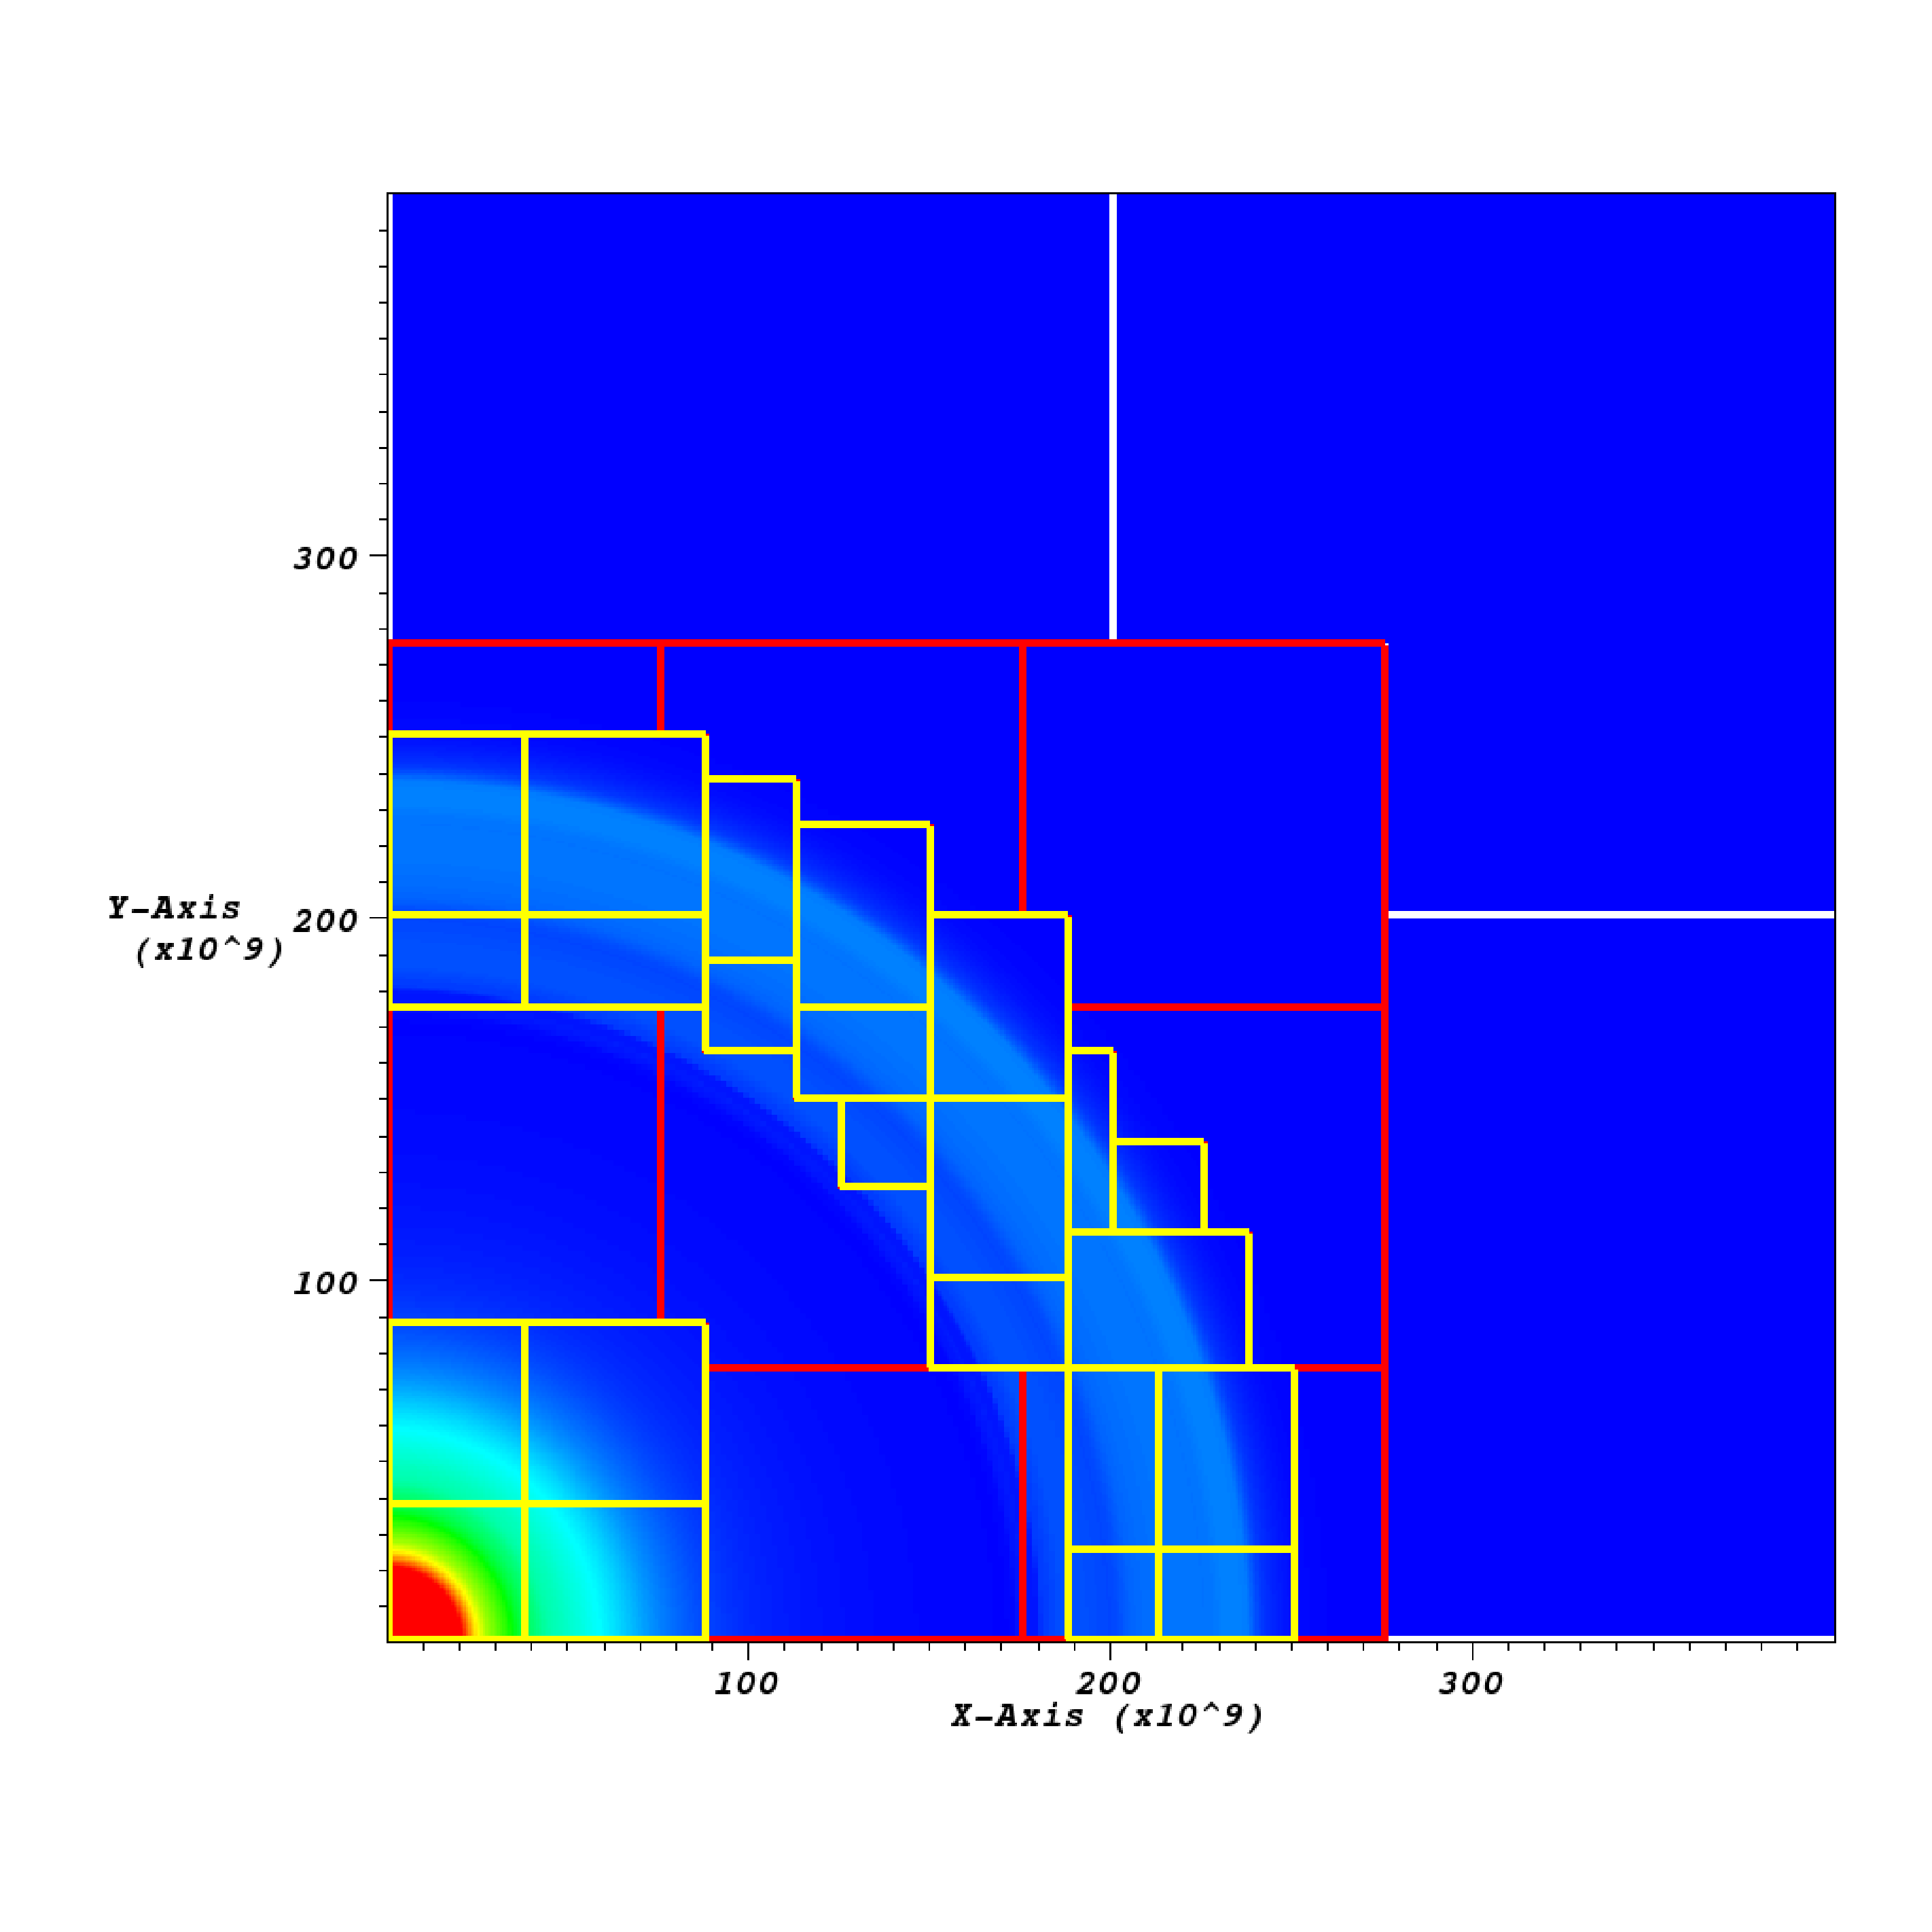
\includegraphics[width=3in]{orig_corner}
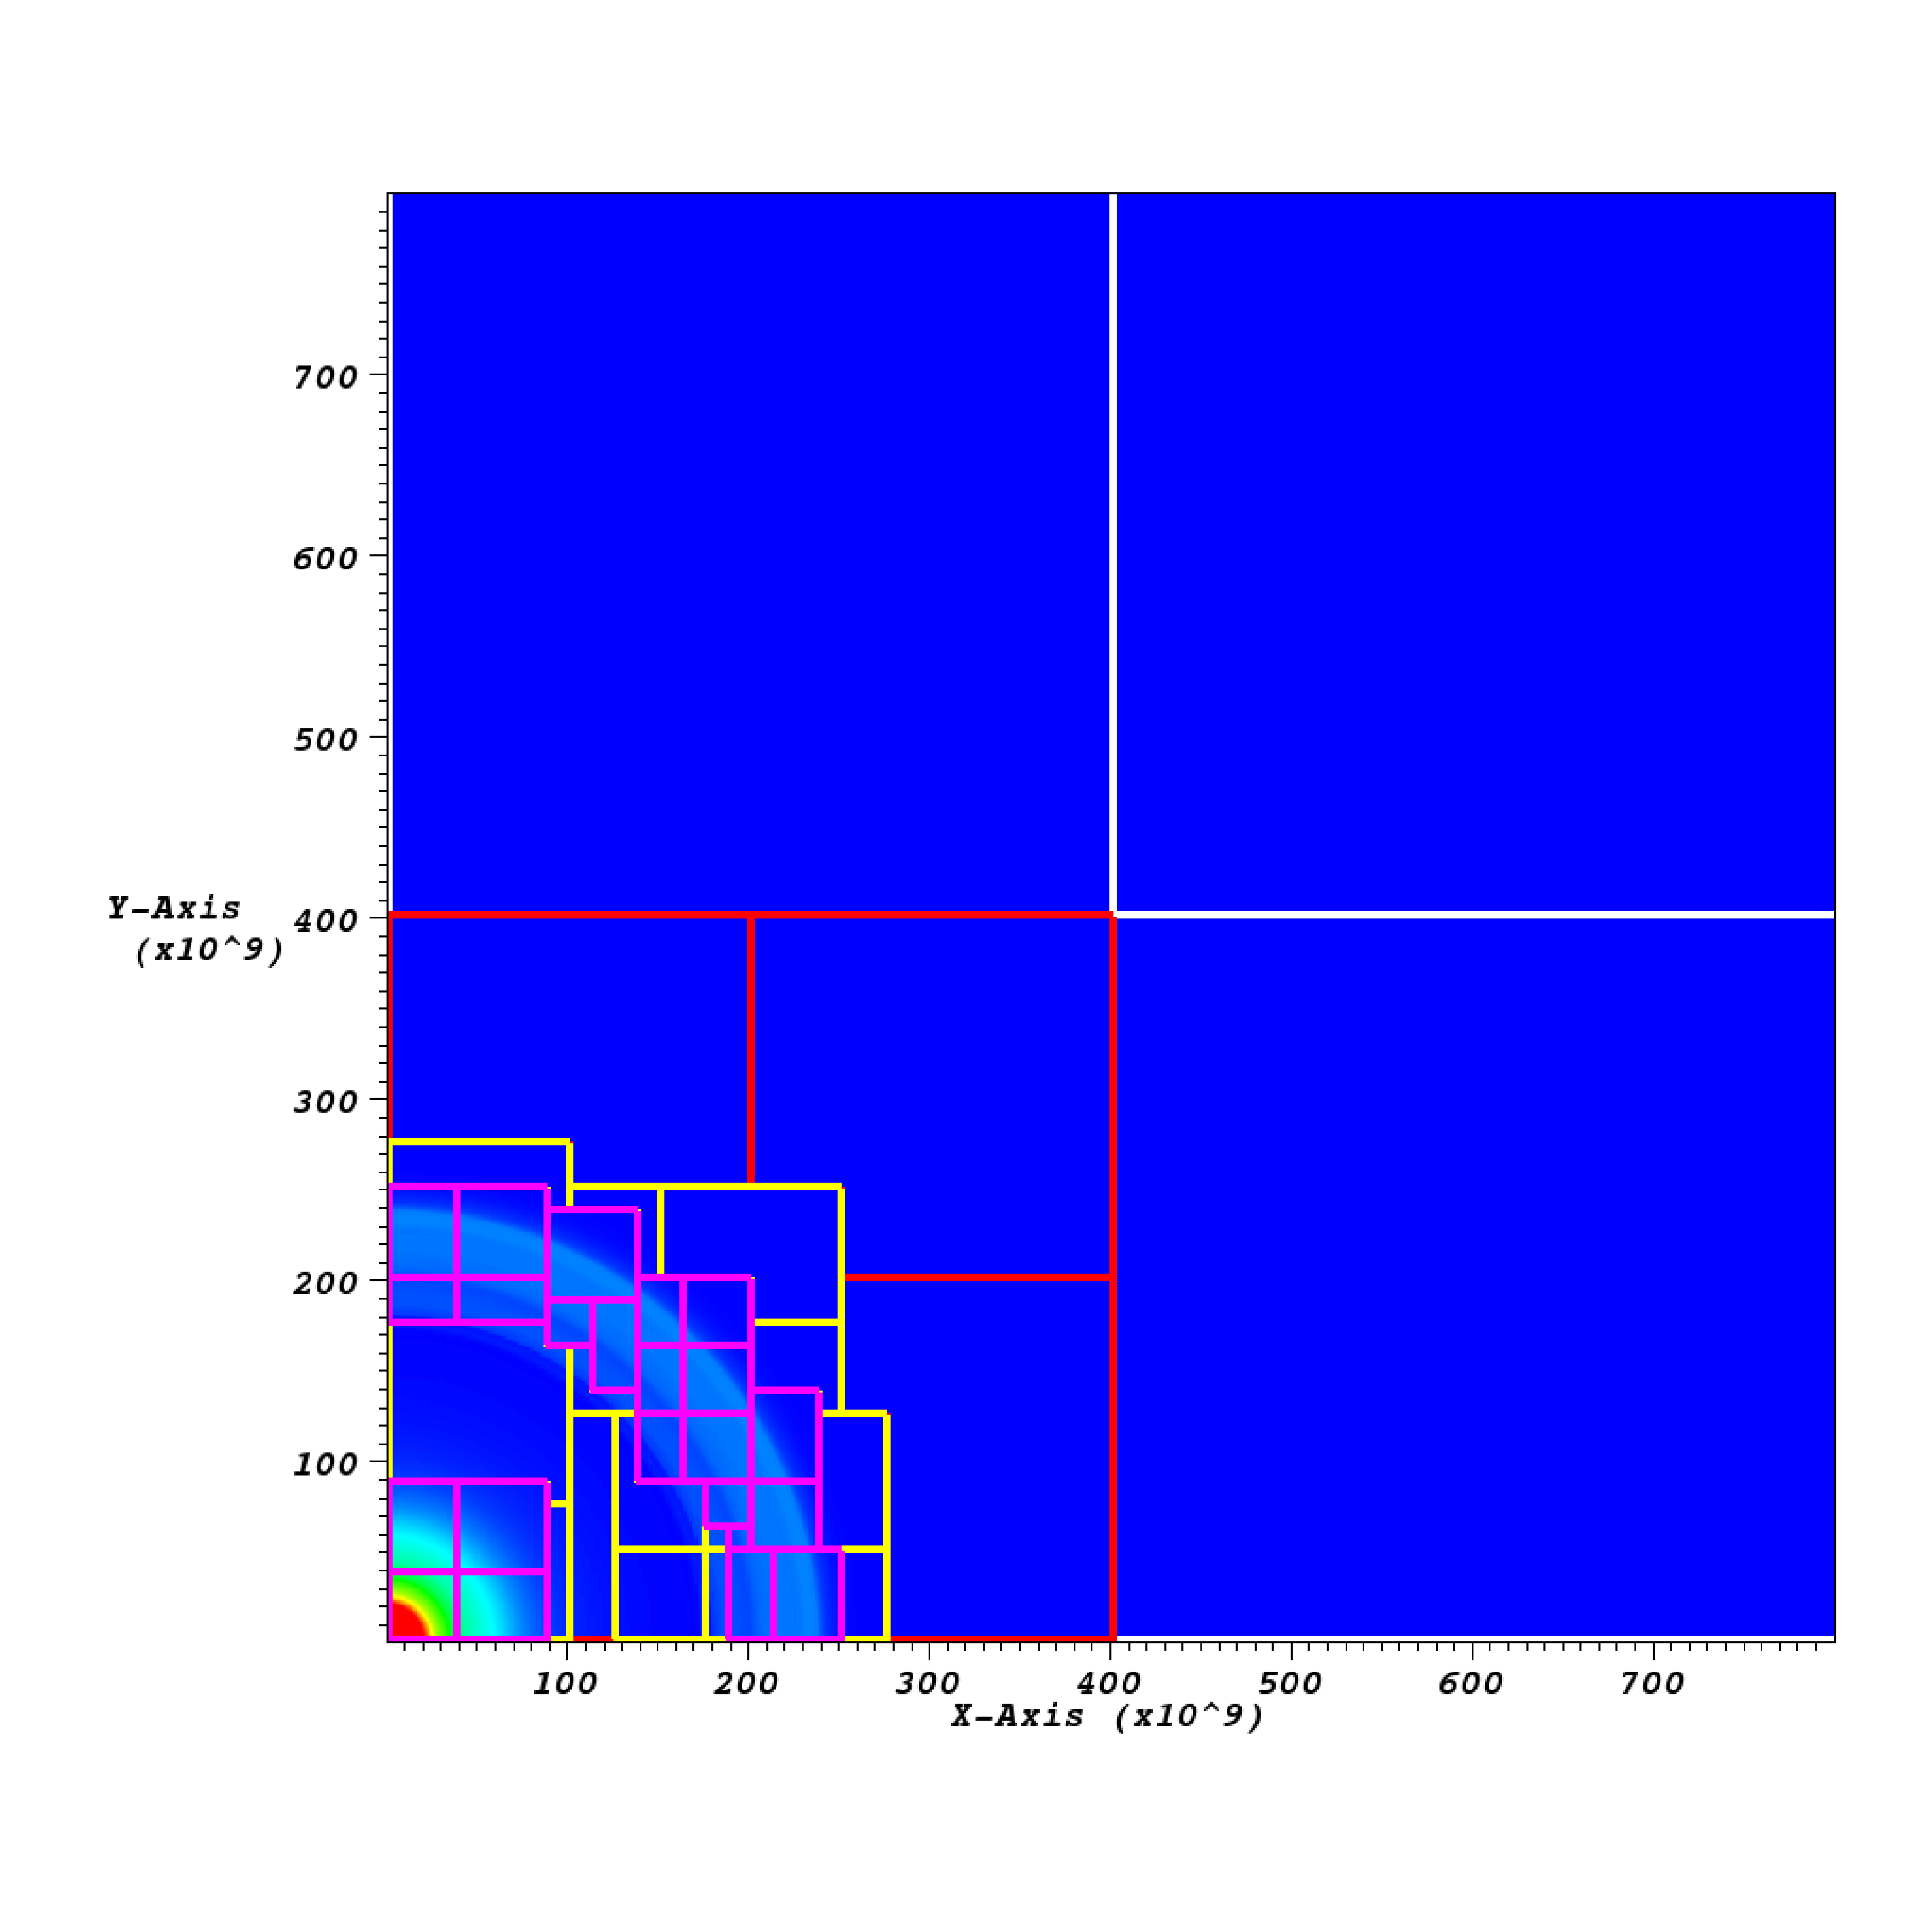
\includegraphics[width=3in]{grown_corner_2}
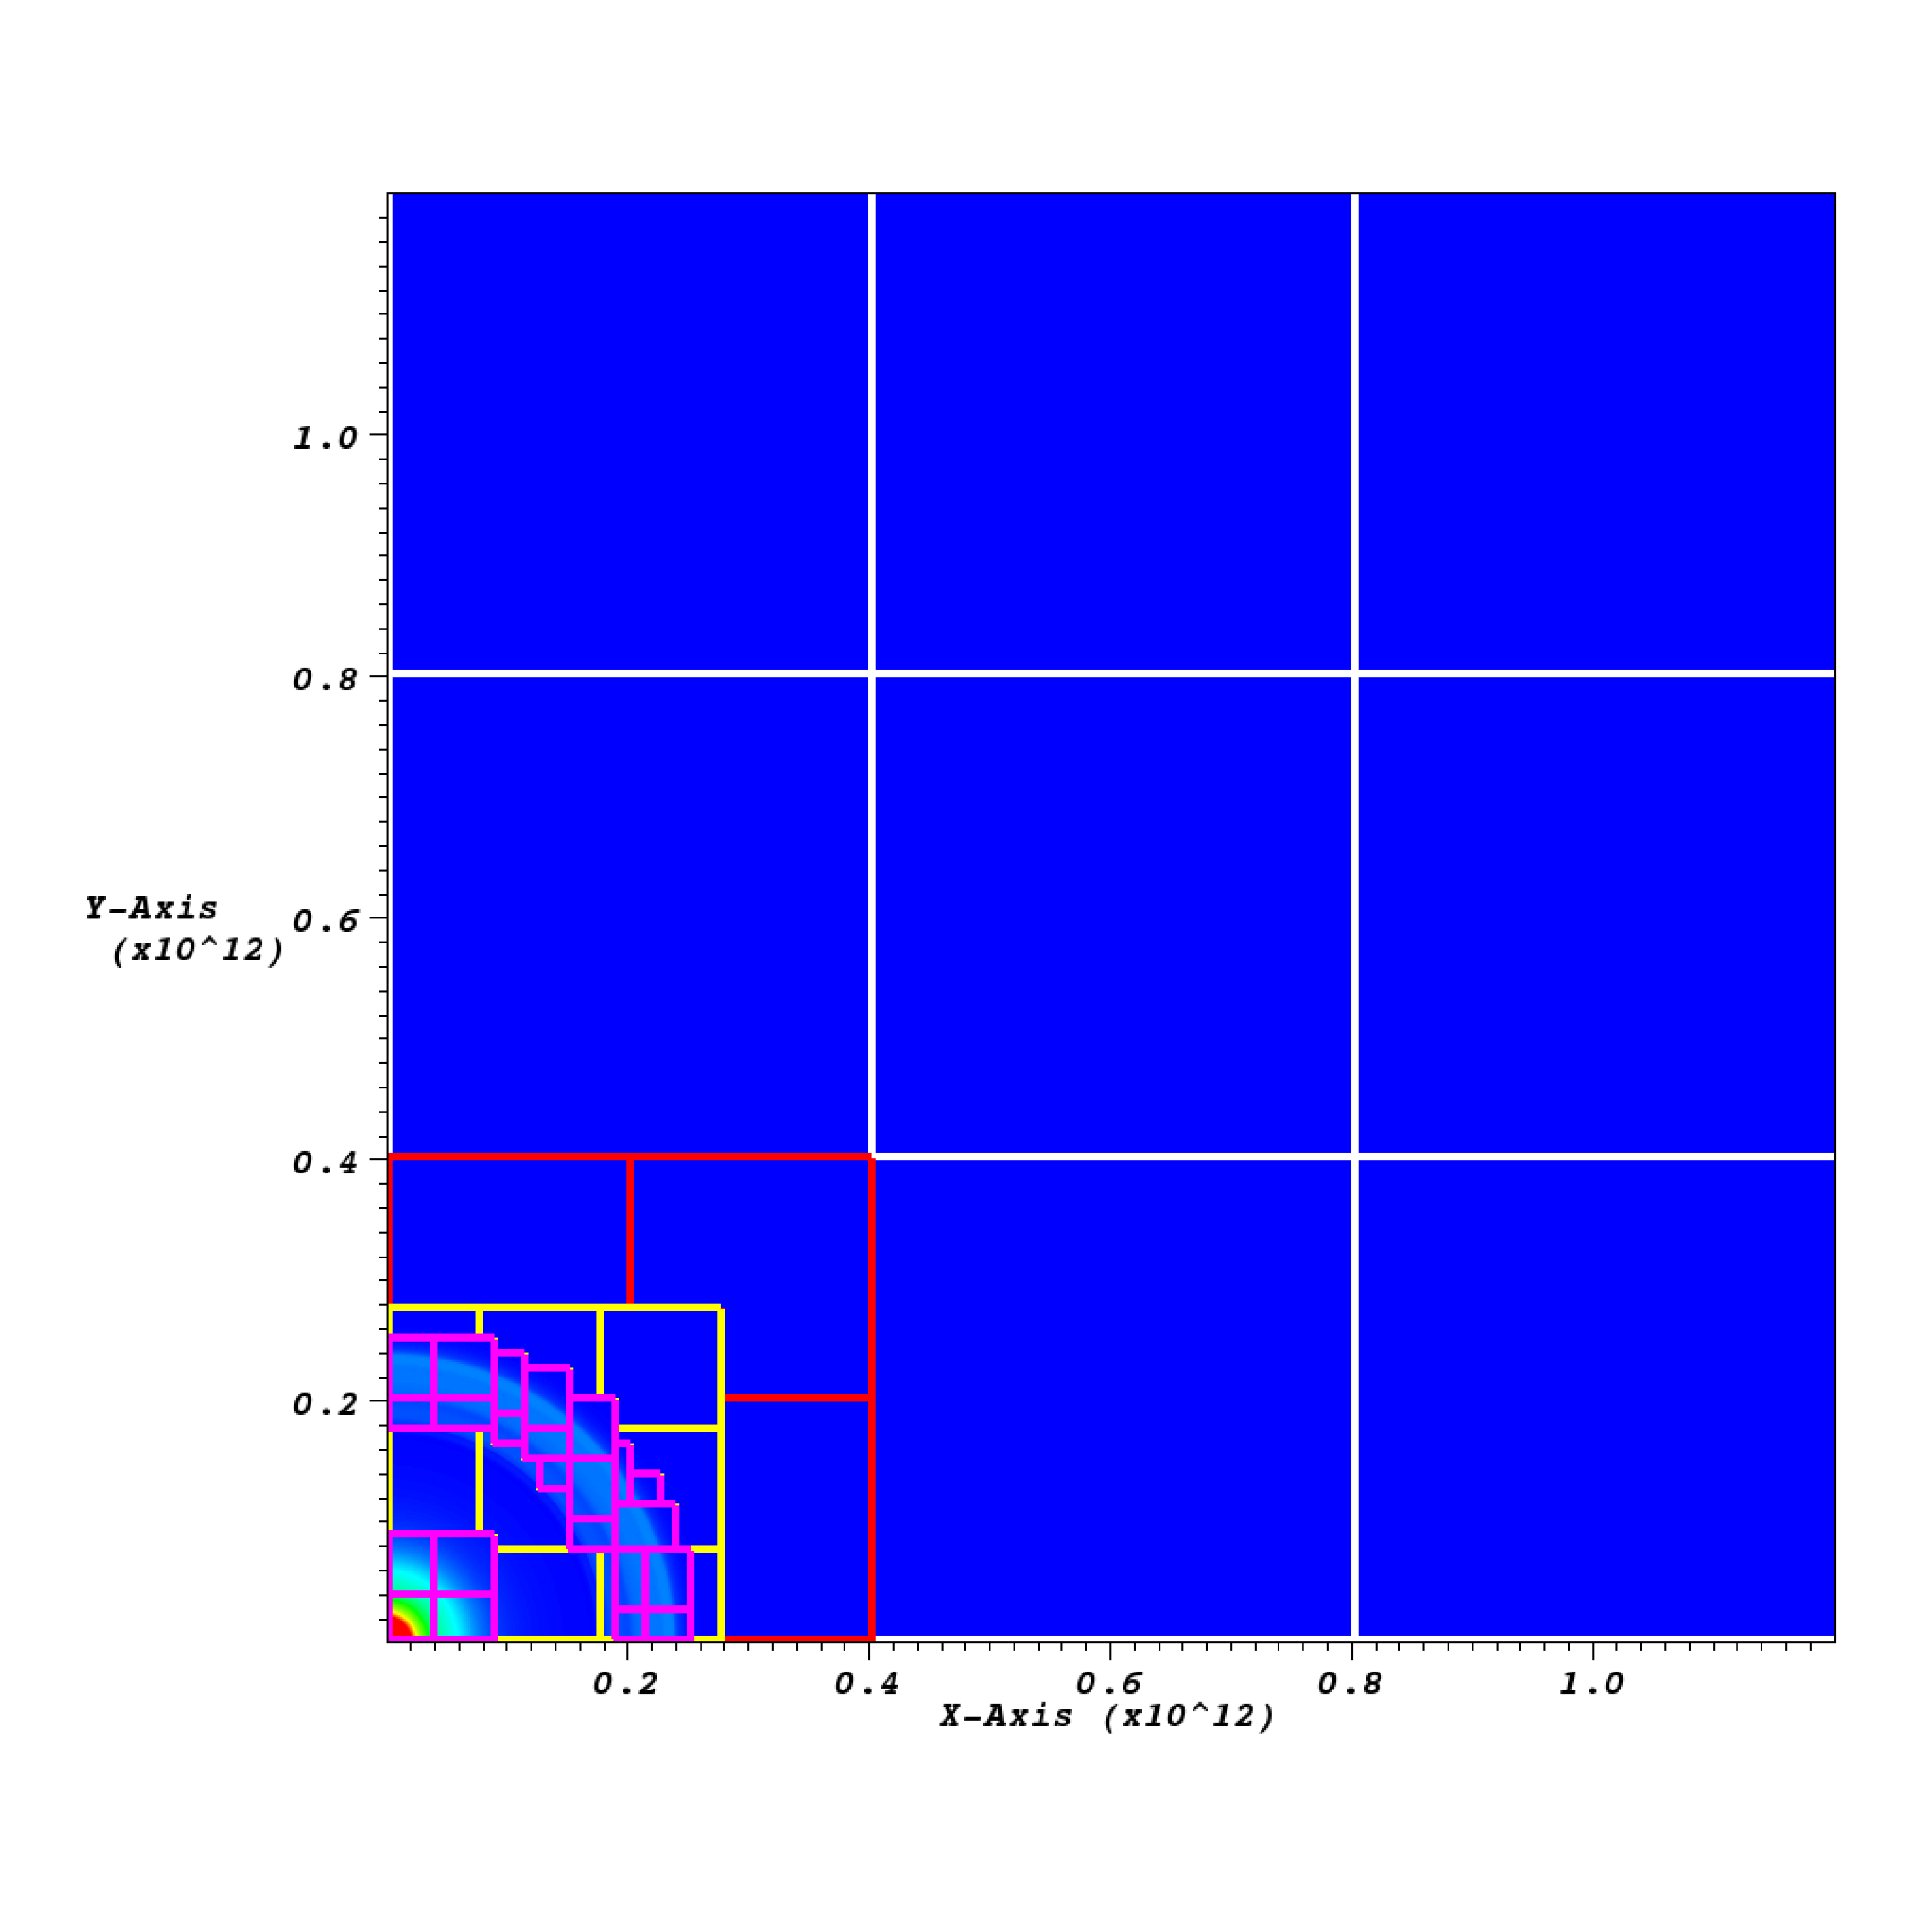
\includegraphics[width=3in]{grown_corner_3}
\caption{Data from checkpoint file before and after the domain has been coarsened and grown.  This case
uses {\bf star\_at\_center = 0}  and {\bf ref\_ratio}=2.  The first grown example has 
{\bf grown\_factor}=2,  the second has {\bf grown\_factor}=3.  In all figures the level 0 grids 
are shown in white, the level 1 grids in red, the level 2 grids in yellow, and in the grown figures, 
the level 3 grids are in pink.}
\end{figure}
%%%%%%%%%%%%%%%%%%%%%%%%%%%%%%%%%

%%%%%%%%%%%%%%%%%%%%%%%%%%%%%%%%%
\begin{figure}[h]
\centering
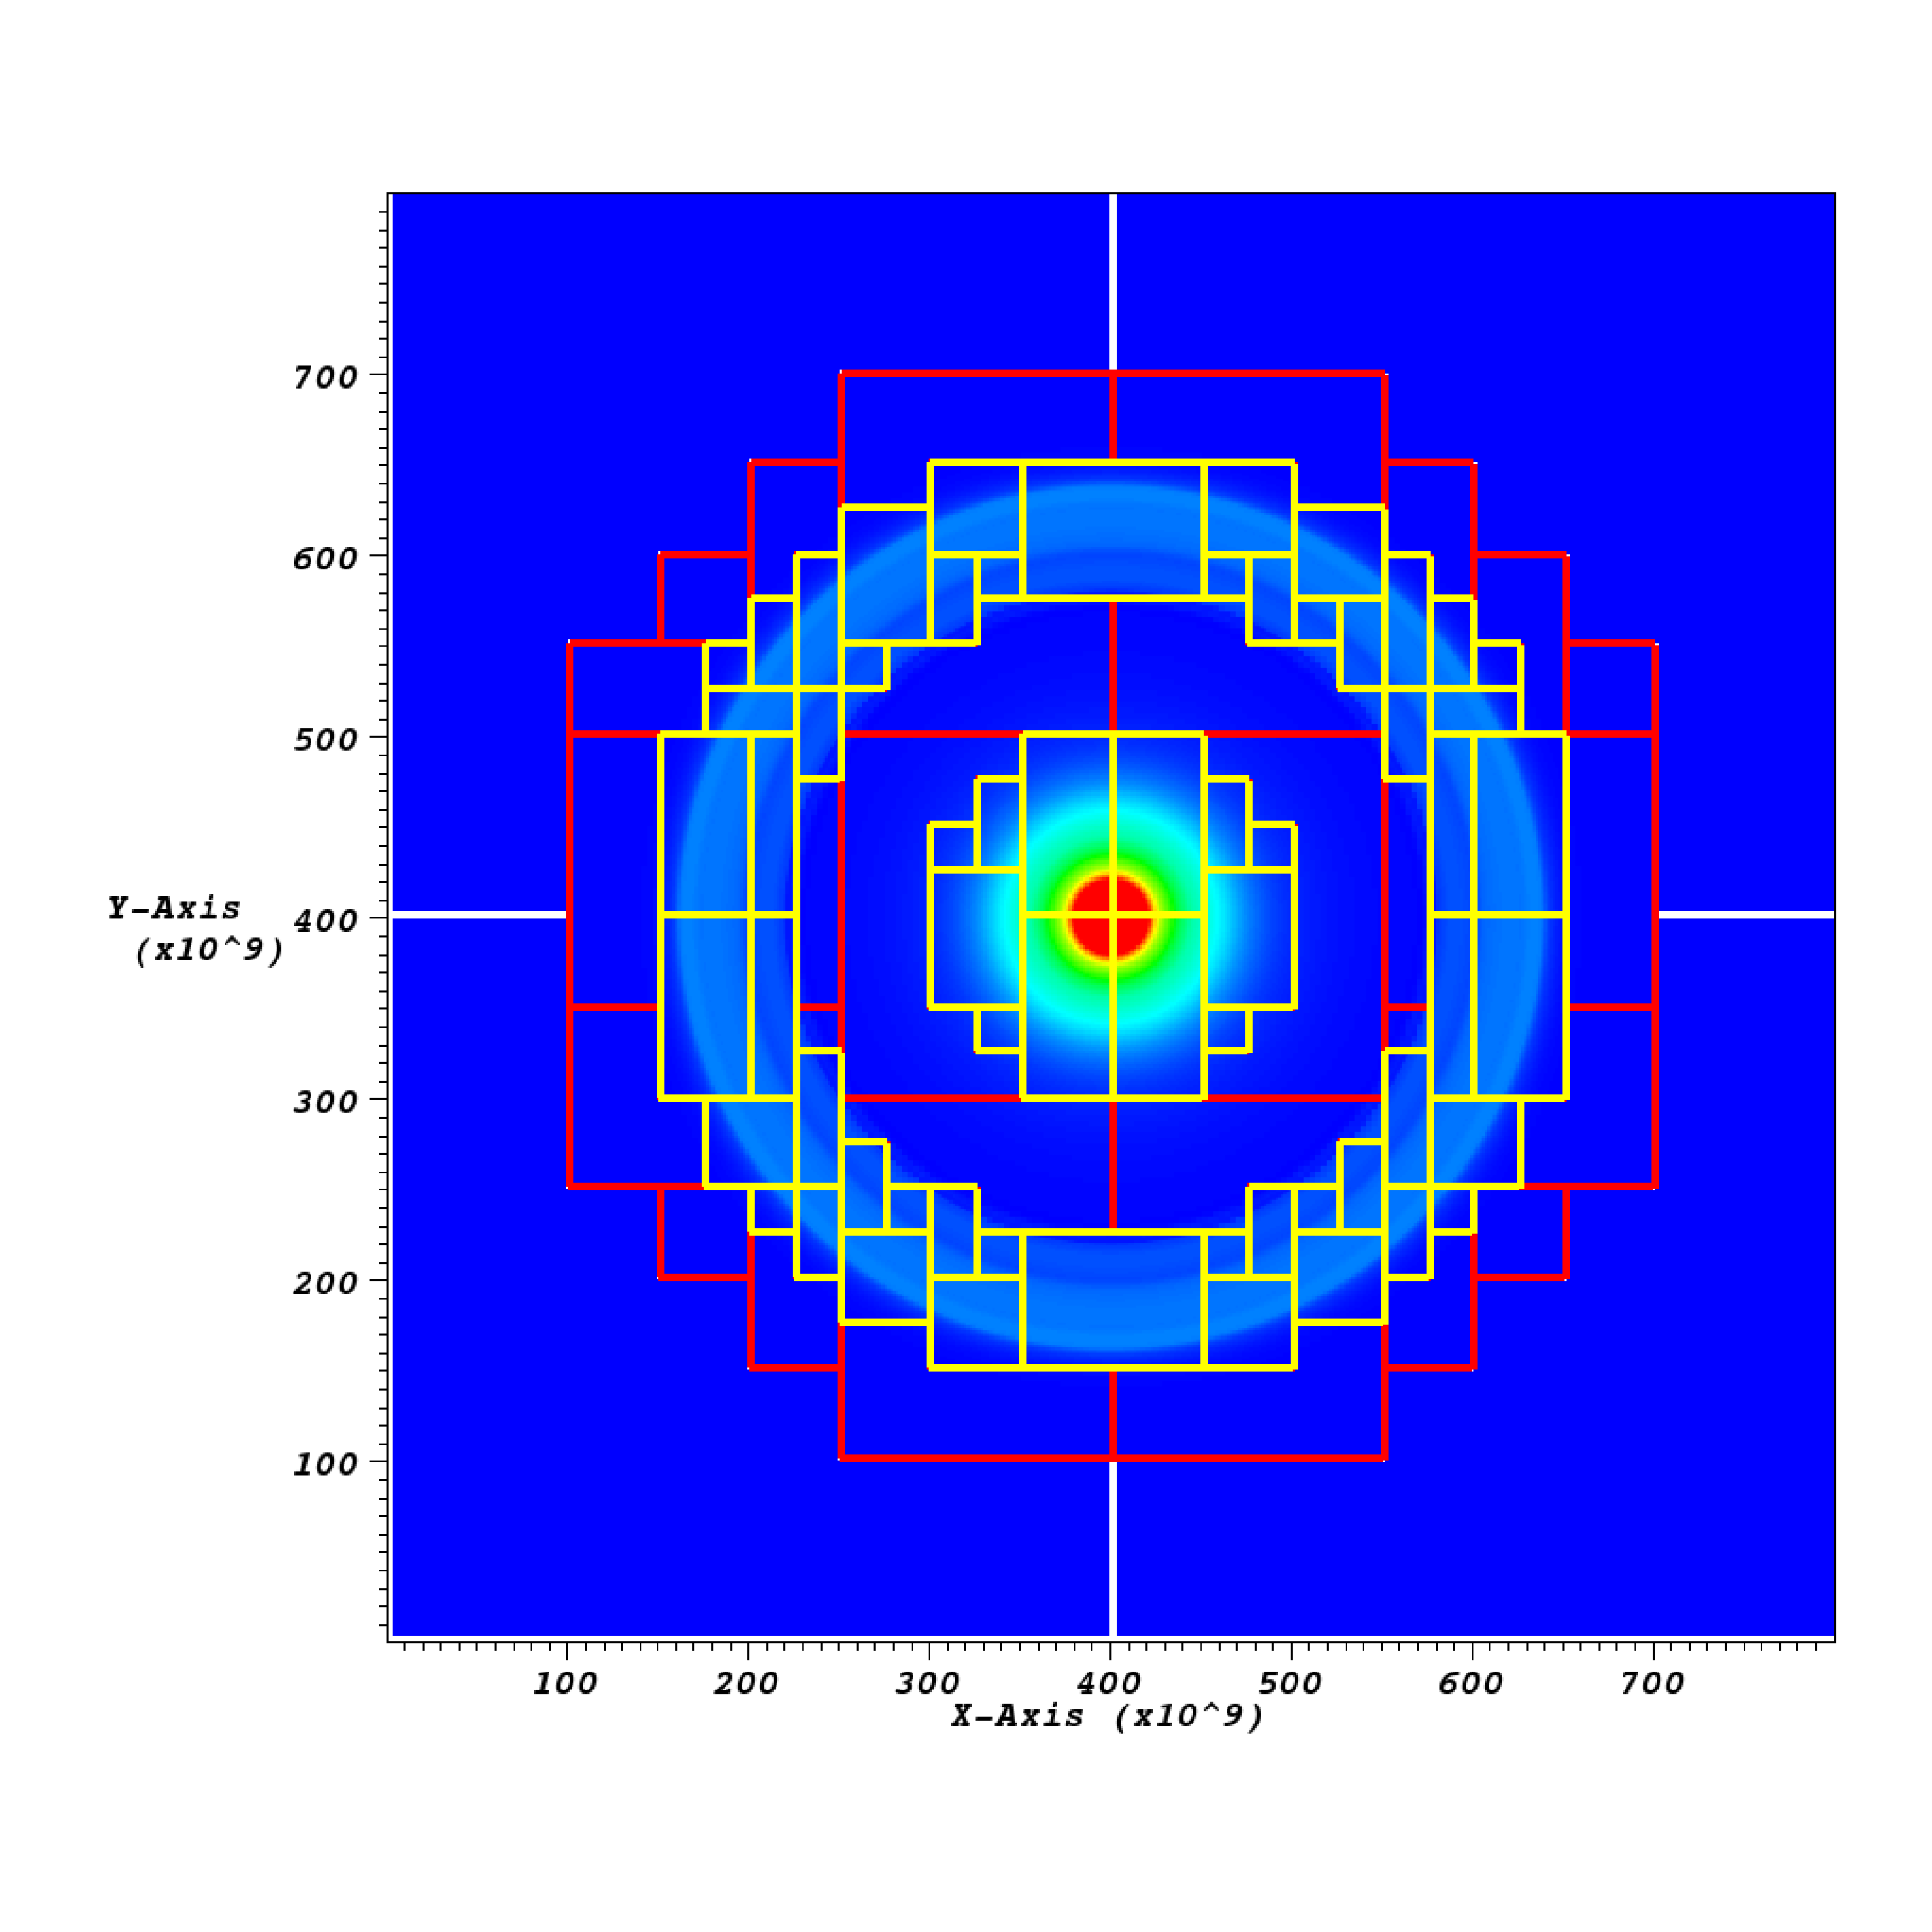
\includegraphics[width=3in]{orig_center}
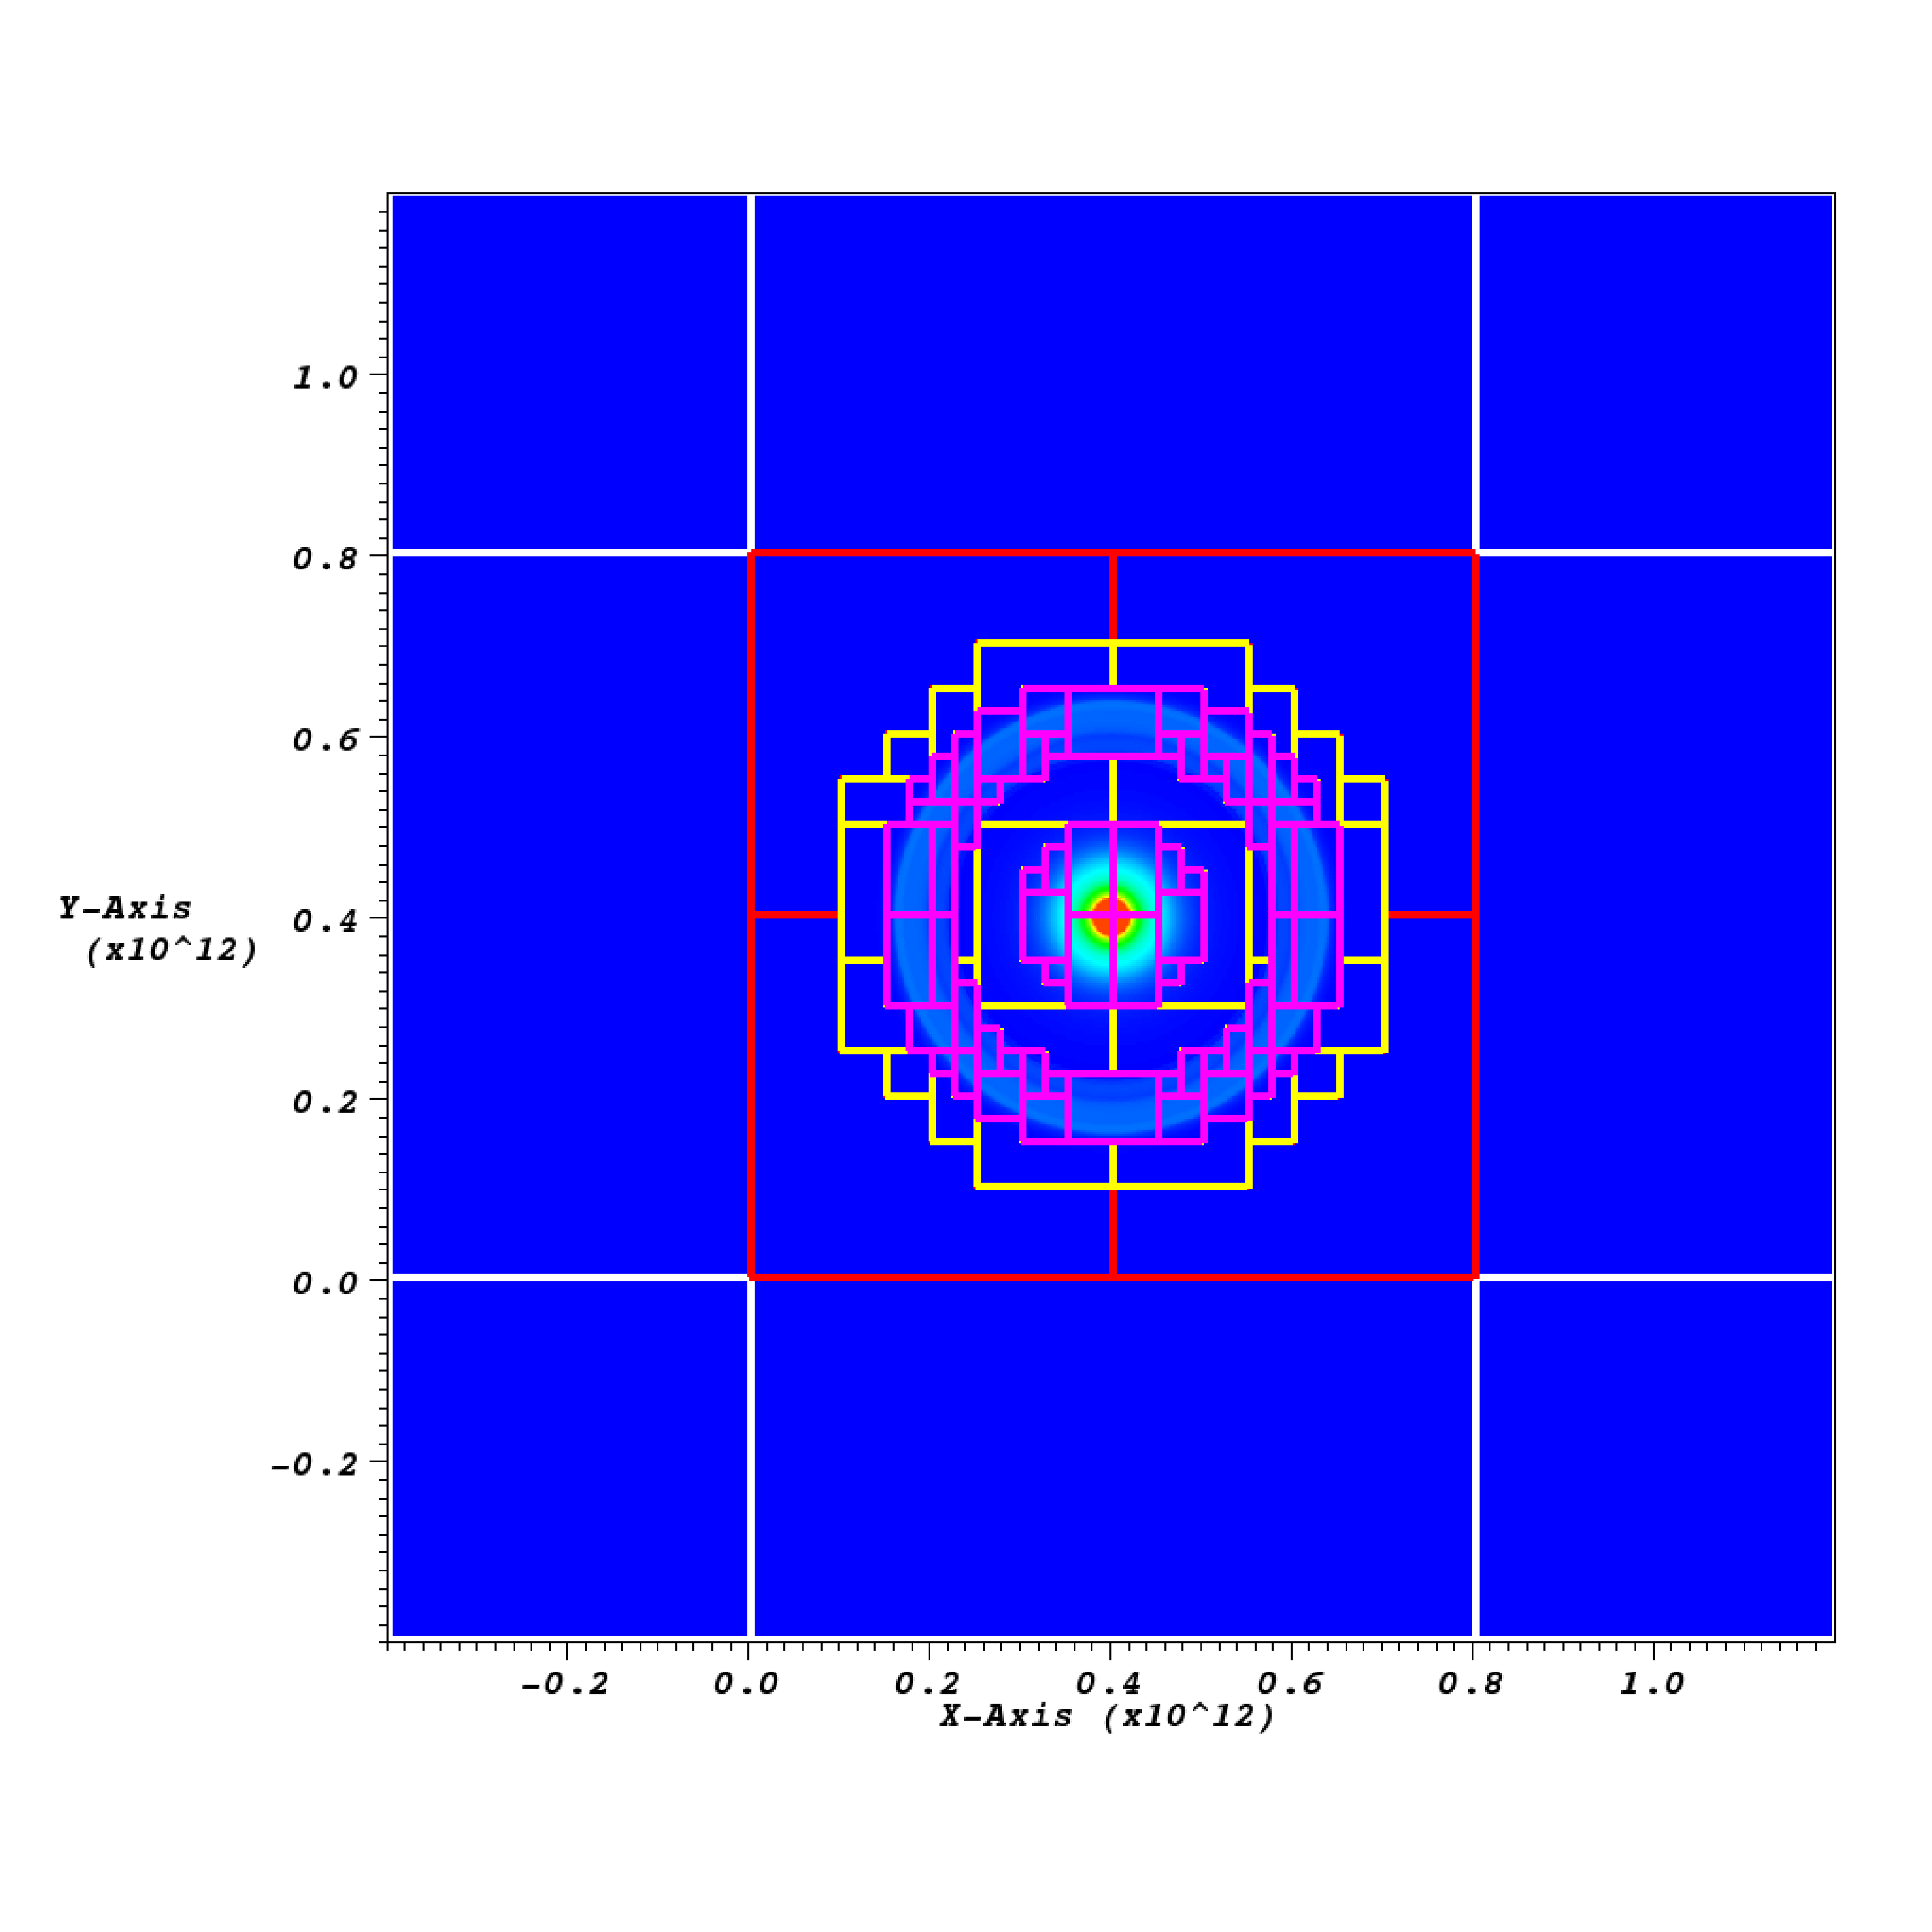
\includegraphics[width=3in]{grown_center_2}
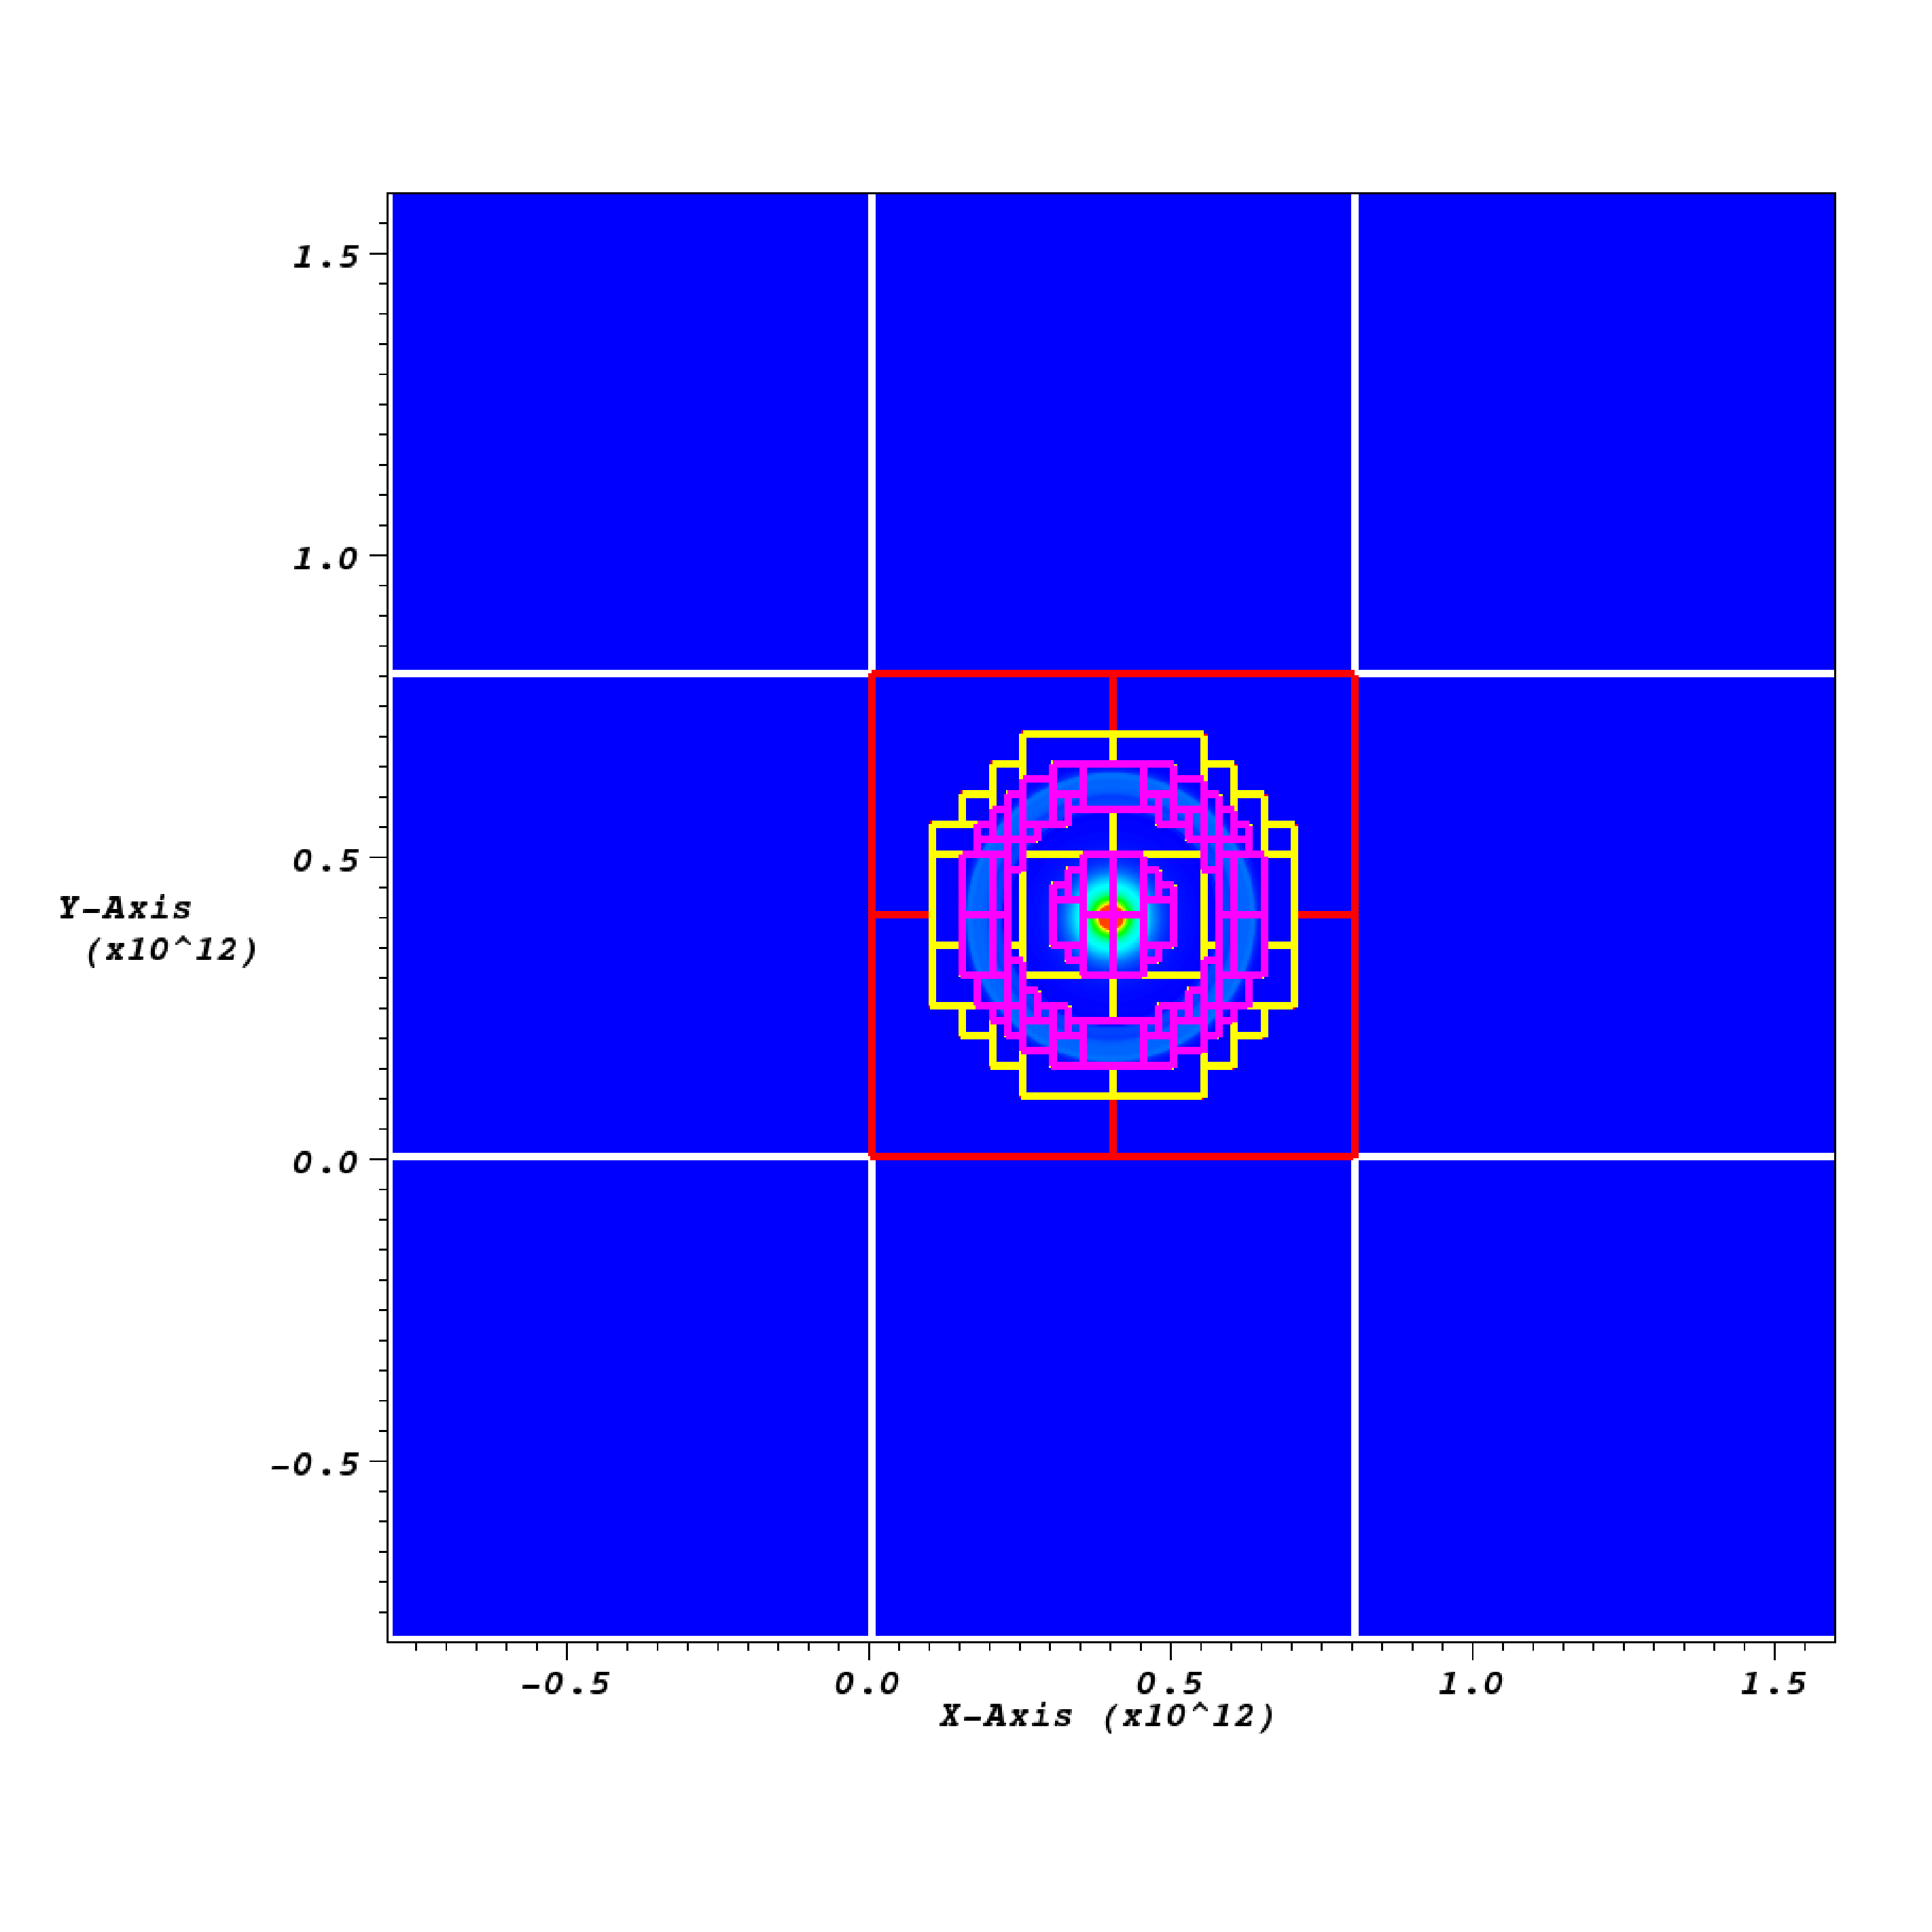
\includegraphics[width=3in]{grown_center_3}
\caption{Data from checkpoint file before and after the domain has been coarsened and grown.  This case
uses {\bf star\_at\_center = 0}  and {\bf ref\_ratio}=2.  The first grown example has 
{\bf grown\_factor}=2,  the second has {\bf grown\_factor}=3.  In all figures the level 0 grids 
are shown in white, the level 1 grids in red, the level 2 grids in yellow, and in the grown figure, 
the level 3 grids are in pink. }
\end{figure}
%%%%%%%%%%%%%%%%%%%%%%%%%%%%%%%%%



\chapter{Initializing \castro\ with \maestro\ Data}
\section{Overview}
We can now initialize a \castro\ simulation using data from a \maestro\
plotfile.  This should not be thought of as a restart mode, but rather
a new simulation with a special initialization.  In order to use this
feature, you must make sure the \maestro\ plotfile has the proper
variables, add some new parameters to your inputs file, and add a few
subroutines to Prob\_Xd.f90.  You need to build a special executable
with ``USE\_MAESTRO\_INIT=TRUE'', which will add ``.MAESTRO'' to the
executable string.  For multilevel problems, there are a few extra
steps relating to the fact that you have to supply a grids file
consistent with the \maestro\ grid structure.

\section{MAESTRO Plotfile Requirements}
The \maestro\ plotfile needs to have the following variables:
\begin{itemize}
\item ``x\_vel'', ``y\_vel'', (and ``z\_vel'', depending on
  dimensionality of the problem)
\item ``density'' ({\bf castro.MAESTRO\_init\_type} = 1 and 2 only)
\item Optional species (such as ``X(C12)'') - there is an option to
  not read any species from the \maestro\ plotfile.  In this case, you
  must make sure your code manually defines the species cell-by-cell
  in the initial \castro\ data
\item ``tfromp''
\item ``pi'' ({\bf castro.MAESTRO\_init\_type} = 2, 3, and 4 only)
\item ``entropy'' ({\bf castro.MAESTRO\_init\_type} = 4 only)
\end{itemize}
Also, model\_cc\_XXXXX needs to list variables in the following order,
which is the default order found in {\tt MAESTRO/Source/base\_io.f90}: r,
base\_r, rho0, p0, gamma1bar, rhoh0, div\_coeff, psi, tempbar,
etarho\_cc, tempbar\_init.

\section{List of Parameters}
Here are the additional parameters you must add to your inputs file.
\begin{table*}[h]
\begin{tiny}
\begin{tabular}{|l|l|l|l|} \hline
Parameter & Definition & Type & Default \\
\hline
    {\bf castro.MAESTRO\_plotfile} & name of the \maestro\ plotfile & std::string & must be set \\
    
    {\bf castro.MAESTRO\_modelfile} & name of the \maestro\ ``model\_cc'' file & std::string & must be set \\
    
    {\bf castro.MAESTRO\_npts\_model} & number of points in the \maestro\ model\_cc file & int & must be set \\
    
    {\bf castro.MAESTRO\_first\_species} & name of the first species & std::string & must be set or else nothing will be read in \\
    
    {\bf castro.MAESTRO\_nspec} & number of species in the \maestro\ plotfile & std::string & NumSpec in \castro \\
    
    {\bf castro.MAESTRO\_cutoff\_density} & controls how we overwrite data at the edge of the star & Real & must be set \\
    
    {\bf castro.MAESTRO\_init\_type} & determines how we initialize the \castro\ state & int & must be set \\
    
    {\bf castro.MAESTRO\_spherical} & specifies planar or spherical problem & int & must be set \\
    
\hline
\end{tabular}
\end{tiny}
\end{table*}

\subsection{Examples of Usage}
\begin{itemize}
\item {\bf castro.MAESTRO\_plotfile} = "wd\_384\_6.25e8K\_norotate\_plt120578"
\item {\bf castro.MAESTRO\_modelfile} = "./wd\_384\_6.25e8K\_norotate\_plt120578/model\_cc\_120578"
\item {\bf castro.MAESTRO\_npts\_model} = 1663\\ This is the number of
  points in {\bf castro.MAESTRO\_modelfile}.  Note that this is not
  the same thing as ``npts\_model'', which is the number of points in
  the initial model file used for standard simulations where we do not
  initialize from a \maestro\ plotfile.
\item {\bf castro.MAESTRO\_first\_species} = ``X(C12)'' If you do not
  specify this, no species will be read in.  You can always manually
  specify or overwrite the species cell-by-cell later.
\item {\bf castro.MAESTRO\_nspec} = 3\\ If you do not specify this, it
  will default to the number of species in the \castro\ network,
  ``NumSpec''.  We have this here because sometimes \maestro\ and \castro\
  will use different networks with different number of species.
\item {\bf castro.MAESTRO\_cutoff\_density} = 1.e6\\ The code will use
  this density to figure out the radial coordinate, r\_model\_start,
  which is the last radial coordinate before rho0 falls below {\bf
    castro.MAESTRO\_cutoff\_density}.  It is possible to set {\bf
    castro.MAESTRO\_cutoff\_density} to a tiny value, such that rho0
  never falls below this value, in which case we set r\_model\_start
  to $\infty$.  In INITDATA\_MAKEMODEL, we create a new 1D model
  integrating outward starting from r\_model\_start.  Then, in
  INITDATA\_OVERWRITE, we overwrite newly initialized \castro\ data in
  any cell that maps into a radial coordinate greater than
  r\_model\_start by interpolating from the new 1D model.
\item {\bf castro.MAESTRO\_init\_type} = 2\\ \castro\ will read in data
  from the \maestro\ plotfile, and then call the EOS to make sure that
  $\rho$, $e$, $T$, and $X_k$ are consistent.  The inputs to the EOS
  are based on the value of {\bf castro.MAESTRO\_init\_type}:
\begin{enumerate}
\item $e = e(\rho,T,X_k)$
\item $e,T = e,T(\rho,p_0+\pi,X_k)$
\item $\rho,e = \rho,e(p_0+\pi,T,X_k)$
\item $\rho,T,e = \rho,T,e(p_0+\pi,s,X_k)$
\end{enumerate}
\item {\bf castro.MAESTRO\_spherical} = 1\\
0 = planar; 1 = spherical.
\end{itemize}

\section{New Subroutines in Prob\_Xd.f90}
There are three routines that need to be added to your local copy of
{\tt Prob\_Xd.f90}.  See {\tt Castro/Exec/wdconvect/Prob\_3d.f90} for
a standard spherical \maestro\ initialization.
\begin{enumerate}
\item INITDATA\_MAESTRO\\ This fills in the \castro\ state by taking
  the \maestro\ data, calling the EOS, and making the proper variables
  conserved quantities.  Specifically, we need a thermodynamically
  consistent $\rho$, $T$, $e$, and $X_k$, and then algebraically
  compute $\rho{\bf u}$, $\rho e$, $\rho E$, and $\rho X_k$,
\item INITDATA\_MAKEMODEL\\
This creates a user-defined 1D initial model starting from r\_model\_start.
\item INITDATA\_OVERWRITE\\ This overwrites the initialized \castro\
  data using the new 1D initial model for all cells that map into
  radial coordinates greater than r\_model\_start.
\end{enumerate}

\section{Additional Notes}
Note that for both single-level and multilevel \maestro\ to \castro\
initialization, the \castro\ base grid structure does not have to match
the \maestro\ base grid structure, as long as the problem domain is the
same.  For example, if the coarsest level in a \maestro\ plotfile
contains $64^3$ cells divided into 8-$32^3$ grids, it is ok to use a
\castro\ base grid structure with 1-$64^3$ grid, 64-$16^3$ grids, or
anything else you can imagine - the grids don't even have to be the
same size.  As is normally the case, the \castro\ base grid structure is
created based on the parameters in the \castro\ inputs file, such as
{\bf amr.max\_grid\_size}, {\bf amr.blocking\_factor}, etc.

\subsection{Multilevel Restart}
When initialing from a multilevel \maestro\ plotfile, there are some
extra steps.  First, you need to create a \castro-compatible grids file
from the \maestro\ plotfile.  This can be done with the {\tt
  BoxLib/Tools/Postprocessing/F\_Src/fboxinfo.f90} utility.  Compile
and run this using the ``\texttt{--}castro'' option, e.g.,
``fboxinfo.Linux.gfortran.exe \texttt{--}castro pltxxxxx \texttt{|}
tee gr0.maestro'', to generate the \castro-compatible grids file.  Note
that the base grid structure is still controlled by {\bf
  amr.max\_grid\_size}, {\bf amr.blocking\_factor}, etc., since in C++
BoxLib, the grids file only indicates the refined grid structure,
whereas in Fortran BoxLib the grids file contains the base grid and
refined grid structures.

Now, when you initialize the \castro\ simulation, you need to specify
the grid file using {\bf amr.regrid\_file = "gr0\_3d.128\_2levels"},
for example.  You can happily run this now, but note that the
regridding algorithm will never be called (since \castro\ thinks it's
started a new simulation from scratch with a grids file, thus
disabling the regridding).  If you wish for the grid structure to be
changed, you must do a traditional \castro\ restart from the
\castro-generated checkpoint file (you can still use the same
``.MAESTRO'' executable or an executable built with
USE\_MAESTRO\_INIT=FALSE), making sure that you {\bf do not} specity
{\bf amr.regrid\_file} (or else the grids will stay fixed).  You are
free to specify {\bf amr.regrid\_on\_restart}, {\bf
  amr.compute\_new\_dt\_on\_regrid}, and {\bf
  amr.plotfile\_on\_restart}.

Sometimes a \maestro\ plotfile will only have 1 or 2 total levels, but
you ultimately want to run a \castro\ simulation with many more levels
of refinement.  My recommended strategy is the following:
\begin{enumerate}
\item Initialize a \castro\ simulation from the \maestro\ plotfile
  while preserving the exact same grid structure and run for 10 time
  steps.
\item Do a traditional \castro\ restart from {\tt chk00010}, but do not
  increase {\bf amr.max\_level}, and run for 10 more time steps.  This
  allows a new grid structure with the same effective resolution as
  before settle in using the C++ BoxLib regridding algorithm.
\item Do a traditional \castro\ restart from {\tt chk00020}, but increase
  {\bf amr.max\_level} by 1, and run for 10 time steps.
\item Repeat the procedure from the previous step (using the most
  updated checkpoint of course) as many times as desired.
\end{enumerate}


\chapter{Visualization}
\section{2D and 3D}
\subsection{amrvis}
Our favorite visualization tool is amrvis. We heartily encourage you to build the amrvis2d and amrvis3d executables, and to try using them to visualize your data. A very useful feature is View/Dataset, which allows you to actually view the numbers -- this can be handy for debugging. You can modify how many levels of data you want to see, whether you want to see the grid boxes or not, what palette you use, etc.

If you like to have amrvis display a certain variable, at a certain scale, when you first bring up each plotfile (you can always change it once the amrvis window is open), you can modify the amrvis.defaults file in your directory to have amrvis default to these settings every time you run it. The directories CoreCollapse, HSE\_test, Sod and Sedov have amrvis.defaults files in them. If you are working in a new run directory, simply copy one of these and modify it.
\subsection{VisIt}
VisIt is also a great visualization tool, and it directly handles our plotfile format (which it calls Boxlib).  For more information check out visit.llnl.gov.

[Useful tip:] To use the Boxlib3D plugin, select it from File $\rightarrow$ Open file $\rightarrow$ Open file as type Boxlib, and then the key is to read the Header file, plt00000/Header, for example, rather than telling to to read plt00000.

\section{Controlling What's in the PlotFile}

{\bf amr.plot\_vars} = \\

\noindent and  \\

\noindent {\bf amr.derive\_plot\_vars} = \\

\noindent are used to control which variables are included in the plotfiles.  The default for {\bf amr.plot\_vars}
is all of the state variables.  The default for {\bf amr.derive\_plot\_vars} is none of
the derived variables.  So if you include neither of these lines then the plotfile
will contain all of the state variables and none of the derived variables. \\

\noindent If you want all of the state variables plus entropy and pressure, for example, then set \\

\noindent {\bf amr.derive\_plot\_vars} = entropy pressure \\

\noindent If you just want density and pressure, for example, then set \\

\noindent {\bf amr.plot\_vars} =  density \\

\noindent {\bf amr.derive\_plot\_vars} = pressure \\

\section{1D}
amrvis doesn't like 1-d plotfiles, and for those we use a 1-d plotting capability installed by Mike Singer 
Castro/Util/plot1d.  If you want to make xmgrace-compatible files, for example, add the following to your inputs file:\\

{\bf xgraph.xmgrace\_file} = 1

{\bf xgraph.format} = xmg

{\bf xgraph.use\_xmgrace\_legend} = 1

{\bf xgraph.use\_xmgrace\_title} = 1

{\bf xgraph.graph} = xvel x\_velocity 100 -1\\ \\
This tells is to write a file called xvel\_0000.xmgr, for example, every 100 time steps, including all levels of data. (The last variable, -1, specifies the maximum level; if it is -1 then all levels are used.)

If you want to write more than one variable into a single file, then instead of
setting each variable on a separate line as in the xvel example above,
you can do the following: \\

\noindent {\bf xgraph.graph} = file\_name ALL 100 -1\\

\noindent If you specify ``ALL'' then \\

\noindent {\bf amr.plot\_vars} = \\

\noindent and \\

\noindent {\bf amr.derive\_plot\_vars} = \\

\noindent are used to control which variables are included.  The default for {\bf amr.plot\_vars}
is all of the state variables.  The default for {\bf amr.derive\_plot\_vars} is none of
the derived variables.  So if you include neither of these lines then the file 
file\_name.xmg will contain all of the state variables and none of the derived variables.

If you want all of the state variables plus entropy and pressure, for example, then set \\

{\bf amr.derive\_plot\_vars} = entropy pressure \\

{\bf xgraph.graph} = file\_name ALL 100 -1\\

If you just want density and pressure, for example, then set \\

{\bf amr.plot\_vars} =  density \\

{\bf amr.derive\_plot\_vars} = pressure \\

{\bf xgraph.graph} = file\_name ALL 100 -1\\ 

Feel free to read the routines in Castro/Util/plot1d.


\chapter{Verification Test Problems}

%%%%%%%%%%%%%%%%%%%%%%%%%%%%%%%%%%%%%%%%%%%%%%%%%%%%%%%%%%%%%%%%%%%%%%%%%%%%%%%
\section{Hydrodynamics Test Problems}

\subsection{Sod's Problem (and Other Shock Tube Problems)}

The {\tt Exec/Sod} problem directory sets up a general one-dimensional
shock tube.  The left and right primitive-variable states are specified
and the solution evolves until a user-specified end time.  For a simple
discontinuity, the exact solution can be found from an exact Riemann 
solver.  For this problem, the exact solutions were computed with the
exact Riemann solver from Toro \cite{toro:1997}, Chapter 4.

\subsubsection{Sod's Problem}

The Sod problem \cite{sod:1978} is a simple shock tube problem that
exhibits a shock, contact discontinuity, and a rarefaction wave.
The initial conditions are:
\begin{equation}
\begin{array}{l}
\rho_L = 1 \\
u_L = 0 \\
p_L = 1
\end{array}
\qquad
\begin{array}{l}
\rho_R = 0.125 \\
u_R = 0 \\
p_R = 0.1
\end{array}
\end{equation}
The {\tt gamma\_law} equation of state is used with $\gamma = 1.4$.
The system is evolved until $t = 0.2$~s.  Setups for 1-, 2-, and 3-d
are provided.  The following inputs files and probin files setup the
Sod's problem:
\begin{table*}[h]
\centering
\begin{tabular}{|l|l|l|} \hline
\multicolumn{1}{|c}{\em inputs file} &  \multicolumn{1}{|c}{\em probin file} & \multicolumn{1}{|c|}{\em description} \\
\hline
{\tt inputs-sod-x} & {\tt probin-sod-x} & Sod's problem along $x$-direction \\
{\tt inputs-sod-y} & {\tt probin-sod-y} & Sod's problem along $y$-direction \\
{\tt inputs-sod-z} & {\tt probin-sod-z} & Sod's problem along $z$-direction \\
\hline
\end{tabular}
\label{Table:Sod}
\end{table*}

For multi-dimensional runs, the directions transverse to the jump are
kept constant.  We use a CFL number of 0.9, an initial timestep shrink
({\tt castro.init\_shrink}) of 0.1, and the maximum factor by which
the timestep can increase ({\tt castro.change\_max}) of 1.05.
\begin{figure}[h]
\centering
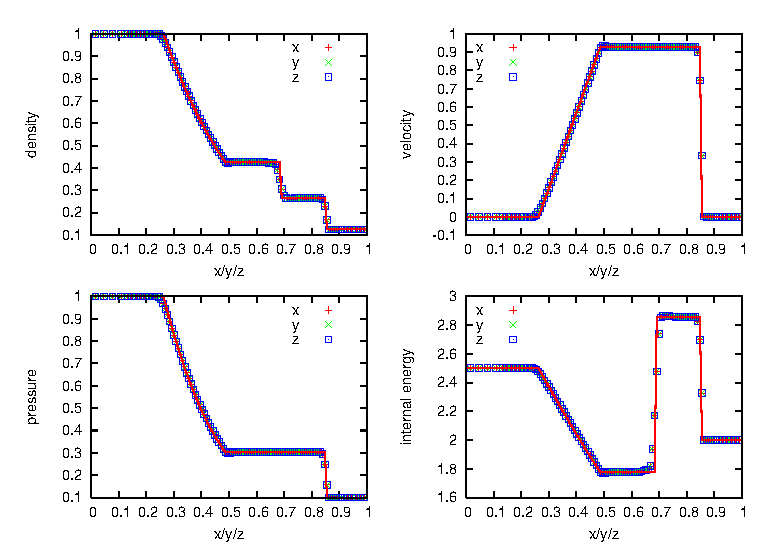
\includegraphics[width=4.75in]{CastroVerification/sod_3d}
\caption{\label{fig:sod} Castro solution for Sod's problem run in 3-d,
  with the newest ppm limiters, 
  along the $x$, $y$, and $z$ axes.  A coarse grid of 32 zones in the
  direction of propagation, with 2 levels of refinement was used.  The
  analytic solution appears as the red line.}
\end{figure}
\begin{figure}[h]
\centering
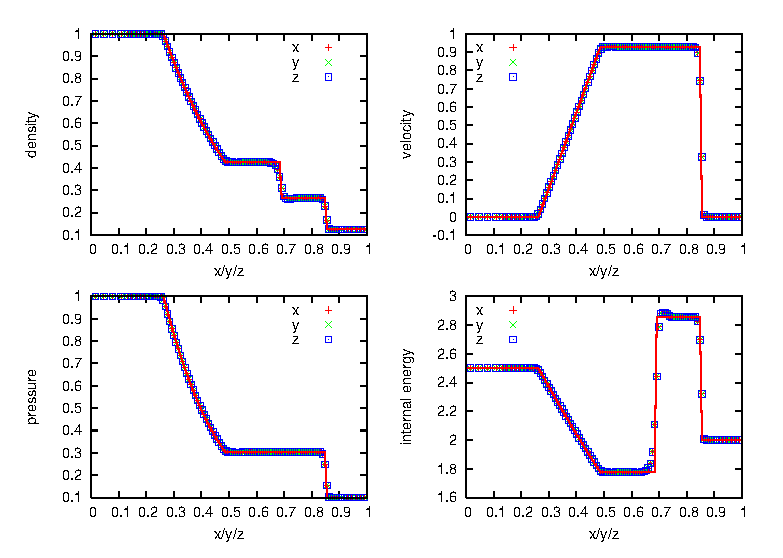
\includegraphics[width=4.75in]{CastroVerification/sod_3d_ppm0}
\caption{\label{fig:sod_ppm0} Castro solution for Sod's problem run in 3-d,
  with the piecewise-linear Godunov method with limiters,
  along the $x$, $y$, and $z$ axes.  A coarse grid of 32 zones in the
  direction of propagation, with 2 levels of refinement was used.  The
  analytic solution appears as the red line.}
\end{figure}

Figure~\ref{fig:sod} shows the Castro solution using the newest PPM limiters
compared to the analytic 
solution, showing the density, velocity, pressure, and internal energy.
Figure~\ref{fig:sod_ppm0} is the same as Figure~\ref{fig:sod},
but with the piecewise-linear Godunov method with limiters, 
shown for comparison.

The {\tt Verification} subdirectory includes the analytic solution for
the Sod problem {\tt sod-exact.out}, with $\gamma = 1.4$.  1-d slices
can be extracted from the Castro plotfile using the {\tt fextract} tool
from {\tt fParallel/data\_processing/}.  The steps to
generate this verification plot with Castro are:
\begin{enumerate}
\item in {\tt Exec/Sod}, build the Castro executable in 3-d
\item run the Sod problem with Castro in the $x$, $y$, and $z$ directions: \\
 {\tt ./Castro3d.Linux.Intel.Intel.ex inputs-sod-x} \\
 {\tt ./Castro3d.Linux.Intel.Intel.ex inputs-sod-y} \\
 {\tt ./Castro3d.Linux.Intel.Intel.ex inputs-sod-z}
\item build the {\tt fextract} tool in {\tt fParallel/data\_processing}
\item run {\tt fextract} on the Castro output to generate 1-d slices
 through the output: \\
 {\tt fextract3d.Linux.Intel.exe -d 1 -s sodx.out -p sod\_x\_plt00034} \\
 {\tt fextract3d.Linux.Intel.exe -d 2 -s sody.out -p sod\_y\_plt00034} \\
 {\tt fextract3d.Linux.Intel.exe -d 3 -s sodz.out -p sod\_z\_plt00034}
\item copy the {\tt sodx/y/z.out} files into the {\tt Verification} directory.
\item in {\tt Verification} run the gnuplot script {\tt sod\_3d.gp} as: \\
 {\tt gnuplot sod\_3d.gp} \\
 This will produce the figure {\tt sod\_3d.eps}.
\end{enumerate}

\subsubsection{Double Rarefaction}

The double rarefaction is the ``Test 2'' problem described by Toro
\cite{toro:1997}, Chapter 6.  In this test, the center of the domain
is evacuated as two rarefaction waves propagate in each direction, outward
from the center.  It is difficult to get the internal energy to 
behave at the center of the domain because we are creating a vacuum.
The initial conditions are:
\begin{equation}
\begin{array}{l}
\rho_L = 1 \\
u_L = -2 \\
p_L = 0.4
\end{array}
\qquad
\begin{array}{l}
\rho_R = 1 \\
u_R = 2 \\
p_R = 0.4
\end{array}
\end{equation}
The {\tt gamma\_law} equation of state is used with $\gamma = 1.4$.
The system is evolved until $t = 0.15$~s.  Setups for 1-, 2-, and 3-d
are provided.  The following inputs files and probin files setup the
Sod's problem:
\begin{table*}[h]
\centering
\begin{tabular}{|l|l|l|} \hline
\multicolumn{1}{|c}{\em inputs file} &  \multicolumn{1}{|c}{\em probin file} & \multicolumn{1}{|c|}{\em description} \\
\hline
{\tt inputs-test2-x} & {\tt probin-test2-x} & Double rarefaction problem along $x$-direction \\
{\tt inputs-test2-y} & {\tt probin-test2-y} & Double rarefaction problem along $y$-direction \\
{\tt inputs-test2-z} & {\tt probin-test2-z} & Double rarefaction problem along $z$-direction \\
\hline
\end{tabular}
\label{Table:Sod}
\end{table*}

We use a CFL number of 0.8, an initial
timestep shrink ({\tt castro.init\_shrink}) of 0.1, and the maximum factor by which
the timestep can increase ({\tt castro.change\_max}) of 1.05.  The PPM
solver with the new limiters are used.
\begin{figure}[h]
\centering
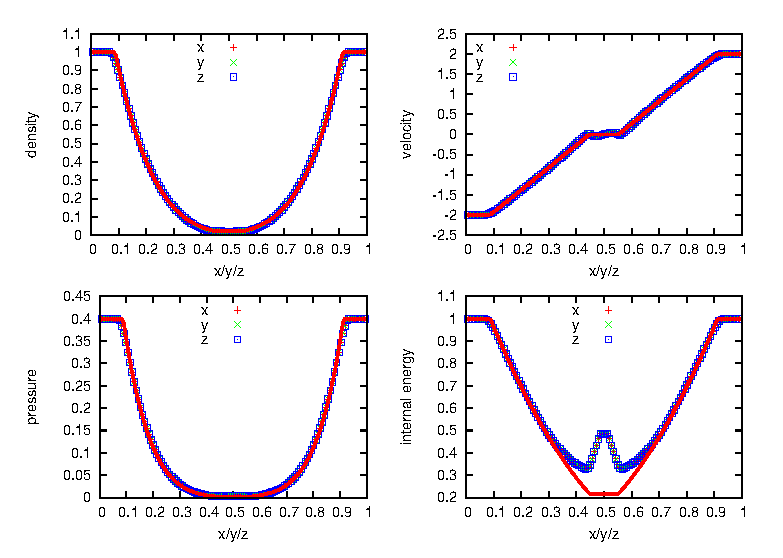
\includegraphics[width=5.0in]{CastroVerification/test2_3d}
\caption{\label{fig:test2} Castro solution for the double rarefaction
  problem run in 3-d, along the $x$, $y$, and $z$ axes.  A coarse grid
  of 32 zones in the direction of propagation, with 2 levels of
  refinement was used.  The analytic solution appears as the red
  line.}
\end{figure}

Figure~\ref{fig:test2} shows the Castro output, run along all 3
coordinate axes in 3-d, compared to the analytic solution.  

The comparison to the analytic solution follows the same procedure as
described for the Sod's problem above.  The gnuplot script {\tt
  test2\_3d.gp} will generate the figure, from the 1-d slices created by
{\tt fextract} named {\tt test2x.out}, {\tt test2y.out}, and {\tt test2z.out}.

\subsubsection{Strong Shock}

The strong shock test is the ``Test 3'' problem described by Toro
\cite{toro:1997}, Chapter 6.  In this test, a large pressure jump
at the initial interface creates a very strong rightward moving
shock, followed very closely by a contact discontinuity.
The initial conditions are:
\begin{equation}
\begin{array}{l}
\rho_L = 1 \\
u_L = 0 \\
p_L = 1000
\end{array}
\qquad
\begin{array}{l}
\rho_R = 1 \\
u_R = 0 \\
p_R = 0.01
\end{array}
\end{equation}
The {\tt gamma\_law} equation of state is used with $\gamma = 1.4$.
The system is evolved until $t = 0.012$~s.  Setups for 1-, 2-, and 3-d
are provided.  The following inputs files and probin files setup the
Sod's problem:
\begin{table*}[h]
\centering
\begin{tabular}{|l|l|l|} \hline
\multicolumn{1}{|c}{\em inputs file} &  \multicolumn{1}{|c}{\em probin file} & \multicolumn{1}{|c|}{\em description} \\
\hline
{\tt inputs-test3-x} & {\tt probin-test3-x} & Strong shock problem along $x$-direction \\
{\tt inputs-test3-y} & {\tt probin-test3-y} & Strong shock problem along $y$-direction \\
{\tt inputs-test3-z} & {\tt probin-test3-z} & Strong shock problem along $z$-direction \\
\hline
\end{tabular}
\label{Table:Sod}
\end{table*}

We use a CFL number of 0.9, an initial
timestep shrink ({\tt castro.init\_shrink}) of 0.1, and the maximum factor by which
the timestep can increase ({\tt castro.change\_max}) of 1.05.  The PPM
solver with the new limiters are used.

\begin{figure}[t]
\centering
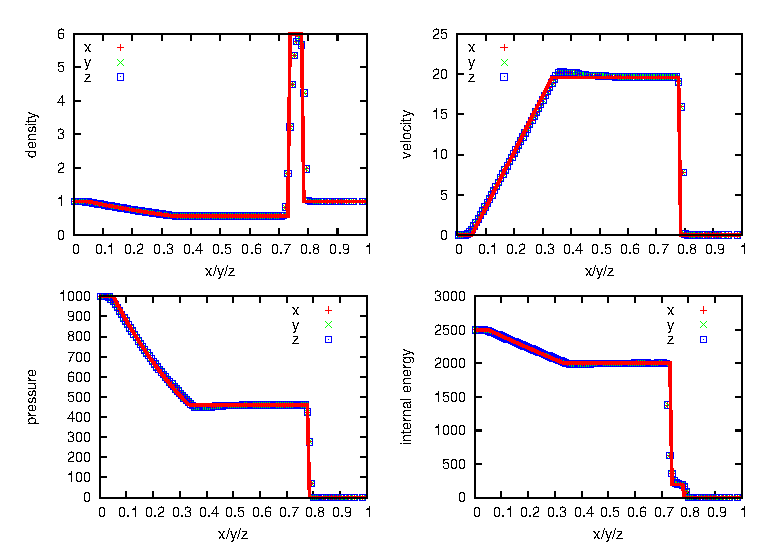
\includegraphics[width=5.0in]{CastroVerification/test3_3d}
\caption{\label{fig:test3} Castro solution for the strong shock
  problem run in 3-d, along the $x$, $y$, and $z$ axes.  A coarse grid
  of 32 zones in the direction of propagation, with 2 levels of
  refinement was used.  The analytic solution appears as the red
  line.}
\end{figure}

Figure~\ref{fig:test3} shows the Castro output, run along all 3
coordinate axes in 3-d, compared to the analytic solution.  

The comparison to the analytic solution follows the same procedure as
described for the Sod's problem above.  The gnuplot script {\tt
  test3\_3d.gp} will generate the figure, from the 1-d slices created by
{\tt fextract} named {\tt test3x.out}, {\tt test3y.out}, and {\tt test3z.out}.


\subsection{Sedov Problem}

The Sedov (or Sedov-Taylor) blast wave is a standard hydrodynamics
test problem.  A large amount of energy is placed into a very small
volume, driving a spherical (or cylindrical in 2-d Cartesian
coordinates) blast wave.  Analytic solutions were found by Sedov
\cite{sedov:1959}.  

A cylindrical blast wave (e.g.\ a point explosion in a 2-d plane) can
be modeled in 2-d Cartesian coordinates.  A spherical blast wave can
be modeled in 1-d spherical, 2-d axisymmetric (cylindrical $r$-$z$), or 3-d
Cartesian coordinates.  This provides a good test on the geometric
factors in the hydrodynamics solver.
We use a publically available code, {\tt sedov3.f}
\cite{timmes_sedov_code}, to generate the analytic solutions.

The Castro implementation of the Sedov problem is in {\tt Exec/Sedov}.
A number of different inputs/probin files are provided, corresponding
to different Sedov/Castro geometries.  The main ones are:

\begin{table*}[h]
\centering
{\small
\begin{tabular}{|l|l|p{2.25in}|} \hline
\multicolumn{1}{|c}{\em inputs file} &  \multicolumn{1}{|c}{\em probin file} & \multicolumn{1}{|c|}{\em description} \\
\hline
{\tt inputs.1d.sph} & {\tt probin.1d.sph} & Spherical Sedov explosion modeled in 1-d spherical coordinates \\[2mm]
%
{\tt inputs.2d.sph\_in\_cylcoords} & {\tt probin.2d.sph\_in\_cylcoords} & Spherical Sedov explosion modeled in 2-d cylindrical (axisymmetric) coordinates \\[2mm]
%
{\tt inputs.2d.cyl\_in\_cartcoords} & {\tt probin.2d.cyl\_in\_cartcoords} & Cylindrical Sedov explosion modeled in 2-d Cartesian coordinates \\[2mm]
%
{\tt inputs.3d.sph} & {\tt probin.3d.sph} & Spherical Sedov explosion modeled in 3-d Cartesian coordinates \\
\hline
\end{tabular}
\caption{\label{table:sedov_inputs} Sedov inputs files}
} % end small
\label{Table:Sod}
\end{table*}

In the Sedov problem, the explosion energy, $E_\mathrm{exp}$ (in units 
of energy, not energy/mass or energy/volume)
is to be deposited into a single point, in a medium of uniform ambient
density, $\rho_\mathrm{ambient}$, and pressure, $p_\mathrm{ambient}$.
Initializing the problem can be difficult because the small volume is
typically only a cell in extent.  This can lead to grid imprinting in
the solution.  A standard solution (see for example \cite{omang:2006}
and the references therein)
is to convert the explosion energy into a pressure contained within a
certain volume, $V_\mathrm{init}$, of radius $r_\mathrm{init}$ as
\begin{equation}
p_\mathrm{init} = \frac{(\gamma - 1) E_\mathrm{exp}}{V_\mathrm{init}} \enskip .
\end{equation}
This pressure is then deposited in all of the cells where $r <
r_\mathrm{init}$.  

To further minimize any grid effects, we do subsampling
in each zone: each zone is divided it into $N_\mathrm{sub}$ subzones in each
coordinate direction, each subzone is initialized independently, and
then the subzones are averaged together (using a volume weighting for
spherical or cylindrical/axisymmetric Castro grids) to determine the
initial state of the full zone.

For these runs, we use $\rho_\mathrm{ambient} = 1$,
$p_\mathrm{ambient} = 10^{-5}$, $E_\mathrm{exp} = 1$, $r_\mathrm{init}
 = 0.01$, and $N_\mathrm{sub} = 10$.  A base grid with 32 zones in each
coordinate direction plus 3 levels of refinement is used (the finest
mesh would coorespond to 256 zones in a coordinate direction).  The
domain runs from 0 to 1 in each coordinate direction.




Analysis routines for the Sedov problem are provided in {\tt
  fParallel/data\_processing/Castro\_hydro}.  These routines will
average the Castro solution over angles, using the proper geometric
weighting, to produce an average profile as a function of radius.
The following routines correspond to the inputs files described above:
\begin{table*}[h]
\centering
{\small
\begin{tabular}{|l|l|} \hline
\multicolumn{1}{|c}{\em inputs file} &  \multicolumn{1}{|c|}{\em analysis routine} \\
\hline
{\tt inputs.1d.sph} & {\tt fsedov1d.f90} \\
%
{\tt inputs.2d.sph\_in\_cylcoords} & {\tt fsedov2d\_sph\_in\_cylcoords.f90} \\
%
{\tt inputs.2d.cyl\_in\_cartcoords} & {\tt fsedov2d\_cyl\_in\_cartcoords.f90} \\
%
{\tt inputs.3d.sph} & {\tt fsedov3d\_sph.f90} \\
\hline
\end{tabular}
} % end small
\caption{\label{table:fsedov} Analysis routines for Sedov}
\end{table*}

\subsubsection{Spherical Blast Wave}

A spherical Sedov explosion can be modeled in 1-d spherical, 2-d
cylindrical (axisymmetric), or 3-d Cartesian coordinates, using the
inputs files described in Table~\ref{table:sedov_inputs}.  A 1-d radial
profile can be extracted using the appropriate {\tt fsedov} routine,
as listed in Table~\ref{table:fsedov}.  For example, to run and process
the 2-d cylindrical Sedov explosion, one would do:
\begin{enumerate}
\item in {\tt Exec/Sedov}, build the Castro executable in 2-d
\item run the spherical Sedov problem with Castro in 2-d cylindrical coordinates: \\
 {\tt ./Castro2d.Linux.Intel.Intel.ex inputs.2d.sph\_in\_cylcoords} 
\item build the {\tt fsedov2d\_sph\_in\_cylcoords} tool in {\tt fParallel/data\_processing}
\item run {\tt fsedov2d\_sph\_in\_cylcoords} on the Castro output to generate 1-d radial
 profiles: \\
 {\tt fsedov2d\_sph\_in\_cylcoords.Linux.Intel.exe -s sedov\_2d\_sph\_in\_cyl.out $\mathtt{\backslash}$ } \\
 $~~~~~${\tt -p sedov\_2d\_sph\_in\_cyl\_plt00246} 
\end{enumerate}
A similar procedure can be used for the 1-d and 3-d spherical Sedov
explosions (with the output named {\tt sedov\_1d\_sph.out} and {\tt
  sedov\_3d\_sph.out} respectively).  Once this is done, the {\tt
  sedov\_sph.gp} gnuplot script can be used to make a plot comparing
the 3 solutions to the analytic solution, {\tt spherical\_sedov.dat}.

Figure~\ref{fig:sedov_sph} shows the comparison of the 3 Castro
spherical Sedov explosion simulations to the analytic solution.

\begin{figure}[t]
\centering
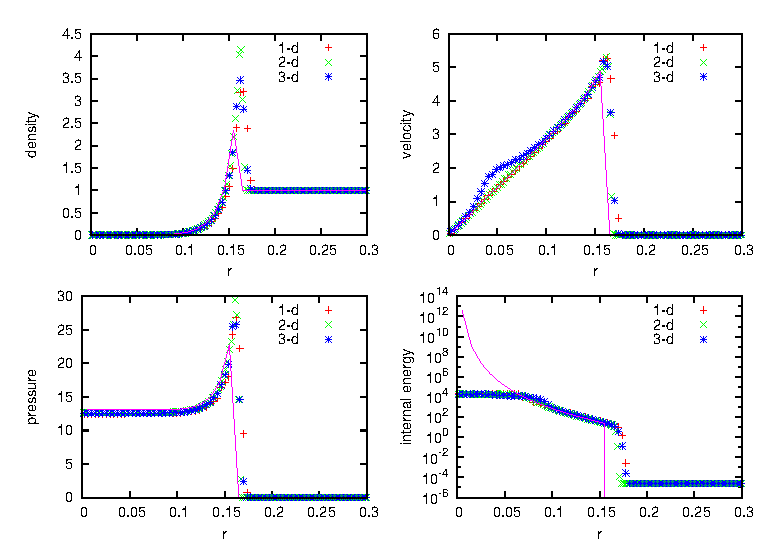
\includegraphics[width=5.0in]{CastroVerification/sedov_sph}
\caption{\label{fig:sedov_sph} Castro solution for the Sedov blast wave problem
  run in 1-d spherical, 2-d axisymmetric, and 3-d Cartesian coordinates.
  Each of these geometries produces a spherical Sedov explosion.}
\end{figure}


\subsubsection{Cylindrical Blast Wave}

\begin{figure}[h]
\centering
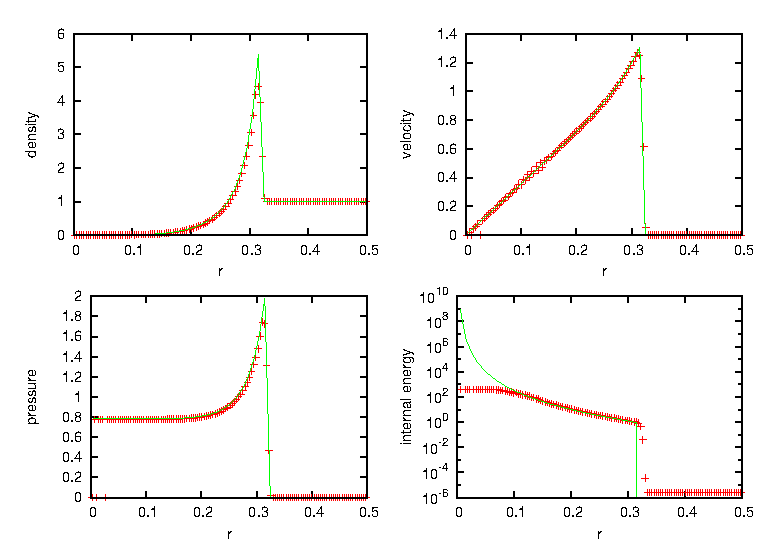
\includegraphics[width=5.0in]{CastroVerification/sedov_cyl}
\caption{\label{fig:sedov_cyl} Castro solution for the Sedov blast wave problem
  run in 2-d Cartesian coordinates.  This corresponds to a cylindrical
  Sedov explosion.}
\end{figure}

\subsection{Rayleigh-Taylor}
2D.  Domain size 0.5 by 1.0.  256 by 512 cells, single level
calculation.  Periodic in x, solid walls on top and bottom in y.
Gamma law gas with $\gamma=1.4$, no reactions.  Zero initial velocity.
Constant $|\gb|=1$.  The density profile is essentially $\rho=1$ on
bottom, $\rho=2$ on top, but with a perturbation.  A single-mode
perturbation is constructed as:
\begin{equation}
\tilde y(x) = 0.5 + 0.01 \frac{\cos(4\pi x) + \cos(4\pi(L_x - x))}{2}
\end{equation}
We note that the symmetric form of the cosine is done to ensure that 
roundoff error does not introduce a left-right asymmetry in the problem.
Without this construction, the R-T instability will lose its symmetry
as it evolves.  This then applied to the interface with a tanh profile
to smooth the transition between the high and low density material:
\begin{equation}
\rho(x,y) = 1 + 0.5\left[1+\tanh\left(\frac{y-\tilde y(x)}{0.005}\right)\right]
\end{equation}
Hydrostatic pressure with $p=5.0$ at bottom of domain, assuming
$\rho=1$ on the lower half of the domain, and $\rho=2$ on the upper
half and no density perturbation.  We run to $t=2.5$ with piecewise
linear, old PPM, and new PPM.  CFL=0.9.  See Figure \ref{fig:RT}.
\begin{figure}[h]
\centering
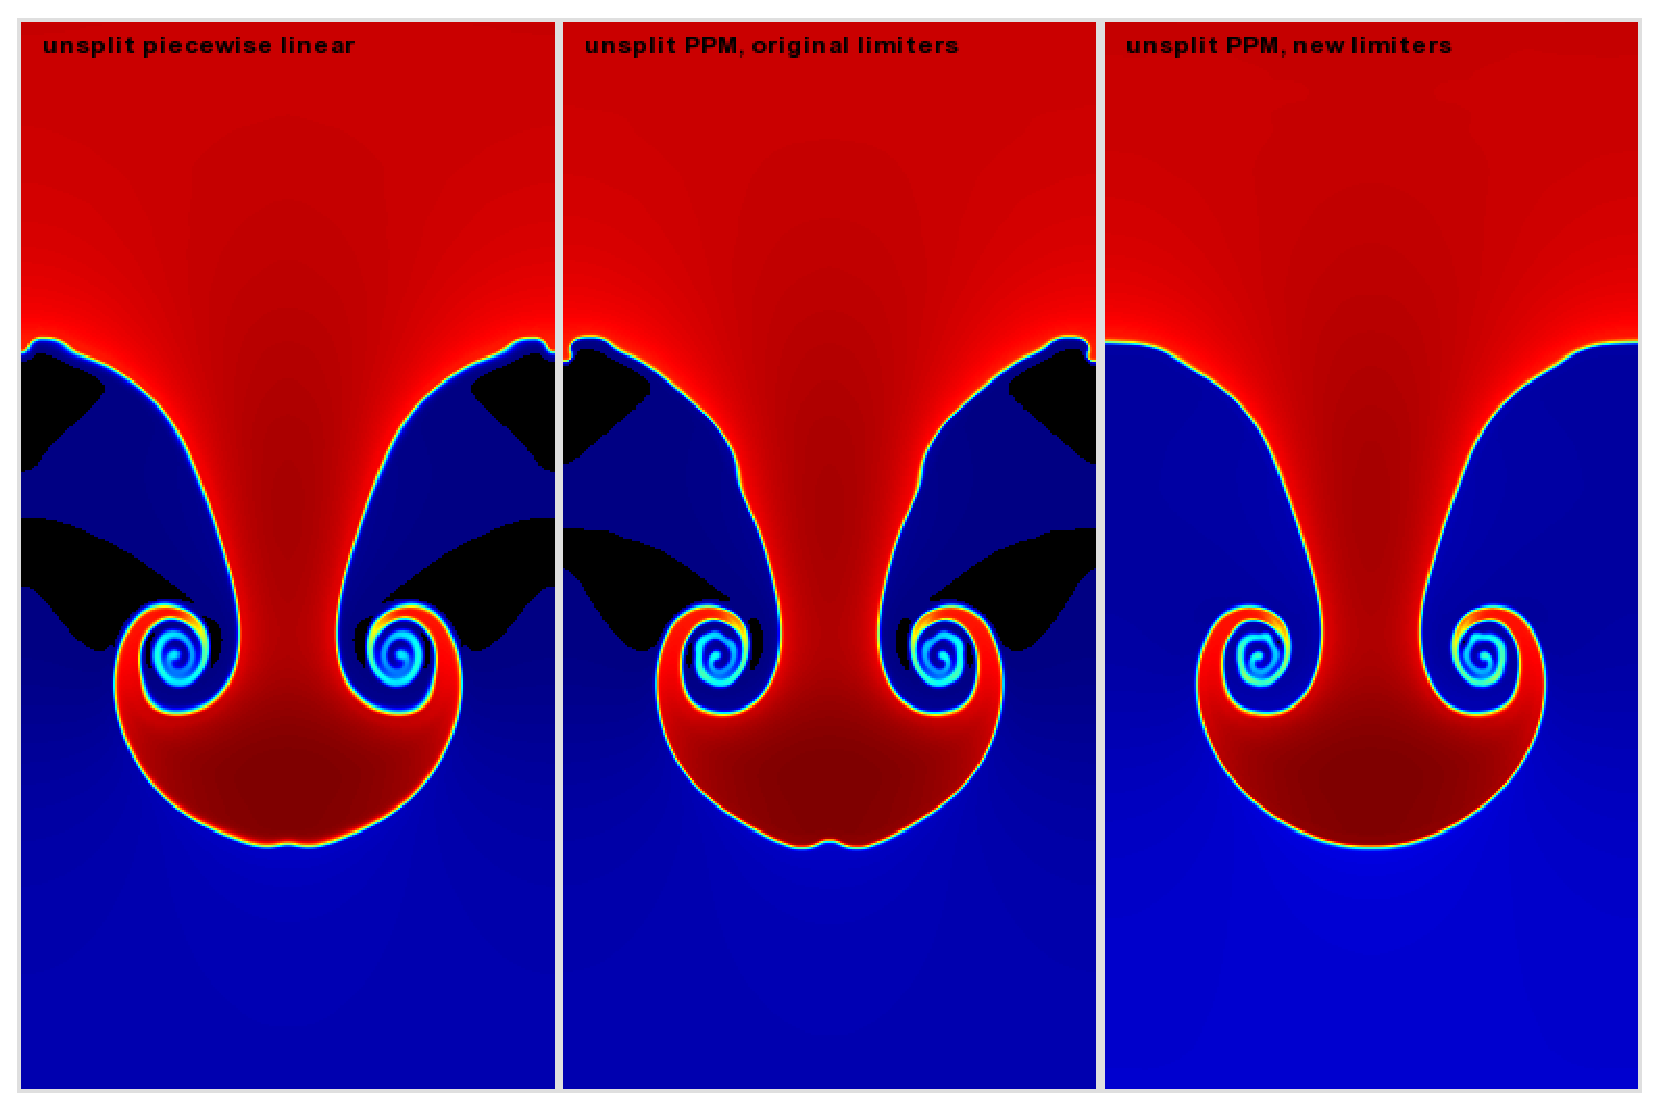
\includegraphics[width=6.5in]{CastroVerification/RT_ppm_type}
\caption{\label{fig:RT}Rayleigh-Taylor with different PPM types.}
\end{figure}

%%%%%%%%%%%%%%%%%%%%%%%%%%%%%%%%%%%%%%%%%%%%%%%%%%%%%%%%%%%%%%%%%%%%%%%%%%%%%%%
\section{Gravity Test Problems}



%%%%%%%%%%%%%%%%%%%%%%%%%%%%%%%%%%%%%%%%%%%%%%%%%%%%%%%%%%%%%%%%%%%%%%%%%%%%%%%
\section{Radiation Test Problems}

There are two photon radiation solvers in Castro---a gray solver and a
multigroup solver.  The gray solver follows the algorithm outlined
in \cite{howellgreenough:2003}.  We use the notation described in that
paper.  In particular, the radiation energy equation takes the form
of:
\begin{equation}
\frac{\partial E_R}{\partial t} = 
 \nabla \cdot \left ( \frac{c \lambda(E_R)}{\kappa_R} \nabla E_R \right ) +
 \kappa_P (4 \sigma T^4 - c E_R )
\end{equation}
Here, $E_R$ is the radiation energy density, $\kappa_R$ is the
Roseland-mean opacity, $\kappa_P$ is the Planck-mean opaciy, and
$\lambda$ is a quantity $\le 1/3$ that is subjected to limiting to
keep the radiation field causal.  Castro allows for $\kappa_R$
and $\kappa_P$ to be set independently as power-laws.

\subsection{Light Front}

The light front problem tests the ability of the radiation solver to
operate in the free-streaming limit.  A radiation front is
estabilished by initializing one end of the computational domain with
a finite radiation field, and zero radiation field everywhere else.
The speed of propagation of the radiation front is keep in check by
the flux-limiters, to prevent it from exceeding $c$.


\subsection{Diffusion of a Gaussian Pulse}

The diffusion of a Gaussian pulse problem tests the diffusion term in
the radiation energy equation.  The radiation energy density is 
initialized at time $t = t_0$ to a Gaussian distribution:
\begin{equation}
E_R = (E_R)_0 \exp \left \{ - \frac{1}{4 D t_0} |r - r_0|^2 \right \} \enskip .
\end{equation}
As the radiation diffuses, the overall distribution will remain 
Gaussian, with the time-dependent solution of:
\begin{equation}
E_R = (E_R)_0 \frac{t_0}{t_0 + t} \exp \left \{ -\frac{1}{4 D (t_0 + t)} |r - r_0|^2 \right \}
\end{equation}


\subsection{Radiation Source Problem}

The radiation source problem tests the coupling between the radiation
field and the gas energy through the radiation source term.  The
problem begins with the radiation field and gas temperature out of
equilibrium.  If the gas is too cool, then the radiation field will
heat it.  If the gas is too hot, then it will radiate and cool.  In
each case, the gas energy and radiation field will evolve until
thermal equilibrium is achieved.

Our implementation of this problem follows that of
\cite{swestymyra:2009}.

\begin{figure}[h]
\centering
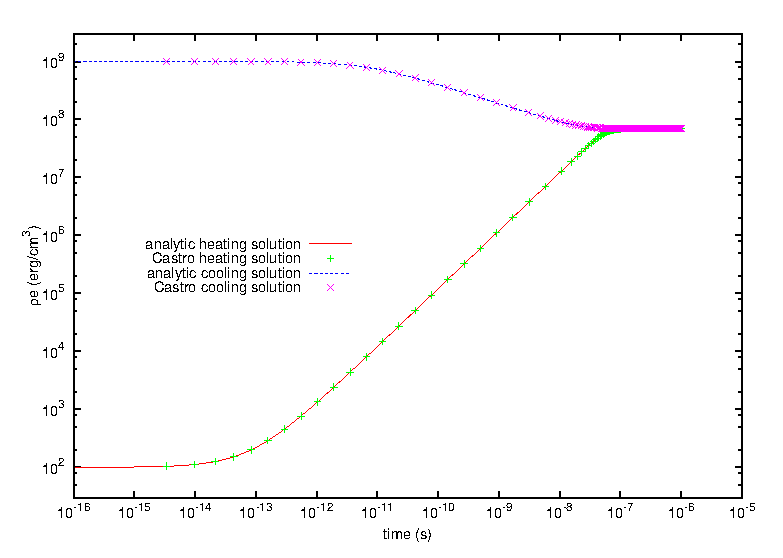
\includegraphics[width=5.0in]{CastroVerification/radiating_source}
\caption{\label{fig:radsource} Castro solution for radiating source
  test problem.  Heating and cooling solutions are shown as a function
  of time, compared to the analytic solution.  The gray photon solver
  was used.}
\end{figure}


\subsection{Radiating Sphere}

The radiating sphere is a multigroup radiation test problem.  A hot
sphere is centered at the origin in a spherical geometry.  The
spectrum from this sphere follows a Planck distribution.  The ambient
medium is at a much lower temperature.  A frequency-dependent opacity
makes the domain optically thin for high frequecies and optically
thick for low frequency.  At long times, the solution will be a
combination of the blackbody radiation from the ambient medium plus
the radiation that propagated from the hot sphere.  An analytic
solution exists \cite{graziani:2008} which gives the radiation energy
as a function of energy group at a specified time and distance from
the radiating sphere.

Our implementation of this problem is in {\tt Exec/RadSphere} and
follows that of \cite{swestymyra:2009}.  The routine that computes
the analytic solution is provided as {\tt analytic.f90}.

\begin{figure}[h]
\centering
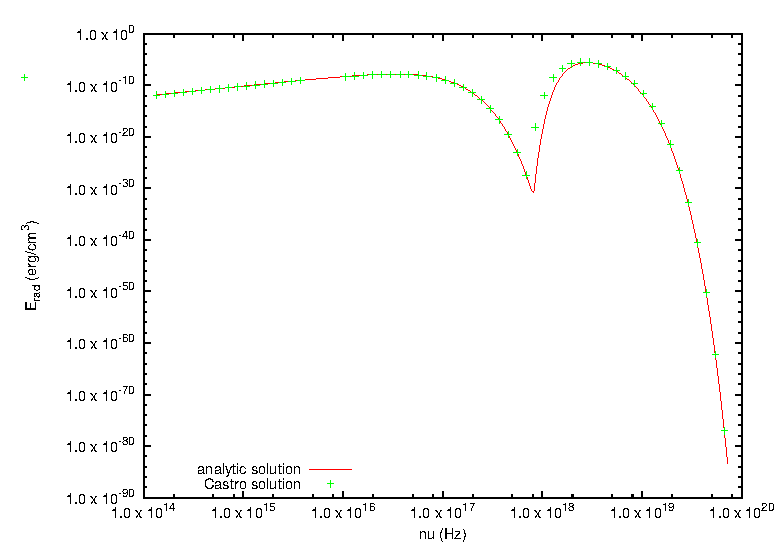
\includegraphics[width=5.0in]{CastroVerification/radiating_sphere}
\caption{\label{fig:radsphere} Castro solution for radiating sphere problem,
  showing the radiation energy density as a function of energy group.
  This test was run with 64 photon energy groups.}
\end{figure}


\section{Regression Testing}

An automated regression test suite for Castro (or any BoxLib-based
code) written in Python exists in {\tt Parallel/util/regtests/} as
{\tt test.py}.  The test suite consists of a set of problem
definitions (the Castro problem + their inputs/probin files, etc.).
When the suite is run the first time, the plotfiles created at the end
of each problem's executation is stored as a benchmark.  After this
initialization, each subsequent run of the test suite compares the
current output of the code, level-by-level and zone-by-zone to the
stored benchmarks (using the {\tt fcompare.f90} routine in {\tt
  fParallel/data\_processing/}).  Any differences are flagged as
errors.  A web page report is generated by the test suite and provides
a history of the regression testing.  Single-processor and parallel
test problems, compilation tests, and testing restarting from a
checkpoint file are supported.

\begin{figure}[t]
\centering
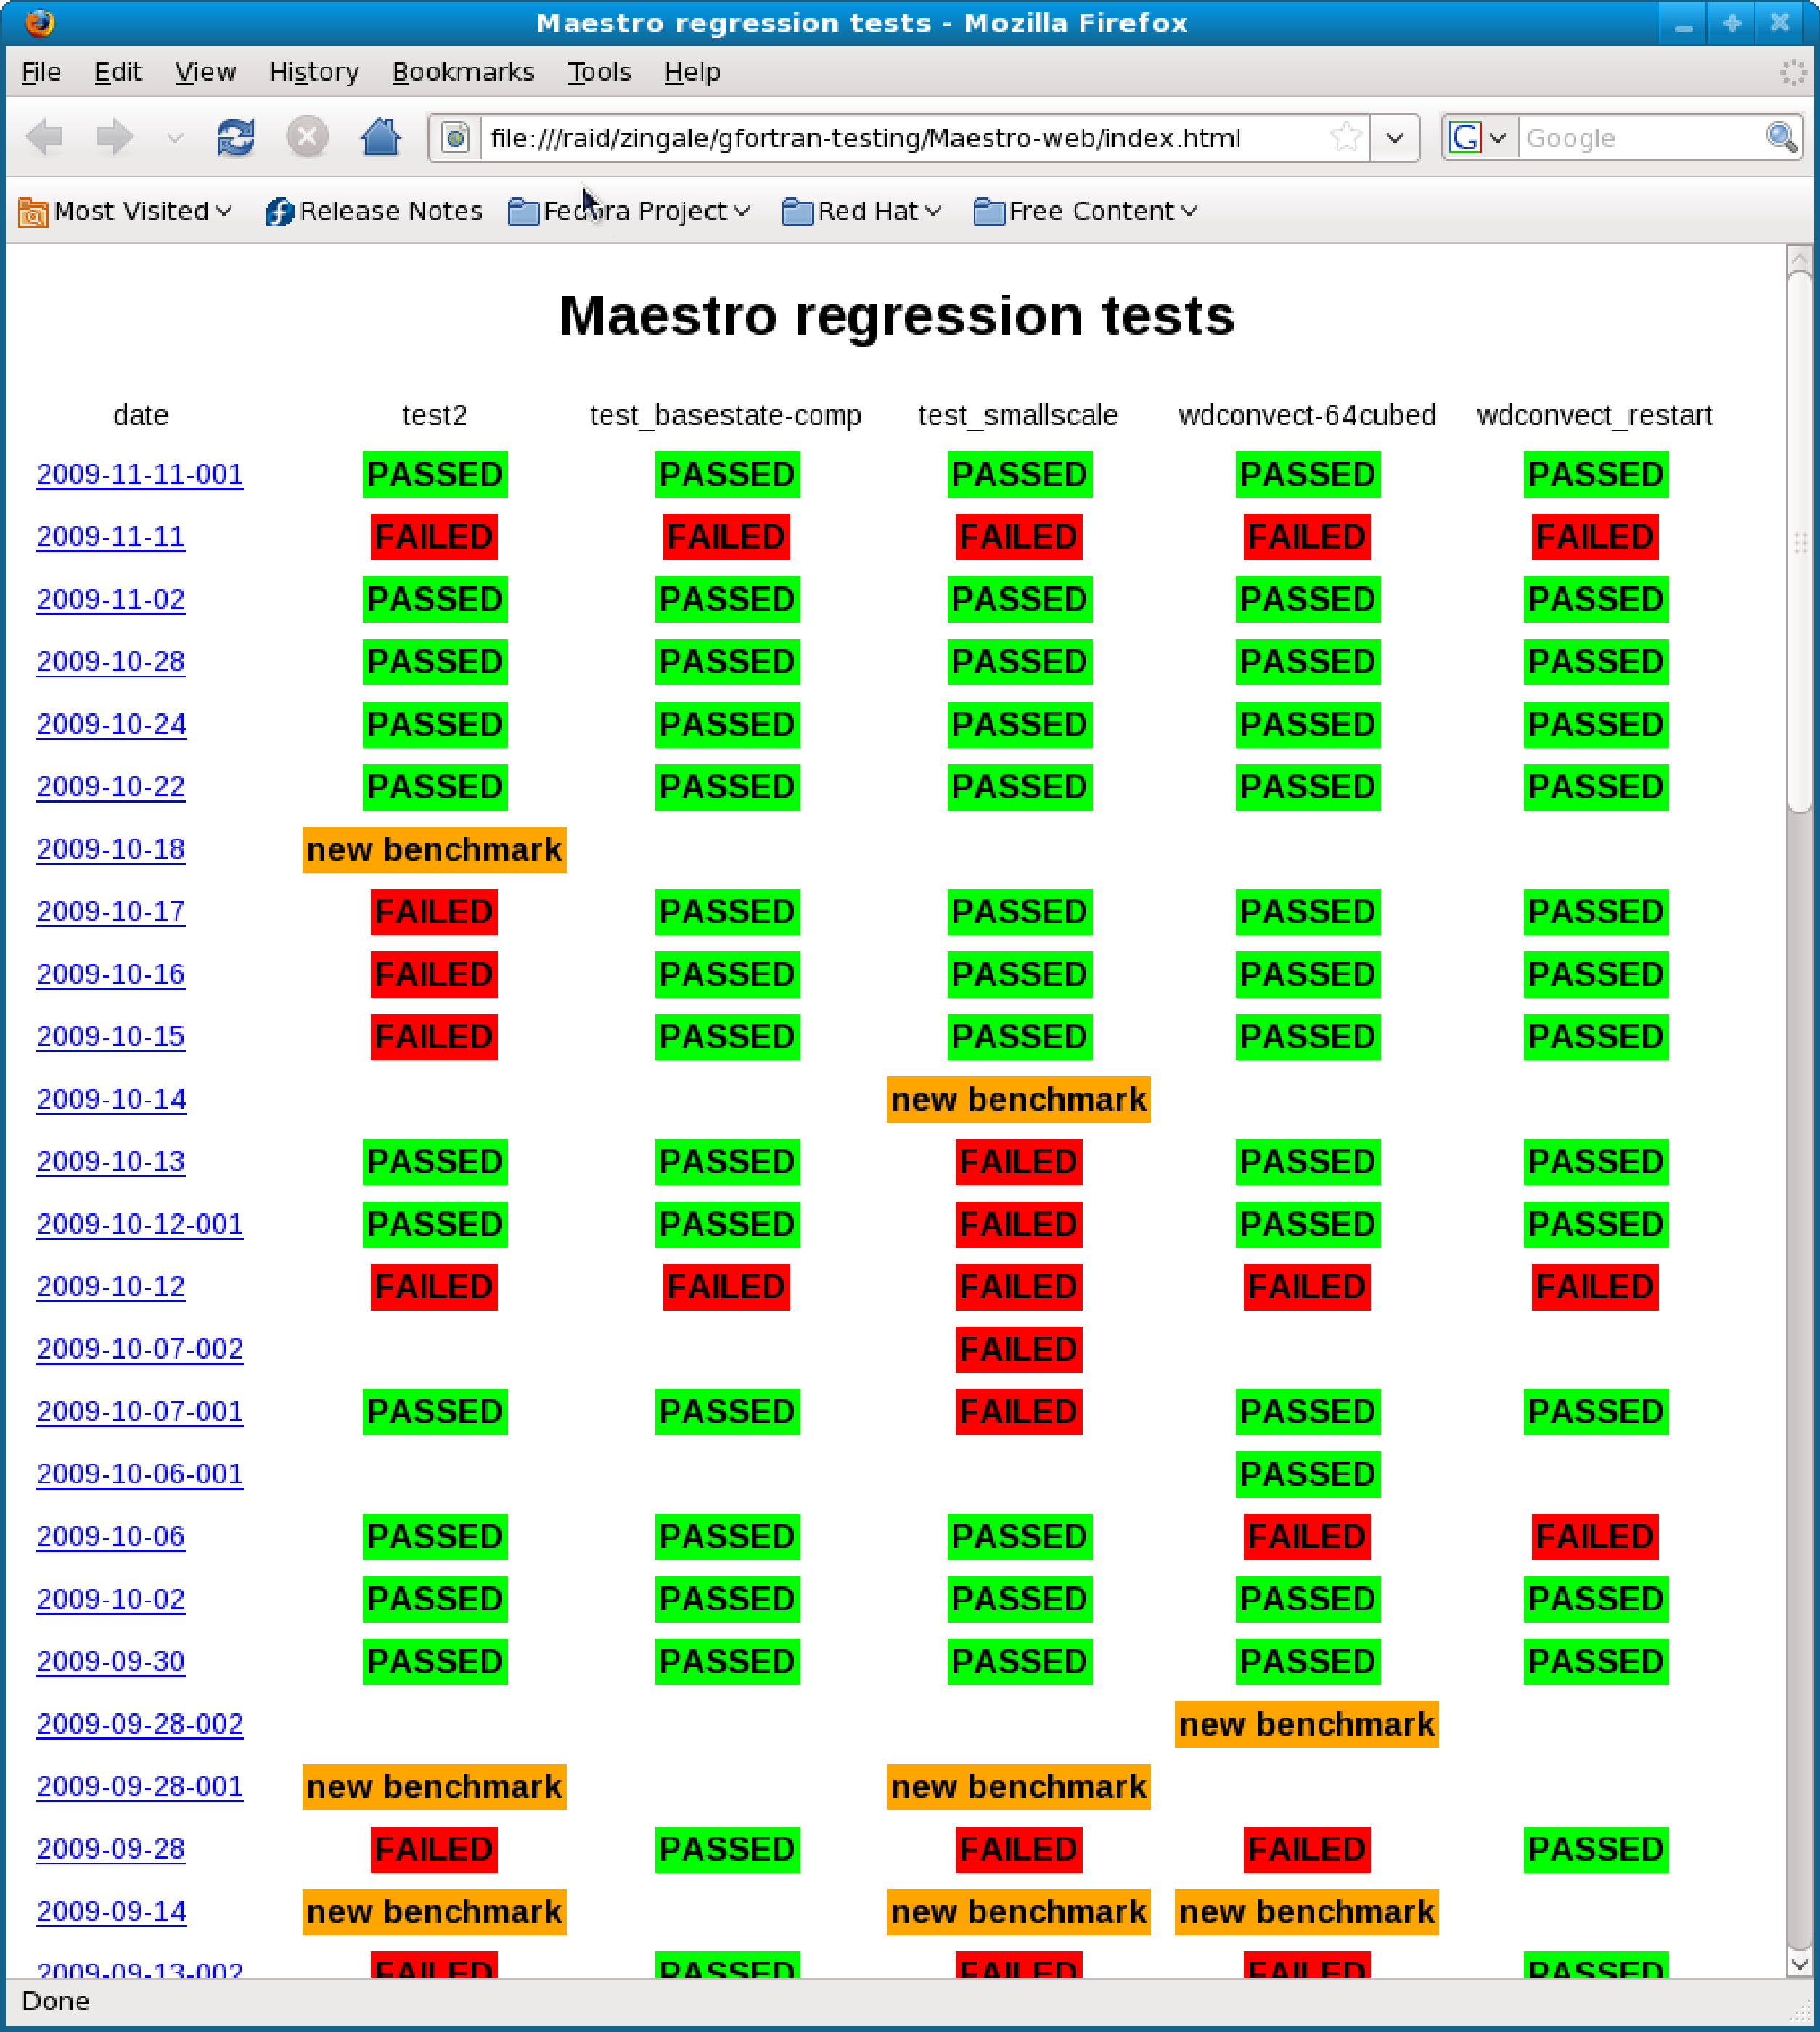
\includegraphics[width=5.0in]{CastroVerification/test_suite_main}
\caption{\label{fig:test_suite_main} Main test suite results page.  Each 
row indicates a single test suite run, arranged by date, and each column
indicates a different test problem.  Note: this page is from the {\tt Maestro}
code, but a {\tt Castro} test suite run will produce similar output.}
\end{figure}

\subsection{Test Suite Inputs File}

The inputs file for the test suite separates the problems into blocks.
The header of a problem block has the form {\tt [problem-name]}.
Beneath each problem block, there are a number of options set for each
problem.  A separate heading, {\tt [main]}, is used for the suite-wide
options.

An example of the {\tt main} block from {\tt Castro-tests.ini} is:
\begin{verbatim}
[main]
sourceDir      = /work/zingale/test/CASTRO/
testTopDir     = /work/zingale/test/CASTRO/
compareToolDir = /work/zingale/test/CASTRO/fParallel/data_processing/
helmeosDir     = /work/zingale/test/CASTRO/fParallel/extern/EOS/helmeos/

sourceTree = Parallel

COMP = Intel
FCOMP = Intel

suiteName = Castro

MPIcommand = mpiexec -host @host@ -n @nprocs@ @command@
MPIhost = node1
\end{verbatim}

The first group of options define the necessary paths.
Here, {\tt sourceDir} points to the top-level directory, which is
expected to contain the {\tt Parallel} and {\tt fParallel} subdirectories.
{\tt testTopDir} refers to the directory that the suite should use as
its root directory for output---usually this is the same as {\tt sourceDir}.
The {\tt fcompare.f90} comparison tool is expected to be found in
{\tt compareToolDir}.  Finally, {\tt helmeosDir} lists the path to the
{\tt helm\_table.dat} file used by the general stellar equation of state.

Next, we set {\tt sourceTree} to {\tt Parallel}, indicating that
Castro is built using the C++ BoxLib framework.  ({\tt Maestro} uses
the Fortran 95 BoxLib framework, and therefore would set {\tt
  sourceTree} to {\tt fParallel}).  This option tells the test suite
what build system to use.

{\tt COMP} and {\tt FCOMP} tell the test suite which C++ and Fortran
compilers to use.  These override what is listed in any {\tt
  GNUmakefile} to ensure that the compiler stays consistent in the
tests.

The {\tt suiteName} option simply tells the test suite what name to
prefix to the output directories.  It does not need to match the
program name.  

Finally, {\tt MPIcommand} lists the generic manner in which to run an
MPI program on the target system.  The string {\tt @host@} in the
{\tt MPIcommand} will be substituted by the {\tt MPIhost} string by
the test suite.  Similarly the {\tt @nprocs@} string will be
substituted by the number of processors, which is set on a
problem-by-problem basis.  Finally, the {\tt MPIcommand} should
include the string {\tt @command@}, which is where the Castro
executable and inputs file will be substituted.  For single processor
runs, these options are ignored.

Each problem to be run by the test suite gets its own block.  For
example, a Sod's problem test might look like:

\begin{verbatim}
[Sod-x]
buildDir = Parallel/Castro/Exec/Sod/
inputFile = inputs-sod-x
probinFile = probin-sod-x
needs_helmeos = 0
dim = 3
restartTest = 0
useMPI = 0
compileTest = 0
doVis = 0
\end{verbatim}

Here {\tt Sod-x} contained inside the {\tt []} is the name of the problem, as the 
test suite will refer to it.  {\tt buildDir} is the path beneath {\tt sourceDir} 
where the {\tt make} command should be executed.  The inputs file and probin file
are given by {\tt inputFile} and {\tt probinFile}, which should be relative
to the {\tt buildDir}.  The dimensionality is specified by {\tt dim}.

A number of options are available:
\begin{itemize}
\item  If the general stellar equation of state is
used, then {\tt needs\_helmeos} should be set to {\tt 1} to ensure that the
EOS table is copied into the run directory.  

\item If the test is to be run in parallel,
the {\tt useMPI} should be {\tt 1} and {\tt numprocs} should give the number
of processors.  

\item To test the compilation of the problem only (and skip running),
set {\tt compileTest} to {\tt 1}.  

\item To test the ability of the code to restart, set {\tt restartTest} to
{\tt 1}.  Also set {\tt restartFileNum} to the number of the checkpoint file to restart
from.  The suite will run the problem as usual and then restart from the specified
checkpoint and run to completion again.  The output from the initial run will
then be compared to the output from the restart.  In a restart test, there
is no stored benchmark.

\item To add a simple visualization to the test suite webpage, set
  {\tt doVis} to {\tt 1}, and set {\tt visVar} to the name of the
  plotfile variable to visualize.  An image of that field from the
  last plotfile will be appended to the problem's test webpage.

\end{itemize}



\subsection{Initializing the Test Suite}

The first time you run the test suite there are no benchmark files to compare to.
Once you generate an inputs file, as described above, you would simply run the
suite as: \\
$~~~~~${\tt ./test.py --make\_benchmarks "initial run" ./Castro\_tests.ini} \\
The string following {\tt --make\_benchmarks} is simply a comment that will
be added to the web report.
This command creates three output directories, using the {\tt suiteName} as the prefix.
\begin{itemize}
\item {\tt suiteName-tests} is where the tests are run.  Each time the test
 suite is run, a subdirectory, based on the date, is created, with a subdirectory
 for each test.  All the files necessary to run the test are copied into the
 test subdirectory.

\item {\tt suiteName-web} is where the web-based reports for the test are generated.
 The master webpage is {\tt suiteName-web/index.html}.

\item {\tt suiteName-benchmarks} is where the test benchmark files are stored.  This
 are used for comparison to the current output.
\end{itemize}



\subsection{Regular Use}

Once the initial benchmarks are created, you can compare the current
version of the code to the stored results by simply doing: \\
$~~~~~${\tt ./test.py ./Castro\_tests.ini} \\ 
This will do a CVS update, generate {\tt ChangeLog} files listing all
of the CVS comments for the code, build the test comparison tools, and
then loop over each test, building and running the executable and
comparing the output to the benchmarks.

\begin{figure}[t]
\centering
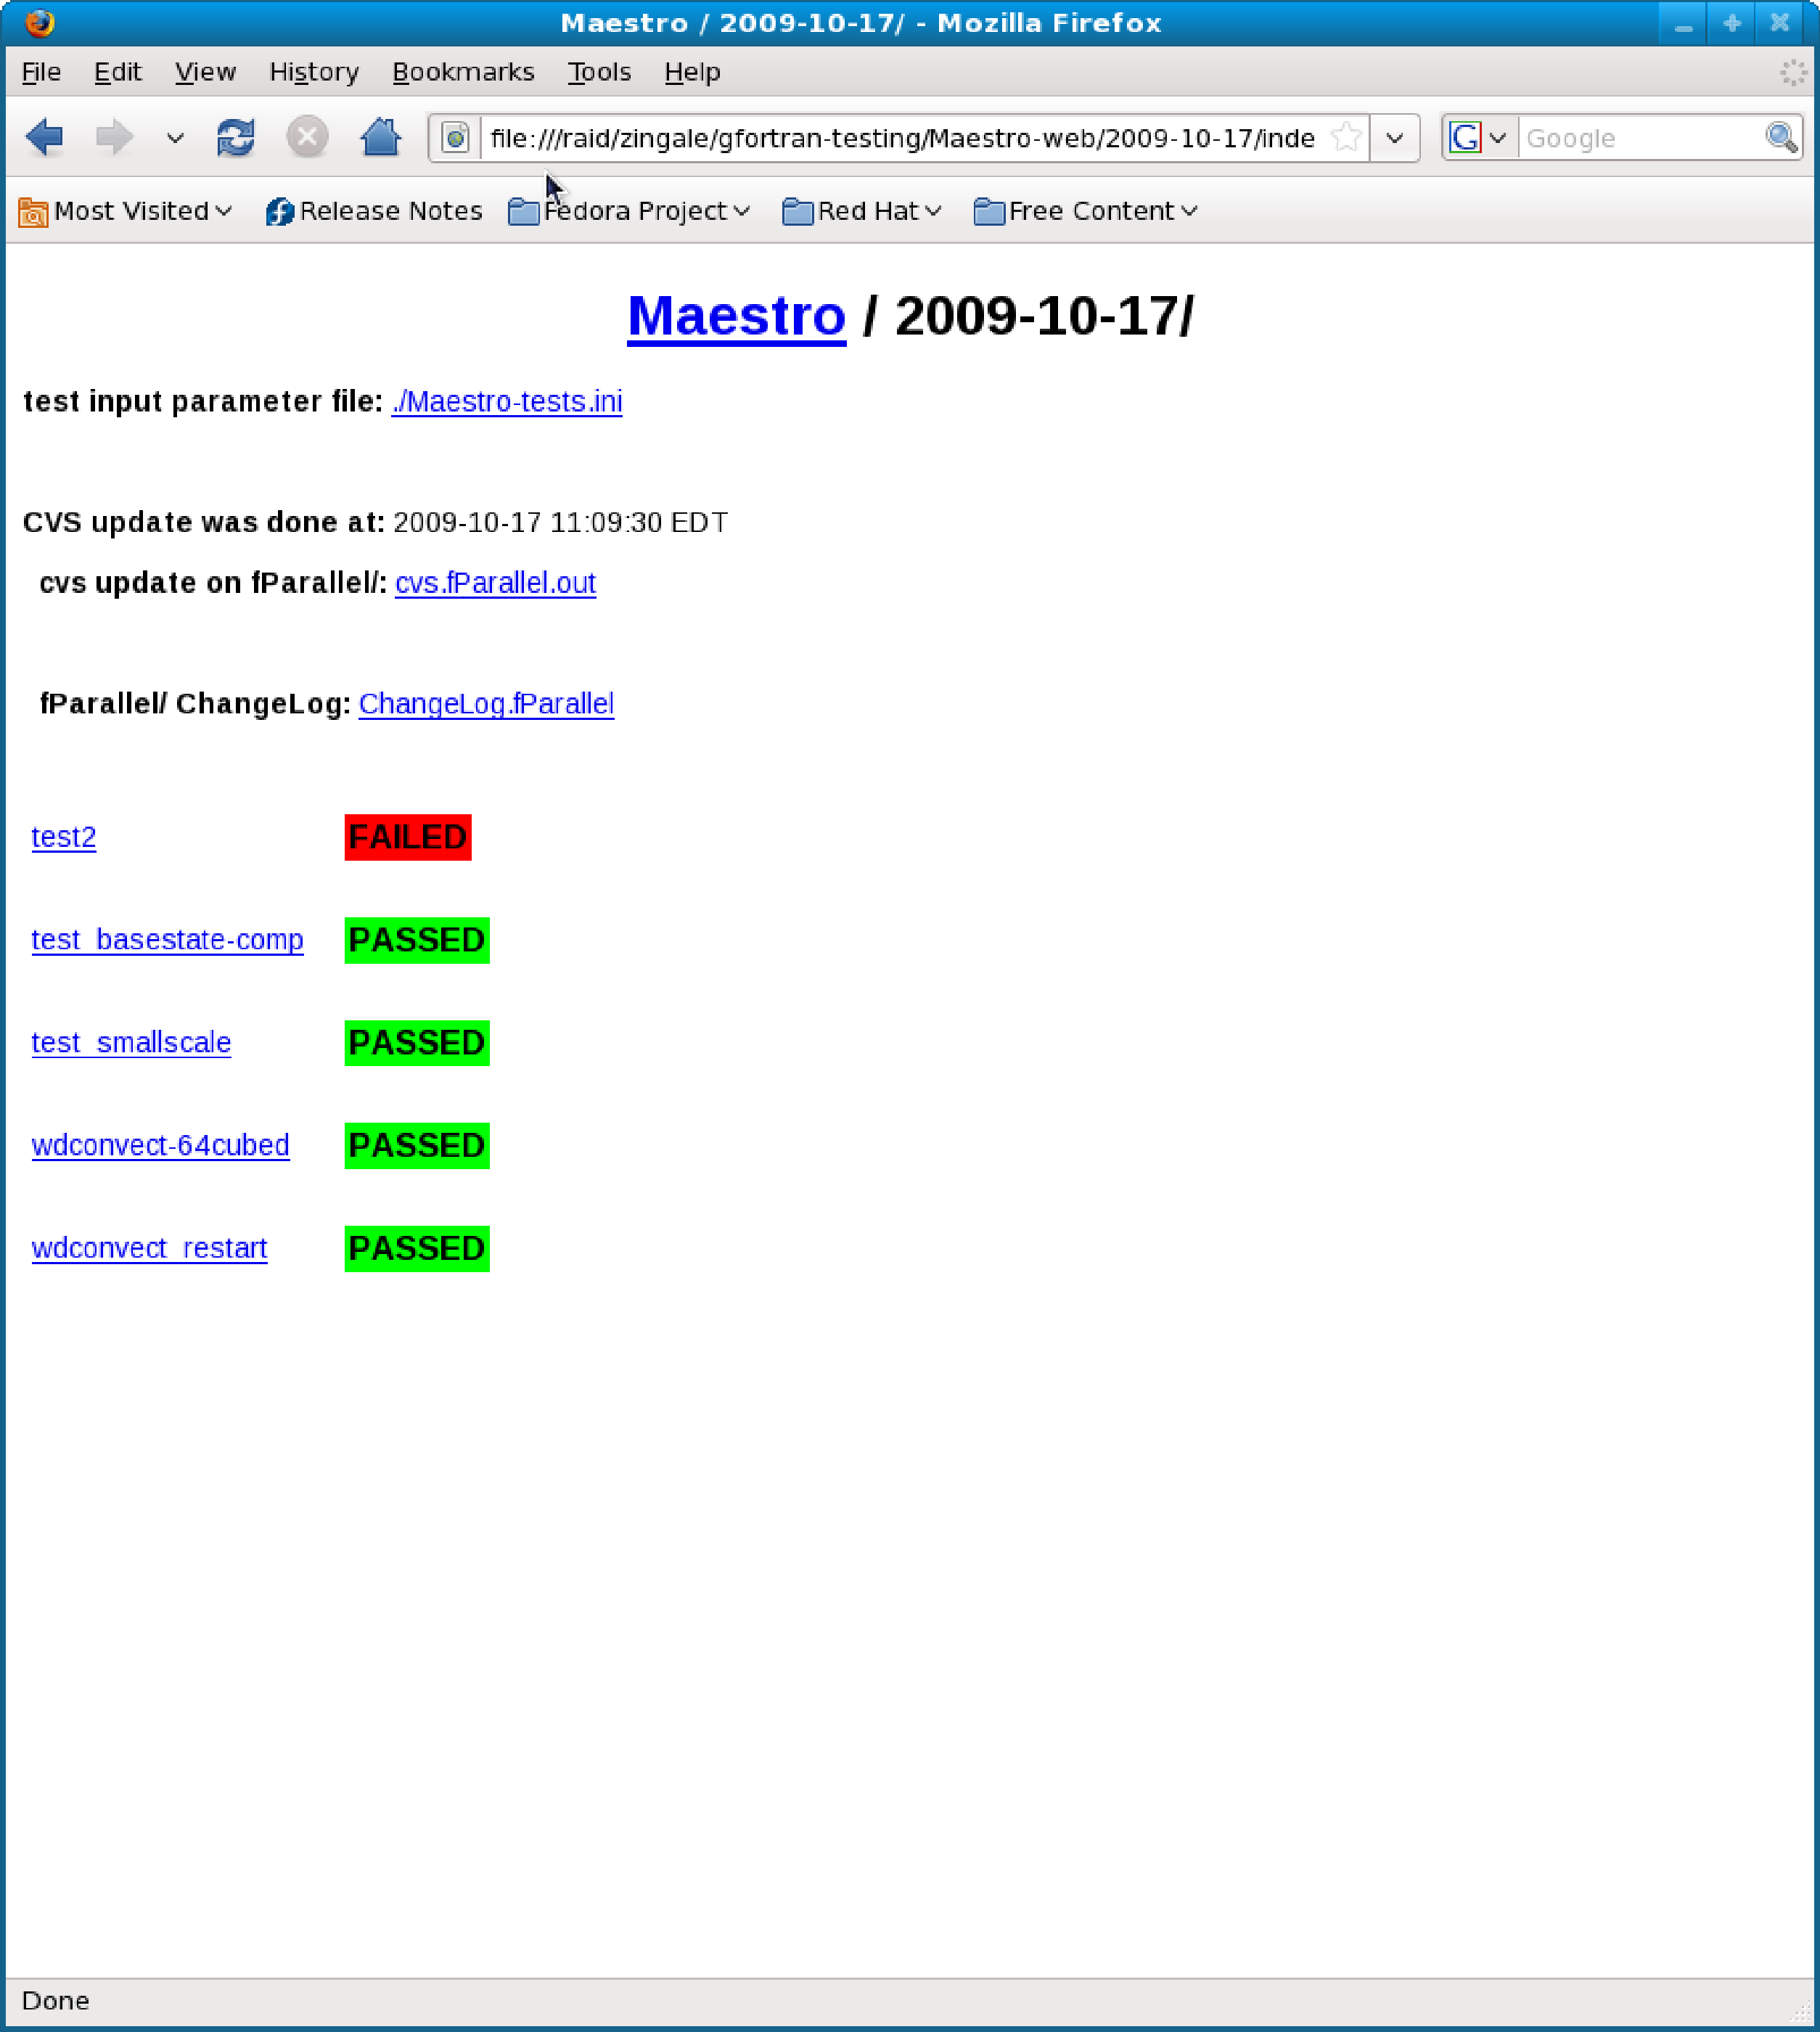
\includegraphics[width=5.0in]{CastroVerification/test_suite_day}
\caption{\label{fig:test_suite_date} The test suite output for a
  single day's run.  Each row indicates a separate test, showing
  whether they passed or failed.  Clicking on the test name will give
  more information about that particular test on that day. Note: this
  page is from the {\tt Maestro} code, but a {\tt Castro} test suite
  run will produce similar output.}
\end{figure}

Upon completion of all the runs, a web page for this invocation of the
test suite will be generated (see figure~\ref{fig:test_suite_date}),
as well as pages showing the details for each of the problems run.
Test failures indicate that the current output does not match the stored
benchmarks.


\subsection{Updating Benchmarks}

A test failure means that the current version of the code gives a
different answer than the stored benchmark.  A test can fail either
because a bug was introduced into the code or a bug was fixed or new
feature introduced.

If a bug was introduced into the code recently, then by examing the
test history you can determine the time period in which the bug was
introduced.  The {\tt ChangeLog.Parallel} and {\tt
  ChangeLog.fParallel} files linked to on each test date's webpage
will list all the changes committed to CVS up to that point, which is
useful for tracking down the bug.  Once the bug is fixed, rerunning
the suite should generate a `pass'.

If a bug was fixed or a new feature was introduced, and you are
confident that the latest output is correct, then you can tell the
test suite to update the benchmarks.  If you want to do this for all
the test problems, you would do:\\
$~~~~~${\tt ./test.py --make\_benchmarks "X bug fixed" ./Castro\_tests.ini} \\
where the string after ``{\tt --make\_benchmarks}'' is a note that is listed
on the regression suite web page describing the reason for the benchmark
update.  Subsequent runs of the test suite will use the new benchmarks.
If you only want to update the benchmarks of a single test, then you
can use the ``{\tt --single\_test test}'' flag on the commandline, where
{\tt test} is the name of the test to update.




%------------------------------------------------------------------------------
\backmatter

\renewcommand\bibname{References}
\addcontentsline{toc}{chapter}{References}
\bibliographystyle{plain}
\bibliography{refs,Verification/verification,Gravity/gr}

\cleardoublepage
\phantomsection
\addcontentsline{toc}{chapter}{Index}
\printindex

\end{document}
